\documentclass[a4paper,12pt]{report}

% Language setting
\usepackage[utf8]{inputenc}
% T1 podrazumevano (latinica), T2A za cirilicni naslov.
% Ako cirilicna podrska nije instalirana (paket texlive-lang-cyrillic),
% naslov privremeno pada na latinicu da bi se rad ipak kompajlirao.
\IfFileExists{t2aenc.def}{%
  \usepackage[T2A,T1]{fontenc}%
  \newcommand{\naslovcir}{{\fontencoding{T2A}\selectfont Криптографски акцелератор на FPGA платформи заснован на ECDH, SHA-3 и AES-GCM алгоритмима}}%
}{%
  \usepackage[T1]{fontenc}%
  \newcommand{\naslovcir}{Kriptografski akcelerator na FPGA platformi zasnovan na ECDH, SHA-3 i AES-GCM algoritmima}%
}
\usepackage[serbian]{babel}
% babel-serbian pravi znak " aktivnim (precica za prelom i navodnike). U radu se "
% koristi doslovno, npr. u \texttt{"KMAC"}, pa se precica iskljucuje.
% \AtBeginDocument je nuzan: babel precice ponovo ukljucuje pri izboru jezika.
\AtBeginDocument{\shorthandoff{"}}

% Set page size and margins
\usepackage[a4paper,top=2cm,bottom=2cm,left=3cm,right=3cm,marginparwidth=1.75cm]{geometry}

\setcounter{secnumdepth}{3}
\setcounter{tocdepth}{3}

% Useful packages
\usepackage{amsmath}
\DeclareMathOperator{\sgn}{sgn}
\DeclareMathOperator{\adj}{adj}
\usepackage{amsfonts}
\usepackage{amssymb}
\usepackage{graphicx}
\usepackage{caption}
\usepackage{subcaption}
\usepackage{tikz}
\usetikzlibrary{matrix, positioning, automata, arrows, calc, patterns, fit, shapes.geometric}
\usepackage[colorlinks=true, allcolors=blue]{hyperref}

\usepackage{float}
\usepackage{listings}
\PassOptionsToPackage{table}{xcolor}
\usepackage{pgfplots}
\pgfplotsset{compat=1.16}
\usepackage{mathtools}
\usepackage{enumerate}
\usepackage{enumitem}
\usepackage{array}
\usepackage{placeins}
\usepackage{multirow}
\usepackage{colortbl}
\usepackage{makecell}
\usepackage{arydshln} % Za napredne linije i kontrolu debljine
\usepackage{textcomp}
\usepackage{bm}
\usepackage{etoolbox} % velicina tabela, kontrola
\usepackage{booktabs} % kontrola debljina linija u tabelama

\usepackage{amsthm}
% Definisanje okruzenja 'example'
\newtheorem{example}{Primer}[chapter]

\newcolumntype{B}{>{\bfseries}l} % auto bold
\newcommand{\rsz}[3][1cm]{%resize za tabele
  \makebox[#1][c]{\resizebox{#2\width}{!}{#3}}%
}

\setlength{\arrayrulewidth}{0.5mm} % Adjust table line thickness
\setlength{\tabcolsep}{15pt} % Adjust column separation
\renewcommand{\arraystretch}{2} % Adjust row height

% Kvadratne celije za seme matrica (stanje Keccak-a, matrica stanja AES-a).
% Sirina celije = 1cm (\rsz) + 2*tabcolsep, visina = arraystretch * baselineskip(\Large);
% vrednosti 10pt i 2.35 izjednacavaju to dvoje, pa celije ispadaju kvadratne.
\newcommand{\kvsetup}{\Large\setlength{\tabcolsep}{10pt}\renewcommand{\arraystretch}{2.35}}
\newcommand{\kv}[1]{\rsz{1.4}{#1}}

% Prelom reci koristi srpske uzorke (hyph-sr-latn), iz paketa texlive-lang-cyrillic;
% TeX Live srpski svrstava medju cirilicne jezike bez obzira na pismo. Rucna lista
% izuzetaka koja je ranije stajala ovde vise nije potrebna.
%
% Nazivi (Slika, Tabela, Poglavlje...) se prepisuju posle \begin{document}, jer bi
% ih babel inace postavio na svoje.

\sloppy

\definecolor{codegreen}{rgb}{0,0.6,0}
\definecolor{codegray}{rgb}{0.5,0.5,0.5}
\definecolor{codepurple}{rgb}{0.58,0,0.82}
\definecolor{backcolour}{rgb}{0.95,0.95,0.92}

\lstdefinestyle{mystyle}{
    backgroundcolor=\color{backcolour},
    commentstyle=\color{codegreen},
    keywordstyle=\color{magenta},
    numberstyle=\tiny\color{codegray},
    stringstyle=\color{codepurple},
    basicstyle=\ttfamily\footnotesize,
    breakatwhitespace=false,
    breaklines=true,
    captionpos=b,
    keepspaces=true,
    numbers=left,
    numbersep=5pt,
    showspaces=false,
    showstringspaces=false,
    showtabs=false,
    tabsize=2
}
\lstset{style=mystyle}

% Imenovani TikZ stilovi za seme (boje konzistentne kroz ceo rad, kao u diplomskom):
% blokdata = podaci (zeleno), blokkripto = kriptografska operacija (zuto),
% blokrezultat = izlaz/kriptogram (ljubicasto), blokghash = autentifikacija (cijan)
\tikzstyle{blokdata} = [rectangle, rounded corners, minimum width=2.2cm, minimum height=0.9cm, text centered, draw=black, fill=green!30]
\tikzstyle{blokkripto} = [rectangle, rounded corners, minimum width=2.2cm, minimum height=0.9cm, text centered, draw=black, fill=yellow!30]
\tikzstyle{blokrezultat} = [rectangle, rounded corners, minimum width=2.2cm, minimum height=0.9cm, text centered, draw=black, fill=purple!30]
\tikzstyle{blokghash} = [rectangle, rounded corners, minimum width=2.2cm, minimum height=0.9cm, text centered, draw=black, fill=cyan!30]
\tikzstyle{strelica} = [thick,->,>=stealth]
% Stil za masine stanja: sivi krugovi i sive strelice, crni natpisi
\tikzstyle{fsm} = [->, >=stealth, auto,
    every state/.style={circle, draw=black!55, line width=1.1pt, fill=gray!12, minimum size=1.9cm, font=\small\ttfamily},
    every edge/.style={draw=black!55, line width=1.1pt, ->, >=stealth},
    every initial by arrow/.style={draw=black!55, line width=1.1pt, ->, >=stealth},
    initial text={\itshape reset}]

\title{\Huge\vspace{10mm}{\bf{\naslovcir}}}
\author{\textsl{\vspace{10mm}Marko Gavrilović}}
\date{\vspace{120mm}2026.}

\begin{document}

\renewcommand*\contentsname{Sadržaj}
\renewcommand{\figurename}{Slika}
\renewcommand{\lstlistingname}{Tekst}
\renewcommand{\tablename}{Tabela}
\renewcommand{\chaptername}{Poglavlje}
\renewcommand{\listfigurename}{Lista slika}
\renewcommand{\listtablename}{Lista tabela}
\renewcommand\bibname{Reference}

\newcommand*{\defeq}{\stackrel{\text{def}}{=}}
\newcommand*{\textarrowright}[1]{\stackrel{\text{#1}}{\longrightarrow}}
\newcommand*{\arrowtext}[1]{\stackrel{\rightarrow}{\text{#1}}}

\newcommand*{\vertbar}{\rule[-1ex]{0.5pt}{2.5ex}}
\newcommand*{\horzbar}{\rule[.5ex]{2.5ex}{0.5pt}}
\newcommand{\iu}{{i\mkern1mu}}

\begin{sffamily}
\thispagestyle{empty}
{\fontencoding{T2A}\selectfont
\begin{center}%
 	{\large{\scshape{Универзитет у Београду}\\[.5ex]\textsc{Електротехнички факултет}} \par}
 	 \vskip 12ex
    {\large {
\includegraphics[scale = 0.5]{etf-pecat.png}}\par}%
      \vskip 12ex
    {\LARGE \naslovcir\par}%
    \vskip 2ex%
    {\large
	Мастер рад \par
    }
  \end{center}\par
    \vfill \vfill
  Студент: \hspace*{\fill} Ментор: \par
  Марко Гавриловић, 2024/3101 \hspace*{\fill} др Владимир Петровић, доцент \par

  \vfill
\begin{center}
{\large Београд, 2026.}
\end{center}
}
\end{sffamily}

\newpage
\tableofcontents
\newpage

\listoffigures
\addcontentsline{toc}{chapter}{Lista slika}

\listoftables

\chapter{Uvod}
\label{ch:uvod}

Savremeni svet počiva na razmeni digitalnih informacija. Količina podataka koja se svakodnevno prenosi kroz računarske mreže neprestano raste, a sa njom i potreba da ti podaci budu zaštićeni, kako od neovlašćenog čitanja, tako i od neprimetne izmene. Kriptografija, nekada disciplina rezervisana za vojne i diplomatske potrebe, danas je ugrađena u gotovo svaki aspekt digitalnog života, od onlajn bankarstva i elektronske trgovine, preko virtuelnih privatnih mreža, do komunikacije uređaja u industrijskim postrojenjima i automobilima.
\smallbreak
Zaštita komunikacije u praksi nikada ne počiva na jednom kriptografskom algoritmu. Bezbedan komunikacioni kanal zahteva rešavanje više nezavisnih problema. Dve strane najpre moraju da uspostave zajednički tajni ključ preko nezaštićenog medijuma, zatim da iz tog zajedničkog materijala izvedu ključeve sesije, i konačno da svaku poruku šifruju tako da primalac može da proveri i njenu poverljivost i njen integritet. Moderni protokoli, poput TLS-a (engl. \textit{Transport Layer Security}) ili IPsec-a, zbog toga kombinuju više algoritama različitih klasa u jedinstven hibridni kriptosistem: asimetrične algoritme za razmenu ključeva, heš funkcije za izvođenje ključeva i proveru integriteta, i simetrične šifre za zaštitu samih podataka.
\smallbreak
Sa porastom brzina mrežnih interfejsa, softverska realizacija ovih algoritama na procesorima opšte namene postaje usko grlo. Kriptografske operacije su računski intenzivne, a njihovo izvršavanje na procesoru troši resurse koji bi mogli biti iskorišćeni za samu aplikaciju. Prirodno rešenje je izmeštanje kriptografskih operacija u namenski hardver, takozvani kriptografski akcelerator. FPGA (engl. \textit{Field Programmable Gate Array}) platforme su za ovu namenu posebno pogodne, jer nude paralelizam i propusnost blisku namenskim integrisanim kolima, uz zadržavanje fleksibilnosti rekonfiguracije, što je značajno u oblasti u kojoj se standardi i preporuke vremenom menjaju. Kao ciljna platforma u ovom radu izabran je razvojni sistem Kria KR260, sa čipom Zynq UltraScale+ MPSoC. Taj čip na istom silicijumu objedinjuje programabilnu logiku i procesorski sistem, pa akcelerator može da radi samostalno, ali i pod upravom softvera koji se izvršava na istom čipu. Ta mogućnost iskorišćena je za ispitivanje jednog od realizovanih jezgara na ploči, preko namenskog upravljačkog programa.
\smallbreak
Cilj ovog rada je projektovanje kriptografskog akceleratora na FPGA platformi koji objedinjuje tri algoritma savremene kriptografije, po jedan iz svake ključne klase:
\begin{itemize}[itemsep=2pt]
    \item ECDH (engl. \textit{Elliptic Curve Diffie--Hellman}) -- protokol za uspostavljanje zajedničkog tajnog ključa zasnovan na eliptičkim krivama, realizovan nad binarnim poljem korišćenjem krive B-571;
    \item SHA-3 (engl. \textit{Secure Hash Algorithm 3}) -- standardizovana kriptografska heš funkcija zasnovana na Keccak algoritmu, korišćena kroz KMAC konstrukciju za izvođenje ključeva i proveru integriteta;
    \item AES-GCM (engl. \textit{Advanced Encryption Standard -- Galois/Counter Mode}) -- autentifikovana simetrična šifra koja u jednom prolazu obezbeđuje i poverljivost i integritet podataka.
\end{itemize}
\smallbreak
Ova tri algoritma zajedno čine funkcionalnu celinu u kojoj ECDH obezbeđuje zajedničku tajnu, SHA-3 iz nje izvodi ključeve sesije, a AES-GCM tim ključevima štiti korisnički saobraćaj. Za potpun bezbedan sistem neophodna je još i autentifikacija učesnika u razmeni ključeva, koja se tipično ostvaruje algoritmom digitalnog potpisa kao što je ECDSA (engl. \textit{Elliptic Curve Digital Signature Algorithm}). Njegova realizacija prevazilazi obim ovog rada, ali je njegova uloga u sistemu razmotrena na odgovarajućim mestima.
\smallbreak
Sve hardverske arhitekture opisane u radu realizovane su u jeziku za opis hardvera VHDL, korišćenjem alata AMD Vivado. Provera je izvedena na više nivoa, simulacijom nad standardizovanim test vektorima, namenskim testovima graničnih slučajeva i merenjem na samoj ploči. SHA-3 akcelerator pušten je pod operativnim sistemom PetaLinux, preko upravljačkog programa napisanog za tu namenu, a AES-GCM akcelerator proveren je umetnut u postojeći mrežni sistem. Pored hardverskih realizacija, razvijeni su i softverski referentni modeli, koji služe za proveru ispravnosti i kao osnova za poređenje performansi.
\smallbreak
Rad je organizovan na sledeći način. U drugom poglavlju dat je pregled osnovnih pojmova kriptografije, od sigurnosnih zahteva i klasa algoritama do načina na koji se oni kombinuju u hibridni kriptosistem kakav je realizovan u ovom radu.
\smallbreak
Treće poglavlje teorijski obrađuje tri korišćena algoritma, od matematičkih osnova eliptičkih krivih i ECDH protokola, preko sponge konstrukcije i Keccak permutacije na kojima počiva SHA-3, do AES algoritma u GCM režimu rada sa pripadajućom GHASH funkcijom.
\smallbreak
U četvrtom poglavlju opisane su hardverske arhitekture akceleratora za svaki od algoritama i njihova integracija u sistem.
\smallbreak
Peto poglavlje prikazuje metodologiju verifikacije i postignute rezultate, zauzeće resursa, radne učestanosti, latenciju skalarnog množenja i propusnost, uz poređenje SHA-3 jezgra sa softverskim realizacijama.
\smallbreak
Šesto poglavlje razmatra moguća unapređenja, od zaokruživanja sistema na ploči, preko pomeranja granice propusnosti puta podataka, do razvoja upravljačke ravni i postkvantne zamene razmene ključa, a sedmo donosi zaključak.

\chapter{Kriptografske osnove}
\label{ch:osnove}

Ovo poglavlje uspostavlja pojmovni okvir na kome počiva ostatak rada: model komunikacije i osnovnu terminologiju, sigurnosne zahteve koje savremeni komunikacioni sistem mora da ispuni, tri klase kriptografskih algoritama i način na koji se one povezuju u hibridni kriptosistem kakav je realizovan u ovom radu. Sistematičan i detaljniji uvod u kriptografiju dat je u \cite{paar_pelzl, katz_lindell}.

\section{Osnovni pojmovi i model komunikacije}
\label{sec:osnovni_pojmovi}

Kriptografija proučava tehnike zaštite informacija u prisustvu protivnika. Standardni model podrazumeva dve strane koje komuniciraju preko nezaštićenog kanala i protivnika koji taj kanal može da prisluškuje, a u opštem slučaju i da aktivno menja, briše ili ubacuje poruke. Pošiljalac se tradicionalno zove Alisa, primalac Bob, a protivnik Oskar. U literaturi se sreću i druga imena, najčešće Eva za pasivnog prisluškivača i Malori za aktivnog napadača. U ovom radu dosledno se koristi Oskar, prema konvenciji iz \cite{paar_pelzl}, i to za obe vrste protivnika.
\smallbreak
Postupak transformacije izvorne poruke, otvorenog teksta (engl. \textit{plaintext}), u nečitljiv oblik, šifrat (engl. \textit{ciphertext}), naziva se šifrovanje (engl. \textit{encryption}), a obrnuti postupak dešifrovanje (engl. \textit{decryption}). Obe transformacije parametrizovane su ključem. Prema Kerckhoffsovom principu (engl. \textit{Kerckhoffs's principle}), formulisanom još 1883. godine \cite{kerckhoffs1883}, sigurnost sistema ne sme počivati na tajnosti samog algoritma, već isključivo na tajnosti ključa. Algoritam se smatra javno poznatim, a jedino što Oskar ne poznaje jeste ključ. Ovaj princip je danas univerzalno prihvaćen \cite{paar_pelzl}, pa su svi algoritmi korišćeni u ovom radu javni, međunarodno standardizovani i detaljno proučeni u stručnoj zajednici.

\section{Sigurnosni zahtevi}
\label{sec:sigurnosni_zahtevi}

Bezbedan komunikacioni sistem mora da obezbedi više međusobno nezavisnih svojstava. Za ovaj rad ključna su sledeća četiri.
\smallbreak
\textit{Poverljivost} (engl. \textit{confidentiality}) garantuje da sadržaj poruke ostaje nedostupan svakome ko ne poseduje odgovarajući ključ. Ovo je istorijski najstariji i najintuitivniji zahtev kriptografije. Oskar, koji prisluškuje kanal, ne može iz šifrata da rekonstruiše otvoreni tekst, niti da o njemu sazna bilo koju delimičnu informaciju.
\smallbreak
\textit{Integritet} (engl. \textit{integrity}) garantuje da poruka nije izmenjena na putu od pošiljaoca do primaoca. Važno je uočiti da poverljivost sama po sebi ne obezbeđuje integritet. Kod mnogih šifara protivnik može ciljano da izmeni šifrat tako da izazove predvidljivu promenu dešifrovanog teksta, ne znajući pritom ključ. Zbog toga se integritet mora obezbediti posebnim mehanizmima, kao što su kodovi za autentifikaciju poruka (engl. \textit{Message Authentication Code}, MAC). Bitno je da takav kod koristi ključ. Običan sažetak štiti samo od slučajnih izmena, jer ga protivnik može preračunati zajedno sa izmenjenom porukom, dok oznaku izračunatu sa tajnim ključem može proizvesti isključivo onaj ko taj ključ poseduje.
\smallbreak
\textit{Autentičnost} (engl. \textit{authenticity}) garantuje da poruka zaista potiče od strane koja tvrdi da ju je poslala. Korisno je razlikovati dva nivoa, poreklo pojedinačne poruke i identitet učesnika u vezi. \textit{Autentičnost porekla poruke} sledi neposredno iz mehanizma integriteta. Pošto ispravnu oznaku može izračunati samo posednik ključa, MAC istovremeno obezbeđuje i integritet i poreklo, pa se ta dva svojstva u praksi i ne razdvajaju. \textit{Autentičnost učesnika} je, međutim, pitanje ko se uopšte nalazi na drugom kraju veze, i ono se mora rešiti pre nego što zajednički ključ i postoji. Ako Alisa ne može da proveri da pregovara baš sa Bobom, Oskar može da se postavi između njih i sa svakim od njih uspostavi zaseban ključ, u napadu poznatom kao čovek u sredini (engl. \textit{man-in-the-middle}, MITM). Ovaj drugi nivo ostvaruje se digitalnim potpisima i infrastrukturom javnih ključeva.
\smallbreak
Dva nivoa se dopunjuju, a ne zamenjuju. Oznaka koju računa režim autentifikovanog šifrovanja (odeljak \ref{subsubsec:aead}) dokazuje samo da poruka potiče od one strane sa kojom je ključ uspostavljen. Ako sama uspostava ključa nije autentifikovana, ta strana može biti i Oskar, pa otuda i redosled u protokolu. Potpis štiti razmenu ključeva, a oznaka štiti saobraćaj kada ključ već postoji.
\smallbreak
\textit{Svežina poruka} je četvrti zahtev. Čak i kada su poverljivost, integritet i autentičnost obezbeđeni, Oskar može da snimi ispravnu šifrovanu poruku i da je kasnije ponovo pošalje, u napadu ponavljanjem (engl. \textit{replay attack}). Odbrana traži da svaka poruka nosi element koji se ne ponavlja, a takva vrednost se naziva nonce (engl. \textit{number used once}): redni broj, vremenska oznaka ili nasumična vrednost dovoljne dužine.
\smallbreak
Nonce vrednost se u ovom radu javlja u dve uloge, i jedna ne zamenjuje drugu. Kao mehanizam svežine, treba da omogući primaocu da odbaci poruku koju je već video. Unutar GCM režima, gde nonce ulazi kroz parametar koji standard zove inicijalizacioni vektor (engl. \textit{initialization vector}, $IV$), zahtev da $IV$ bude jedinstven obavezuje samo pošiljaoca, i to zato da isti pseudoslučajni niz ne upotrebi dvaput. Primalac pri tome ne pamti koje je vrednosti $IV$ ranije primio, pa snimljen paket sa svojim izvornim $IV$ i ispravnom oznakom prolazi proveru i drugi put. Zaštita od ponavljanja je zato zaseban mehanizam na nivou protokola, tipično brojač sekvence i prozor prihvatanja kod primaoca, i nije deo GCM režima.
\smallbreak
Tabela \ref{tab:zahtevi} povezuje ova četiri zahteva sa mehanizmima kojima se ostvaruju i sa njihovom realizacijom u sistemu opisanom u ovom radu.

\begin{table}[H]
\caption{Sigurnosni zahtevi, mehanizmi i njihova realizacija u ovom radu}
\centering
\setlength{\tabcolsep}{5pt}
\renewcommand{\arraystretch}{1.4}
\resizebox{\textwidth}{!}{
\begin{tabular}{|c|c|c|}
\hline
\rowcolor{gray!30}
Zahtev & Mehanizam & Realizacija u ovom radu \\
\hline
poverljivost & simetrično šifrovanje & AES u CTR režimu (deo GCM-a) \\
\hline
\makecell{integritet i\\autentičnost poruke} & \makecell{kod za autentifikaciju\\poruka (MAC)} & GHASH i oznaka u GCM režimu \\
\hline
autentičnost učesnika & \makecell{digitalni potpis\\i sertifikati} & \makecell{ECDSA, predviđena\\nadogradnja} \\
\hline
svežina poruka & \makecell{brojač sekvence i\\prozor prihvatanja} & van obima rada \\
\hline
\end{tabular}
}
\label{tab:zahtevi}
\end{table}

\section{Klase kriptografskih algoritama}
\label{sec:klase_algoritama}

Savremeni kriptografski algoritmi dele se u tri osnovne klase, koje se međusobno razlikuju po načinu upotrebe ključeva i po problemima koje rešavaju.

\subsection{Algoritmi sa simetričnim ključem}
\label{subsec:simetricni}

Kod simetričnih algoritama obe strane koriste isti tajni ključ i za šifrovanje i za dešifrovanje. Glavne predstavnike čine blok šifre (engl. \textit{block cipher}), koje podatke obrađuju u blokovima fiksne dužine, i protočne šifre (engl. \textit{stream cipher}), koje generišu pseudoslučajni niz kojim se otvoreni tekst kombinuje bit po bit. Najznačajniji savremeni predstavnik blok šifara je AES, usvojen 2001. godine kao američki federalni standard za obradu informacija (engl. \textit{Federal Information Processing Standard}, FIPS) pod oznakom FIPS 197 \cite{fips197}.
\smallbreak
AES nije jedini simetrični algoritam u upotrebi. Trostruka primena starijeg standarda DES (engl. \textit{Data Encryption Standard}), poznata kao 3DES, dugo je bila standard u bankarskim sistemima, ali ju je američki Nacionalni institut za standarde i tehnologiju (engl. \textit{National Institute of Standards and Technology}, NIST) povukao iz upotrebe zbog kratkog bloka od 64 bita i niske brzine \cite{sp800131a}. Protočna šifra ChaCha20, u sprezi sa autentifikatorom Poly1305, standardizovana je za internet protokole \cite{rfc8439} i koristi se u TLS-u 1.3. Njena je posebnost to što je izrazito brza u softveru, na procesorima bez namenskih instrukcija za AES, što je upravo suprotan slučaj od onog koji ovaj rad razmatra. Za uređaje sa strogo ograničenim resursima NIST je 2025. godine standardizovao porodicu ASCON \cite{ascon}. AES je ovde izabran jer je i dalje osnovni standard, jer ga podržava GCM režim rada, i jer je njegova struktura izrazito pogodna za hardversku realizaciju.
\smallbreak
Simetrični algoritmi su računski efikasni i pogodni za hardversku realizaciju, pa se praktično sav korisnički saobraćaj u savremenim protokolima štiti upravo njima. Njihova suštinska slabost je problem distribucije ključa. Pre početka komunikacije obe strane moraju posedovati isti tajni ključ, a njega je nemoguće bezbedno preneti preko istog nezaštićenog kanala koji tek treba zaštititi.

\subsubsection{Režimi rada blok šifara}
\label{subsubsec:rezimi_rada}

Blok šifra sama po sebi definiše transformaciju samo nad jednim blokom fiksne dužine, kod AES-a 128 bitova. Način na koji se šifra primenjuje na poruke proizvoljne dužine definiše režim rada (engl. \textit{mode of operation}) \cite{sp80038a}. Režimi se razlikuju i po sigurnosnim svojstvima i po pogodnosti za hardversku realizaciju. Poređenje tri karakteristična režima dato je u odeljku \ref{subsec:rezimi_rada_detaljno}. Za klasifikaciju je ključno da nijedan od njih sam po sebi ne obezbeđuje integritet poruke.

\subsubsection{Autentifikovano šifrovanje}
\label{subsubsec:aead}

Pošto poverljivost i integritet zahtevaju odvojene mehanizme, a njihovo nezavisno kombinovanje se u praksi pokazalo sklono suptilnim greškama, razvijeni su režimi autentifikovanog šifrovanja sa pridruženim podacima (engl. \textit{Authenticated Encryption with Associated Data}, AEAD). AEAD režim u jednom prolazu šifruje poruku i računa autentifikacionu oznaku (engl. \textit{authentication tag}) nad šifratom i pridruženim podacima koji se prenose nešifrovani, na primer nad zaglavljima mrežnih paketa. Primalac odbacuje svaku poruku čija oznaka nije ispravna, pre nego što dešifrovani sadržaj uopšte postane dostupan aplikaciji. Najrasprostranjeniji AEAD režim danas je GCM (engl. \textit{Galois/Counter Mode}) \cite{sp80038d}, koji kombinuje CTR režim šifrovanja sa autentifikacijom zasnovanom na množenju u Galoisovom polju. Njegova konstrukcija detaljno je opisana u odeljku \ref{sec:aes_gcm}.
\smallbreak
GCM nije jedini AEAD režim. Postoje i konstrukcije koje autentifikaciju ostvaruju samom blok šifrom, bez zasebne aritmetičke jedinice. Režim OCB \cite{rfc7253} postiže autentifikovano šifrovanje u jednom prolazu koristeći isključivo pozive blok šifre, pa u hardveru ne zahteva množač u Galoisovom polju. Njegovo šire usvajanje dugo je kočilo patentno opterećenje, koje je uklonjeno tek 2021. godine. Režim CCM \cite{sp80038c}, korišćen u standardu WPA2, takođe se oslanja samo na blok šifru, ali zahteva dva prolaza kroz podatke, što ga čini nepogodnim za obradu u liniji. Detaljnija razmatranja ovih režima mogu se naći u navedenim standardima, uz napomenu da je raniji OCB2 kriptoanalitički oboren \cite{inoue_ocb2}, dok OCB3 i dalje važi za siguran. U ovom radu izabran je GCM jer je standard u protokolima TLS, IPsec i MACsec, radi u jednom prolazu i dopušta paralelnu obradu blokova. Cena tog izbora je namensko GHASH jezgro, čija je realizacija razmotrena u poglavlju \ref{ch:hardver}.

\subsection{Algoritmi sa asimetričnim ključem}
\label{subsec:asimetricni}

Asimetrična kriptografija, ili kriptografija javnog ključa, koju su konceptualno uveli Diffie i Hellman 1976. godine \cite{diffie_hellman}, rešava problem distribucije ključa. Svaki učesnik poseduje par matematički povezanih ključeva: javni, koji se slobodno objavljuje, i privatni, koji se čuva u tajnosti. Sigurnost počiva na postojanju jednosmernih funkcija sa zamkom, operacija koje je lako izračunati u jednom smeru, a praktično nemoguće invertovati bez poznavanja privatnog ključa.
\smallbreak
Klasični asimetrični sistemi, poput RSA algoritma, zasnivaju se na teškoći faktorizacije velikih brojeva. \textit{Kriptografija eliptičkih krivih} (engl. \textit{Elliptic Curve Cryptography}, ECC), koju su nezavisno predložili Koblitz i Miller sredinom 1980-ih \cite{koblitz, miller}, postiže ekvivalentnu sigurnost sa znatno kraćim ključevima. Sigurnosnom nivou RSA ključa od 3072 bita odgovara eliptička kriva reda veličine 256 bitova. Kraći ključevi znače manje memorije, brže operacije i manju potrošnju, što ECC čini posebno pogodnom za hardversku realizaciju.
\smallbreak
Asimetrični algoritmi su za nekoliko redova veličine sporiji od simetričnih, pa se u praksi ne koriste za šifrovanje samih podataka, već za dva specifična zadatka: razmenu ključeva (ECDH protokol, odeljak \ref{sec:ecdh}) i digitalno potpisivanje (na primer ECDSA algoritam), kojim se obezbeđuje autentičnost.

\subsection{Kriptografske heš funkcije}
\label{subsec:hash}

Kriptografska heš funkcija preslikava poruku proizvoljne dužine u sažetak (engl. \textit{digest}) fiksne dužine. Za razliku od šifara, heš funkcija ne koristi ključ, njena transformacija je javna i deterministička, i nije invertibilna. Iz sažetka se poruka ne rekonstruiše, jer se pri preslikavanju informacija nepovratno sažima.
\smallbreak
Da bi bila kriptografski upotrebljiva, heš funkcija mora ispunjavati tri svojstva:
\begin{itemize}[itemsep=2pt]
    \item \textit{otpornost na pronalaženje originala} (engl. \textit{preimage resistance}, u matematičkoj literaturi i praslika) -- za dati sažetak $h$ praktično je nemoguće naći poruku $m$ takvu da je $H(m)=h$;
    \item \textit{otpornost na pronalaženje drugog originala} (engl. \textit{second preimage resistance}) -- za datu poruku $m_1$ praktično je nemoguće naći drugu poruku $m_2 \neq m_1$ sa istim sažetkom;
    \item \textit{otpornost na kolizije} (engl. \textit{collision resistance}) -- praktično je nemoguće naći bilo koji par različitih poruka sa istim sažetkom.
\end{itemize}
\smallbreak
Poslednje svojstvo je najstrože, i ono određuje potrebnu dužinu sažetka. Zbog takozvanog rođendanskog paradoksa \cite{paar_pelzl}, koliziju u funkciji sa sažetkom od $n$ bitova moguće je naći nasumičnim probanjem posle približno
\begin{equation}
    2^{n/2}
    \label{eq:rodjendanska_granica}
\end{equation}
pokušaja, a ne $2^{n}$, koliko bi se naivno očekivalo. Sažetak stoga mora biti dvostruko duži od željenog nivoa sigurnosti. Funkcija SHA3-256 pruža 128 bitova otpornosti na kolizije, a SHA3-512 njih 256. Ta srazmera objašnjava izbor varijanti u ovom radu i biće ponovo korišćena pri usklađivanju sigurnosnih nivoa sva tri algoritma.
\smallbreak
Heš funkcije su univerzalni gradivni blok savremenih protokola, pa se koriste za proveru integriteta, u konstrukcijama MAC kodova, kod digitalnih potpisa, gde se potpisuje sažetak poruke a ne poruka sama, i za izvođenje ključeva (engl. \textit{key derivation}), odnosno transformaciju zajedničke tajne dobijene razmenom ključeva u kriptografski upotrebljive ključeve sesije. Upravo je poslednja uloga ta u kojoj heš funkcija učestvuje u sistemu opisanom u ovom radu.
\smallbreak
Aktuelni standard je SHA-3, zasnovan na Keccak algoritmu \cite{fips202}. Za razliku od porodice SHA-2, koja počiva na Merkle--Damgardovoj konstrukciji, SHA-3 koristi konstrukciju sunđera, pa kompromitacija jedne familije ne ugrožava drugu. Usput nema ni svojstvo produženja poruke (engl. \textit{length extension}). Okolnosti pod kojima je standard nastao razmotrene su u odeljku \ref{sec:sha3}.
\smallbreak
Tabela \ref{tab:klase} sumira osnovne razlike između tri opisane klase.

\begin{table}[H]
\caption{Poređenje klasa kriptografskih algoritama}
\centering
\setlength{\tabcolsep}{5pt}
\renewcommand{\arraystretch}{1.4}
\resizebox{\textwidth}{!}{
\begin{tabular}{|c|c|c|c|c|}
\hline
\rowcolor{gray!30}
Klasa & Ključ & Brzina & Uloga & U ovom radu \\
\hline
simetrični & zajednički tajni & visoka & zaštita saobraćaja & AES-GCM \\
\hline
asimetrični & javni i privatni & niska & razmena ključeva i potpis & ECDH \\
\hline
heš funkcije & bez ključa & visoka & integritet i izvođenje ključeva & SHA-3 (KMAC) \\
\hline
\end{tabular}
}
\label{tab:klase}
\end{table}

\section{Hibridni kriptosistem}
\label{sec:hibridni_sistem}

Nijedna od opisanih klasa algoritama sama po sebi ne rešava sve sigurnosne zahteve iz odeljka \ref{sec:sigurnosni_zahtevi}. Simetrične šifre efikasno štite podatke, ali zahtevaju prethodno dogovoren ključ. Asimetrični algoritmi omogućavaju dogovor ključa preko javnog kanala, ali su prespori za zaštitu samog saobraćaja. Heš funkcije obezbeđuju integritet i izvođenje ključeva, ali same ne šifruju. Savremeni protokoli zato kombinuju sve tri klase u hibridni kriptosistem, u kome svaki algoritam obavlja zadatak za koji je najpogodniji.
\smallbreak
Akcelerator realizovan u ovom radu prati upravo ovu arhitekturu. Tok uspostavljanja i korišćenja bezbednog kanala odvija se u tri faze:
\begin{enumerate}[itemsep=2pt]
    \item \textit{Razmena ključeva (ECDH).} Alisa i Bob razmenjuju javne ključeve i, svako korišćenjem svog privatnog ključa, izračunavaju istu zajedničku tajnu. Oskar, koji prisluškuje kanal, vidi oba javna ključa, ali iz njih ne može izračunati zajedničku tajnu.
    \item \textit{Izvođenje ključeva (SHA-3).} Zajednička tajna dobijena ECDH razmenom nije uniformno raspodeljena i ne koristi se neposredno kao ključ. Umesto toga, propušta se kroz funkciju za izvođenje ključeva, u ovom radu KMAC konstrukciju zasnovanu na SHA-3 (odeljak \ref{subsec:kmac}), kojom se izvode ključ sesije i inicijalne vrednosti potrebne AEAD režimu.
    \item \textit{Zaštita saobraćaja (AES-GCM).} Izvedenim ključem sesije korisnički saobraćaj se šifruje u GCM režimu, koji svakom paketu pridružuje autentifikacionu oznaku, čime su poverljivost i integritet obezbeđeni u jednom prolazu.
\end{enumerate}
\smallbreak
Opisani tok prikazan je na slici \ref{fig:hibridni_tok}.

\begin{figure}[H]
\centering
\begin{tikzpicture}[node distance=1.0cm, font=\small]

% ----- naslovi strana -----
\node (alisa) at (-3.1, 0) {\textbf{Alisa}};
\node (bob)   at ( 3.1, 0) {\textbf{Bob}};
\node[draw=black, dashed, rounded corners, minimum width=1.9cm, minimum height=0.7cm,
      text centered, fill=gray!12] (oskar) at (0, 0) {Oskar};

% ----- faza 1: ECDH -----
\node[blokdata, below=0.7cm of alisa, minimum width=2.6cm] (privA) {privatni $d_A$};
\node[blokdata, below=0.7cm of bob,   minimum width=2.6cm] (privB) {privatni $d_B$};

\node[blokkripto, below=0.6cm of privA, minimum width=2.6cm] (mulA) {ECDH: $Q_A = d_A G$};
\node[blokkripto, below=0.6cm of privB, minimum width=2.6cm] (mulB) {ECDH: $Q_B = d_B G$};

% razmena javnih kljuceva preko nezasticenog kanala (dve paralelne vodoravne strelice)
\draw[strelica] ($(mulA.east)+(0,0.16)$) -- node[above, font=\scriptsize] {$Q_A$}
                ($(mulB.west)+(0,0.16)$);
\draw[strelica] ($(mulB.west)+(0,-0.16)$) -- node[below, font=\scriptsize] {$Q_B$}
                ($(mulA.east)+(0,-0.16)$);

\node[blokkripto, below=1.5cm of mulA, minimum width=2.6cm] (secA) {$Z = d_A Q_B$};
\node[blokkripto, below=1.5cm of mulB, minimum width=2.6cm] (secB) {$Z = d_B Q_A$};
\draw[strelica] (mulA) -- (secA);
\draw[strelica] (mulB) -- (secB);

% Oskar posmatra nezasticeni kanal
\coordinate (kanal) at ($(mulA.south)!0.5!(secA.north)$);
\draw[dashed, gray] (oskar.south) -- (kanal -| oskar);

% ----- faza 2: KDF -----
\node[blokdata, below=0.9cm of $(secA)!0.5!(secB)$, minimum width=4.4cm] (Z)
      {zajednička tajna $Z$};
% obe grane se spajaju u istu tacku, pa jedna strelica ulazi u Z
\coordinate (spoj) at ($(Z.north)+(0,0.35)$);
\draw[thick] (secA.south) |- (spoj);
\draw[thick] (secB.south) |- (spoj);
\draw[strelica] (spoj) -- (Z.north);

\node[blokghash, below=0.7cm of Z, minimum width=4.4cm] (kdf)
      {SHA-3 / KMAC: izvođenje ključeva};
\draw[strelica] (Z) -- (kdf);

\node[blokdata, below=0.7cm of kdf, minimum width=4.4cm] (K)
      {ključ sesije $K$, nonce};
\draw[strelica] (kdf) -- (K);

% ----- faza 3: AES-GCM -----
\node[blokkripto, below=0.7cm of K, minimum width=4.4cm] (gcm)
      {AES-GCM: šifrovanje i oznaka};
\draw[strelica] (K) -- (gcm);

\node[blokdata, left=1.1cm of gcm, minimum width=2.1cm] (pt) {otvoreni tekst};
\draw[strelica] (pt) -- (gcm);

\node[blokrezultat, below=0.7cm of gcm, minimum width=4.4cm] (ct)
      {šifrat $\mathrm{CT}$ i oznaka $\mathrm{ICV}$};
\draw[strelica] (gcm) -- (ct);

% ----- vodoravni razdelnici faza -----
\coordinate (sepA) at (0, 0.85);
\path (Z.south) -- (kdf.north) coordinate[midway] (sepB);
\path (K.south) -- (gcm.north) coordinate[midway] (sepC);
\coordinate (sepD) at ($(ct.south)+(0,-0.35)$);

\foreach \s in {sepA, sepB, sepC}{
    \draw[dashed, gray!65] ($(\s)+(-6.6,0)$) -- ($(\s)+(6.6,0)$);
}

% ----- naziv faze, sa desne strane i po sredini svog odeljka -----
\coordinate (desno) at (6.6, 0);
\path (sepA) -- (sepB) coordinate[midway] (sred1);
\path (sepB) -- (sepC) coordinate[midway] (sred2);
\path (sepC) -- (sepD) coordinate[midway] (sred3);

\node[anchor=east, align=right, text width=2.0cm, font=\footnotesize]
     at (desno |- sred1) {\textbf{1. faza}\\razmena\\ključeva};
\node[anchor=east, align=right, text width=2.0cm, font=\footnotesize]
     at (desno |- sred2) {\textbf{2. faza}\\izvođenje\\ključeva};
\node[anchor=east, align=right, text width=2.0cm, font=\footnotesize]
     at (desno |- sred3) {\textbf{3. faza}\\zaštita\\saobraćaja};

\end{tikzpicture}
\caption[Tok hibridnog kriptosistema]{Tok hibridnog kriptosistema realizovanog u ovom radu. Boje označavaju vrstu bloka: zelena su podaci, žuta
kriptografske operacije, cijan izvođenje ključeva, a ljubičasta zaštićeni izlaz.}
\label{fig:hibridni_tok}
\end{figure}

Sistem tako obezbeđuje poverljivost saobraćaja, njegov integritet i autentičnost porekla kroz oznaku koju računa GCM. Nonce vrednost pri tome čuva jedinstvenost pseudoslučajnog niza, dok zaštitu od ponovljenih poruka, po tabeli \ref{tab:zahtevi}, mora da obezbedi protokolski sloj iznad, tipično brojačem sekvence i prozorom prihvatanja. Preostaje zahtev autentičnosti učesnika. Bez potpisivanja javnih ključeva prva faza je ranjiva na napad čoveka u sredini, budući da Alisa nema način da utvrdi da javni ključ koji je primila zaista pripada Bobu, a ne Oskaru. U praksi se taj problem rešava digitalnim potpisom, tipično algoritmom ECDSA nad istom klasom eliptičkih krivih, u sprezi sa infrastrukturom sertifikata.
\smallbreak
Vredi naglasiti da dodavanje ECDSA nije puko proširenje već realizovanog hardvera. Sa ECDH protokolom ono deli samo skalarno množenje na krivoj, a pun obim nadogradnje, od aritmetike po modulu reda grupe do sabiranja dve nezavisne tačke pri proveri potpisa, razmatra odeljak \ref{sec:unap_sistem}.
\smallbreak
Preostaje da se vidi na kom nivou ceo lanac stoji. Sistem je jak koliko i njegova najslabija karika, pa parametri izabrani u poglavlju \ref{ch:algoritmi} nisu birani nezavisno, nego tako da svi budu na istom nivou. Pregled je dat u tabeli \ref{tab:nivoi_sigurnosti}.

\begin{table}[H]
\caption{Sigurnosni nivo pojedinih karika sistema. Nivo ECDH jezgra je polovina bitske dužine reda tačke (odeljak \ref{subsec:skalarno_mnozenje})}
\centering
\setlength{\tabcolsep}{5pt}
\renewcommand{\arraystretch}{1.4}
\resizebox{\textwidth}{!}{
\begin{tabular}{|c|c|c|}
\hline
\rowcolor{gray!30}
Uloga u sistemu & Algoritam i parametar & Sigurnosni nivo \\
\hline
razmena ključeva & ECDH nad krivom B-571 & $\approx 285$ bitova \\
\hline
izvođenje ključeva & KMAC256 & 256 bitova \\
\hline
šifrovanje & AES-256 & 256 bitova \\
\hline
autentifikacija poruke & \makecell{oznaka GCM\\od 128 bitova} & \makecell{128 bitova\\po pokušaju} \\
\hline
\end{tabular}
}
\label{tab:nivoi_sigurnosti}
\end{table}

Poslednji red odskače i traži objašnjenje, jer dužina oznake ne meri isto što i dužina ključa. Ključ štiti od čitanja saobraćaja, a oznaka od podmetanja izmenjene poruke. Napad na ključ izvodi se \textit{offline}, van veze, pa napadač radi svojim tempom i na sopstvenoj opremi. Falsifikovanje oznake mora se izvoditi \textit{online}, u vezi sa primaocem, jer se oznaka bez ključa ne može proveriti, pa svaki pokušaj košta jedan poslat i odbijen paket. Oznaka od 128 bitova je zato standardan izbor i ne spušta nivo sistema.

\chapter{Algoritmi}
\label{ch:algoritmi}

U ovom poglavlju teorijski su obrađena tri algoritma koja čine jezgro realizovanog akceleratora, redosledom kojim učestvuju u hibridnom protokolu iz odeljka \ref{sec:hibridni_sistem}: ECDH protokol za razmenu ključeva, SHA-3 heš funkcija i AES algoritam u GCM režimu rada. Za svaki algoritam dat je matematički okvir, opis same konstrukcije i svojstva bitna za hardversku realizaciju, koja je predmet poglavlja \ref{ch:hardver}. Matematičke osnove konačnih polja, zajedničke za sva tri algoritma, sistematizovane su u dodatku \ref{app:math}.

\section{ECDH -- razmena ključeva na eliptičkim krivama}
\label{sec:ecdh}

\subsection{Diffie--Hellmanov protokol}
\label{subsec:dh_protokol}

Diffie--Hellmanov protokol \cite{diffie_hellman} omogućava dvema stranama da preko javnog kanala uspostave zajedničku tajnu. Ideja protokola je nezavisna od konkretne matematičke strukture. Potrebna je grupa u kojoj je eksponencijacija (uzastopna primena grupovne operacije) laka, a njena inverzija, problem diskretnog logaritma, praktično nerešiva. U izvornom obliku protokol koristi multiplikativnu grupu ostataka po modulu velikog prostog broja. Vremenom su, međutim, za ovu grupu razvijeni subeksponencijalni algoritmi za diskretni logaritam, što zahteva sve veće dužine ključeva. Eliptičke krive nude grupu za koju takvi algoritmi nisu poznati, pa se ekvivalentna sigurnost postiže znatno kraćim ključevima.

\subsection{Eliptičke krive}
\label{subsec:elipticke_krive}

Eliptička kriva nad poljem $K$ je skup rešenja jednačine trećeg stepena u dve promenljive, proširen posebnom tačkom u beskonačnosti $\mathcal{O}$. Nad poljima karakteristike različite od 2 i 3 jednačina se svodi na kratki Vajerštrasov (engl. \textit{Weierstrass}) oblik:
\begin{equation}
    y^2 = x^3 + ax + b.
\end{equation}
Nad binarnim poljima $\mathrm{GF}(2^m)$, koja su korišćena u ovom radu, nesupersingularna eliptička kriva ima oblik:
\begin{equation}
    E:\; y^2 + xy = x^3 + ax^2 + b, \qquad a, b \in \mathrm{GF}(2^m),\; b \neq 0.
    \label{eq:binarna_kriva}
\end{equation}
\smallbreak
Ključno svojstvo eliptičkih krivih je da se nad skupom njihovih tačaka može definisati operacija sabiranja koja taj skup čini Abelovom grupom, sa tačkom $\mathcal{O}$ kao neutralnim elementom. Geometrijski, zbir tačaka $P$ i $Q$ dobija se tako što se kroz njih povuče prava. Ona seče krivu u još tačno jednoj tački, čijom se refleksijom u odnosu na $x$-osu dobija $P+Q$, kako je prikazano na slici \ref{fig:ec_sabiranje}. Prikaz je dat nad realnim brojevima, gde je geometrija očigledna. Nad konačnim poljem geometrijska intuicija se gubi, ali važe iste algebarske formule.

\begin{figure}[H]
\centering
\begin{tikzpicture}
\begin{axis}[width=0.8\textwidth, height=8cm, axis lines=middle, xlabel=$x$, ylabel=$y$,
             xmin=-2.7, xmax=3.0, ymin=-3.4, ymax=3.4, ticks=none, clip=false]
  \addplot[domain=-1.769:2.35, samples=300, thick, blue] {sqrt(x^3-2*x+2)};
  \addplot[domain=-1.769:2.35, samples=300, thick, blue] {-sqrt(x^3-2*x+2)};
  \addplot[domain=-2.4:2.2, dashed, thick, red] {1.41421+0.09294*x};
  \draw[dashed, thick, gray] (axis cs:1.5086,1.5544) -- (axis cs:1.5086,-1.5544);
  \node[circle, fill=black, inner sep=1.5pt, label={above left:$P$}] at (axis cs:-1.5,1.2748) {};
  \node[circle, fill=black, inner sep=1.5pt, label={above left:$Q$}] at (axis cs:0,1.41421) {};
  \node[circle, fill=black, inner sep=1.5pt, label={above left:$-(P{+}Q)$}] at (axis cs:1.5086,1.5544) {};
  \node[circle, fill=black, inner sep=1.5pt, label={below right:$P{+}Q$}] at (axis cs:1.5086,-1.5544) {};
\end{axis}
\end{tikzpicture}
\caption{Geometrijsko sabiranje tačaka na eliptičkoj krivoj (prikaz nad realnim brojevima)}
\label{fig:ec_sabiranje}
\end{figure}

Algebarski, za krivu oblika (\ref{eq:binarna_kriva}) i tačke $P=(x_1, y_1)$ i $Q=(x_2, y_2)$, $P \neq \pm Q$, zbir $P+Q=(x_3, y_3)$ računa se kao:
\begin{equation}
    \lambda = \frac{y_1 + y_2}{x_1 + x_2}, \qquad
    x_3 = \lambda^2 + \lambda + x_1 + x_2 + a, \qquad
    y_3 = \lambda(x_1 + x_3) + x_3 + y_1,
    \label{eq:point_add}
\end{equation}
dok se dupliranje tačke $2P=(x_3,y_3)$ računa kao:
\begin{equation}
    \lambda = x_1 + \frac{y_1}{x_1}, \qquad
    x_3 = \lambda^2 + \lambda + a, \qquad
    y_3 = x_1^2 + (\lambda + 1)\,x_3.
    \label{eq:point_double}
\end{equation}
Sve operacije u izrazima (\ref{eq:point_add}) i (\ref{eq:point_double}) su operacije u polju $\mathrm{GF}(2^m)$. Sabiranje i oduzimanje se u polju karakteristike 2 poklapaju. Formule pokazuju da se aritmetika tačaka svodi na četiri osnovne operacije u polju: sabiranje, množenje, kvadriranje i inverziju, što neposredno određuje strukturu hardverske aritmetičke jedinice \cite{hankerson}.

\subsection{Binarno polje \texorpdfstring{$\mathrm{GF}(2^m)$}{GF(2\^{}m)}}
\label{subsec:binarno_polje}

Elementi polja $\mathrm{GF}(2^m)$ mogu se predstaviti kao polinomi stepena manjeg od $m$ sa koeficijentima u $\mathrm{GF}(2)=\{0,1\}$, odnosno kao binarne reči dužine $m$ bitova u polinomijalnoj bazi. Aritmetika se obavlja po modulu nesvodljivog polinoma $f(x)$ stepena $m$:
\begin{itemize}[itemsep=2pt]
    \item Sabiranje je sabiranje koeficijenata po modulu 2, dakle bitska operacija isključivo-ili (XOR) u jednom logičkom nivou.
    \item Množenje je množenje polinoma praćeno redukcijom po modulu $f(x)$. Ovo je dominantna operacija i po broju izvršavanja i po hardverskoj ceni, pa izbor arhitekture množača presudno određuje odnos površine i brzine celog sistema. Taj izbor je pitanje realizacije.
    \item Kvadriranje je znatno jeftinije od opšteg množenja, jer se kvadriranjem polinoma koeficijenti samo ``razmaknu'' ($x^i \mapsto x^{2i}$), pa se operacija svodi na umetanje nula i fiksnu redukciju, čistu kombinacionu mrežu.
    \item Inverzija je najskuplja operacija. Računa se proširenim Euklidovim algoritmom ili lancem kvadriranja i množenja, jer se svodi na stepenovanje unapred poznatim eksponentom (odeljak \ref{subsec:gf571_aritmetika}). U praksi se algoritmi biraju tako da broj inverzija bude sveden na minimum, o čemu je reč u odeljku \ref{subsec:montgomery}.
\end{itemize}
\smallbreak
Prednost binarnih polja za hardversku realizaciju je u tome što je aritmetika bez prenosa (engl. \textit{carry-free}), pa nema lanaca prenosa koji ograničavaju radnu učestanost, a sve operacije se prirodno preslikavaju na XOR i AND mreže.

\subsection{Kriva B-571}
\label{subsec:b571}

U radu je korišćena kriva B-571, čiji su parametri dati NIST preporukom SP 800-186 \cite{sp800186}. Kriva je oblika (\ref{eq:binarna_kriva}) nad poljem $\mathrm{GF}(2^{571})$ sa redukcionim polinomom:
\begin{equation}
    f(x) = x^{571} + x^{10} + x^5 + x^2 + 1,
\end{equation}
koeficijentom $a=1$ i pseudoslučajno generisanim koeficijentom $b$ čija je vrednost data u standardu. Red osnovne tačke $G$ je prost broj $n$ dužine 570 bitova, a kofaktor krive je $h=2$. B-571 je najveća standardizovana binarna kriva i pruža sigurnosni nivo od približno 285 bitova. Kompletne vrednosti parametara krive ($b$, koordinate tačke $G$, red $n$) date su u dodatku \ref{app:b571}.
\smallbreak
Uz izbor ove krive ide i jedna napomena. Ista preporuka \cite{sp800186} sve krive nad binarnim poljima, pa i B-571, označava kao prevaziđene (engl. \textit{deprecated}) za nove primene i za njih preporučuje krive nad prostim poljima. Preporuka pritom ne navodi nijednu poznatu bezbednosnu slabost ovih krivih. Razlog povlačenja je isključivo slaba rasprostranjenost u praksi, a najbolji poznati napadi na ECDLP nad njima ostaju generički, kao i kod krivih nad prostim poljima. Kriva je u ovom radu ipak izabrana iz hardverskih razloga, obrazloženih u uvodu odeljka \ref{sec:hw_ecdh}.

\subsection{Inverzija: Itoh--Tsujiijeva metoda}
\label{subsec:gf571_aritmetika}

Od četiri operacije iz odeljka \ref{subsec:binarno_polje} inverzija je jedina koja se ne računa neposredno, ali se algoritamski svodi na preostale. Multiplikativna grupa polja $\mathrm{GF}(2^m)$ ima $2^m - 1$ elemenata, pa za svako $u \neq 0$ važi $u^{2^m - 1} = 1$, odnosno $u^{-1} = u^{2^m - 2}$, dakle inverzija je stepenovanje unapred poznatim eksponentom.
\smallbreak
Eksponent $2^m - 2$ u binarnom zapisu čini niz od $m-1$ jedinice praćen nulom. Opšti postupak kvadriraj-i-množi troši po jedno množenje na svaku jedinicu eksponenta sem vodeće, pa bi ovde tražio $m-2$ množenja, za B-571 čak 569. Upravo pravilnost eksponenta nudi izlaz. Niz jedinica ne mora da se gradi jedinicu po jedinicu, jer se dva već izgrađena niza spajaju jednim množenjem. Taj put sledi Itoh--Tsujiijeva metoda \cite{itoh_tsujii}, koja traženi eksponent gradi kao adicioni lanac. Metoda je prvobitno data za normalne baze. Na polinomijalnu bazu, koja se koristi u ovom radu, preneli su je Guajardo i Paar \cite{guajardo_paar}. Uvodi se pomoćna veličina
\begin{equation}
    \beta_t = u^{\,2^t - 1},
    \label{eq:itoh_beta}
\end{equation}
čiji eksponent u binarnom zapisu čini $t$ uzastopnih jedinica, i za nju važe dve veze:
\begin{equation}
    \beta_{2t} = \left(\beta_t\right)^{2^t} \cdot \beta_t, \qquad
    \beta_{t+1} = \left(\beta_t\right)^{2} \cdot u.
    \label{eq:itoh_rekurzija}
\end{equation}
Prva od niza dužine $t$ pravi niz dužine $2t$ po ceni jednog množenja i $t$ kvadriranja. Druga dodaje jednu jedinicu po ceni jednog množenja i jednog kvadriranja. Dužina niza se time gradi kao broj, udvostručenjem i uvećanjem za jedan, čitajući binarni zapis broja $m-1$. Konačno je $u^{-1} = \left(\beta_{m-1}\right)^2$, jer je $2^m - 2 = 2\left(2^{m-1} - 1\right)$.

\begin{example}
\label{ex:itoh_gf8}
Tražimo inverz elementa $u = \mathtt{00000101}$ u polju $\mathrm{GF}(2^8)$, uz redukcioni polinom $x^8 + x^4 + x^3 + x + 1$ koji koristi i AES (dodatak \ref{app:gf256}). Inverz je $u^{-1} = u^{2^8 - 2} = u^{254}$, a $254 = 11111110_2$, dakle niz od sedam jedinica praćen nulom. Kako je $m - 1 = 7 = 111_2$, dužina niza se gradi kao $1 \to 2 \to 3 \to 6 \to 7$:
\begin{center}
{\setlength{\tabcolsep}{7pt}\renewcommand{\arraystretch}{1.35}\small
\begin{tabular}{|c|c|c|c|c|}
\hline
\rowcolor{gray!30}
Korak & Račun & Rezultat & Eksponent binarno & Vrednost \\
\hline
početak & $\beta_1 = u$ & $u^{1}$ & \texttt{1} & \texttt{05} \\
\hline
udvostručenje & $\beta_2 = (\beta_1)^{2}\,\beta_1$ & $u^{3}$ & \texttt{11} & \texttt{55} \\
\hline
uvećanje & $\beta_3 = (\beta_2)^{2}\,u$ & $u^{7}$ & \texttt{111} & \texttt{13} \\
\hline
udvostručenje & $\beta_6 = (\beta_3)^{2^3}\,\beta_3$ & $u^{63}$ & \texttt{111111} & \texttt{60} \\
\hline
uvećanje & $\beta_7 = (\beta_6)^{2}\,u$ & $u^{127}$ & \texttt{1111111} & \texttt{F6} \\
\hline
kvadriranje & $u^{-1} = (\beta_7)^{2}$ & $u^{254}$ & \texttt{11111110} & \texttt{52} \\
\hline
\end{tabular}}
\end{center}
Kvadriranje pomera eksponent za jedno mesto ulevo, a množenje sabira eksponente. Udvostručenje niz od $t$ jedinica pomeri za $t$ mesta i nalepi na samog sebe, a uvećanje ga pomeri za jedno mesto i dopiše jedinicu iz $u$. Ukupno su četiri množenja, dva za udvostručenja i dva za uvećanja, umesto šest koliko bi tražio opšti postupak, uz $m - 1 = 7$ kvadriranja. Dobijeno je $u^{-1} = \mathtt{52}$, što potvrđuje množenje: $\mathtt{05} \cdot \mathtt{52} = \mathtt{01}$.
\end{example}

Cena je $m-1$ kvadriranje, koja su jeftina, i svega
\begin{equation}
    \left\lfloor \log_2 (m-1) \right\rfloor + \mathrm{HW}(m-1) - 1
    \label{eq:itoh_cena}
\end{equation}
množenja, gde je $\mathrm{HW}$ broj jedinica u binarnom zapisu. Za B-571 je $m-1 = 570 = 1000111010_2$, pa je $\lfloor \log_2 570 \rfloor = 9$ i $\mathrm{HW}(570) = 5$, što daje $9 + 5 - 1 = 13$ množenja. Umesto 569, dakle 13.
\smallbreak
Lanac za B-571 prikazan je na slici \ref{fig:itoh_lanac}. Binarni zapis $1000111010_2$ čita se sleva nadesno, počev od $\beta_1$, pa svaki bit udvostručuje dosegnuto $t$, a svaka jedinica ga još uveća za jedan. Devet udvostručenja i četiri uvećanja daju upravo 13 množenja.

\begin{figure}[H]
\centering
\resizebox{0.95\textwidth}{!}{
\begin{tikzpicture}[font=\small,
    bt/.style={blokkripto, minimum width=1.25cm, minimum height=0.75cm},
    inc/.style={strelica, draw=orange!80!black, thick}]
    \node (n1)   [bt] at (0,0)     {$\beta_{1}$};
    \node (n2)   [bt] at (1.8,0)   {$\beta_{2}$};
    \node (n4)   [bt] at (3.6,0)   {$\beta_{4}$};
    \node (n8)   [bt] at (5.4,0)   {$\beta_{8}$};
    \node (n16)  [bt] at (7.2,0)   {$\beta_{16}$};
    \node (n17)  [bt, fill=orange!25] at (9.0,0)   {$\beta_{17}$};
    \node (n34)  [bt] at (10.8,0)  {$\beta_{34}$};
    \node (n35)  [bt, fill=orange!25] at (12.6,0)  {$\beta_{35}$};
    \node (n70)  [bt] at (0,-2.0)  {$\beta_{70}$};
    \node (n71)  [bt, fill=orange!25] at (1.8,-2.0)  {$\beta_{71}$};
    \node (n142) [bt] at (3.6,-2.0)  {$\beta_{142}$};
    \node (n284) [bt] at (5.4,-2.0)  {$\beta_{284}$};
    \node (n285) [bt, fill=orange!25] at (7.2,-2.0)  {$\beta_{285}$};
    \node (n570) [bt] at (9.0,-2.0)  {$\beta_{570}$};
    \node (inv)  [blokrezultat, minimum width=2.6cm, minimum height=0.75cm] at (11.7,-2.0) {$u^{-1} = \beta_{570}^{\,2}$};
    \draw [strelica] (n1) -- (n2);
    \draw [strelica] (n2) -- (n4);
    \draw [strelica] (n4) -- (n8);
    \draw [strelica] (n8) -- (n16);
    \draw [inc]      (n16) -- (n17);
    \draw [strelica] (n17) -- (n34);
    \draw [inc]      (n34) -- (n35);
    \draw [strelica] (n35.east) -- (13.7,0) -- (13.7,-1.0) -- (-1.1,-1.0) -- (-1.1,-2.0) -- (n70.west);
    \draw [inc]      (n70) -- (n71);
    \draw [strelica] (n71) -- (n142);
    \draw [strelica] (n142) -- (n284);
    \draw [inc]      (n284) -- (n285);
    \draw [strelica] (n285) -- (n570);
    \draw [strelica] (n570) -- (inv);
\end{tikzpicture}
}
\caption{Itoh--Tsujiijev adicioni lanac za $m - 1 = 570$: crna strelica je udvostručenje, narandžasta uvećanje za jedan}
\label{fig:itoh_lanac}
\end{figure}
\smallbreak
Ova razlika je razlog zbog kog projektivna reprezentacija iz odeljka \ref{subsec:montgomery}, koja u petlji ostavlja jednu jedinu inverziju, na samom kraju, uopšte ima smisla. Da je ta jedna koštala 569 množenja, sama bi nosila šestinu cene celih merdevina. Ovako košta, po broju množenja, koliko i dve iteracije petlje, pa završna konverzija ostaje zanemarljiva.

\subsection{Skalarno množenje i problem diskretnog logaritma}
\label{subsec:skalarno_mnozenje}

Osnovna operacija svih protokola nad eliptičkim krivama je skalarno množenje. Za tačku $P$ i ceo broj $k$ računa se
\begin{equation}
    kP = \underbrace{P + P + \cdots + P}_{k \text{ puta}}.
\end{equation}
Naivno sabiranje je neupotrebljivo za brojeve $k$ dužine stotina bitova. Umesto toga koristi se metoda dupliraj-i-dodaj (engl. \textit{double-and-add}), analogna binarnoj eksponencijaciji, kojom se $kP$ računa kroz $O(m)$ dupliranja i sabiranja tačaka.
\smallbreak
Sigurnost počiva na problemu diskretnog logaritma na eliptičkoj krivoj (engl. \textit{Elliptic Curve Discrete Logarithm Problem}, ECDLP). Za date tačke $P$ i $Q = kP$ praktično je nemoguće odrediti $k$. Najbolji poznati algoritmi za ECDLP na pravilno odabranim krivama su generički, sa složenošću $O(\sqrt{n})$, pa kriva sa redom od 570 bitova pruža pomenutih $\approx 285$ bitova sigurnosti.

\subsection{Montgomeryjeve merdevine}
\label{subsec:montgomery}

Osnovna dupliraj-i-dodaj metoda ima svojstvo nepoželjno u praksi. Redosled operacija zavisi od bitova skalara $k$, a skalar je privatni ključ. Napadač koji posmatra vreme izvršavanja ili potrošnju uređaja može iz tih razlika rekonstruisati bitove ključa. Takvi napadi poznati su kao napadi sporednim kanalima (engl. \textit{side-channel attacks}). \textit{Montgomeryjeve merdevine} (engl. \textit{Montgomery ladder}) \cite{montgomery, lopez_dahab} tu izloženost bitno smanjuju. Algoritam održava par tačaka koji je u svakom trenutku oblika $(P_1, P_2) = (\kappa P,\, (\kappa{+}1)P)$, gde je $\kappa$ broj sastavljen od do tada pročitanih bitova skalara. Korak za naredni bit $k_i$ je $\kappa \gets 2\kappa + k_i$. Za $k_i = 0$ novi par je $(2\kappa P,\,(2\kappa{+}1)P) = (2P_1,\, P_1{+}P_2)$, a za $k_i = 1$ novi par je $((2\kappa{+}1)P,\,(2\kappa{+}2)P) = (P_1{+}P_2,\, 2P_2)$. U oba slučaja se, dakle, izvršava tačno jedno sabiranje i tačno jedno dupliranje, bit bira samo raspored rezultata, a razlika $P_2 - P_1 = P$ ostaje nepromenjena:

\begin{enumerate}[itemsep=2pt, label=\arabic*.]
    \item $P_1 \gets P$; \quad $P_2 \gets 2P$
    \item za svaki bit $k_i$, od $i = t-2$ do $i = 0$ \quad (gde je $k = (k_{t-1}, \ldots, k_0)_2$, $k_{t-1} = 1$):
    \begin{itemize}[itemsep=2pt]
        \item ako je $k_i = 1$: \quad $P_1 \gets P_1 + P_2$; \quad $P_2 \gets 2P_2$
        \item ako je $k_i = 0$: \quad $P_2 \gets P_1 + P_2$; \quad $P_1 \gets 2P_1$
    \end{itemize}
    \item rezultat je $P_1 = kP$.
\end{enumerate}
U realizaciji iz poglavlja \ref{ch:hardver} i korak 1 se izvršava istim mehanizmom iteracije, nad parom $(P, P)$, kao prva od iteracija, pa ih ima onoliko koliko skalar ima bitova, za najduži standardni ključ 570.
\smallbreak
Doprinos Lópeza i Dahaba \cite{lopez_dahab} je dvostruk. Prvo, pošto je razlika para stalno poznata i jednaka $P$, i sabiranje i dupliranje mogu se izraziti bez $y$-koordinata. Drugo, deljenje se odlaže prelaskom u projektivni zapis $x = X/Z$. Imenilac putuje kao zaseban registar, pa u petlji nema nijedne inverzije, a jedina se izvršava pri povratku u afini oblik na kraju. Tačka u merdevinama je time samo par $(X, Z)$.
\smallbreak
Uz oznaku $x$ za afinu $x$-koordinatu ulazne tačke $P$ i koeficijent $b$ krive (\ref{eq:binarna_kriva}), dva koraka iteracije, udvostručenje (engl. \textit{mdouble}) i diferencijalno sabiranje (engl. \textit{madd}), glase:
\begin{align}
    \text{udvostručenje } (X, Z) \;\mapsto\; &\quad X' = X^4 + b\,Z^4, \qquad\; Z' = X^2 Z^2,
    \label{eq:ld_double}\\[4pt]
    \text{sabiranje } (X_1, Z_1), (X_2, Z_2) \;\mapsto\; &\quad Z_3 = \big(X_1 Z_2 + X_2 Z_1\big)^2, \nonumber\\
    &\quad X_3 = x\,Z_3 + \big(X_1 Z_2\big)\big(X_2 Z_1\big).
    \label{eq:ld_add}
\end{align}
Izraz (\ref{eq:ld_add}) je diferencijalno sabiranje, jer ne važi za proizvoljne dve tačke, nego samo kada je njihova razlika baš $P$, što merdevine i garantuju. Upravo ta ograničenost je ono što dozvoljava da $y$-koordinata potpuno ispadne iz računa.
\smallbreak
Prebrojavanje operacija u izrazima (\ref{eq:ld_double}) i (\ref{eq:ld_add}) daje cenu jedne iteracije, prikazanu u tabeli \ref{tab:ladder_cena}. Pošto se po bitu skalara izvršava tačno jedno udvostručenje i tačno jedno sabiranje, ta cena je ista za svaki bit, što je istovremeno i osnova otpornosti na napade sporednim kanalima i osnova za predviđanje trajanja.

\begin{table}[H]
\caption{Cena skalarnog množenja na krivoj B-571 po Lópezovim i Dahabovim formulama}
\centering
\resizebox{\textwidth}{!}{
\begin{tabular}{|c|c|c|c|}
\hline
\rowcolor{gray!30}
\rsz[7cm]{1.2}{Korak} & \rsz[3cm]{1.2}{Množenja} & \rsz[3cm]{1.2}{Kvadriranja} & \rsz[3cm]{1.2}{Sabiranja} \\
\hline
\rsz[7cm]{1.2}{udvostručenje (\ref{eq:ld_double})} & \rsz[1.2cm]{1.2}{2} & \rsz[1.2cm]{1.2}{4} & \rsz[1.2cm]{1.2}{1} \\
\hline
\rsz[7cm]{1.2}{diferencijalno sabiranje (\ref{eq:ld_add})} & \rsz[1.2cm]{1.2}{4} & \rsz[1.2cm]{1.2}{1} & \rsz[1.2cm]{1.2}{2} \\
\hline
\rowcolor{gray!15}
\rsz[7cm]{1.2}{\textbf{jedna iteracija}} & \rsz[1.2cm]{1.2}{\textbf{6}} & \rsz[1.2cm]{1.2}{\textbf{5}} & \rsz[1.2cm]{1.2}{\textbf{3}} \\
\hline
\rsz[7cm]{1.2}{570 iteracija} & \rsz[1.6cm]{1.2}{3420} & \rsz[1.6cm]{1.2}{2850} & \rsz[1.6cm]{1.2}{1710} \\
\hline
\rsz[7cm]{1.2}{završna inverzija (Itoh--Tsujii)} & \rsz[1.2cm]{1.2}{13} & \rsz[1.6cm]{1.2}{570} & \rsz[1.2cm]{1.2}{0} \\
\hline
\rsz[7cm]{1.2}{završna konverzija (bez inverzije)} & \rsz[1.2cm]{1.2}{11} & \rsz[1.2cm]{1.2}{1} & \rsz[1.2cm]{1.2}{5} \\
\hline
\rowcolor{gray!15}
\rsz[7cm]{1.2}{\textbf{ukupno}} & \rsz[1.6cm]{1.2}{$3444$} & \rsz[1.6cm]{1.2}{$3421$} & \rsz[1.6cm]{1.2}{$1715$} \\
\hline
\end{tabular}
}
\label{tab:ladder_cena}
\end{table}

Tabela pokazuje odakle dolazi cena celog jezgra, sa po jednom iteracijom za svaki bit skalara, kojih je za najduži standardni ključ 570. Skalarno množenje ukupno traži 3444 množenja u polju, i to je jedina operacija u petlji merdevina koja traje više od jednog takta, pa brzina množača nosi glavninu trajanja dok je $D$ mali. Množač koji obrađuje jedan bit operanda po taktu daje $571$ takt po množenju i time blizu dva miliona taktova po skalarnom množenju, a množač koji obrađuje 64 bita daje $\lceil 571/64 \rceil = 9$ taktova i oko trideset hiljada taktova samih množenja, uz koje tada očekivano prevagne režija upravljanja. Ove vrednosti su izvedene iz broja operacija i ne obuhvataju taktove upravljačke logike. Izbor širine obrade i arhitektura množača tema su poglavlja \ref{ch:hardver}, a izmerene vrednosti date su u poglavlju \ref{ch:rezultati}. Broj iteracija prati bitsku dužinu skalara, pa ukupno trajanje tu dužinu i otkriva. Merenja u ovom radu zato rade sa skalarom pune standardne dužine od 570 bitova, čime je izmereno trajanje ujedno i najduže za važeći ključ.
\smallbreak
Struktura jedne iteracije prikazana je na slici \ref{fig:ladder_korak}. Sabiranje i dupliranje su nezavisne operacije nad istim parom tačaka, pa se mogu izvršavati paralelno, a bit skalara utiče samo na to koji se od dva rezultata upisuje u koji registar. Bitno je da se taj izbor ne sme realizovati grananjem, nego uslovnom zamenom registara koja se izvršava uvek, sa istim trajanjem bez obzira na vrednost bita. Inače bi se otpornost izgubljena na nivou formula vratila kroz upravljačku logiku.

\begin{figure}[H]
\centering
\resizebox{0.8\textwidth}{!}{
\begin{tikzpicture}
    \node (p1) [blokdata, minimum width=2.4cm] at (0,0) {$P_1$};
    \node (p2) [blokdata, minimum width=2.4cm] at (5.4,0) {$P_2$};
    \node (add) [blokkripto, minimum width=3.2cm] at (1.3,-1.9) {$P_1 + P_2$};
    \node (dbl) [blokkripto, minimum width=3.2cm] at (6.7,-1.9) {$2P_{1}$ ili $2P_{2}$};
    \node (mux) [blokghash, minimum width=7cm] at (4,-3.6) {izbor prema bitu skalara $k_i$};
    \node (np1) [blokrezultat, minimum width=2.4cm] at (1.3,-5.2) {$P_1'$};
    \node (np2) [blokrezultat, minimum width=2.4cm] at (6.7,-5.2) {$P_2'$};
    \draw [strelica] (p1) -- (add);
    \draw [strelica] (p2) -- (add);
    \draw [strelica] (p1) -- (dbl);
    \draw [strelica] (p2) -- (dbl);
    \draw [strelica] (add) -- (add |- mux.north);
    \draw [strelica] (dbl) -- (dbl |- mux.north);
    \draw [strelica] (np1 |- mux.south) -- (np1);
    \draw [strelica] (np2 |- mux.south) -- (np2);
\end{tikzpicture}
}
\caption{Jedna iteracija Montgomeryjevih merdevina}
\label{fig:ladder_korak}
\end{figure}

\subsection{ECDH protokol}
\label{subsec:ecdh_protokol}

Neka su parametri krive (polje, koeficijenti, osnovna tačka $G$ reda $n$) javno dogovoreni. ECDH protokol \cite{sp80056a} odvija se na sledeći način:
\begin{enumerate}[itemsep=2pt]
    \item Alisa bira slučajan privatni ključ $d_A \in [1, n-1]$ i izračunava javni ključ $Q_A = d_A G$. Bob analogno bira $d_B$ i izračunava $Q_B = d_B G$.
    \item Alisa i Bob razmenjuju javne ključeve $Q_A$ i $Q_B$ preko javnog kanala.
    \item Alisa izračunava $S = d_A Q_B$, a Bob $S = d_B Q_A$. Obe strane dobijaju istu tačku, jer je
    \begin{equation}
        d_A Q_B = d_A (d_B G) = d_B (d_A G) = d_B Q_A.
    \end{equation}
\end{enumerate}
Tok protokola prikazan je na slici \ref{fig:ecdh_protokol}.

\begin{figure}[H]
\centering
\resizebox{0.85\textwidth}{!}{
\begin{tikzpicture}
    \node (alisa) [blokdata, minimum width=3cm] at (0,0) {Alisa};
    \node (bob) [blokdata, minimum width=3cm] at (9,0) {Bob};
    \draw [thick] (0,-0.5) -- (0,-4.8);
    \draw [thick] (9,-0.5) -- (9,-4.8);
    \node [align=center, anchor=east] at (-0.4,-1.3) {bira $d_A$\\ $Q_A = d_A G$};
    \node [align=center, anchor=west] at (9.4,-1.3) {bira $d_B$\\ $Q_B = d_B G$};
    \draw [strelica] (0,-2.4) -- node[above] {$Q_A$} (9,-2.4);
    \draw [strelica] (9,-3.2) -- node[above] {$Q_B$} (0,-3.2);
    \node [anchor=east] at (-0.4,-4.2) {$S = d_A Q_B$};
    \node [anchor=west] at (9.4,-4.2) {$S = d_B Q_A$};
    \node (tajna) [blokrezultat, minimum width=6cm] at (4.5,-5.8) {zajednička tajna: $x$-koordinata tačke $S$};
    \draw [strelica, dashed] (0,-4.8) -- (tajna);
    \draw [strelica, dashed] (9,-4.8) -- (tajna);
\end{tikzpicture}
}
\caption{Tok ECDH protokola}
\label{fig:ecdh_protokol}
\end{figure}

Kao zajednička tajna koristi se $x$-koordinata tačke $S$, što je u saglasnosti sa realizacijom skalarnog množenja preko Montgomeryjevih merdevina, kojoj $y$-koordinata nije ni potrebna. Kada je rezultatu ipak potrebna, $y$-koordinata se na kraju rekonstruiše izrazom u zatvorenom obliku iz projektivnog stanja merdevina i obe koordinate polazne tačke. Oskar koji posmatra kanal vidi $G$, $Q_A$ i $Q_B$, pa se izračunavanje tajne svodi na ECDLP iz odeljka \ref{subsec:skalarno_mnozenje}. Dobijena tajna se, kako je opisano u odeljku \ref{sec:hibridni_sistem}, ne koristi neposredno kao ključ, već se propušta kroz funkciju za izvođenje ključeva zasnovanu na heš funkciji.
\smallbreak
Protokol nije potpun bez provere primljenog javnog ključa. Preporuka SP 800-56A \cite{sp80056a} zahteva da svaka strana pre skalarnog množenja utvrdi da primljena tačka nije tačka u beskonačnosti, da su joj koordinate ispravno kodirani elementi polja i da zaista zadovoljava jednačinu krive (\ref{eq:binarna_kriva}). Neuspešna provera prekida protokol. Bez toga Oskar može poslati tačku koja leži na nekoj drugoj, slabijoj krivoj i iz odgovora izvlačiti informacije o privatnom ključu, u napadu poznatom kao napad nevažećom krivom (engl. \textit{invalid-curve attack}).
\smallbreak
Kod krive B-571 postoji i dodatni razlog za pažnju. Kofaktor krive je $h = 2$, pa grupa tačaka nije prostog reda i sadrži podgrupu malog reda. Poslata tačka može ležati u njoj i time otkriti poslednji bit privatnog ključa. Standardna protivmera je množenje kofaktorom, čime se svaka komponenta malog reda poništava pre upotrebe tajne. Realizacija koja radi samo sa $x$-koordinatama ovaj problem sama po sebi ne uklanja, jer tačka reda dva ima $x = 0$, pa njeno slanje otkriva parnost privatnog ključa isto kao i sa punim koordinatama. Curenje na jedan bit ograničava sam kofaktor $h = 2$, a uklanja ga validacija, koja uz proveru pripadnosti krivoj odbacuje i tačku sa $x = 0$. U sistemu iz ovog rada te provere pripadaju strani koja jezgro poziva i obavljaju se pre nego što tačka stigne do hardverskog jezgra, o čemu je više reči u odeljku \ref{sec:unap_uprava}.

\section{SHA-3}
\label{sec:sha3}

\subsection{Nastanak standarda}
\label{subsec:sha3_istorijat}

Nakon što su početkom 2000-ih godina objavljeni praktični napadi kolizijom na MD5 i napadi na SHA-1 znatno ispod rođendanske granice, javila se bojazan da bi slične tehnike mogle ugroziti i tada važeću familiju SHA-2. NIST je 2007. godine raspisao javno takmičenje za novu heš funkciju, po ugledu na proces kojim je izabran AES. Od 64 prijavljena kandidata, 2012. godine pobedio je algoritam Keccak autora Bertonija, Daemena, Peetersa i Van Asschea, standardizovan 2015. godine kao SHA-3 \cite{fips202, keccak}. Presudni razlozi za izbor bili su konstrukcija suštinski različita od SHA-2, čime kompromitacija jedne familije ne ugrožava drugu, i izuzetna pogodnost za hardversku realizaciju. Prva tvrdnja razmotrena je u odeljku \ref{subsec:sponge_sigurnost}, pošto konstrukcija bude uvedena, a pogodnost za hardversku realizaciju u odeljku \ref{subsec:keccak_f}.

\subsection{Sponge konstrukcija}
\label{subsec:sponge}

SHA-3 je zasnovan na sponge konstrukciji (engl. \textit{sponge}, u prevodu sunđer), koja od fiksne permutacije $f$ nad stanjem od $b$ bitova gradi funkciju sa ulazom i izlazom proizvoljne dužine. Stanje se deli na dva dela: brzinu (engl. \textit{rate}) od $r$ bitova, kroz koju se razmenjuju podaci, i kapacitet (engl. \textit{capacity}) od $c = b - r$ bitova, koji nikada ne dolazi u neposredan dodir sa ulazom niti izlazom i predstavlja unutrašnju rezervu sigurnosti. Konstrukcija radi u dve faze:
\begin{itemize}[itemsep=2pt]
    \item \textit{Upijanje} (engl. \textit{absorbing}) -- poruka se dopuni do umnoška $r$ bitova i podeli na blokove. Svaki blok se sabere sa prvih $r$ bitova stanja operacijom XOR ($\oplus$), nakon čega se na celo stanje primeni permutacija $f$.
    \item \textit{Ceđenje} (engl. \textit{squeezing}) -- izlaz se formira čitanjem prvih $r$ bitova stanja. Ako je potrebno više bitova, stanje se ponovo permutuje i čitanje ponavlja.
\end{itemize}
Konstrukcija je prikazana na slici \ref{fig:sponge}. Blokovi poruke $m_i$ upijaju se u prvih $r$ bitova stanja, permutacija $f$ nakon svakog bloka meša celo stanje, a izlazni blokovi $z_i$ se cede iz istih $r$ bitova. Preostalih $c$ bitova nikada ne napušta unutrašnjost konstrukcije. Vredi uočiti da obe faze koriste isti deo stanja, onih $r$ bitova brzine, i istu permutaciju. Razlikuju se samo po tome da li se kroz taj deo upisuje ili čita. Za hardver to znači da upijanje i ceđenje dele isti put podataka, pa se jedno jezgro permutacije koristi u obe faze.

\begin{figure}[H]
\centering
\resizebox{\textwidth}{!}{
\begin{tikzpicture}
    \node (sr) [blokdata, minimum width=1.2cm, minimum height=1.5cm] at (0,0) {$0^{r}$};
    \node (sc) [blokdata, minimum width=1.2cm, minimum height=1.1cm] at (0,-1.45) {$0^{c}$};
    \node (x1) [circle, draw=black, thick, inner sep=1.5pt] at (1.6,0) {$\oplus$};
    \node (m1) [blokdata, minimum width=1.1cm] at (1.6,1.6) {$m_1$};
    \node (f1) [blokkripto, minimum width=1.4cm, minimum height=3.2cm] at (3.2,-0.7) {$f$};
    \node (x2) [circle, draw=black, thick, inner sep=1.5pt] at (4.8,0) {$\oplus$};
    \node (m2) [blokdata, minimum width=1.1cm] at (4.8,1.6) {$m_2$};
    \node (f2) [blokkripto, minimum width=1.4cm, minimum height=3.2cm] at (6.4,-0.7) {$f$};
    \node (x3) [circle, draw=black, thick, inner sep=1.5pt] at (8.0,0) {$\oplus$};
    \node (m3) [blokdata, minimum width=1.1cm] at (8.0,1.6) {$m_3$};
    \node (f3) [blokkripto, minimum width=1.4cm, minimum height=3.2cm] at (9.6,-0.7) {$f$};
    \node (z1) [blokrezultat, minimum width=1.1cm] at (11.1,1.6) {$z_1$};
    \node (f4) [blokkripto, minimum width=1.4cm, minimum height=3.2cm] at (12.6,-0.7) {$f$};
    \node (z2) [blokrezultat, minimum width=1.1cm] at (14.3,1.6) {$z_2$};
    % r-linija
    \draw [strelica] (sr) -- (x1);
    \draw [strelica] (m1) -- (x1);
    \draw [strelica] (x1) -- (x1 -| f1.west);
    \draw [strelica] (f1.east |- x1) -- (x2);
    \draw [strelica] (m2) -- (x2);
    \draw [strelica] (x2) -- (x2 -| f2.west);
    \draw [strelica] (f2.east |- x2) -- (x3);
    \draw [strelica] (m3) -- (x3);
    \draw [strelica] (x3) -- (x3 -| f3.west);
    % cedjenje: odvodi su vertikalni navise, simetricno ulazima m_i
    \draw [-] (f3.east |- x3) -- (f4.west |- x3);
    \draw [-] (f4.east |- x3) -- (14.3,0);
    \draw [strelica] (11.1,0) -- (z1.south);
    \draw [strelica] (14.3,0) -- (z2.south);
    \fill (11.1,0) circle (2.6pt);
    % c-linija
    \draw [strelica] (sc.east) -- (sc.east -| f1.west);
    \draw [strelica] (f1.east |- sc.east) -- (f2.west |- sc.east);
    \draw [strelica] (f2.east |- sc.east) -- (f3.west |- sc.east);
    \draw [strelica] (f3.east |- sc.east) -- (f4.west |- sc.east);
    % separator
    \draw [dashed, thick] (10.45,-2.6) -- (10.45,2.4);
    \node at (8.9,-2.9) {upijanje};
    \node at (12.2,-2.9) {ceđenje};
\end{tikzpicture}
}
\caption{Sponge konstrukcija}
\label{fig:sponge}
\end{figure}
\subsection{Dopuna poruke i razdvajanje domena}
\label{subsec:sha3_dopuna}

Upijanje obrađuje poruku u blokovima od $r$ bitova, pa poruka proizvoljne dužine mora najpre biti dopunjena do umnoška te dužine. Standard za to koristi šemu pad10\textsuperscript{*}1, u kojoj se dodaje bit 1, zatim najmanji potreban broj nula i na kraju još jedan bit 1. Oba granična bita su neophodna, ali svaki iz svog razloga. Prva jedinica čini dopunu jednoznačnom, jer bi se bez nje poruke koje se razlikuju samo po završnim nulama posle dopune slile u isti niz i kolizije bi se dobijale trivijalno, bez ikakvog napada na permutaciju. Završna jedinica omogućava da ista permutacija bezbedno radi sa različitim brzinama $r$, jer poslednji bit bloka kodira gde je granica brzine.
\smallbreak
Sama dopuna, međutim, nije dovoljna. Sve funkcije familije dele istu permutaciju i istu konstrukciju, a SHA3-256 i SHAKE256 imaju čak i istu brzinu $r = 1088$. Nad istom porukom one bi zato davale isti izlaz, što je nedopustivo, jer bi sažetak jedne funkcije otkrivao izlaz druge. Standard to sprečava tako što na poruku, pre dopune, dodaje kratak sufiks za razdvajanje domena (engl. \textit{domain separation}) $D$, različit za svaku porodicu funkcija. Pun oblik dopunjene poruke je stoga
\begin{equation}
    M \,\|\, D \,\|\, \text{pad10\textsuperscript{*}1},
    \label{eq:sha3_dopuna}
\end{equation}
kako je prikazano na slici \ref{fig:pad101}.

\begin{figure}[H]
\centering
\resizebox{0.9\textwidth}{!}{
\begin{tabular}{|c|c|c|c|c|}
\hline
\cellcolor{green!30}\rsz[4.2cm]{1.2}{poruka $M$} & \cellcolor{cyan!30}\rsz[1.4cm]{1.2}{$D$} & \cellcolor{yellow!30}\rsz[0.9cm]{1.2}{1} & \cellcolor{yellow!30}\rsz[2.4cm]{1.2}{$0 \cdots 0$} & \cellcolor{yellow!30}\rsz[0.9cm]{1.2}{1} \\
\hline
\end{tabular}
}
\caption[Dopuna poruke u SHA-3 familiji]{Dopuna poruke do umnoška $r$ bitova: sufiks za razdvajanje domena $D$ (cijan), pa šema pad10\textsuperscript{*}1 (žuto). Vrednosti sufiksa date su u tabeli \ref{tab:sha3_domeni}}
\label{fig:pad101}
\end{figure}

Sufiks je jedina razlika u dopuni između funkcija familije, dok je sama šema pad10\textsuperscript{*}1 za sve ista.

\begin{table}[H]
\caption[Sufiksi za razdvajanje domena u SHA-3 familiji]{Sufiksi za razdvajanje domena u SHA-3 familiji \cite{fips202, sp800185}}
\centering
\setlength{\tabcolsep}{5pt}
\renewcommand{\arraystretch}{1.4}
\resizebox{\textwidth}{!}{
\begin{tabular}{|c|c|c|c|}
\hline
\rowcolor{gray!30}
Funkcija & Sufiks $D$ & Prvi bajt dopune & Napomena \\
\hline
SHA3-224/256/384/512 & \texttt{01} & \texttt{0x06} & heš fiksne dužine \\
\hline
SHAKE128, SHAKE256 & \texttt{1111} & \texttt{0x1F} & izlaz proizvoljne dužine \\
\hline
cSHAKE128, cSHAKE256 & \texttt{00} & \texttt{0x04} & \makecell{kada je zadat bar jedan od\\dodatnih parametara (odeljak \ref{subsec:kmac})} \\
\hline
KMAC128, KMAC256 & \texttt{00} & \texttt{0x04} & \makecell{gradi se nad cSHAKE\\(odeljak \ref{subsec:kmac})} \\
\hline
\end{tabular}
}
\label{tab:sha3_domeni}
\end{table}

Na nivou bajtova dopuna se svodi na dve izmene. Sufiks i prva jedinica šeme spajaju se u jedan bajt, čija je vrednost data u tabeli, a poslednji bajt bloka dobija vrednost \texttt{0x80}, što je završna jedinica šeme. Kada je do kraja bloka ostao tačno jedan bajt, ta dva se poklapaju, pa se njihove vrednosti sabiraju bitskom operacijom OR. Za SHA-3 je tada poslednji bajt \texttt{0x06} $\lor$ \texttt{0x80} $=$ \texttt{0x86}.

\subsection{Sigurnosna svojstva sponge konstrukcije}
\label{subsec:sponge_sigurnost}

Kapacitet je unutrašnja sigurnosna granica sponge konstrukcije. On je jedini deo stanja koji Oskar ne vidi ni na ulazu ni na izlazu, pa se napad na samu konstrukciju svodi na pogađanje tih $c$ bitova. Rođendanska granica iz izraza (\ref{eq:rodjendanska_granica}) taj posao svodi na $2^{c/2}$ pokušaja.
\smallbreak
Kapacitet, međutim, nije jedina granica. Sigurnost zavisi i od posmatranog svojstva i od dužine izlaza $d$, pa standard \cite{fips202} navodi dve odvojene granice:
\begin{equation}
    \text{kolizije:}\;\; \min\!\left(\frac{d}{2},\, \frac{c}{2}\right) \text{ bitova}, \qquad
    \text{original:}\;\; \min\!\left(d,\, \frac{c}{2}\right) \text{ bitova}.
    \label{eq:sponge_granice}
\end{equation}
Iz granica \eqref{eq:sponge_granice} sledi i izbor parametara u standardu. Kod funkcija sa fiksnim izlazom uzima se $c = 2d$, čime kapacitet nikada nije uže grlo. Za SHA3-256 kolizije su ograničene na $2^{128}$, a original na $2^{256}$, pa granicu postavlja dužina sažetka, ne konstrukcija. Kod funkcija proširivog izlaza (engl. \textit{eXtendable Output Function}, XOF) je obrnuto, jer je $d$ proizvoljno, pa kapacitet postaje gornja granica. SHAKE128 zato ne prelazi 128 bitova ma koliko se izlaza iscedilo. Vrednosti za sve varijante date su u tabeli \ref{tab:sha3_varijante}.
\smallbreak
Druga bitna posledica tiče se strukture. Funkcije MD5, SHA-1 i osnovne članice familije SHA-2, poput SHA-256 i SHA-512, pripadaju Merkle--Damgardovoj (engl. \textit{Merkle--Damg\r{a}rd}) klasi konstrukcija, kod kojih je izlaz funkcije ujedno i celo unutrašnje stanje nakon poslednjeg bloka. Posledica je napad produžavanjem poruke (engl. \textit{length-extension attack}). Znajući $H(M)$ i dužinu poruke $M$, Oskar može, ne znajući samu poruku, da nastavi izračunavanje i dobije ispravan $H(M \,\|\, pad \,\|\, M')$ za proizvoljan nastavak $M'$. Zbog toga se SHA-2 ne sme koristiti kao MAC u naivnom obliku $H(K \,\|\, M)$, već isključivo kroz HMAC konstrukciju, koja problem rešava po cenu dva ulančana poziva heš funkcije \cite{paar_pelzl, katz_lindell}.
\smallbreak
Sunđer ovu slabost nema po samoj strukturi. Izlaz čini samo $r$ bitova stanja, dok $c$ bitova kapaciteta nikada ne napušta konstrukciju, pa Oskar iz sažetka ne može rekonstruisati stanje niti nastaviti upijanje. Otuda i praktična prednost bitna za ovaj rad. SHA-3 omogućava konstrukcije sa ključem u jednom pozivu heš funkcije, poput KMAC funkcije iz odeljka \ref{subsec:kmac}, bez HMAC nadogradnje sa dva ulančana poziva, kod koje spoljašnji poziv mora da sačeka unutrašnji sažetak. Za hardver to znači jednostavniju obradu i kraću latenciju po poruci.

\subsection{Keccak-\texorpdfstring{$f$}{f}[1600] permutacija}
\label{subsec:keccak_f}

Za sve SHA-3 varijante koristi se permutacija Keccak-$f[1600]$ nad stanjem od $b=1600$ bitova. Stanje nije niz bitova nego trodimenzionalna struktura $5 \times 5 \times 64$, prikazana na slici \ref{fig:keccak_stanje}. Delovi te strukture imaju svoja imena, koja se koriste u opisu koraka:
\begin{itemize}[itemsep=2pt]
    \item \textit{traka} (engl. \textit{lane}) -- 64 bita duž $z$-ose, za fiksne $x$ i $y$, označava se $A_{x,y}$;
    \item \textit{kolona} (engl. \textit{column}) -- 5 bitova duž $y$-ose, za fiksne $x$ i $z$;
    \item \textit{vrsta} (engl. \textit{row}) -- 5 bitova duž $x$-ose, za fiksne $y$ i $z$.
    \item \textit{ravan} (engl. \textit{sheet}) -- svih pet traka sa istim $x$.
\end{itemize}
Ova organizacija je izuzetno pogodna i za hardver, gde se traka prirodno preslikava na 64-bitni registar, i za softver, gde odgovara jednoj mašinskoj reči. Svih pet koraka runde deluje po jednoj od navedenih osa, pa je vredi imati na umu tokom celog opisa.

\begin{figure}[H]
\centering
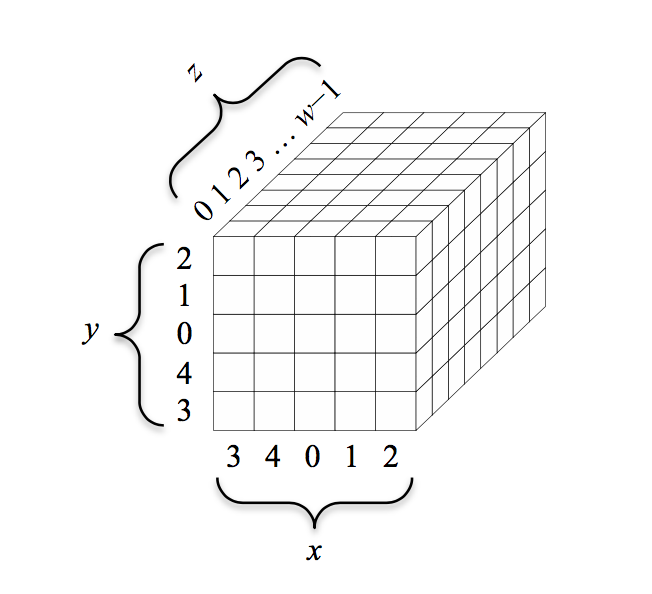
\includegraphics[width=0.55\textwidth]{chapters/pictures/keccak_state.png}
\caption[{Stanje permutacije Keccak-$f[1600]$}]{Stanje permutacije Keccak-$f[1600]$. Preuzeto iz \cite{keccak}}
\label{fig:keccak_stanje}
\end{figure}

Permutacija se sastoji od 24 runde, a svaka runda primenjuje redom pet koraka, $\theta$, $\rho$, $\pi$, $\chi$ i $\iota$, kako je prikazano na slici \ref{fig:keccak_runda}. Svi indeksi u nastavku računaju se po modulu 5, a $\mathrm{rot}(\cdot, k)$ označava cikličko pomeranje trake za $k$ bitova. U nastavku je svaki korak opisan pojedinačno.

\begin{figure}[H]
\centering
\resizebox{0.9\textwidth}{!}{
\begin{tikzpicture}
    \node (sin) [blokdata, minimum width=1.6cm] at (0,0) {$S_{\mathrm{ulaz}}$};
    \node (theta) [blokkripto, minimum width=1.2cm] at (2.2,0) {$\theta$};
    \node (rho) [blokkripto, minimum width=1.2cm] at (3.9,0) {$\rho$};
    \node (pi) [blokkripto, minimum width=1.2cm] at (5.6,0) {$\pi$};
    \node (chi) [blokkripto, minimum width=1.2cm] at (7.3,0) {$\chi$};
    \node (iota) [blokkripto, minimum width=1.2cm] at (9.0,0) {$\iota$};
    \node (sout) [blokrezultat, minimum width=1.6cm] at (11.2,0) {$S_{\mathrm{izlaz}}$};
    \draw [strelica] (sin) -- (theta);
    \draw [strelica] (theta) -- (rho);
    \draw [strelica] (rho) -- (pi);
    \draw [strelica] (pi) -- (chi);
    \draw [strelica] (chi) -- (iota);
    \draw [strelica] (iota) -- (sout);
\end{tikzpicture}
}
\caption{Jedna runda permutacije Keccak-$f[1600]$}
\label{fig:keccak_runda}
\end{figure}

\subsubsection{Korak \texorpdfstring{$\theta$}{theta}}

Korak $\theta$ je jedini koji meša bitove duž $y$-ose i time obezbeđuje difuziju između kolona. Za svako $x$ najpre se izračuna traka parnosti $C_x$, kao XOR svih pet traka sa tim $x$, pa se od parnosti dve susedne ravni formira korekcija $D_x$ i doda svim trakama ravni $x$:
\begin{align}
    C_x &= \bigoplus_{y=0}^{4} A_{x,y}, \qquad D_x = C_{x-1} \oplus \mathrm{rot}(C_{x+1}, 1), \nonumber\\
    A_{x,y} &\gets A_{x,y} \oplus D_x.
    \label{eq:keccak_theta}
\end{align}
Pošto je XOR bitska operacija, $C_x$ nije jedan bit nego cela traka od 64 bita. Njen bit na dubini $z$ jednak je parnosti onih pet bitova koji na toj dubini čine kolonu $(x,z)$. Dimenzija $z$ se pri tome ne meša, računa se 64 nezavisne parnosti, po jedna za svaku dubinu. Jedina operacija u ovom koraku koja uopšte pomera bitove duž $z$-ose jeste rotacija za jedno mesto u izrazu za $D_x$. Sve ostalo se odvija bit po bit, na istoj dubini.
\smallbreak
Ako se izraz (\ref{eq:keccak_theta}) raspiše na nivou pojedinačnog bita, dobija se
\begin{align}
    A_{x,y}[z] \;\gets\;\; & A_{x,y}[z] \nonumber\\[0.4ex]
    &\oplus\; \underbrace{\bigoplus_{y'=0}^{4} A_{x-1,\,y'}[z]}_{\text{parnost kolone } (x-1,\;z)} \nonumber\\[0.4ex]
    &\oplus\; \underbrace{\bigoplus_{y'=0}^{4} A_{x+1,\,y'}[z-1]}_{\text{parnost kolone } (x+1,\;z-1)},
\end{align}
gde $A_{x,y}[z]$ označava bit na dubini $z$ trake $A_{x,y}$.
Svaki izlazni bit zavisi, dakle, od jedanaest ulaznih, od sebe samog i od dve pune kolone. Isto važi i u suprotnom smeru, jer jedan ulazni bit ulazi u jedanaest izlaznih. Otuda brza difuzija, jer promena jednog jedinog bita stanja već posle nekoliko rundi zahvata celo stanje. Delovanje koraka po ravnima prikazano je na slici \ref{fig:keccak_theta}.
\smallbreak
U hardveru $\theta$ nosi najdužu kombinacionu putanju od pet koraka, ali je i ona plitka, jer je parnost XOR sa pet ulaza, koji staje u jedan šestoulazni LUT, pa je ceo korak dubok svega tri nivoa logike, parnosti kolona, korekcije $D_x$ i završnog XOR-a. Nema ni množenja ni tabela u memoriji.

\begin{figure}[H]
\centering
\resizebox{0.40\textwidth}{!}{
{\kvsetup
\begin{tabular}{|c|c|c|c|c|c|}
\hline
\rowcolor{gray!30}
\makebox[1cm]{} & \kv{$x{=}0$} & \kv{$x{=}1$} & \kv{$x{=}2$} & \kv{$x{=}3$} & \kv{$x{=}4$} \\
\hline
\cellcolor{gray!30}\kv{$y{=}0$} & \cellcolor{cyan!30}\kv{$A_{0,0}$} & \cellcolor{green!30}\kv{$A_{1,0}$} & \cellcolor{yellow!30}\kv{$A_{2,0}$} & \kv{$A_{3,0}$} & \kv{$A_{4,0}$} \\
\hline
\cellcolor{gray!30}\kv{$y{=}1$} & \cellcolor{cyan!30}\kv{$A_{0,1}$} & \cellcolor{green!30}\kv{$A_{1,1}$} & \cellcolor{yellow!30}\kv{$A_{2,1}$} & \kv{$A_{3,1}$} & \kv{$A_{4,1}$} \\
\hline
\cellcolor{gray!30}\kv{$y{=}2$} & \cellcolor{cyan!30}\kv{$A_{0,2}$} & \cellcolor{green!30}\kv{$A_{1,2}$} & \cellcolor{yellow!30}\kv{$A_{2,2}$} & \kv{$A_{3,2}$} & \kv{$A_{4,2}$} \\
\hline
\cellcolor{gray!30}\kv{$y{=}3$} & \cellcolor{cyan!30}\kv{$A_{0,3}$} & \cellcolor{green!30}\kv{$A_{1,3}$} & \cellcolor{yellow!30}\kv{$A_{2,3}$} & \kv{$A_{3,3}$} & \kv{$A_{4,3}$} \\
\hline
\cellcolor{gray!30}\kv{$y{=}4$} & \cellcolor{cyan!30}\kv{$A_{0,4}$} & \cellcolor{green!30}\kv{$A_{1,4}$} & \cellcolor{yellow!30}\kv{$A_{2,4}$} & \kv{$A_{3,4}$} & \kv{$A_{4,4}$} \\
\hline
\end{tabular}
}}
\caption{Korak $\theta$ za ravan $x=1$ -- svaka traka ravni (zeleno) sabira se sa trakom parnosti ravni $x=0$ (cijan) i rotiranom trakom parnosti ravni $x=2$ (žuto)}
\label{fig:keccak_theta}
\end{figure}

\subsubsection{Korak \texorpdfstring{$\rho$}{rho}}

Korak $\rho$ ciklično rotira svaku traku za njen fiksni ofset:
\begin{equation}
    A_{x,y} \gets \mathrm{rot}\big(A_{x,y},\, r_{x,y}\big),
\end{equation}
gde su $r_{x,y}$ konstante definisane standardom, date u dodatku \ref{app:keccak}. Rotacija premešta bitove unutar trake (duž $z$-ose stanja), čime difuzija iz koraka $\theta$, koja deluje po kolonama, dobija i treću dimenziju. Delovanje na jednu traku prikazano je na slici \ref{fig:keccak_rho}. U hardveru su ove rotacije fiksne i svode se na preusmeravanje veza, pa ne troše logiku.

\begin{figure}[H]
\centering
\resizebox{0.58\textwidth}{!}{
{\kvsetup
\begin{tabular}{c}
    \begin{tabular}{|c|c|c|c|c|c|c|c|}
    \hline
    \kv{$a_7$} & \kv{$a_6$} & \kv{$a_5$} & \kv{$a_4$} & \kv{$a_3$} & \cellcolor{green!30}\kv{$a_2$} & \cellcolor{green!30}\kv{$a_1$} & \cellcolor{green!30}\kv{$a_0$} \\
    \hline
    \end{tabular}
    \\[2ex]
    $\Big\downarrow\;\mathrm{rot}(\cdot,\,3)$
    \\[2ex]
    \begin{tabular}{|c|c|c|c|c|c|c|c|}
    \hline
    \kv{$a_4$} & \kv{$a_3$} & \cellcolor{green!30}\kv{$a_2$} & \cellcolor{green!30}\kv{$a_1$} & \cellcolor{green!30}\kv{$a_0$} & \kv{$a_7$} & \kv{$a_6$} & \kv{$a_5$} \\
    \hline
    \end{tabular}
\end{tabular}
}}
\caption[Korak $\rho$: ciklična rotacija trake]{Korak $\rho$: ciklična rotacija trake, prikazana na skraćenoj traci od 8 bitova za ofset 3. Tri istaknuta bita prelaze sa desnog kraja na poziciju tri mesta levlje. Bitovi koji izađu sa levog kraja ulaze sa desnog}
\label{fig:keccak_rho}
\end{figure}

\subsubsection{Korak \texorpdfstring{$\pi$}{pi}}

Korak $\pi$ premešta trake na nove pozicije u $5 \times 5$ matrici:
\begin{equation}
    A'_{\,y,\;(2x+3y) \bmod 5} \gets A_{x,y}.
\end{equation}
Dok $\rho$ meša bitove unutar traka, $\pi$ meša same trake između vrsta i kolona, čime se sprečava da se difuzija zadrži u lokalnim šablonima. Preslikavanje svih 25 traka prikazano je na slici \ref{fig:keccak_pi}. Iz izraza za odredište vidi se pravilnost koju slika čini očiglednom. Prvi indeks odredišta je $y$, pa sve trake jedne vrste polaznog stanja završavaju u istoj koloni novog stanja. Korak $\pi$ je, dakle, transpozicija propraćena preslikavanjem $x \mapsto 2x + 3y$ unutar kolone. Traka $A_{0,0}$ jedina ostaje na svom mestu, a duž prve vrste novog stanja poređala se dijagonala polaznog. I ovaj korak je u hardveru besplatan. Kao i ShiftRows transformacija AES algoritma, o kojoj će biti reči u odeljku \ref{subsec:aes_transformacije}, i ovde je reč o čistom preusmeravanju veza.

\begin{figure}[H]
\centering
\resizebox{\textwidth}{!}{
{\kvsetup
\begin{tabular}{c c c}
    \begin{tabular}{|c|c|c|c|c|c|}
    \hline
    \rowcolor{gray!30}
    \makebox[1cm]{} & \kv{$x{=}0$} & \kv{$x{=}1$} & \kv{$x{=}2$} & \kv{$x{=}3$} & \kv{$x{=}4$} \\
    \hline
    \cellcolor{gray!30}\kv{$y{=}0$} & \cellcolor{green!30}\kv{$A_{0,0}$} & \cellcolor{green!30}\kv{$A_{1,0}$} & \cellcolor{green!30}\kv{$A_{2,0}$} & \cellcolor{green!30}\kv{$A_{3,0}$} & \cellcolor{green!30}\kv{$A_{4,0}$} \\
    \hline
    \cellcolor{gray!30}\kv{$y{=}1$} & \cellcolor{yellow!30}\kv{$A_{0,1}$} & \cellcolor{yellow!30}\kv{$A_{1,1}$} & \cellcolor{yellow!30}\kv{$A_{2,1}$} & \cellcolor{yellow!30}\kv{$A_{3,1}$} & \cellcolor{yellow!30}\kv{$A_{4,1}$} \\
    \hline
    \cellcolor{gray!30}\kv{$y{=}2$} & \cellcolor{cyan!30}\kv{$A_{0,2}$} & \cellcolor{cyan!30}\kv{$A_{1,2}$} & \cellcolor{cyan!30}\kv{$A_{2,2}$} & \cellcolor{cyan!30}\kv{$A_{3,2}$} & \cellcolor{cyan!30}\kv{$A_{4,2}$} \\
    \hline
    \cellcolor{gray!30}\kv{$y{=}3$} & \cellcolor{purple!30}\kv{$A_{0,3}$} & \cellcolor{purple!30}\kv{$A_{1,3}$} & \cellcolor{purple!30}\kv{$A_{2,3}$} & \cellcolor{purple!30}\kv{$A_{3,3}$} & \cellcolor{purple!30}\kv{$A_{4,3}$} \\
    \hline
    \cellcolor{gray!30}\kv{$y{=}4$} & \cellcolor{orange!30}\kv{$A_{0,4}$} & \cellcolor{orange!30}\kv{$A_{1,4}$} & \cellcolor{orange!30}\kv{$A_{2,4}$} & \cellcolor{orange!30}\kv{$A_{3,4}$} & \cellcolor{orange!30}\kv{$A_{4,4}$} \\
    \hline
    \end{tabular}
    &
    \raisebox{-16ex}{\Huge $\;\longrightarrow\;$}
    &
    \begin{tabular}{|c|c|c|c|c|c|}
    \hline
    \rowcolor{gray!30}
    \makebox[1cm]{} & \kv{$x{=}0$} & \kv{$x{=}1$} & \kv{$x{=}2$} & \kv{$x{=}3$} & \kv{$x{=}4$} \\
    \hline
    \cellcolor{gray!30}\kv{$y{=}0$} & \cellcolor{green!30}\kv{$A_{0,0}$} & \cellcolor{yellow!30}\kv{$A_{1,1}$} & \cellcolor{cyan!30}\kv{$A_{2,2}$} & \cellcolor{purple!30}\kv{$A_{3,3}$} & \cellcolor{orange!30}\kv{$A_{4,4}$} \\
    \hline
    \cellcolor{gray!30}\kv{$y{=}1$} & \cellcolor{green!30}\kv{$A_{3,0}$} & \cellcolor{yellow!30}\kv{$A_{4,1}$} & \cellcolor{cyan!30}\kv{$A_{0,2}$} & \cellcolor{purple!30}\kv{$A_{1,3}$} & \cellcolor{orange!30}\kv{$A_{2,4}$} \\
    \hline
    \cellcolor{gray!30}\kv{$y{=}2$} & \cellcolor{green!30}\kv{$A_{1,0}$} & \cellcolor{yellow!30}\kv{$A_{2,1}$} & \cellcolor{cyan!30}\kv{$A_{3,2}$} & \cellcolor{purple!30}\kv{$A_{4,3}$} & \cellcolor{orange!30}\kv{$A_{0,4}$} \\
    \hline
    \cellcolor{gray!30}\kv{$y{=}3$} & \cellcolor{green!30}\kv{$A_{4,0}$} & \cellcolor{yellow!30}\kv{$A_{0,1}$} & \cellcolor{cyan!30}\kv{$A_{1,2}$} & \cellcolor{purple!30}\kv{$A_{2,3}$} & \cellcolor{orange!30}\kv{$A_{3,4}$} \\
    \hline
    \cellcolor{gray!30}\kv{$y{=}4$} & \cellcolor{green!30}\kv{$A_{2,0}$} & \cellcolor{yellow!30}\kv{$A_{3,1}$} & \cellcolor{cyan!30}\kv{$A_{4,2}$} & \cellcolor{purple!30}\kv{$A_{0,3}$} & \cellcolor{orange!30}\kv{$A_{1,4}$} \\
    \hline
    \end{tabular}
\end{tabular}
}
}
\caption[Korak $\pi$: preslikavanje svih 25 traka]{Korak $\pi$: preslikavanje svih 25 traka. Levo je polazno, desno novo stanje. U svakoj ćeliji novog stanja upisana je traka koja je na to mesto došla, a boja prati polaznu vrstu $y$}
\label{fig:keccak_pi}
\end{figure}

\subsubsection{Korak \texorpdfstring{$\chi$}{chi}}

Korak $\chi$ je jedina nelinearna operacija permutacije, analogon S-boksa AES algoritma, o kome će biti reči u odeljku \ref{subsec:aes_transformacije}, ali izuzetno jeftin. Deluje po vrstama stanja, dakle za fiksno $y$, tako što se svaka traka sabira sa proizvodom komplementa prve i vrednosti druge naredne trake u istoj vrsti:
\begin{equation}
    A_{x,y} \gets A_{x,y} \oplus \big(\overline{A_{x+1,y}} \wedge A_{x+2,y}\big).
\end{equation}
Operacija je bitska. Logička mreža sa slike \ref{fig:keccak_chi} deluje na svaki od 64 bita trake nezavisno i paralelno, pa se u hardveru sastoji od 1600 identičnih kopija jednog NOT, jednog AND i jednog XOR kola, što je ekvivalent nelinearne supstitucije nad svih 1600 bitova stanja odjednom, bez ijedne memorijske tabele.

\begin{figure}[H]
\centering
\resizebox{0.75\textwidth}{!}{
\begin{tikzpicture}
    \node (a0) [blokdata, minimum width=2.1cm] at (0,0) {$A_{x,y}$};
    \node (a1) [blokdata, minimum width=2.1cm] at (0,-1.3) {$A_{x{+}1,y}$};
    \node (a2) [blokdata, minimum width=2.1cm] at (0,-2.6) {$A_{x{+}2,y}$};
    \node (inv) [circle, draw=black, thick, inner sep=2pt] at (2.7,-1.3) {$\lnot$};
    \node (and) [circle, draw=black, thick, inner sep=2pt] at (4.2,-1.95) {$\wedge$};
    \node (xor) [circle, draw=black, thick, inner sep=2pt] at (5.7,0) {$\oplus$};
    \node (out) [blokrezultat, minimum width=2.3cm] at (7.9,0) {$A'_{x,y}$};
    \draw [strelica] (a1) -- (inv);
    \draw [strelica] (inv) -| (and);
    \draw [strelica] (a2) -| (and);
    \draw [strelica] (a0) -- (xor);
    \draw [strelica] (and) -| (xor);
    \draw [strelica] (xor) -- (out);
\end{tikzpicture}
}
\caption{Korak $\chi$: logika za jednu traku}
\label{fig:keccak_chi}
\end{figure}

\subsubsection{Korak \texorpdfstring{$\iota$}{iota}}

Poslednji korak runde sabira konstantu runde sa jednom jedinom trakom:
\begin{equation}
    A_{0,0} \gets A_{0,0} \oplus RC_i,
\end{equation}
gde je $RC_i$ konstanta runde $i$, definisana standardom (sve 24 vrednosti date su u dodatku \ref{app:keccak}). Bez ovog koraka sve runde bile bi identične, pa bi permutacija imala simetrije koje Oskar može iskoristiti. Konstante, različite u svakoj rundi, tu simetriju narušavaju, a delovanje je prikazano na slici \ref{fig:keccak_iota}.

\begin{figure}[H]
\centering
\begin{tikzpicture}
    \node (a00) [blokdata, minimum width=2.2cm] {$A_{0,0}$};
    \node (xor) [circle, draw=black, thick, right=1.5cm of a00, inner sep=2pt] {$\oplus$};
    \node (rc) [rectangle, rounded corners, draw=black, fill=gray!30, minimum width=2cm, minimum height=0.9cm, above=1cm of xor] {$RC_i$};
    \node (out) [blokrezultat, minimum width=2.2cm, right=1.5cm of xor] {$A'_{0,0}$};
    \draw [strelica] (a00) -- (xor);
    \draw [strelica] (rc) -- (xor);
    \draw [strelica] (xor) -- (out);
\end{tikzpicture}
\caption{Korak $\iota$}
\label{fig:keccak_iota}
\end{figure}
\smallbreak
Sa stanovišta hardverske realizacije, presudno je da se svi koraci svode na bitske operacije XOR, AND, NOT i fiksne rotacije, pri čemu fiksne rotacije u hardveru ne koštaju ništa. Jedna runda je stoga plitka kombinaciona mreža, a cela permutacija se prirodno realizuje iterativno, sa jednom rundom po taktu.

\subsection{Varijante standarda}
\label{subsec:sha3_varijante}

FIPS 202 definiše četiri heš funkcije fiksnog izlaza i dve XOF funkcije, sve nad istom permutacijom Keccak-$f[1600]$, a međusobno različite samo po brzini $r$, kapacitetu $c$ i dužini izlaza, kako je dato u tabeli \ref{tab:sha3_varijante}.

\begin{table}[H]
\caption[Varijante SHA-3 standarda]{Varijante SHA-3 standarda \cite{fips202}}
\centering
\resizebox{0.9\textwidth}{!}{
\begin{tabular}{|c|c|c|c|c|c|}
\hline
\rowcolor{gray!30}
\rsz[2.4cm]{1.2}{Funkcija} & \rsz[1.6cm]{1.2}{$r$ [bit]} & \rsz[1.6cm]{1.2}{$c$ [bit]} & \rsz[2.4cm]{1.2}{Izlaz $d$ [bit]} & \rsz[2.8cm]{1.2}{Kolizije [bit]} & \rsz[2.8cm]{1.2}{Original [bit]} \\
\hline
\rsz[2.2cm]{1.2}{SHA3-224} & \rsz[1cm]{1.2}{1152} & \rsz[1cm]{1.2}{448} & \rsz[1.4cm]{1.2}{224} & \rsz[1.4cm]{1.2}{112} & \rsz[1.4cm]{1.2}{224} \\
\hline
\rsz[2.2cm]{1.2}{SHA3-256} & \rsz[1cm]{1.2}{1088} & \rsz[1cm]{1.2}{512} & \rsz[1.4cm]{1.2}{256} & \rsz[1.4cm]{1.2}{128} & \rsz[1.4cm]{1.2}{256} \\
\hline
\rsz[2.2cm]{1.2}{SHA3-384} & \rsz[1cm]{1.2}{832} & \rsz[1cm]{1.2}{768} & \rsz[1.4cm]{1.2}{384} & \rsz[1.4cm]{1.2}{192} & \rsz[1.4cm]{1.2}{384} \\
\hline
\rsz[2.2cm]{1.2}{SHA3-512} & \rsz[1cm]{1.2}{576} & \rsz[1cm]{1.2}{1024} & \rsz[1.4cm]{1.2}{512} & \rsz[1.4cm]{1.2}{256} & \rsz[1.4cm]{1.2}{512} \\
\hline
\rsz[2.2cm]{1.2}{SHAKE128} & \rsz[1cm]{1.2}{1344} & \rsz[1cm]{1.2}{256} & \rsz[2.2cm]{1.2}{proizvoljan} & \rsz[2.4cm]{1.2}{$\min(d/2,\,128)$} & \rsz[2.4cm]{1.2}{$\min(d,\,128)$} \\
\hline
\rsz[2.2cm]{1.2}{SHAKE256} & \rsz[1cm]{1.2}{1088} & \rsz[1cm]{1.2}{512} & \rsz[2.2cm]{1.2}{proizvoljan} & \rsz[2.4cm]{1.2}{$\min(d/2,\,256)$} & \rsz[2.4cm]{1.2}{$\min(d,\,256)$} \\
\hline
\end{tabular}
}
\label{tab:sha3_varijante}
\end{table}

Činjenica da sve varijante dele istu permutaciju izuzetno je povoljna za hardver, jer je jedno jezgro permutacije dovoljno za ceo standard, a varijanta se bira samo upravljačkom logikom koja određuje koliko se bitova stanja puni, odnosno čita. Uočava se i prirodan kompromis. Varijante sa većim kapacitetom pružaju veću sigurnost, ali obrađuju manje bitova poruke po pozivu permutacije, dakle imaju manju propusnost.

\subsection{Izvedene funkcije: cSHAKE i KMAC}
\label{subsec:kmac}

Nad istom sponge konstrukcijom NIST je standardom SP 800-185 \cite{sp800185} definisao familiju izvedenih funkcija (engl. \textit{derived functions}), od kojih su za ovaj rad značajne cSHAKE i KMAC.
\smallbreak
\textit{cSHAKE} (engl. \textit{customizable SHAKE}) proširuje SHAKE funkcije sa dva dodatna parametra: imenom funkcije $N$, rezervisanim za NIST-ove definicije, i oznakom namene (engl. \textit{customization string}) $S$, kojom korisnik razdvaja različite upotrebe iste funkcije. Parametri se kodiraju u prefiksni blok od jednog ili više celih $r$-bitnih blokova (za ime i oznaku namene iz ovog rada tačno jedan), koji se upija pre same poruke, a sufiks za razdvajanje domena iz tabele \ref{tab:sha3_domeni} menja se u \texttt{00} umesto \texttt{1111} kod SHAKE funkcija, dakle u bajt \texttt{0x04} umesto \texttt{0x1F}.
\smallbreak
Slučaj kada su i $N$ i $S$ prazni standard uređuje posebnim pravilom, a ne kao posledicu konstrukcije. Tada je po definiciji $\mathrm{cSHAKE}(X, L, \texttt{""}, \texttt{""}) = \mathrm{SHAKE}(X, L)$ \cite{sp800185}. To znači da se u tom slučaju prefiksni blok uopšte ne formira i da se koristi SHAKE sufiks \texttt{1111}, dakle bajt \texttt{0x1F}. Bez tog izuzetka cSHAKE sa praznim parametrima ne bi davao isti izlaz kao SHAKE, upravo zato što bi sufiks bio drugačiji.
\smallbreak
Pre same definicije KMAC funkcije potrebne su četiri pomoćne funkcije kodiranja iz standarda \cite{sp800185}. Parametri koji ulaze u konstrukciju dve su vrste: brojevi (dužine) i stringovi (ime funkcije, oznaka namene, ključ), a ove četiri funkcije ih prevode u zapis iz koga se svaki sastavni deo može jednoznačno pročitati. Time se sprečava da dva različita skupa parametara daju isti ulazni niz. Sve četiri sažeto su date u tabeli \ref{tab:sp800185_kodiranja}.

\begin{table}[H]
\caption[Pomoćne funkcije kodiranja iz standarda SP 800-185]{Pomoćne funkcije kodiranja iz standarda SP 800-185 \cite{sp800185}}
\centering
\resizebox{\textwidth}{!}{
\begin{tabular}{|c|c|c|}
\hline
\rowcolor{gray!30}
\rsz[4cm]{1.2}{Funkcija} & \rsz[7cm]{1.2}{Rezultat} & \rsz[7cm]{1.2}{Uloga} \\
\hline
\rsz[4.4cm]{1.2}{$\mathrm{left\_encode}(x)$} & \makecell{\rsz[6.6cm]{1.2}{dužina zapisa, pa sam broj $x$} \\ \rsz[6.6cm]{1.2}{(brojač dužine ispred)}} & \rsz[7cm]{1.2}{dužina koja prethodi podatku} \\
\hline
\rsz[4.4cm]{1.2}{$\mathrm{right\_encode}(x)$} & \makecell{\rsz[6.6cm]{1.2}{broj $x$, pa dužina zapisa} \\ \rsz[6.6cm]{1.2}{(brojač dužine iza)}} & \rsz[7cm]{1.2}{dužina koja sledi iza podatka} \\
\hline
\rsz[4.4cm]{1.2}{$\mathrm{encode\_string}(S)$} & \rsz[6.6cm]{1.2}{$\mathrm{left\_encode}(\mathrm{len}(S)) \,\|\, S$} & \rsz[7cm]{1.2}{string kome prethodi dužina} \\
\hline
\rsz[4.4cm]{1.2}{$\mathrm{bytepad}(X, w)$} & \makecell{\rsz[6.6cm]{1.2}{$\mathrm{left\_encode}(w) \,\|\, X$, dopunjeno} \\ \rsz[6.6cm]{1.2}{nulama do umnoška $w$ bajtova}} & \rsz[7cm]{1.2}{poravnanje na granicu bloka} \\
\hline
\end{tabular}
}
\label{tab:sp800185_kodiranja}
\end{table}

Dve varijante zapisa dužine postoje zbog dva različita mesta na kojima zapis stoji. Kada dužina prethodi podatku, čitalac je pročita pa zna koliko bajtova posle nje da uzme. Tako rade prefiksni blok i blok ključa, iza kojih sledi još sadržaja. Kodirana dužina izlaza, međutim, stoji na samom kraju ulaznog niza, iza poruke čija dužina unapred nije poznata, pa se do nje dolazi čitanjem sa kraja. Poslednji bajt kaže koliko bajtova broja stoji ispred njega, pa ona zato koristi $\mathrm{right\_encode}$.
\smallbreak
\textit{KMAC} (engl. \textit{Keccak Message Authentication Code}) je funkcija sa tajnim ključem izgrađena nad cSHAKE funkcijom sa imenom $N = \texttt{"KMAC"}$:
\begin{align}
    \mathrm{KMAC}[K, X, L, S] = \mathrm{cSHAKE}\big(
        &\mathrm{bytepad}(\mathrm{encode\_string}(K),\, r/8) \nonumber\\
        &\quad {}\,\|\, X \,\|\, \mathrm{right\_encode}(L), \nonumber\\
        &L,\; \texttt{"KMAC"},\; S\big),
    \label{eq:kmac}
\end{align}
gde se ključ $K$ kodira i dopuni u ceo blok koji se upija pre poruke $X$, a $\mathrm{right\_encode}(L)$ na kraj poruke dodaje kodiranu dužinu izlaza $L$ (varijanta KMACXOF, sa $\mathrm{right\_encode}(0)$, daje izlaz proizvoljne dužine u XOF režimu).
\smallbreak
Postavlja se pitanje zašto je posebna konstrukcija uopšte potrebna, kada sunđer nema svojstvo produženja poruke (odeljak \ref{subsec:sponge_sigurnost}), pa naivni oblik $H(K \,\|\, X)$ nad SHA-3 funkcijom nije ugrožen napadom koji kod Merkle--Damgardove klase nameće HMAC. KMAC ipak donosi tri svojstva koja taj oblik nema. Prva je kodiranje ključa sa dužinom upisanom ispred njega, čime granica ključa postaje deo samog niza, pa dva različita para ključa i poruke nikada ne daju isti ulaz. Druga je razdvajanje domena kroz ime $N$ i oznaku namene $S$, čime se isti ključ bezbedno koristi za više namena. Treća je kodirana dužina izlaza, čime skraćen izlaz nije prefiks dužeg. Rezultat je standardizovana pseudoslučajna funkcija (engl. \textit{pseudorandom function}, PRF) čija sigurnost počiva neposredno na kapacitetu sponge konstrukcije, odobrena i kao MAC i kao funkcija za izvođenje ključeva, i sve to jednim pozivom heš funkcije, bez dva ulančana poziva koja traži HMAC.
\smallbreak
Iako izraz (\ref{eq:kmac}) deluje glomazno, on ne uvodi nikakvo novo izračunavanje. Sve što opisuje jeste redosled kojim se polja nadovezuju u ulazni niz pre upijanja. Kako sastavljeni niz izgleda prikazuje slika \ref{fig:kmac_okvir}. Bitno je uočiti da su prva dva polja celi $r$-bitni blokovi. Prefiksni blok nosi ime funkcije i oznaku namene, a blok ključa je dopunjen funkcijom $\mathrm{bytepad}$ do granice bloka. Tek posle njih dolazi sama poruka, pa kodirana dužina izlaza, i na kraju dopuna iz odeljka \ref{subsec:sha3_dopuna} sa sufiksom \texttt{00}, jer je reč o cSHAKE funkciji.

\begin{figure}[H]
\centering
\setlength{\tabcolsep}{8pt}
\renewcommand{\arraystretch}{1.6}
\resizebox{\textwidth}{!}{
\begin{tabular}{|c|c|c|c|c|}
\multicolumn{1}{c}{ceo blok od $r$ bitova} & \multicolumn{1}{c}{ceo blok od $r$ bitova} & \multicolumn{3}{c}{} \\
\hline
\cellcolor{cyan!30}prefiksni blok $(N, S)$ & \cellcolor{purple!30}blok ključa $K$ & \cellcolor{green!30}poruka $X$ & \cellcolor{yellow!30}$\mathrm{right\_encode}(L)$ & \cellcolor{gray!30}dopuna \\
\hline
\end{tabular}
}
\caption[Uokvirivanje ulaznog niza KMAC funkcije]{Uokvirivanje ulaznog niza KMAC funkcije pre upijanja}
\label{fig:kmac_okvir}
\end{figure}

\begin{example}
\label{ex:kmac_bajtovi}
U ulozi koju KMAC256 ima u ovom radu, u izvođenju ključeva, ulogu ključa $K$ ima so (engl. \textit{salt}) od 32 bajta, poruka $X$ nosi zajedničku tajnu i kontekst razmene, ovde 72 bajta tajne i 40 bajtova konteksta, ukupno 112, oznaka namene $S$ je \texttt{"KDF"}, kako za ovu ulogu propisuje SP 800-56C \cite{sp80056c}, a dužina izlaza $L = 256$ bitova odgovara ključu za AES-256 (raspodela parametara data je u tabeli \ref{tab:kmac_uloge}). Brzina upijanja je $r/8 = 136$ bajtova, pa je $\mathrm{left\_encode}(136) = \texttt{01 88}$, i tim parom počinju oba uokvirena bloka:
\begin{center}
\small
\setlength{\tabcolsep}{6pt}
\renewcommand{\arraystretch}{1.3}
\begin{tabular}{|l|l|l|}
\hline
\rowcolor{gray!30}
Bajtovi & Zapis & Značenje \\
\hline
\cellcolor{cyan!30}\texttt{01 88} & $\mathrm{left\_encode}(136)$ & brzina upijanja $r/8$ \\
\hline
\cellcolor{cyan!30}\texttt{01 20} & $\mathrm{left\_encode}(32)$ & dužina imena, $4 \cdot 8$ bitova \\
\hline
\cellcolor{cyan!30}\texttt{4B 4D 41 43} & \texttt{"KMAC"} u ASCII zapisu & ime funkcije $N$ \\
\hline
\cellcolor{cyan!30}\texttt{01 18} & $\mathrm{left\_encode}(24)$ & dužina oznake, $3 \cdot 8$ bitova \\
\hline
\cellcolor{cyan!30}\texttt{4B 44 46} & \texttt{"KDF"} u ASCII zapisu & oznaka namene $S$ \\
\hline
\cellcolor{gray!30}\texttt{00} $\times\,123$ & dopuna nulama & do granice prvog bloka \\
\hline
\cellcolor{purple!30}\texttt{01 88} & $\mathrm{left\_encode}(136)$ & brzina upijanja $r/8$ \\
\hline
\cellcolor{purple!30}\texttt{02 01 00} & $\mathrm{left\_encode}(256)$ & dužina ključa, $32 \cdot 8$ bitova \\
\hline
\cellcolor{purple!30}$K$, 32 bajta & --- & so, u ulozi ključa \\
\hline
\cellcolor{gray!30}\texttt{00} $\times\,99$ & dopuna nulama & do granice drugog bloka \\
\hline
\cellcolor{green!30}$X$, 112 bajtova & --- & zajednička tajna i kontekst razmene \\
\hline
\cellcolor{yellow!30}\texttt{01 00 02} & $\mathrm{right\_encode}(256)$ & dužina izlaza $L$ \\
\hline
\cellcolor{gray!30}\texttt{04 00 \dots\ 00 80} & sufiks i dopuna & do granice trećeg bloka \\
\hline
\end{tabular}
\end{center}
Dužine stringova izražene su u bitovima, ne u bajtovima, pa ime od četiri znaka daje \texttt{0x20}, a so od 32 bajta vrednost 256, koja se više ne smešta u jedan bajt. U ovom primeru se, sasvim nezavisno od toga, i za dužinu izlaza slučajno bira istih 256 bitova, a mogla je biti i drugačija. Baš zato što je broj isti, na njegova dva zapisa vidi se razlika iz tabele \ref{tab:sp800185_kodiranja}. Zapis \texttt{02 01 00} u bloku ključa čita se unapred, sa brojem bajtova ispred, a \texttt{01 00 02} na kraju niza unazad, sa brojem bajtova iza.
\end{example}

Primer pokazuje i donju granicu cene. Prefiksni blok i blok ključa su celi blokovi bez obzira na to koliko su $N$, $S$ i $K$ kratki, a poruka sa kodiranom dužinom izlaza i završnom dopunom traži bar još jedan, pa KMAC nikada ne košta manje od tri poziva permutacije, ni kada su svi parametri prazni. Kod kratkih ulaza, kakvi se u izvođenju ključeva i javljaju, dva od ta tri bloka nose samo okvir. Isti raspored donosi i pogodnost. Poruka $X$ uvek počinje na poznatoj granici bloka, kod KMAC256 posle tačno 272 bajta okvira, pa strana koja ulazni niz sastavlja upisuje unapred poznate bajtove na unapred poznata mesta i ne mora da prati pomeraj unutar bloka.
\smallbreak
Raspodela parametara iz primera \ref{ex:kmac_bajtovi} upravo je ona koju KMAC ima u hibridnom sistemu iz odeljka \ref{sec:hibridni_sistem}, a to je izvođenje ključeva po jednokoračnoj KDF šemi iz NIST preporuke SP 800-56C \cite{sp80056c}. Ona nije ista kao pri upotrebi za autentifikaciju poruka, a razliku uporedno prikazuje tabela \ref{tab:kmac_uloge}. Suština je u tome što se tajnost seli iz ključa u poruku. Zajednička tajna $Z$ dobijena ECDH razmenom ulazi u poruku $X$, nadovezana sa fiksnim kontekstom razmene (engl. \textit{FixedInfo}), koji obuhvata identitete strana i oznaku protokola, dok je ključ $K$ so, koja po standardu sme biti i unapred dogovorena javna vrednost. Oznaku namene $S$ standard pritom fiksira na vrednost \texttt{"KDF"}, čime je upotreba KMAC-a za izvođenje ključeva razdvojena od svih ostalih upotreba iste funkcije. Ključ sesije i inicijalne vrednosti seku se iz jednog izlaza tražene dužine, a njihov kontekst nosi FixedInfo.

\begin{table}[H]
\caption{Uloge parametara KMAC funkcije: autentifikacija poruka naspram izvođenja ključeva}
\centering
\resizebox{\textwidth}{!}{
\begin{tabular}{|c|c|c|}
\hline
\rowcolor{gray!30}
\rsz[3.4cm]{1.2}{Parametar} & \rsz[6.6cm]{1.2}{KMAC kao MAC} & \rsz[7.4cm]{1.2}{KMAC kao KDF (SP 800-56C)} \\
\hline
\rsz[3cm]{1.2}{ključ $K$} & \rsz[6.2cm]{1.2}{tajni ključ koji strane dele} & \rsz[7cm]{1.2}{so, sme biti i javna vrednost} \\
\hline
\rsz[3cm]{1.2}{poruka $X$} & \rsz[6.2cm]{1.2}{podatak koji se autentifikuje} & \rsz[7cm]{1.2}{$Z \,\|\, \mathrm{FixedInfo}$, tajna je u $Z$} \\
\hline
\rsz[3cm]{1.2}{oznaka $S$} & \rsz[6.2cm]{1.2}{razdvajanje namena istog ključa} & \rsz[7cm]{1.2}{standard je fiksira na \texttt{"KDF"}} \\
\hline
\rsz[3cm]{1.2}{izlaz} & \rsz[6.2cm]{1.2}{autentifikaciona oznaka} & \rsz[7cm]{1.2}{ključni materijal} \\
\hline
\end{tabular}
}
\label{tab:kmac_uloge}
\end{table}

U radu je korišćen KMAC256. Ovim izborom ceo lanac pokriven je NIST standardima: uspostavljanje zajedničke tajne po SP 800-56A \cite{sp80056a}, izvođenje ključeva po SP 800-56C \cite{sp80056c}, a zaštita saobraćaja po SP 800-38D \cite{sp80038d}.
\smallbreak
Celokupno KMAC uokvirivanje, dakle prefiksni blok, blok ključa i kodirana dužina izlaza, jeste čisto formatiranje ulaznog niza, jer nijedan od tih koraka ne dira permutaciju niti stanje sunđera. Za KMAC je zato dovoljna svaka realizacija cSHAKE funkcije. Kako je to iskorišćeno u akceleratoru opisano je u odeljku \ref{subsec:hw_sha3_kmac}.

\section{AES-GCM}
\label{sec:aes_gcm}

Treću komponentu sistema čini AES u GCM režimu rada, algoritam za simetrično šifrovanje kojim se štiti korisnički saobraćaj. U ovom odeljku najpre je opisan sam AES algoritam, njegova arhitektura, transformacije u rundi i ekspanzija ključa, a zatim GCM režim koji od blok šifre gradi autentifikovano šifrovanje. Detaljna analiza AES algoritma, sa kompletnim matematičkim osnovama i izvođenjima nad poljem $\mathrm{GF}(2^8)$, data je u \cite{gavrilovic_diplomski}.
\smallbreak
Izlaganje prati notaciju standarda \cite{fips197, sp80038d} uz jedno odstupanje. Otvoreni tekst, šifrat, autentifikaciona oznaka i pridruženi podaci (engl. \textit{Additional Authenticated Data}) označeni su sa $\mathrm{PT}$, $\mathrm{CT}$, $\mathrm{ICV}$ i $\mathrm{AAD}$, umesto sa $P$, $C$, $T$ i $A$. Razlog je dvostruk. Takve oznake prate uobičajenu terminologiju mrežnih protokola, a simboli $T$ i $A$ su već zauzeti: $T$ za T-tabele u odeljku \ref{subsec:aes_ttabele}, a $A$ za stanje Keccak permutacije i operande množenja.

\subsection{Nastanak standarda}
\label{subsec:aes_istorijat}

NIST je 1997. godine raspisao javni konkurs za novi standard šifrovanja, kao zamenu za zastareli DES čija je dužina ključa od 56 bitova postala nedovoljna pred rastućom računarskom snagom. Nakon dve runde svetske evaluacije, u kojima su kandidati ocenjivani po sigurnosti, brzini u softveru i hardveru i jednostavnosti realizacije, za pobednika je 2000. godine proglašen algoritam Rijndael belgijskih kriptografa Joana Daemena i Vincenta Rijmena \cite{daemen_rijndael}. Standardizovana verzija, objavljena 2001. godine kao FIPS 197 \cite{fips197}, sužava fleksibilnost izvornog algoritma. Dužina bloka fiksirana je na 128 bitova, a dozvoljene dužine ključa su 128, 192 i 256 bitova, po kojima varijante nose nazive AES-128, AES-192 i AES-256.

\subsection{Arhitektura algoritma}
\label{subsec:aes_arhitektura}

AES obrađuje blok od 128 bitova predstavljen kao matrica $4 \times 4$ bajtova, koja se naziva matrica stanja (engl. \textit{state}). Bajtovi ulaznog bloka pune matricu po kolonama, a svaka transformacija algoritma ažurira stanje novim vrednostima. Broj kolona matrice stanja označava se sa $N_b$ i za AES iznosi $N_b = 128/32 = 4$. Raspored bajtova u matrici prikazan je na slici \ref{fig:aes_matrica_stanja}.

\begin{figure}[H]
\centering
\resizebox{0.30\textwidth}{!}{
{\kvsetup
\begin{tabular}{|c|c|c|c|}
\hline
\kv{$s_{0,0}$} & \kv{$s_{0,1}$} & \kv{$s_{0,2}$} & \kv{$s_{0,3}$} \\
\hline
\kv{$s_{1,0}$} & \kv{$s_{1,1}$} & \kv{$s_{1,2}$} & \kv{$s_{1,3}$} \\
\hline
\kv{$s_{2,0}$} & \kv{$s_{2,1}$} & \kv{$s_{2,2}$} & \kv{$s_{2,3}$} \\
\hline
\kv{$s_{3,0}$} & \kv{$s_{3,1}$} & \kv{$s_{3,2}$} & \kv{$s_{3,3}$} \\
\hline
\end{tabular}
}}
\caption{Matrica stanja AES algoritma}
\label{fig:aes_matrica_stanja}
\end{figure}

Svaki bajt matrice stanja tumači se kao element polja $\mathrm{GF}(2^8)$ sa redukcionim polinomom:
\begin{equation}
    m(x) = x^8 + x^4 + x^3 + x + 1,
    \label{eq:aes_polinom}
\end{equation}
pa su sve operacije nad bajtovima zapravo operacije u tom polju. Sabiranje je XOR, a množenje se izvodi po modulu $m(x)$. Analogno matrici stanja, ključ se predstavlja matricom od $N_k$ kolona, gde je $N_k$ dužina ključa podeljena sa 32. Broj rundi $N_r$ zavisi od dužine ključa, kako je prikazano u tabeli \ref{tab:aes_varijante}.

\begin{table}[H]
\caption[Varijante AES algoritma]{Varijante AES algoritma \cite{fips197}}
\centering
\resizebox{0.75\textwidth}{!}{
\begin{tabular}{|c|c|c|c|}
\hline
\rowcolor{gray!30}
\rsz[2.6cm]{1.2}{Varijanta} & \rsz[4.2cm]{1.2}{Dužina ključa [bit]} & \rsz[1.2cm]{1.2}{$N_k$} & \rsz[1.2cm]{1.2}{$N_r$} \\
\hline
\rsz[2.2cm]{1.2}{AES-128} & \rsz[1.4cm]{1.2}{128} & \rsz[0.8cm]{1.2}{4} & \rsz[0.8cm]{1.2}{10} \\
\hline
\rsz[2.2cm]{1.2}{AES-192} & \rsz[1.4cm]{1.2}{192} & \rsz[0.8cm]{1.2}{6} & \rsz[0.8cm]{1.2}{12} \\
\hline
\rsz[2.2cm]{1.2}{AES-256} & \rsz[1.4cm]{1.2}{256} & \rsz[0.8cm]{1.2}{8} & \rsz[0.8cm]{1.2}{14} \\
\hline
\end{tabular}
}
\label{tab:aes_varijante}
\end{table}

U ovom radu korišćen je AES-256.

\subsection{Tok šifrovanja}
\label{subsec:aes_tok}

Šifrovanje počinje početnom operacijom AddRoundKey, kojom se ulazni blok sabira sa prvim ključem runde operacijom XOR. Zatim sledi $N_r$ rundi, od kojih svaka primenjuje redom četiri transformacije: SubBytes, ShiftRows, MixColumns i AddRoundKey, s tim što se u poslednjoj rundi transformacija MixColumns izostavlja. Svaka runda koristi svoj ključ, dobijen postupkom ekspanzije ključa opisanim u odeljku \ref{subsec:aes_ekspanzija}.
\smallbreak
Svaka od četiri transformacije ima jasno odvojenu ulogu, a raspoređene su po klasičnoj podeli na konfuziju i difuziju:
\begin{itemize}[itemsep=2pt]
    \item SubBytes je nosilac konfuzije i jedina nelinearna operacija u algoritmu. Bez nje bi ceo AES bio linearno preslikavanje, pa i trivijalno rešiv.
    \item ShiftRows i MixColumns zajedno čine linearni sloj, zadužen za difuziju. MixColumns meša četiri bajta unutar kolone, dok ShiftRows ne kombinuje nijedan bajt sa drugim, nego ih samo premešta tako da bajtovi jedne vrste završe u različitim kolonama.
    \item AddRoundKey unosi tajni materijal ključa u stanje. I ona je linearna operacija i sama ne doprinosi ni konfuziji ni difuziji. Njena je uloga da nelinearnost naredne runde ima na šta da deluje.
\end{itemize}
Podela posla unutar linearnog sloja objašnjava zašto su potrebne obe transformacije. MixColumns sam po sebi nikada ne bi izašao iz granica jedne kolone, a ShiftRows sam po sebi ne stvara nikakvu zavisnost među bajtovima. Tek zato što ShiftRows prethodno razmesti bajtove među kolone, MixColumns u narednoj rundi meša bajtove koji su prvobitno pripadali različitim kolonama. Posledica je da već posle dve runde svaki bajt stanja zavisi od svih šesnaest bajtova ulaza, a ponavljanjem kroz sve runde svaki bit izlaza postaje složena funkcija svih bitova ulaza i svih bitova ključa.
Grafički prikaz celokupnog toka dat je na slici \ref{fig:aes_tok_enkripcije}, dok slika \ref{fig:aes_runda} prikazuje delovanje transformacija jedne runde na matricu stanja.

\begin{figure}[H]
\centering
\resizebox{0.72\textwidth}{!}{
\begin{tikzpicture}[node distance=0.45cm]
    \node (in) [blokdata, minimum width=3.4cm] {ulazni tekst};
    \node (ark0) [blokkripto, minimum width=3.4cm, below=0.8cm of in] {AddRoundKey};
    \node (sb) [blokkripto, minimum width=3.4cm, below=1.2cm of ark0] {SubBytes};
    \node (sr) [blokkripto, minimum width=3.4cm, below=of sb] {ShiftRows};
    \node (mc) [blokkripto, minimum width=3.4cm, below=of sr] {MixColumns};
    \node (ark1) [blokkripto, minimum width=3.4cm, below=of mc] {AddRoundKey};
    \node (runda) [draw=black, dashed, thick, inner sep=0.3cm, fit=(sb)(ark1)] {};
    \node [left=0.4cm of runda, align=right] {runda,\\ ponavlja se\\ $N_r - 1$ puta};
    \node (sb2) [blokkripto, minimum width=3.4cm, below=1.5cm of ark1] {SubBytes};
    \node (sr2) [blokkripto, minimum width=3.4cm, below=of sb2] {ShiftRows};
    \node (ark2) [blokkripto, minimum width=3.4cm, below=of sr2] {AddRoundKey};
    \node (finalr) [draw=black, dashed, thick, inner sep=0.3cm, fit=(sb2)(ark2)] {};
    \node [left=0.4cm of finalr, align=right] {poslednja runda\\ (bez MixColumns)};
    \node (out) [blokrezultat, minimum width=3.4cm, below=1.2cm of ark2] {šifrat};
    \draw [strelica] (in) -- (ark0);
    \draw [strelica] (ark0) -- (sb);
    \draw [strelica] (sb) -- (sr);
    \draw [strelica] (sr) -- (mc);
    \draw [strelica] (mc) -- (ark1);
    \draw [strelica] (ark1) -- (sb2);
    \draw [strelica] (sb2) -- (sr2);
    \draw [strelica] (sr2) -- (ark2);
    \draw [strelica] (ark2) -- (out);
    % ekspander kljuca
    \node (kljuc) [blokdata, minimum width=2.6cm, right=3.2cm of in] {ključ};
    \node (ke) [rectangle, rounded corners, draw=black, fill=gray!30, minimum width=2.8cm, minimum height=1.2cm, below=1.6cm of kljuc, align=center] {ekspander\\ ključa};
    \draw [strelica] (kljuc) -- (ke);
    \draw [strelica] (ke) |- node[above, pos=0.8, font=\small] {ključ runde $0$} (ark0.east);
    \draw [strelica] (ke) |- node[above, pos=0.8, font=\small] {ključ runde $i$} (ark1.east);
    \draw [strelica] (ke) |- node[above, pos=0.8, font=\small] {ključ runde $N_r$} (ark2.east);
\end{tikzpicture}
}
\caption{Koraci u AES šifrovanju}
\label{fig:aes_tok_enkripcije}
\end{figure}

\begin{figure}[H]
    \centering
    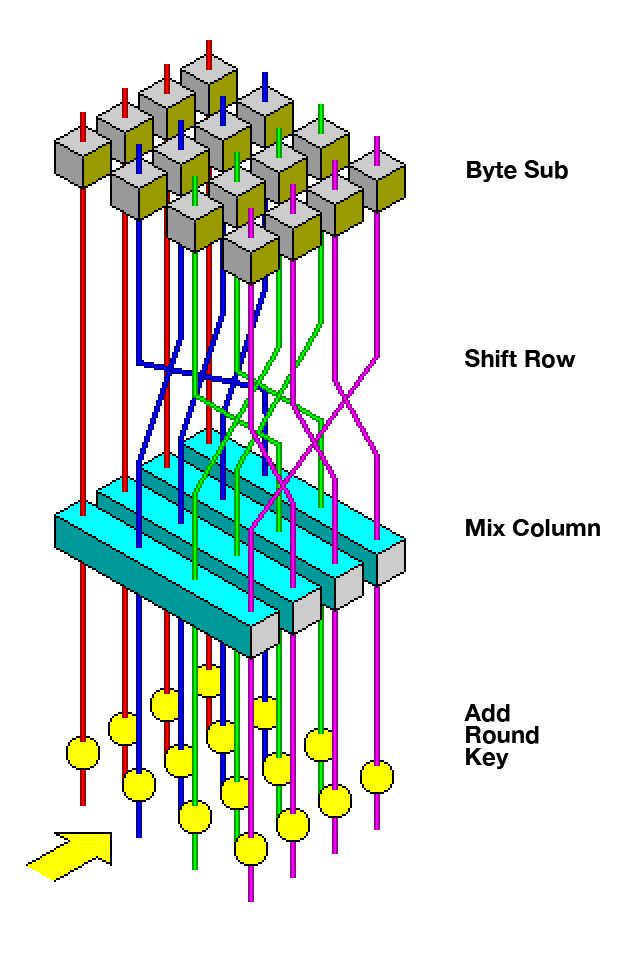
\includegraphics[width=0.45\columnwidth]{chapters/pictures/AES_(Rijndael)_Round_Function.png}
    \caption[Prikaz jedne runde AES šifrovanja]{Prikaz jedne runde AES šifrovanja. Preuzeto iz \cite{savard_aes_round}.}
    \label{fig:aes_runda}
\end{figure}

\subsection{Transformacije u rundi}
\label{subsec:aes_transformacije}

\subsubsection{SubBytes}

SubBytes zamenjuje svaki bajt matrice stanja vrednošću iz supstitucione tabele, S-boksa. Ta tabela nije proizvoljna, već je definisana kompozicijom dve operacije nad bajtom $b$:
\begin{enumerate}[itemsep=2pt]
    \item multiplikativna inverzija u polju $\mathrm{GF}(2^8)$ -- $b \mapsto b^{-1}$, uz dogovor $0 \mapsto 0$;
    \item afina transformacija nad bitovima rezultata:
    \begin{equation}
        b'_i = b_i \oplus b_{(i+4) \bmod 8} \oplus b_{(i+5) \bmod 8} \oplus b_{(i+6) \bmod 8} \oplus b_{(i+7) \bmod 8} \oplus c_i,
        \label{eq:sbox_afina}
    \end{equation}
    gde je $c = \{63\} = 01100011_2$.
\end{enumerate}
Inverzija u polju obezbeđuje visoku nelinearnost i otpornost na diferencijalnu i linearnu kriptoanalizu, dok afina transformacija otklanja fiksne tačke. U realizacijama se S-boks najčešće ostvaruje kao tabela od 256 vrednosti, memorijska ili kombinaciona, mada je moguće i direktno izračunavanje inverzije dekompozicijom polja, što je izbor koji neposredno utiče na površinu i kritičnu putanju hardvera. Transformacija deluje na svaki bajt nezavisno, pa se matrica stanja preslikava element po element, kako prikazuje slika \ref{fig:sbox_pristup}: gornja četiri bita bajta biraju vrstu, a donja četiri kolonu S-boksa. Na slici je istaknut bajt $\{53\}$, koji se preslikava u $\{ED\}$. Kompletna tabela S-boksa data je u dodatku \ref{app:aes_tabele}.

\begin{figure}[H]
\centering
\resizebox{\textwidth}{!}{
\begin{tikzpicture}
    \node (stanje) [inner sep=0pt] {%
    \begin{tabular}{|c|c|c|c|}
    \hline
    \rsz{1.3}{$s_{0,0}$} & \rsz{1.3}{$s_{0,1}$} & \rsz{1.3}{$s_{0,2}$} & \rsz{1.3}{$s_{0,3}$} \\ \hline
    \rsz{1.3}{$s_{1,0}$} & \cellcolor{green!30}\rsz{1.3}{$\{53\}$} & \rsz{1.3}{$s_{1,2}$} & \rsz{1.3}{$s_{1,3}$} \\ \hline
    \rsz{1.3}{$s_{2,0}$} & \rsz{1.3}{$s_{2,1}$} & \rsz{1.3}{$s_{2,2}$} & \rsz{1.3}{$s_{2,3}$} \\ \hline
    \rsz{1.3}{$s_{3,0}$} & \rsz{1.3}{$s_{3,1}$} & \rsz{1.3}{$s_{3,2}$} & \rsz{1.3}{$s_{3,3}$} \\ \hline
    \end{tabular}};
    \node (sbox) [blokkripto, right=1.6cm of stanje, minimum width=3.6cm, minimum height=3cm, align=center, font=\Large] {S-boks\\ $16 \times 16$\\ vrsta $\{5\}$, kolona $\{3\}$};
    \node (novo) [right=1.6cm of sbox, inner sep=0pt] {%
    \begin{tabular}{|c|c|c|c|}
    \hline
    \rsz{1.3}{$s'_{0,0}$} & \rsz{1.3}{$s'_{0,1}$} & \rsz{1.3}{$s'_{0,2}$} & \rsz{1.3}{$s'_{0,3}$} \\ \hline
    \rsz{1.3}{$s'_{1,0}$} & \cellcolor{purple!30}\rsz{1.3}{$\{ED\}$} & \rsz{1.3}{$s'_{1,2}$} & \rsz{1.3}{$s'_{1,3}$} \\ \hline
    \rsz{1.3}{$s'_{2,0}$} & \rsz{1.3}{$s'_{2,1}$} & \rsz{1.3}{$s'_{2,2}$} & \rsz{1.3}{$s'_{2,3}$} \\ \hline
    \rsz{1.3}{$s'_{3,0}$} & \rsz{1.3}{$s'_{3,1}$} & \rsz{1.3}{$s'_{3,2}$} & \rsz{1.3}{$s'_{3,3}$} \\ \hline
    \end{tabular}};
    \draw [strelica] (stanje) -- (sbox);
    \draw [strelica] (sbox) -- (novo);
\end{tikzpicture}
}
\caption{SubBytes transformacija na primeru bajta $\{53\} \mapsto \{ED\}$}
\label{fig:sbox_pristup}
\end{figure}

\subsubsection{ShiftRows}

ShiftRows ciklično pomera vrste matrice stanja ulevo. Vrsta $r$ pomera se za $r$ mesta, dakle nulta vrsta ostaje nepromenjena. Transformacija je prikazana na slici \ref{fig:shiftrows}. Kolone polazne matrice označene su bojama, pa se u rezultatu jasno vidi za koliko je mesta svaka vrsta pomerena.

\begin{figure}[H]
\centering
\resizebox{0.80\textwidth}{!}{
{\kvsetup
\begin{tabular}{c c c}
    \begin{tabular}[c]{|c|c|c|c|}
    \hline
    \cellcolor{green!30}\kv{$s_{0,0}$} & \cellcolor{cyan!30}\kv{$s_{0,1}$} & \cellcolor{yellow!30}\kv{$s_{0,2}$} & \cellcolor{purple!30}\kv{$s_{0,3}$} \\ \hline
    \cellcolor{green!30}\kv{$s_{1,0}$} & \cellcolor{cyan!30}\kv{$s_{1,1}$} & \cellcolor{yellow!30}\kv{$s_{1,2}$} & \cellcolor{purple!30}\kv{$s_{1,3}$} \\ \hline
    \cellcolor{green!30}\kv{$s_{2,0}$} & \cellcolor{cyan!30}\kv{$s_{2,1}$} & \cellcolor{yellow!30}\kv{$s_{2,2}$} & \cellcolor{purple!30}\kv{$s_{2,3}$} \\ \hline
    \cellcolor{green!30}\kv{$s_{3,0}$} & \cellcolor{cyan!30}\kv{$s_{3,1}$} & \cellcolor{yellow!30}\kv{$s_{3,2}$} & \cellcolor{purple!30}\kv{$s_{3,3}$} \\ \hline
    \end{tabular}
    &
    {\Huge $\longrightarrow$}
    &
    \begin{tabular}[c]{|c|c|c|c|}
    \hline
    \cellcolor{green!30}\kv{$s_{0,0}$} & \cellcolor{cyan!30}\kv{$s_{0,1}$} & \cellcolor{yellow!30}\kv{$s_{0,2}$} & \cellcolor{purple!30}\kv{$s_{0,3}$} \\ \hline
    \cellcolor{cyan!30}\kv{$s_{1,1}$} & \cellcolor{yellow!30}\kv{$s_{1,2}$} & \cellcolor{purple!30}\kv{$s_{1,3}$} & \cellcolor{green!30}\kv{$s_{1,0}$} \\ \hline
    \cellcolor{yellow!30}\kv{$s_{2,2}$} & \cellcolor{purple!30}\kv{$s_{2,3}$} & \cellcolor{green!30}\kv{$s_{2,0}$} & \cellcolor{cyan!30}\kv{$s_{2,1}$} \\ \hline
    \cellcolor{purple!30}\kv{$s_{3,3}$} & \cellcolor{green!30}\kv{$s_{3,0}$} & \cellcolor{cyan!30}\kv{$s_{3,1}$} & \cellcolor{yellow!30}\kv{$s_{3,2}$} \\ \hline
    \end{tabular}
\end{tabular}
}}
\caption{ShiftRows transformacija}
\label{fig:shiftrows}
\end{figure}

U hardveru je ShiftRows besplatna operacija, jer se svodi na preusmeravanje veza, bez logičkih elemenata i bez takta latencije.

\subsubsection{MixColumns}

MixColumns transformiše svaku kolonu matrice stanja množenjem fiksnom matricom nad $\mathrm{GF}(2^8)$:
\begin{equation}
\begin{bmatrix} s'_{0,c} \\ s'_{1,c} \\ s'_{2,c} \\ s'_{3,c} \end{bmatrix}
=
\begin{bmatrix}
\{02\} & \{03\} & \{01\} & \{01\} \\
\{01\} & \{02\} & \{03\} & \{01\} \\
\{01\} & \{01\} & \{02\} & \{03\} \\
\{03\} & \{01\} & \{01\} & \{02\}
\end{bmatrix}
\begin{bmatrix} s_{0,c} \\ s_{1,c} \\ s_{2,c} \\ s_{3,c} \end{bmatrix},
\qquad c = 0, \ldots, 3,
\label{eq:mixcolumns}
\end{equation}
gde vitičaste zagrade označavaju bajt u heksadecimalnom zapisu, tumačen kao element polja.
\smallbreak
Koeficijenti matrice nisu izabrani proizvoljno, nego tako da istovremeno ispune dva zahteva. Prvi je da difuzija bude najbolja moguća. Matrica je MDS (engl. \textit{Maximum Distance Separable}), pojam preuzet iz teorije kodova, koji ovde znači da je njena razgranatost (engl. \textit{branch number}) jednaka 5, pa zbir broja izmenjenih bajtova na ulazu i na izlazu ne može biti manji od 5. Praktična posledica je da promena makar jednog bajta u ulaznoj koloni menja sva četiri bajta izlazne kolone, što je najviše što se matricom $4 \times 4$ može postići \cite{daemen_rijndael}.
\smallbreak
Drugi zahtev je da množenja budu jeftina. Transformacija koristi samo koeficijente $\{01\}$, $\{02\}$ i $\{03\}$, a sva tri se svode na množenje sa $\{02\}$, koje u polju odgovara množenju polinoma sa $x$. Pošto bit $i$ bajta predstavlja koeficijent uz $x^i$, to je prosto pomeranje bajta ulevo. Ako pritom najstariji bit ispadne iz bajta, javlja se član $x^8$, pa se rezultat redukuje po modulu $m(x)$, odnosno sabira sa $\{1B\}$:
\begin{equation}
    \{02\} \cdot a =
    \begin{cases}
        a \ll 1, & a_7 = 0,\\[2pt]
        (a \ll 1) \oplus \{1B\}, & a_7 = 1.
    \end{cases}
    \label{eq:mul02}
\end{equation}
Množenje sa $\{03\}$ ne traži ništa novo, jer je $\{03\} \cdot a = \{02\} \cdot a \oplus a$. Cela MixColumns transformacija time se u hardveru svodi na pomeranja, uslovno sabiranje sa konstantom i XOR operacije, bez ijednog množača i bez tabele u memoriji.

\begin{example}
Kod množenja bajta $\{57\}$ sa $\{02\}$ najstariji bit od $01010111_2$ je nula, pa je rezultat samo pomeranje ulevo, $\{57\} \cdot \{02\} = 10101110_2 = \{AE\}$. Kod množenja $\{AE\}$ sa $\{02\}$ najstariji bit od $10101110_2$ je jedinica, pa se posle pomeranja ($01011100_2$) dodaje $\{1B\}$, dakle $\{AE\} \cdot \{02\} = 01011100_2 \oplus 00011011_2 = 01000111_2 = \{47\}$.
\end{example}

Slika \ref{fig:mixcolumns_sema} prikazuje delovanje transformacije. Svaka kolona nezavisno prolazi kroz blok koji izvršava množenje matricom iz izraza (\ref{eq:mixcolumns}), pa se u hardveru MixColumns prirodno realizuje sa četiri identična modula koji rade paralelno.

\begin{figure}[H]
\centering
\resizebox{\textwidth}{!}{
\begin{tikzpicture}
    \node (stanje) [inner sep=0pt] {%
    \begin{tabular}{|c|c|c|c|}
    \hline
    \rsz{1.3}{$s_{0,0}$} & \cellcolor{green!30}\rsz{1.3}{$s_{0,1}$} & \rsz{1.3}{$s_{0,2}$} & \rsz{1.3}{$s_{0,3}$} \\ \hline
    \rsz{1.3}{$s_{1,0}$} & \cellcolor{green!30}\rsz{1.3}{$s_{1,1}$} & \rsz{1.3}{$s_{1,2}$} & \rsz{1.3}{$s_{1,3}$} \\ \hline
    \rsz{1.3}{$s_{2,0}$} & \cellcolor{green!30}\rsz{1.3}{$s_{2,1}$} & \rsz{1.3}{$s_{2,2}$} & \rsz{1.3}{$s_{2,3}$} \\ \hline
    \rsz{1.3}{$s_{3,0}$} & \cellcolor{green!30}\rsz{1.3}{$s_{3,1}$} & \rsz{1.3}{$s_{3,2}$} & \rsz{1.3}{$s_{3,3}$} \\ \hline
    \end{tabular}};
    \node (m) [blokkripto, right=1.6cm of stanje, minimum width=3.6cm, minimum height=3cm, align=center, font=\Large] {množenje\\ matricom\\ iz (\ref{eq:mixcolumns})};
    \node (novo) [right=1.6cm of m, inner sep=0pt] {%
    \begin{tabular}{|c|c|c|c|}
    \hline
    \rsz{1.3}{$s_{0,0}$} & \cellcolor{purple!30}\rsz{1.3}{$s'_{0,1}$} & \rsz{1.3}{$s_{0,2}$} & \rsz{1.3}{$s_{0,3}$} \\ \hline
    \rsz{1.3}{$s_{1,0}$} & \cellcolor{purple!30}\rsz{1.3}{$s'_{1,1}$} & \rsz{1.3}{$s_{1,2}$} & \rsz{1.3}{$s_{1,3}$} \\ \hline
    \rsz{1.3}{$s_{2,0}$} & \cellcolor{purple!30}\rsz{1.3}{$s'_{2,1}$} & \rsz{1.3}{$s_{2,2}$} & \rsz{1.3}{$s_{2,3}$} \\ \hline
    \rsz{1.3}{$s_{3,0}$} & \cellcolor{purple!30}\rsz{1.3}{$s'_{3,1}$} & \rsz{1.3}{$s_{3,2}$} & \rsz{1.3}{$s_{3,3}$} \\ \hline
    \end{tabular}};
    \draw [strelica] (stanje) -- (m);
    \draw [strelica] (m) -- (novo);
\end{tikzpicture}
}
\caption{MixColumns transformacija nad jednom kolonom matrice stanja}
\label{fig:mixcolumns_sema}
\end{figure}

\subsubsection{AddRoundKey}

AddRoundKey sabira matricu stanja sa ključem tekuće runde operacijom XOR:
\begin{equation}
    s'_{r,c} = s_{r,c} \oplus k_{r,c}.
\end{equation}
Operacija je involutivna, jer ponovna primena istog ključa poništava njeno dejstvo, pa je pri dešifrovanju identična kao pri šifrovanju. Šematski prikaz dat je na slici \ref{fig:addroundkey_sema}.

\begin{figure}[H]
\centering
\begin{tikzpicture}
    \node (stanje) [blokdata, minimum width=2.8cm] {matrica stanja $s$};
    \node (xor) [circle, draw=black, thick, right=1.6cm of stanje, inner sep=2pt] {$\oplus$};
    \node (kljuc) [blokkripto, above=1cm of xor, minimum width=2.8cm] {ključ runde $k$};
    \node (novo) [blokrezultat, right=1.6cm of xor, minimum width=2.8cm] {novo stanje $s'$};
    \draw [strelica] (stanje) -- (xor);
    \draw [strelica] (kljuc) -- (xor);
    \draw [strelica] (xor) -- (novo);
\end{tikzpicture}
\caption{AddRoundKey transformacija}
\label{fig:addroundkey_sema}
\end{figure}

\subsection{Fuzija runde: T-tabele}
\label{subsec:aes_ttabele}

Cela runda, osim poslednje, može se stopiti u jednu tabelarnu operaciju. Ova tehnika, data već u izvornoj specifikaciji Rijndael algoritma \cite{daemen_rijndael}, prvobitno je smišljena za softverske realizacije na 32-bitnim procesorima, ali je jednako primenljiva u hardveru, gde je i korišćena u realizaciji opisanoj u poglavlju \ref{ch:hardver}.
\smallbreak
Posmatrajmo jednu kolonu izlaza runde. Kombinovanjem pomeranja vrsta sa slike \ref{fig:shiftrows} i množenja iz izraza (\ref{eq:mixcolumns}), kolona $c$ posle SubBytes, ShiftRows i MixColumns iznosi:
\begin{equation}
\begin{bmatrix} s'_{0,c} \\ s'_{1,c} \\ s'_{2,c} \\ s'_{3,c} \end{bmatrix}
=
\begin{bmatrix}
\{02\} & \{03\} & \{01\} & \{01\} \\
\{01\} & \{02\} & \{03\} & \{01\} \\
\{01\} & \{01\} & \{02\} & \{03\} \\
\{03\} & \{01\} & \{01\} & \{02\}
\end{bmatrix}
\begin{bmatrix} S[s_{0,c}] \\ S[s_{1,c+1}] \\ S[s_{2,c+2}] \\ S[s_{3,c+3}] \end{bmatrix},
\label{eq:runda_kolona}
\end{equation}
gde $S[\,\cdot\,]$ označava S-boks, a pomereni indeksi vrsta ($c+1$, $c+2$, $c+3$, po modulu 4) potiču od ShiftRows transformacije. Pošto je matrica konstantna, proizvod se može rastaviti na četiri sabirka, od kojih svaki zavisi od tačno jednog ulaznog bajta:
\begin{equation}
    \begin{bmatrix} s'_{0,c} \\ s'_{1,c} \\ s'_{2,c} \\ s'_{3,c} \end{bmatrix}
    = T_0\big[s_{0,c}\big] \oplus T_1\big[s_{1,c+1}\big] \oplus T_2\big[s_{2,c+2}\big] \oplus T_3\big[s_{3,c+3}\big],
    \label{eq:ttabela_kolona}
\end{equation}
gde su $T_0$ do $T_3$ tabele sa po 256 unosa od 32 bita, definisane kao:
\begin{align}
T_0[x] &= \begin{bmatrix} \{02\}\cdot S[x] \\ S[x] \\ S[x] \\ \{03\}\cdot S[x] \end{bmatrix}\!, &
T_1[x] &= \begin{bmatrix} \{03\}\cdot S[x] \\ \{02\}\cdot S[x] \\ S[x] \\ S[x] \end{bmatrix}\!, \nonumber\\[1.5ex]
T_2[x] &= \begin{bmatrix} S[x] \\ \{03\}\cdot S[x] \\ \{02\}\cdot S[x] \\ S[x] \end{bmatrix}\!, &
T_3[x] &= \begin{bmatrix} S[x] \\ S[x] \\ \{03\}\cdot S[x] \\ \{02\}\cdot S[x] \end{bmatrix}\!.
\label{eq:ttabele_def}
\end{align}
Dodavanjem ključa runde dobija se kompletna runda kao XOR pet 32-bitnih vrednosti:
\begin{equation}
    \text{kolona } c = T_0\big[s_{0,c}\big] \oplus T_1\big[s_{1,c+1}\big] \oplus T_2\big[s_{2,c+2}\big] \oplus T_3\big[s_{3,c+3}\big] \oplus K_c.
    \label{eq:ttabela_runda}
\end{equation}
Postupak je prikazan na slici \ref{fig:ttabele}.

\begin{figure}[H]
\centering
\resizebox{0.95\textwidth}{!}{
\begin{tikzpicture}
    \node (b0) [blokdata, minimum width=1.7cm] at (0,2.4) {$s_{0,c}$};
    \node (b1) [blokdata, minimum width=1.7cm] at (0,1.2) {$s_{1,c+1}$};
    \node (b2) [blokdata, minimum width=1.7cm] at (0,0) {$s_{2,c+2}$};
    \node (b3) [blokdata, minimum width=1.7cm] at (0,-1.2) {$s_{3,c+3}$};
    \node (t0) [blokkripto, minimum width=1.5cm] at (3.2,2.4) {$T_0$};
    \node (t1) [blokkripto, minimum width=1.5cm] at (3.2,1.2) {$T_1$};
    \node (t2) [blokkripto, minimum width=1.5cm] at (3.2,0) {$T_2$};
    \node (t3) [blokkripto, minimum width=1.5cm] at (3.2,-1.2) {$T_3$};
    \node (k) [blokdata, minimum width=1.7cm] at (3.2,-2.4) {$K_c$};
    \node (xor) [circle, draw=black, thick, inner sep=3pt] at (6.4,0.6) {$\oplus$};
    \node (out) [blokrezultat, minimum width=2.6cm] at (9.4,0.6) {kolona $c$};
    \foreach \i in {0,1,2,3} { \draw [strelica] (b\i) -- (t\i); }
    \foreach \i in {0,1,2,3} { \draw [strelica] (t\i) -- (xor); }
    \draw [strelica] (k) -- (xor);
    \draw [strelica] (xor) -- node[above, font=\small] {32 bita} (out);
    \node [font=\small, align=center] at (3.2,-3.5) {ShiftRows je sadržan\\ u izboru indeksa};
\end{tikzpicture}
}
\caption{Fuzija runde T-tabelama}
\label{fig:ttabele}
\end{figure}

Tri svojstva čine ovu transformaciju značajnom:
\begin{itemize}[itemsep=2pt]
    \item \textit{ShiftRows nestaje.} Ne izvršava se kao operacija, nego određuje samo koja četiri bajta stanja ulaze u koju kolonu. Ovaj dobitak pripada pre svega softveru. Na procesoru koji radi nad 32-bitnim rečima ShiftRows bi se izvodio nizom pomeranja i maskiranja pojedinačnih bajtova, dok je u hardveru i bez T-tabela bio puko preusmeravanje veza.
    \item \textit{Tabele su međusobno rotacije.} Iz definicije (\ref{eq:ttabele_def}) neposredno sledi da je $T_i[x]$ jednako $T_0[x]$ ciklično rotiranom za $i$ bajtova, pa je dovoljno čuvati samo $T_0$. Ostale tri su preuređenje bajtova, dakle besplatne.
    \item \textit{Cena je memorija umesto računa.} Jedna tabela zauzima $256 \times 32$ bita, odnosno 1 KB. Kolona se svodi na četiri čitanja i XOR umesto na lanac supstitucije i množenja u polju, a cela runda na šesnaest čitanja.
\end{itemize}
Poslednja runda nema MixColumns, pa se u njoj fuzija ne može primeniti. Ona se uvek realizuje neposredno. Hardverske posledice ovog izbora, uključujući pitanje koliko memorijskih blokova zaista košta, razmotrene su u odeljku \ref{subsec:hw_aes_round_style}.

\subsection{Ekspanzija ključa}
\label{subsec:aes_ekspanzija}

Za početnu operaciju i svaku od $N_r$ rundi potreban je poseban 128-bitni ključ runde, ukupno $N_b(N_r+1)$ kolona od po 32 bita. Za AES-256 to je 60 kolona, odnosno 15 ključeva rundi.
\smallbreak
Prošireni ključ se posmatra kao niz kolona $W_0, W_1, W_2, \ldots$, gde je svaka kolona reč od 32 bita, dakle četiri bajta. Pojedinačni bajt označava se sa $W_{i,j}$, pri čemu je $i \in \{0,1,2,3\}$ redni broj bajta unutar kolone, a $j$ redni broj same kolone. Ključ runde $r$ čine četiri uzastopne kolone, $W_{4r}$ do $W_{4r+3}$, tako da prvih $N_k$ kolona ne daje nužno ceo ključ prve runde. Kod AES-256 ulazni ključ od osam kolona daje ključ runde 0 i ključ runde 1.
\smallbreak
Kolone generiše ekspander ključa rekurzijom. Prvih $N_k$ kolona je sam ulazni ključ, a za $j \geq N_k$:
\begin{equation}
\small
W_j =
\begin{cases}
W_{j-N_k} \oplus \mathrm{SubWord}\big(\mathrm{RotWord}(W_{j-1})\big) \oplus \mathrm{Rcon}_{j/N_k}, & j \bmod N_k = 0,\\[4pt]
W_{j-N_k} \oplus \mathrm{SubWord}(W_{j-1}), & N_k > 6 \;\wedge\; j \bmod N_k = 4,\\[4pt]
W_{j-N_k} \oplus W_{j-1}, & \text{inače},
\end{cases}
\label{eq:key_expansion}
\end{equation}
Ovde $\mathrm{RotWord}$ ciklično rotira kolonu za jedan bajt naviše, a $\mathrm{SubWord}$ primenjuje S-boks na svaki od četiri bajta kolone.
\smallbreak
Konstanta runde $\mathrm{Rcon}_i$ je kolona kojoj su tri donja bajta nule, a gornji bajt je $(i{-}1)$-ti stepen elementa $\{02\}$ u polju $\mathrm{GF}(2^8)$:
\begin{equation}
    \mathrm{Rcon}_i = \big(\{02\}^{\,i-1},\; \{00\},\; \{00\},\; \{00\}\big).
    \label{eq:rcon}
\end{equation}
Pošto je množenje sa $\{02\}$ upravo pomeranje ulevo iz izraza (\ref{eq:mul02}), niz konstanti počinje kao $\{01\}, \{02\}, \{04\}, \{08\}, \{10\}, \{20\}, \{40\}, \{80\}$, a zatim, kada pomeranje izbaci najstariji bit, sledi redukcija: $\{80\} \cdot \{02\} = \{1B\}$, pa $\{36\}$ i tako dalje. Uloga ovih konstanti je da razbiju pravilnosti ekspanzije. Bez njih bi se svaka grupa od $N_k$ kolona računala potpuno istim pravilom, a ekspanzija bi uz to bila invarijantna na rotaciju bajtova unutar kolone. $\mathrm{Rcon}$ je jedina veličina vezana i za konkretnu grupu i za konkretan bajt, pa obe pravilnosti nestaju. Detaljnije obrazloženje dato je u \cite{daemen_rijndael}, a sve vrednosti konstanti u dodatku \ref{app:rcon}.
\smallbreak
Srednja grana rekurzije postoji samo kod AES-256 ($N_k = 8$) i unosi dodatnu nelinearnost u sredinu svake grupe od osam kolona. Struktura rekurzije prikazana je na slici \ref{fig:ekspanzija_256}. Nova kolona se uvek dobija sabiranjem kolone udaljene $N_k$ mesta i, po potrebi transformisane, prethodne kolone, pri čemu $S[\,\cdot\,]$ označava primenu S-boksa na bajt.

\begin{figure}[H]
\centering
\resizebox{0.95\textwidth}{!}{
\begin{tabular}{c}
% slucaj j = 0 (mod 8)
\begin{tabular}{c c c c c c c c}
    \raisebox{-7ex}{\Large $j \equiv 0 \!\!\pmod 8$:} &
    \begin{tabular}{|c|}
    \multicolumn{1}{c}{\rsz[1.8cm]{1.2}{$W_{j-8}$}} \\
    \hline
    \cellcolor{green!30}\rsz[1.8cm]{1.3}{$W_{0,j-8}$} \\ \hline
    \cellcolor{green!30}\rsz[1.8cm]{1.3}{$W_{1,j-8}$} \\ \hline
    \cellcolor{green!30}\rsz[1.8cm]{1.3}{$W_{2,j-8}$} \\ \hline
    \cellcolor{green!30}\rsz[1.8cm]{1.3}{$W_{3,j-8}$} \\ \hline
    \end{tabular}
    & \raisebox{-7ex}{\Huge $\oplus$} &
    \begin{tabular}{|c|}
    \multicolumn{1}{c}{\rsz[3cm]{1.2}{$\mathrm{rot}\big(S[W_{j-1}]\big)$}} \\
    \hline
    \cellcolor{yellow!30}\rsz[2.6cm]{1.3}{$S[W_{1,j-1}]$} \\ \hline
    \cellcolor{yellow!30}\rsz[2.6cm]{1.3}{$S[W_{2,j-1}]$} \\ \hline
    \cellcolor{yellow!30}\rsz[2.6cm]{1.3}{$S[W_{3,j-1}]$} \\ \hline
    \cellcolor{yellow!30}\rsz[2.6cm]{1.3}{$S[W_{0,j-1}]$} \\ \hline
    \end{tabular}
    & \raisebox{-7ex}{\Huge $\oplus$} &
    \begin{tabular}{|c|}
    \multicolumn{1}{c}{\rsz[2cm]{1.2}{$\mathrm{Rcon}_{j/8}$}} \\
    \hline
    \cellcolor{gray!30}\rsz[2.2cm]{1.3}{$\{02\}^{j/8-1}$} \\ \hline
    \cellcolor{gray!30}\rsz[1.8cm]{1.3}{$\{00\}$} \\ \hline
    \cellcolor{gray!30}\rsz[1.8cm]{1.3}{$\{00\}$} \\ \hline
    \cellcolor{gray!30}\rsz[1.8cm]{1.3}{$\{00\}$} \\ \hline
    \end{tabular}
    & \raisebox{-7ex}{\Huge $=$} &
    \begin{tabular}{|c|}
    \multicolumn{1}{c}{\rsz[1.6cm]{1.2}{$W_{j}$}} \\
    \hline
    \cellcolor{purple!30}\rsz[1.6cm]{1.3}{$W_{0,j}$} \\ \hline
    \cellcolor{purple!30}\rsz[1.6cm]{1.3}{$W_{1,j}$} \\ \hline
    \cellcolor{purple!30}\rsz[1.6cm]{1.3}{$W_{2,j}$} \\ \hline
    \cellcolor{purple!30}\rsz[1.6cm]{1.3}{$W_{3,j}$} \\ \hline
    \end{tabular}
\end{tabular}
\\[4ex]
% slucaj j = 4 (mod 8)
\begin{tabular}{c c c c c c}
    \raisebox{-7ex}{\Large $j \equiv 4 \!\!\pmod 8$:} &
    \begin{tabular}{|c|}
    \multicolumn{1}{c}{\rsz[1.8cm]{1.2}{$W_{j-8}$}} \\
    \hline
    \cellcolor{green!30}\rsz[1.8cm]{1.3}{$W_{0,j-8}$} \\ \hline
    \cellcolor{green!30}\rsz[1.8cm]{1.3}{$W_{1,j-8}$} \\ \hline
    \cellcolor{green!30}\rsz[1.8cm]{1.3}{$W_{2,j-8}$} \\ \hline
    \cellcolor{green!30}\rsz[1.8cm]{1.3}{$W_{3,j-8}$} \\ \hline
    \end{tabular}
    & \raisebox{-7ex}{\Huge $\oplus$} &
    \begin{tabular}{|c|}
    \multicolumn{1}{c}{\rsz[2.4cm]{1.2}{$S[W_{j-1}]$}} \\
    \hline
    \cellcolor{yellow!30}\rsz[2.6cm]{1.3}{$S[W_{0,j-1}]$} \\ \hline
    \cellcolor{yellow!30}\rsz[2.6cm]{1.3}{$S[W_{1,j-1}]$} \\ \hline
    \cellcolor{yellow!30}\rsz[2.6cm]{1.3}{$S[W_{2,j-1}]$} \\ \hline
    \cellcolor{yellow!30}\rsz[2.6cm]{1.3}{$S[W_{3,j-1}]$} \\ \hline
    \end{tabular}
    & \raisebox{-7ex}{\Huge $=$} &
    \begin{tabular}{|c|}
    \multicolumn{1}{c}{\rsz[1.6cm]{1.2}{$W_{j}$}} \\
    \hline
    \cellcolor{purple!30}\rsz[1.6cm]{1.3}{$W_{0,j}$} \\ \hline
    \cellcolor{purple!30}\rsz[1.6cm]{1.3}{$W_{1,j}$} \\ \hline
    \cellcolor{purple!30}\rsz[1.6cm]{1.3}{$W_{2,j}$} \\ \hline
    \cellcolor{purple!30}\rsz[1.6cm]{1.3}{$W_{3,j}$} \\ \hline
    \end{tabular}
\end{tabular}
\\[4ex]
% ostali slucajevi
\begin{tabular}{c c c c c c}
    \raisebox{-7ex}{\Large inače:} &
    \begin{tabular}{|c|}
    \multicolumn{1}{c}{\rsz[1.8cm]{1.2}{$W_{j-8}$}} \\
    \hline
    \cellcolor{green!30}\rsz[1.8cm]{1.3}{$W_{0,j-8}$} \\ \hline
    \cellcolor{green!30}\rsz[1.8cm]{1.3}{$W_{1,j-8}$} \\ \hline
    \cellcolor{green!30}\rsz[1.8cm]{1.3}{$W_{2,j-8}$} \\ \hline
    \cellcolor{green!30}\rsz[1.8cm]{1.3}{$W_{3,j-8}$} \\ \hline
    \end{tabular}
    & \raisebox{-7ex}{\Huge $\oplus$} &
    \begin{tabular}{|c|}
    \multicolumn{1}{c}{\rsz[1.8cm]{1.2}{$W_{j-1}$}} \\
    \hline
    \cellcolor{green!30}\rsz[1.8cm]{1.3}{$W_{0,j-1}$} \\ \hline
    \cellcolor{green!30}\rsz[1.8cm]{1.3}{$W_{1,j-1}$} \\ \hline
    \cellcolor{green!30}\rsz[1.8cm]{1.3}{$W_{2,j-1}$} \\ \hline
    \cellcolor{green!30}\rsz[1.8cm]{1.3}{$W_{3,j-1}$} \\ \hline
    \end{tabular}
    & \raisebox{-7ex}{\Huge $=$} &
    \begin{tabular}{|c|}
    \multicolumn{1}{c}{\rsz[1.6cm]{1.2}{$W_{j}$}} \\
    \hline
    \cellcolor{purple!30}\rsz[1.6cm]{1.3}{$W_{0,j}$} \\ \hline
    \cellcolor{purple!30}\rsz[1.6cm]{1.3}{$W_{1,j}$} \\ \hline
    \cellcolor{purple!30}\rsz[1.6cm]{1.3}{$W_{2,j}$} \\ \hline
    \cellcolor{purple!30}\rsz[1.6cm]{1.3}{$W_{3,j}$} \\ \hline
    \end{tabular}
\end{tabular}
\end{tabular}
}
\caption{Ekspanzija ključa za AES-256: izračunavanje kolone $W_j$, $j \geq 8$, po slučajevima}
\label{fig:ekspanzija_256}
\end{figure}

\subsection{Dešifrovanje}
\label{subsec:aes_dekripcija}

Sve transformacije AES algoritma su invertibilne, pa standard \cite{fips197} uz šifrovanje definiše i inverznu šifru. Transformacije \mbox{InvSubBytes}, \mbox{InvShiftRows} i \mbox{InvMixColumns} primenjuju se obrnutim redosledom, sa ključevima rundi uzetim od poslednjeg ka prvom. Za ovaj rad je bitno da režimi CTR familije, kojoj pripada i GCM, blok šifru pozivaju isključivo u smeru šifrovanja, i pri šifrovanju i pri dešifrovanju, kako je pokazano u odeljku \ref{subsubsec:ctr_rezim}. Inverzna šifra zato u realizaciji nije ni potrebna.

\subsection{Režimi rada blok šifara}
\label{subsec:rezimi_rada_detaljno}

AES definiše transformaciju samo nad jednim blokom od 128 bitova. Način primene šifre na poruke proizvoljne dužine određuje režim rada. Izbor režima određuje i sigurnosna svojstva koja sistem pruža i strukturu hardvera koji ga realizuje. U nastavku su razmotrena tri karakteristična režima, redosledom koji vodi ka GCM-u.

\subsubsection{ECB režim}

ECB (engl. \textit{Electronic Codebook}) je najjednostavniji režim, u kome se svaki blok šifruje nezavisno istim ključem,
\begin{equation}
    \mathrm{CT}_i = E_K(\mathrm{PT}_i).
\end{equation}
Posledica je da identični blokovi otvorenog teksta daju identične blokove šifrata, pa statistička struktura poruke ostaje vidljiva u šifratu. Slika \ref{fig:modovi_pecat} ovo čini očiglednim. Na slici pečata šifrovanoj u ECB režimu pozadina se preslikava u identične vrednosti i kontura pečata se jasno nazire, dok se CBC i CTR šifrati ne razlikuju od šuma. Detaljna kritička analiza ECB režima data je u \cite{gavrilovic_diplomski}.

\begin{figure}[H]
    \centering
    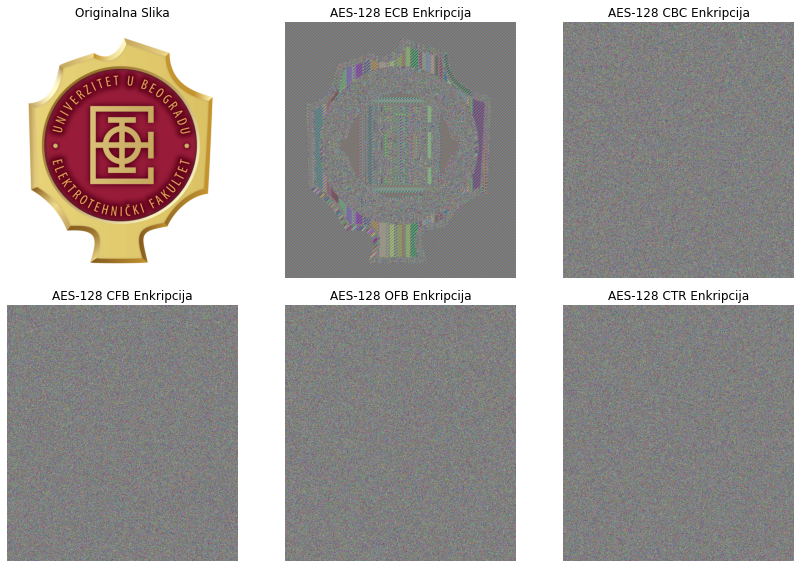
\includegraphics[width=0.9\columnwidth]{chapters/pictures/Modovi_rada_AES.png}
    \caption[AES-128 šifrovanje slike u različitim režimima rada]{AES-128 šifrovanje slike u različitim režimima rada. Preuzeto iz \cite{gavrilovic_diplomski}.}
    \label{fig:modovi_pecat}
\end{figure}

\subsubsection{CBC režim}

CBC (engl. \textit{Cipher Block Chaining}) otklanja slabost ECB režima ulančavanjem blokova, pri kome se svaki blok otvorenog teksta pre šifrovanja sabira sa prethodnim blokom šifrata,
\begin{equation}
    \mathrm{CT}_i = E_K(\mathrm{PT}_i \oplus \mathrm{CT}_{i-1}), \qquad \mathrm{CT}_0 = IV,
\end{equation}
gde je $IV$ nasumični inicijalizacioni vektor. Identični blokovi otvorenog teksta sada daju različite šifrate, ali se cena plaća upravo u onome što je za hardver najvažnije, u propusnosti. Šifrovanje bloka $i$ ne može početi pre nego što se završi blok $i-1$. Povratna sprega onemogućava protočnu obradu, pa AES jezgro sa latencijom od $L$ taktova postiže tek jedan blok na svakih $L$ taktova, ma koliko resursa bilo na raspolaganju. Pored toga, CBC zahteva dopunu poruke do umnoška bloka i koristi i smer dešifrovanja.

\subsubsection{CTR režim}
\label{subsubsec:ctr_rezim}

CTR (engl. \textit{Counter}) režim ide drugim putem. Umesto ulančavanja podataka šifruje se niz vrednosti brojača, a dobijeni pseudoslučajni niz sabira sa otvorenim tekstom,
\begin{equation}
    \mathrm{CT}_i = \mathrm{PT}_i \oplus E_K(IV \,\|\, i),
    \label{eq:ctr_generic}
\end{equation}
čime se blok šifra efektivno pretvara u protočnu šifru, a šema režima prikazana je na slici \ref{fig:ctr_sema}.

\begin{figure}[H]
\centering
\resizebox{0.8\textwidth}{!}{
\begin{tikzpicture}
    \node (cb1) [blokdata, minimum width=2.4cm] {$IV \,\|\, 1$};
    \node (ek1) [blokkripto, below=0.7cm of cb1, minimum width=2.4cm] {$E_K$};
    \node (xor1) [circle, draw=black, thick, below=0.7cm of ek1, inner sep=2pt] {$\oplus$};
    \node (p1) [blokdata, left=1cm of xor1, minimum width=1.4cm] {$\mathrm{PT}_1$};
    \node (c1) [blokrezultat, below=0.7cm of xor1, minimum width=1.4cm] {$\mathrm{CT}_1$};
    \draw [strelica] (cb1) -- (ek1);
    \draw [strelica] (ek1) -- (xor1);
    \draw [strelica] (p1) -- (xor1);
    \draw [strelica] (xor1) -- (c1);

    \node (cb2) [blokdata, right=2.4cm of cb1, minimum width=2.4cm] {$IV \,\|\, 2$};
    \node (ek2) [blokkripto, below=0.7cm of cb2, minimum width=2.4cm] {$E_K$};
    \node (xor2) [circle, draw=black, thick, below=0.7cm of ek2, inner sep=2pt] {$\oplus$};
    \node (p2) [blokdata, left=1cm of xor2, minimum width=1.4cm] {$\mathrm{PT}_2$};
    \node (c2) [blokrezultat, below=0.7cm of xor2, minimum width=1.4cm] {$\mathrm{CT}_2$};
    \draw [strelica] (cb2) -- (ek2);
    \draw [strelica] (ek2) -- (xor2);
    \draw [strelica] (p2) -- (xor2);
    \draw [strelica] (xor2) -- (c2);

    \node (dots) [right=1.2cm of ek2] {\Huge $\cdots$};
\end{tikzpicture}
}
\caption{CTR režim rada: blokovi se obrađuju nezavisno i paralelno}
\label{fig:ctr_sema}
\end{figure}

Svojstva CTR režima čine ga idealnim polazištem za hardver visoke propusnosti. Blokovi su potpuno nezavisni, jer brojački blok ne zavisi od podataka, pa je moguća i savršena protočnost i paralelizam. Poruka ne zahteva dopunu, jer se od poslednjeg bloka pseudoslučajnog niza uzima tačno onoliko bitova koliko je potrebno. Uz to, dešifrovanje je identičan postupak. Primalac istim ključem i istim brojačkim blokovima proizvede isti pseudoslučajni niz i sabere ga sa šifratom, pa se blok šifra i pri dešifrovanju poziva samo u smeru šifrovanja, a inverzna šifra iz odeljka \ref{subsec:aes_dekripcija} nije potrebna. Kritičan zahtev je da se vrednost brojača nikada ne ponovi sa istim ključem.

\subsubsection{Od CTR do GCM}

CTR režim, međutim, ne pruža nikakvu zaštitu integriteta. Štaviše, izrazito je savitljiv (engl. \textit{malleable}). Pošto je $\mathrm{CT}_i = \mathrm{PT}_i \oplus ks_i$, ako Oskar promeni proizvoljan bit šifrata, promenio je tačno taj bit dešifrovanog teksta, predvidljivo i neprimetno. Šifrovana poruka se stoga u praksi mora štititi i kodom za autentifikaciju, a GCM je upravo standardizovan odgovor na tu potrebu, sa CTR režimom za poverljivost i GHASH funkcijom za integritet, uz obradu pridruženih podataka. Tabela \ref{tab:ctr_vs_gcm} sumira poređenje.

\begin{table}[H]
\caption{Poređenje CTR i GCM režima rada}
\centering
\resizebox{0.95\textwidth}{!}{
\begin{tabular}{|c|c|c|}
\hline
\rowcolor{gray!30}
Svojstvo & CTR & GCM \\
\hline
poverljivost & da & da \\
\hline
integritet i autentifikacija poruke & ne & da \\
\hline
pridruženi podaci (AAD) & ne & da \\
\hline
paralelna obrada blokova & da & \makecell{da za šifrovanje, a autentifikacija je serijska, jedno \\ množenje po bloku (odeljak \ref{subsubsec:ghash_paralelizacija})} \\
\hline
koristi samo smer šifrovanja & da & da \\
\hline
dodatni hardver & --- & množač u GF($2^{128}$) (GHASH) \\
\hline
\end{tabular}
}
\label{tab:ctr_vs_gcm}
\end{table}

\subsection{GCM režim rada}
\label{subsec:gcm_rezim}

GCM (engl. \textit{Galois/Counter Mode}) \cite{sp80038d, mcgrew_viega} je AEAD režim rada koji objedinjuje dva gradivna elementa: CTR režim šifrovanja, zadužen za poverljivost, i GHASH funkciju autentifikacije, zaduženu za integritet. Ulaz u GCM šifrovanje čine:
\begin{itemize}[itemsep=2pt]
    \item tajni ključ $K$ (u ovom radu 256-bitni),
    \item nonce vrednost $IV$, jedinstvena za svaku poruku šifrovanu istim ključem,
    \item otvoreni tekst $\mathrm{PT}$ (engl. \textit{plaintext}) proizvoljne dužine,
    \item pridruženi podaci $\mathrm{AAD}$, koji se ne šifruju, ali ulaze u autentifikaciju. Tipično su to zaglavlja mrežnih paketa, koja moraju ostati čitljiva usput, a ne smeju biti izmenjena.
\end{itemize}
Izlaz su šifrat $\mathrm{CT}$ (engl. \textit{ciphertext}), iste dužine kao $\mathrm{PT}$, i autentifikaciona oznaka $\mathrm{ICV}$ (engl. \textit{Integrity Check Value}).
\smallbreak
Postupak počinje izvođenjem dve vrednosti. Prva je heš potključ (engl. \textit{hash subkey}):
\begin{equation}
    H = E_K(0^{128}),
\end{equation}
dobijen šifrovanjem nultog bloka, koji parametrizuje GHASH funkciju, a druga je početni brojački blok $J_0$. Za preporučenu dužinu nonce vrednosti od 96 bitova formira se jednostavnim nadovezivanjem,
\begin{equation}
    J_0 = IV \,\|\, 0^{31} \,\|\, 1,
    \label{eq:j0}
\end{equation}
dok se za ostale dužine $IV$ izvodi GHASH funkcijom nad dopunjenim $IV$. Upravo zbog jednostavnosti izraza (\ref{eq:j0}) hardverske realizacije po pravilu fiksiraju dužinu nonce vrednosti na 96 bitova.

\subsubsection{CTR šifrovanje}

Otvoreni tekst deli se na $n = \lceil \mathrm{len}(\mathrm{PT})/128 \rceil$ blokova $\mathrm{PT}_1, \ldots, \mathrm{PT}_n$, pri čemu poslednji blok može biti nepotpun. \textit{Brojački blokovi} (engl. \textit{counter block}) $CB_i$ generišu se funkcijom $\mathrm{inc_{32}}$, koja inkrementira najnižih 32 bita bloka po modulu $2^{32}$, ne dirajući gornjih 96 bitova:
\begin{equation}
    CB_1 = \mathrm{inc_{32}}(J_0), \qquad CB_i = \mathrm{inc_{32}}(CB_{i-1}), \quad i = 2, \ldots, n.
\end{equation}
Svaki brojački blok se šifruje, a rezultat sabira operacijom XOR sa odgovarajućim blokom otvorenog teksta:
\begin{equation}
    \mathrm{CT}_i = \mathrm{PT}_i \oplus E_K(CB_i), \qquad i = 1, \ldots, n-1,
\end{equation}
dok se za poslednji, potencijalno nepotpun blok dužine $u$ bitova koristi samo najznačajnijih $u$ bitova šifrovanog brojača:
\begin{equation}
    \mathrm{CT}_n = \mathrm{PT}_n \oplus \mathrm{MSB}_u\big(E_K(CB_n)\big).
\end{equation}
Brojački niz počinje od $J_0$, ali šifrovanje podataka počinje tek od $CB_1$, jer sam $J_0$ nikada ne šifruje podatke, nego je njegov šifrat $E_K(J_0)$ rezervisan za masku autentifikacione oznake u izrazu (\ref{eq:gcm_tag}). Time nijedan blok pseudoslučajnog niza nije upotrebljen dvaput, jer se maska oznake ne poklapa ni sa jednim blokom koji štiti podatke. Grana za poverljivost je, dakle, običan CTR režim nad blokovima $CB_1, \ldots, CB_n$, pa za nju važe sva svojstva iz odeljka \ref{subsec:rezimi_rada_detaljno}, pre svega protočna obrada bez povratne sprege.

\subsubsection{GHASH funkcija}
\label{subsubsec:ghash}

Autentifikacija u GCM režimu zasniva se na funkciji GHASH, definisanoj nad poljem $\mathrm{GF}(2^{128})$ sa redukcionim polinomom:
\begin{equation}
    f(x) = x^{128} + x^7 + x^2 + x + 1.
    \label{eq:gcm_polinom}
\end{equation}
Blokovi poruke tumače se kao koeficijenti polinoma nad tim poljem, a sažetak je vrednost tog polinoma u tački $H$. Za niz 128-bitnih blokova $X_1, X_2, \ldots, X_m$ to znači:
\begin{equation}
    \mathrm{GHASH}_H(X) = X_1 \cdot H^m \oplus X_2 \cdot H^{m-1} \oplus \cdots \oplus X_m \cdot H.
    \label{eq:ghash_polinom}
\end{equation}
Pošto je $H$ tajan, Oskar ne zna u kojoj se tački polinom računa, pa ne može da nađe drugu poruku sa istom vrednošću. Konstrukcije ovog tipa u literaturi se zovu univerzalne heš funkcije (engl. \textit{universal hash function}). Za razliku od SHA-3, one nisu sigurne same po sebi, nego tek uz tajni parametar i jednokratnu masku.
\smallbreak
Izraz (\ref{eq:ghash_polinom}) se ne izračunava neposredno, jer bi tražio sve stepene $H^2, \ldots, H^m$, nego Hornerovom šemom, u kojoj se svaki blok sabere sa akumulatorom, a zbir pomnoži sa $H$:
\begin{equation}
    Y_0 = 0^{128}, \qquad Y_i = (Y_{i-1} \oplus X_i) \cdot H, \qquad \mathrm{GHASH}_H(X) = Y_m.
    \label{eq:ghash_horner}
\end{equation}
Time je po bloku potrebno jedno jedino množenje u polju, i to sa uvek istim činiocem $H$. Sekvencijalni tok izračunavanja prikazan je na slici \ref{fig:ghash_lanac}.
\smallbreak
Ostaje još jedan detalj zapisa. Standard \cite{sp80038d} bitove 128-bitnog bloka pridružuje stepenima ogledalski u odnosu na uobičajeni binarni zapis. Krajnji levi bit bloka je koeficijent uz $x^0$, a krajnji desni uz $x^{127}$. Na matematička svojstva polja to nema uticaja, a u hardveru se svodi na preuređenje veza na ulazu i izlazu množača, bez ijednog logičkog elementa. Jedini uslov je da ono bude dosledno sprovedeno.

\begin{figure}[H]
\centering
\resizebox{0.95\textwidth}{!}{
\begin{tikzpicture}
    \node (y0) [blokdata, minimum width=1.8cm] {$Y_0 = 0$};
    \node (xor1) [circle, draw=black, thick, right=0.9cm of y0, inner sep=2pt] {$\oplus$};
    \node (x1) [blokdata, above=0.7cm of xor1, minimum width=1.2cm] {$X_1$};
    \node (h1) [blokghash, right=0.9cm of xor1, minimum width=1.3cm] {$\cdot\, H$};
    \node (xor2) [circle, draw=black, thick, right=0.9cm of h1, inner sep=2pt] {$\oplus$};
    \node (x2) [blokdata, above=0.7cm of xor2, minimum width=1.2cm] {$X_2$};
    \node (h2) [blokghash, right=0.9cm of xor2, minimum width=1.3cm] {$\cdot\, H$};
    \node (xor3) [circle, draw=black, thick, right=0.9cm of h2, inner sep=2pt] {$\oplus$};
    \node (x3) [blokdata, above=0.7cm of xor3, minimum width=1.2cm] {$X_3$};
    \node (h3) [blokghash, right=0.9cm of xor3, minimum width=1.3cm] {$\cdot\, H$};
    \node (ym) [blokrezultat, right=0.9cm of h3, minimum width=1.4cm] {$Y_3$};
    \draw [strelica] (y0) -- (xor1);
    \draw [strelica] (x1) -- (xor1);
    \draw [strelica] (xor1) -- (h1);
    \draw [strelica] (h1) -- node[below] {\small $Y_1$} (xor2);
    \draw [strelica] (x2) -- (xor2);
    \draw [strelica] (xor2) -- (h2);
    \draw [strelica] (h2) -- node[below] {\small $Y_2$} (xor3);
    \draw [strelica] (x3) -- (xor3);
    \draw [strelica] (xor3) -- (h3);
    \draw [strelica] (h3) -- (ym);
\end{tikzpicture}
}
\caption{GHASH funkcija kao Hornerova šema}
\label{fig:ghash_lanac}
\end{figure} Ulazni niz GHASH funkcije formira se nadovezivanjem pridruženih podataka $\mathrm{AAD}$ i šifrata $\mathrm{CT}$, svakog dopunjenog nulama do umnoška 128 bitova, i završnog bloka koji sadrži 64-bitne zapise njihovih dužina:
\begin{equation}
    S = \mathrm{GHASH}_H\big(\mathrm{AAD} \,\|\, 0^{v} \,\|\, \mathrm{CT} \,\|\, 0^{w} \,\|\, \mathrm{len}_{64}(\mathrm{AAD}) \,\|\, \mathrm{len}_{64}(\mathrm{CT})\big).
    \label{eq:ghash_ulaz}
\end{equation}
gde su $v$ i $w$ najmanji brojevi nula koji dužine $\mathrm{AAD}$ i $\mathrm{CT}$ dovode do umnoška 128 bitova. Uključivanje dužina u poslednji blok sprečava napade produžavanjem i preraspodelom granice između $\mathrm{AAD}$ i $\mathrm{CT}$. Konačno, oznaka se dobija šifrovanjem vrednosti $S$ blokom $J_0$:
\begin{equation}
    \mathrm{ICV} = \mathrm{MSB}_t\big(E_K(J_0) \oplus S\big),
    \label{eq:gcm_tag}
\end{equation}
gde je $t$ dužina oznake (pun format je $t = 128$). Ovaj korak je i razlog zašto sama GHASH funkcija ne mora biti kriptografski sigurna. Vrednost $S$ nikada ne napušta jezgro nezaštićena, nego se sabira sa maskom $E_K(J_0)$, koja je za svaku poruku druga. Bez poznavanja ključa Oskar ne može izračunati tu masku, pa ni konstruisati ispravnu oznaku za izmenjenu poruku. Celokupan postupak GCM šifrovanja, sa CTR granom i GHASH granom kao odvojenim funkcionalnim celinama, prikazan je na slici \ref{fig:gcm_sema} na primeru poruke od dva bloka. Blok $L$ na slici je završni blok sa dužinama, $L = \mathrm{len}_{64}(\mathrm{AAD}) \,\|\, \mathrm{len}_{64}(\mathrm{CT})$, iz izraza (\ref{eq:ghash_ulaz}).

\begin{figure}[H]
\centering
\resizebox{0.95\textwidth}{!}{
\begin{tikzpicture}
    % CTR grana
    \node (iv) [blokdata, minimum width=2cm] {$IV$};
    \node (j0) [blokdata, right=1.4cm of iv, minimum width=2cm] {$J_0$};
    \node (cb1) [blokdata, right=2cm of j0, minimum width=2cm] {$CB_1$};
    \node (cb2) [blokdata, right=2cm of cb1, minimum width=2cm] {$CB_2$};
    \draw [strelica] (iv) -- node[above] {\small $\|\, 0^{31} 1$} (j0);
    \draw [strelica] (j0) -- node[above] {\small $\mathrm{inc_{32}}$} (cb1);
    \draw [strelica] (cb1) -- node[above] {\small $\mathrm{inc_{32}}$} (cb2);

    \node (ek0) [blokkripto, below=0.9cm of j0, minimum width=2cm] {$E_K$};
    \node (ek1) [blokkripto, below=0.9cm of cb1, minimum width=2cm] {$E_K$};
    \node (ek2) [blokkripto, below=0.9cm of cb2, minimum width=2cm] {$E_K$};
    \draw [strelica] (j0) -- (ek0);
    \draw [strelica] (cb1) -- (ek1);
    \draw [strelica] (cb2) -- (ek2);

    \node (xor1) [circle, draw=black, thick, below=0.9cm of ek1, inner sep=2pt] {$\oplus$};
    \node (xor2) [circle, draw=black, thick, below=0.9cm of ek2, inner sep=2pt] {$\oplus$};
    \node (p1) [blokdata, right=0.6cm of xor1, minimum width=1.1cm] {$\mathrm{PT}_1$};
    \node (p2) [blokdata, right=0.6cm of xor2, minimum width=1.1cm] {$\mathrm{PT}_2$};
    \draw [strelica] (ek1) -- (xor1);
    \draw [strelica] (ek2) -- (xor2);
    \draw [strelica] (p1) -- (xor1);
    \draw [strelica] (p2) -- (xor2);

    \node (c1) [blokrezultat, below=0.8cm of xor1, minimum width=1.4cm] {$\mathrm{CT}_1$};
    \node (c2) [blokrezultat, below=0.8cm of xor2, minimum width=1.4cm] {$\mathrm{CT}_2$};
    \draw [strelica] (xor1) -- (c1);
    \draw [strelica] (xor2) -- (c2);

    % GHASH grana
    \node (ghash) [blokghash, below=1.3cm of c1, xshift=2cm, minimum width=6.4cm, minimum height=1.1cm] {$\mathrm{GHASH}_H$};
    \node (aad) [blokdata, left=1.6cm of ghash, minimum width=1.1cm] {$\mathrm{AAD}$};
    \node (len) [blokdata, right=1.6cm of ghash, minimum width=1.1cm] {$L$};
    \draw [strelica] (c1) -- (ghash);
    \draw [strelica] (c2) -- (ghash);
    \draw [strelica] (aad) -- (ghash);
    \draw [strelica] (len) -- (ghash);

    \node (xort) [circle, draw=black, thick, below=0.9cm of ghash, inner sep=2pt] {$\oplus$};
    \draw [strelica] (ghash) -- node[right] {\small $S$} (xort);
    \draw [strelica] (ek0) |- node[below left, xshift=1.2cm] {\small $E_K(J_0)$} (xort);

    \node (tag) [blokrezultat, below=0.8cm of xort, minimum width=2.6cm] {$T = \mathrm{MSB}_t$};
    \draw [strelica] (xort) -- (tag);
\end{tikzpicture}
}
\caption{Blok šema GCM šifrovanja poruke od dva bloka: CTR grana (žuto/zeleno) i GHASH grana (cijan)}
\label{fig:gcm_sema}
\end{figure}

\begin{example}
Za poruku sa jednim blokom pridruženih podataka $\mathrm{AAD}_1$ i dva bloka šifrata $\mathrm{CT}_1, \mathrm{CT}_2$ ulazni niz ima četiri bloka, pa izraz (\ref{eq:ghash_polinom}) daje:
\begin{equation*}
    S = \mathrm{AAD}_1 \cdot H^4 \,\oplus\, \mathrm{CT}_1 \cdot H^3 \,\oplus\, \mathrm{CT}_2 \cdot H^2 \,\oplus\, L \cdot H,
\end{equation*}
gde je $L = \mathrm{len}_{64}(\mathrm{AAD}) \| \mathrm{len}_{64}(\mathrm{CT})$ završni blok sa dužinama. Isti rezultat Hornerova šema (\ref{eq:ghash_horner}) dobija u četiri koraka, sa jednim množenjem po koraku.
\end{example}

\subsubsection{Množenje u \texorpdfstring{$\mathrm{GF}(2^{128})$}{GF(2\^{}128)}}
\label{subsubsec:gf128_mnozenje}

Sve što GCM režim traži od aritmetike svodi se na jednu operaciju, množenje dva elementa polja $\mathrm{GF}(2^{128})$ iz izraza (\ref{eq:ghash_horner}). Sabiranje je XOR i praktično je besplatno, a šifrovanje obavlja AES, pa je ovo množenje jedina netrivijalna računska operacija u režimu. Kako se izvršava po jednom za svaki blok poruke, ono i određuje gornju granicu propusnosti autentifikacije.
\smallbreak
Množenje se razlaže na dva koraka: množenje polinoma bez prenosa, koje daje nesvedeni proizvod stepena do 254, i redukciju po modulu polinoma (\ref{eq:gcm_polinom}).
\smallbreak
\textit{Množenje polinoma.} Školski postupak, u kome se svaki bit jednog činioca množi svakim bitom drugog, traži $128^2 = 16\,384$ parcijalnih proizvoda. U polju karakteristike 2 svaki od njih je jedno logičko I kolo, a njihovo sabiranje jedno stablo XOR kola. Kvadratni rast sa dužinom operanda čini ovaj pristup izuzetno rasipnim za polja ovakve veličine.
\smallbreak
Povoljniji postupak daje Karatsubin algoritam \cite{karatsuba1962}. Operandi se rastave na polovine, $A = A_1 x^{n/2} + A_0$ i $B = B_1 x^{n/2} + B_0$, pa je proizvod:
\begin{equation}
    A \cdot B = A_1B_1\, x^{n} \;\oplus\; \big[(A_1 \oplus A_0)(B_1 \oplus B_0) \oplus A_1B_1 \oplus A_0B_0\big]\, x^{n/2} \;\oplus\; A_0B_0.
    \label{eq:karatsuba_teorija}
\end{equation}
Raspored tri proizvoda po rezultatu prikazan je na slici \ref{fig:karatsuba_ideja}. Svaki je širok najviše $n-1$ bitova, a pomereni su za $0$, $n/2$ i $n$ mesta, pa se susedni preklapaju po polovini svoje dužine. Ključna je ušteda u srednjem članu. Po školskom postupku on iznosi $A_1B_0 \oplus A_0B_1$ i traži dva množenja. U izrazu (\ref{eq:karatsuba_teorija}) dobija se iz jednog novog proizvoda i dva koja su za spoljne članove ionako već izračunata. Umesto četiri množenja polovina potrebna su, dakle, tri, po cenu nekoliko dodatnih sabiranja.
\smallbreak
Primenjen rekurzivno, postupak svodi složenost sa $\mathcal{O}(n^2)$ na $\mathcal{O}\big(n^{\log_2 3}\big) \approx \mathcal{O}(n^{1{,}585})$.

\begin{figure}[H]
\centering
\resizebox{0.92\textwidth}{!}{
\begin{tikzpicture}[font=\large]
    % tri proizvoda polovina, svaki sirok n, pomeren za 0, n/2 i n
    \draw [draw=black, thick, fill=cyan!30]   (8,3.1) rectangle (16,4.0)
        node[midway] {$A_1 B_1$};
    \draw [draw=black, thick, fill=yellow!30] (4,1.9) rectangle (12,2.8)
        node[midway] {$A_1 B_0 \,\oplus\, A_0 B_1$};
    \draw [draw=black, thick, fill=green!30]  (0,0.7) rectangle (8,1.6)
        node[midway] {$A_0 B_0$};
    % isprekidane linije koje vezuju pomeraje za osu
    \foreach \x in {4,8,12}{
        \draw [dashed, gray!70] (\x,0) -- (\x,4.0);
    }
    % osa stepena
    \draw [->, thick] (-0.4,0) -- (17.2,0) node[right] {stepen};
    \foreach \x/\l in {0/$x^{0}$, 4/$x^{n/2}$, 8/$x^{n}$, 12/$x^{3n/2}$, 16/$x^{2n}$}{
        \draw [thick] (\x,0.15) -- (\x,-0.15) node[below=2pt] {\l};
    }
    % oznake pomeraja
    \node [anchor=east, font=\normalsize] at (-0.5,1.15) {pomeraj $0$};
    \node [anchor=east, font=\normalsize] at (-0.5,2.35) {pomeraj $x^{n/2}$};
    \node [anchor=east, font=\normalsize] at (-0.5,3.55) {pomeraj $x^{n}$};
\end{tikzpicture}
}
\caption{Karatsubin algoritam}
\label{fig:karatsuba_ideja}
\end{figure}

Za binarna polja ovaj algoritam je povoljniji nego za obične cele brojeve, i to iz dva razloga. Prvi je da dodatna sabiranja koja Karatsubin postupak unosi ovde nisu sabiranja sa prenosom, nego XOR operacije, jedan logički nivo, bez prostiranja prenosa duž reči. Drugi je da se time cela struktura svodi na čistu kombinacionu mrežu, čija dubina raste logaritamski sa $n$. Dubina rekurzije je pritom kompromis između broja osnovnih množenja i dubine mreže. Sistematska analiza data je u \cite{weimerskirch_paar}.
\smallbreak
\textit{Redukcija.} Nesvedeni proizvod stepena do 254 vraća se u polje smenom $x^{128} = x^7 + x^2 + x + 1$, koja sledi neposredno iz (\ref{eq:gcm_polinom}). Svaki postavljen bit iznad stepena 127 tako se preslikava u najviše četiri niža stepena. Pošto su svi članovi redukcionog polinoma osim vodećeg ispod $x^8$, jedan prolaz spušta najviši stepen sa 254 na 133, a drugi na 12. Dva prolaza su, dakle, dovoljna, i oba su plitke mreže XOR kola. Malobrojni i niski članovi redukcionog polinoma upravo su ono što redukciju čini ovako plitkom, i po tome se ovakvi polinomi i biraju za kriptografska polja.
\smallbreak
Konkretna dubina rekurzije, broj osnovnih množenja i uticaj na kritičnu putanju u realizaciji ovog rada dati su u odeljku \ref{subsec:hw_ghash}.

\subsubsection{Dešifrovanje i provera oznake}

Pri dešifrovanju primalac najpre istim postupkom, nad primljenim šifratom i pridruženim podacima, izračunava očekivanu oznaku $\mathrm{ICV}'$, pa je poredi sa primljenom oznakom $\mathrm{ICV}$. Poruka se prihvata samo ako je $\mathrm{ICV}' = \mathrm{ICV}$, a dešifrovani sadržaj ne sme biti prosleđen dalje, ni primaocu ni bilo kom potrošaču nizvodno, pre nego što provera uspe. Realizacije koje poruku obrađuju u prolazu, ne zadržavajući ceo njen sadržaj, taj zahtev ispunjavaju tako što uz dešifrovani tok isporuče i ishod provere na kraju poruke, pa obaveza odbacivanja prelazi na prvog potrošača -- tako postupa i realizacija iz poglavlja \ref{ch:hardver}. Sam šifrat se dešifruje identičnim CTR postupkom kao pri šifrovanju, jer operacija XOR sa istim pseudoslučajnim nizom poništava svoje dejstvo. Otuda i posledica najavljena u odeljku \ref{subsec:aes_dekripcija}: i pri dešifrovanju se šifra poziva samo u smeru šifrovanja, a razlika postoji jedino u završnom koraku, koji oznaku u jednom slučaju generiše, a u drugom proverava.

\subsubsection{Paralelizacija GHASH funkcije}
\label{subsubsec:ghash_paralelizacija}

Za razliku od CTR grane, koja je savršeno paralelna, Hornerova šema (\ref{eq:ghash_horner}) nameće striktno sekvencijalnu obradu. Svaki blok zahteva jedno množenje sa $H$ pre prihvatanja narednog, pa jedan množač koji množenje izvršava u $c$ taktova ograničava propusnost na jedan blok svakih $c$ taktova. Ovo ograničenje, međutim, pripada načinu izračunavanja, a ne samoj funkciji. Polinomijalni oblik (\ref{eq:ghash_polinom}) nema nikakvu povratnu spregu, pa se grupisanjem po $p$ uzastopnih blokova, uz unapred izračunate stepene $H^2, H^3, \ldots, H^p$, dobija:
\begin{equation}
    Y_{i} = \big(Y_{i-p} \oplus X_{i-p+1}\big) \cdot H^{p} \,\oplus\, X_{i-p+2} \cdot H^{p-1} \,\oplus\, \cdots \,\oplus\, X_{i} \cdot H,
\end{equation}
pa $p$ paralelnih množača obrađuje $p$ blokova istovremeno, umnožavajući propusnost autentifikacije $p$ puta. Slika \ref{fig:ghash_paralelno} prikazuje strukturu za $p=2$. Dva množača rade paralelno, jedan sa stepenom $H^2$ nad akumulatorom i neparnim blokom, drugi sa $H$ nad parnim blokom, a njihovi rezultati se sabiraju u novi akumulator.

\begin{figure}[H]
\centering
\resizebox{0.75\textwidth}{!}{
\begin{tikzpicture}
    \node (ym2) [blokdata, minimum width=1.8cm] {$Y_{i-2}$};
    \node (xora) [circle, draw=black, thick, right=1cm of ym2, inner sep=2pt] {$\oplus$};
    \node (xm1) [blokdata, above=0.7cm of xora, minimum width=1.4cm] {$X_{i-1}$};
    \node (h2) [blokghash, right=1cm of xora, minimum width=1.6cm] {$\cdot\, H^2$};
    \node (h1) [blokghash, below=1.4cm of h2, minimum width=1.6cm] {$\cdot\, H$};
    \node (xi) [blokdata, left=1cm of h1, minimum width=1.4cm] {$X_i$};
    \node (xorb) [circle, draw=black, thick, right=1.4cm of h2, yshift=-1.05cm, inner sep=2pt] {$\oplus$};
    \node (yi) [blokrezultat, right=1cm of xorb, minimum width=1.4cm] {$Y_i$};
    \draw [strelica] (ym2) -- (xora);
    \draw [strelica] (xm1) -- (xora);
    \draw [strelica] (xora) -- (h2);
    \draw [strelica] (xi) -- (h1);
    \draw [strelica] (h2) -- (xorb);
    \draw [strelica] (h1) -- (xorb);
    \draw [strelica] (xorb) -- (yi);
\end{tikzpicture}
}
\caption{Paralelizovani GHASH za $p=2$}
\label{fig:ghash_paralelno}
\end{figure}

Broj množača i latencija množenja izbor su realizacije. Kompromis za sistem iz ovog rada kvantifikovan je u odeljku \ref{subsec:hw_ghash_cycles}.

\subsection{Sigurnosna svojstva i ograničenja}
\label{subsec:gcm_sigurnost}

GCM režim nasleđuje snagu AES algoritma, ali njegova sigurnost kritično zavisi od pravilne upotrebe nonce vrednosti, jer se ista vrednost $IV$ nikada ne sme upotrebiti dva puta sa istim ključem. Ponavljanje nonce vrednosti u CTR režimu dovodi do ponavljanja pseudoslučajnog niza, čime Oskar dobija XOR dva otvorena teksta. Kod GCM-a posledice su još teže, jer razlika dve oznake dobijene istim brojačkim blokom daje jednačinu po potključu $H$, iz koje se dobija svega nekoliko kandidata, a u praktičnim slučajevima i sam $H$. Time postaje moguće falsifikovanje oznaka za proizvoljne poruke \cite{joux_gcm}. Zbog toga je generisanje nonce vrednosti, tipično brojačem ili kombinacijom fiksnog polja i brojača poruka, sastavni deo pravilne upotrebe režima i mora biti pažljivo rešeno i na nivou hardverskog interfejsa akceleratora.
\smallbreak
Pored jedinstvenosti nonce vrednosti, standard \cite{sp80038d} ograničava dužinu poruke na najviše $2^{39}-256$ bitova, propisuje minimalne preporučene dužine oznake u zavisnosti od primene i ograničava ukupan broj poziva sa istim ključem. U sistemu realizovanom u ovom radu jedan ključ sesije štiti sav saobraćaj svoje sesije. Jedinstvenost nonce vrednosti obezbeđuje deterministička konstrukcija sa brojačem poruka, koja ujedno prostorom brojača ograničava broj poziva sa istim ključem, a sveža ECDH razmena sa izvođenjem novih ključeva dostupna je u svakom trenutku kada sesiju treba obnoviti. Navedena ograničenja time se poštuju konstrukcijom protokola.

\chapter{Hardverska realizacija}
\label{ch:hardver}


Prethodno poglavlje je algoritme razložilo do operacija i pokazalo koje od njih određuju cenu u hardveru. Ovo poglavlje te operacije pretvara u kolo: tri akceleratorska jezgra i način na koji se ona uklapaju u sistem. Izlaganje počinje principima koji su zajednički za sva tri jezgra (interfejsi, upravljanje tokom podataka, način konfiguracije), a zatim se svako jezgro obrađuje pojedinačno. Sve arhitekture realizovane su u jeziku VHDL, alatom AMD Vivado, i verifikovane postupcima opisanim u poglavlju \ref{ch:rezultati}.

\section{Zajednička arhitektura sistema}
\label{sec:hw_sistem}

\subsection{Ciljna arhitektura i obim rada}
\label{subsec:hw_cilj}

U radu su realizovana tri akceleratorska jezgra: ECDH, SHA-3 i AES-GCM. Akcelerator iz naslova čini upravo taj skup, a zajednički imenitelj mu je interfejsni ugovor, po kome sva tri jezgra podatke primaju i predaju AXI4-Stream protokolom, a konfigurišu se generičkim parametrima pri sintezi. Nameravana upotreba je hibridni kriptosistem iz odeljka \ref{sec:hibridni_sistem}, u kome jezgra redom daju tajnu $Z$, ključ sesije $K$ i zaštićen saobraćaj.
\smallbreak
Pritom nijedno jezgro ne zavisi od preostala dva. Taj lanac jedna je od njihovih upotreba, a ne uslov njihovog rada, i kako se jezgra u njega povezuju opisano je u odeljku \ref{sec:hw_integracija}. Zato su i proverena pojedinačno, svako u okruženju koje odgovara njegovoj nameni, a zajednički rad lanca proverava se simulacijom nad povezanim jezgrima. Pojedinosti po jezgru date su u zaključnom pododeljku njegovog odeljka.
\smallbreak
Za arhitekturu jezgara presudno je što dve ravni tog kriptosistema imaju bitno različite vremenske zahteve. \textit{Upravljačka ravan}, u kojoj se uspostavljaju ključevi, izvršava se jednom po sesiji, vodi je softver i njeno trajanje nije vezano rokom. \textit{Putanja podataka} je suprotan slučaj. U celini je smeštena u programabilnoj logici, obrađuje blok po bloku bez posredovanja softvera, i latencija joj je deterministička, unapred poznata iz arhitekture jezgra. Zato SHA-3 i AES-GCM jezgra obrađuju neprekidan tok podataka i mere se propusnošću, dok ECDH izvršava jednu dugu operaciju po pozivu i vrednuje se trajanjem te operacije, dakle brojem razmena ključa koje u jedinici vremena može da opsluži.

\subsection{AXI4-Stream interfejs}
\label{subsec:hw_axis}

SHA-3 i AES-GCM akcelerator obrađuju podatke kao kontinualan tok. Poruka ulazi, a izlazi transformisana poruka, sažetak ili oznaka. Za takvu obradu prirodan je \textit{streaming} interfejs, pa sva jezgra komuniciraju preko AXI4-Stream protokola \cite{axi4}, industrijskog standarda za jednosmerni prenos toka podataka unutar sistema na čipu. Osnovni signali interfejsa dati su u tabeli \ref{tab:axis_signali}.

\begin{table}[H]
\caption{Osnovni signali AXI4-Stream interfejsa}
\centering
\resizebox{0.95\textwidth}{!}{
\begin{tabular}{|c|c|c|}
\hline
\rowcolor{gray!30}
Signal & Smer & Uloga \\
\hline
\texttt{tdata} & proizvođač $\to$ potrošač & reč podataka širine \texttt{DATA\_WIDTH} \\
\hline
\texttt{tvalid} & proizvođač $\to$ potrošač & na \texttt{tdata} je validna reč \\
\hline
\texttt{tready} & potrošač $\to$ proizvođač & potrošač je spreman da prihvati reč \\
\hline
\texttt{tlast} & proizvođač $\to$ potrošač & tekuća reč je poslednja u paketu (poruci) \\
\hline
\texttt{tkeep} & proizvođač $\to$ potrošač & maska validnih bajtova u reči \\
\hline
\end{tabular}
}
\label{tab:axis_signali}
\end{table}

Prenos jedne reči (engl. \textit{beat}) dešava se u taktu u kome su \texttt{tvalid} i \texttt{tready} istovremeno aktivni. Ova jednostavna konvencija nosi dve ključne osobine. Prvo, \textit{protivpritisak} (engl. \textit{backpressure}). Potrošač koji trenutno ne može da primi podatak jednostavno spusti \texttt{tready}, i proizvođač zadržava reč, tok se zaustavlja bez gubitka podataka i bez ikakve dodatne signalizacije. Drugo, granica poruke je deo protokola. Signal \texttt{tlast} označava poslednju reč paketa, pa jedan TLAST-ograničen paket predstavlja jednu poruku (kod SHA-3 jedan sažetak, kod AES-GCM jedan šifrovani paket sa oznakom), a \texttt{tkeep} na poslednjoj reči dozvoljava poruke čija dužina nije umnožak širine reči.
\smallbreak
Isti valid/ready mehanizam korišćen je i unutar SHA-3 i AES-GCM jezgara, između njihovih stepena obrade. Time stepeni rade paralelno, a spregnuti su samo rukovanjem. Svaki stepen obrađuje svoj deo posla svojim tempom, i celina ostaje ispravna pri bilo kom rasporedu zastoja na ulazu ili izlazu. ECDH jezgro, sa jednom dugom operacijom po pozivu, unutrašnje celine sprega parom start i done signala. Konkretan mehanizam upravljanja tokom razlikuje se, međutim, od jezgra do jezgra. Tamo gde bi kombinaciona putanja \texttt{tready} signala postala kritična umeću se \textit{skid} baferi, registarski stepeni koji registruju rukovanje u oba smera po cenu jedne reči skladišta (GCM sloj akceleratora, odeljak \ref{sec:hw_aesgcm}), dok se u delovima organizovanim po rundama tok vodi brojačima validnih podataka, po ugledu na iterativnu arhitekturu iz \cite{gavrilovic_diplomski}.

\subsection{Konfiguracija i platforma}
\label{subsec:hw_platforma}

Sva jezgra opisana su na nivou prenosa među registrima (engl. \textit{Register Transfer Level}, RTL) i konfigurišu se generičkim parametrima u vreme sinteze (varijanta algoritma, širina interfejsa, dubina protočnosti), a ne upisom u konfiguracione registre u radu. Ovakav izbor pojednostavljuje i hardver i bezbednosnu analizu, nepromenljiva konfiguracija ne može biti zloupotrebljena u radu, a fleksibilnost se zadržava tamo gde joj je mesto, u parametrizovanom RTL opisu iz koga se sintetiše željena varijanta. Ispravnost kombinacija parametara proverava se tvrdnjama pri elaboraciji, pa besmislene kombinacije (npr. širina reči koja ne deli veličinu bloka) obaraju sintezu, a ne rad sistema.
\smallbreak
Ciljna platforma je razvojni sistem Kria KR260 sa Zynq UltraScale+ čipom, koji objedinjuje procesorski sistem (PS, ARM Cortex-A53 jezgra) i programabilnu logiku (PL). Akceleratori su smešteni u programabilnoj logici, a jedina veza sa okolinom su im AXI4-Stream tokovi iz prethodnog odeljka, pa je jezgru svejedno da li na drugom kraju toka stoji drugo jezgro, mrežni put ili procesorski sistem. Kako izgleda vezivanje jezgra za procesorski sistem pokazano je na primeru SHA-3 jezgra, uz merenja na ploči u odeljku \ref{subsec:rez_sha3_ploca}.

\section{ECDH akcelerator}
\label{sec:hw_ecdh}

ECDH akcelerator izračunava skalarno množenje $kP$ na krivoj B-571, po Montgomeryjevim merdevinama sa Lópezovim i Dahabovim formulama iz odeljka \ref{subsec:montgomery}. Sa okolinom je povezan AXI4-Stream tokovima, ali tok ne nosi sadržaj koji se obrađuje u prolazu, nego dostavi operande i preuzme rezultat. Kratak paket uđe, usledi računanje koje traje nekoliko redova veličine duže od samog prenosa, pa kratak paket izađe. Merilo zato nije propusnost toka, nego latencija (engl. \textit{latency}), vreme od zadatih operanada do gotovog rezultata.
\smallbreak
Sam izbor krive B-571 hardverski je motivisan. Aritmetika nad velikim binarnim poljem zahtevan je i zanimljiv hardverski problem, jer sabiranje bez prenosa i kvadriranje kao linearna operacija daju prostor za arhitekturna rešenja kojih kod prostih polja nema, a upravo je to predmet ovog rada. Realizaciju stoga treba posmatrati kao istraživački akcelerator i osnovu za poređenje arhitektura, a ne kao preporuku parametara za nov produkcioni sistem. Za takvu upotrebu bi se ista arhitektura zamenila krivom nad prostim poljem, uz bitno drugačiji množač.
\smallbreak
Ceo akcelerator je jedno IP jezgro sa dva parametra koja menjaju arhitekturu, uz širinu magistrale i parametre krive zadate pri sintezi. Generik \texttt{G\_D} zadaje koliko bitova operanda množač u polju obradi po taktu, o čemu je reč u odeljku \ref{subsec:hw_ecdh_mul}. Generik \texttt{G\_LOW\_LATENCY} bira jedno od dva jezgra ugrađena u isti IP. \textit{Osnovno} jezgro (\texttt{ecdh\_core\_basic}) svu aritmetiku obavlja jednom deljenom jedinicom i cilja najmanju površinu, a \textit{paralelno} (\texttt{ecdh\_core\_low\_latency}) iteraciju merdevina izvršava na tri uporedna množača i cilja najmanju latenciju. Izbor menja samo raspored resursa, ne i rezultat računa, a sintetiše se samo izabrana grana.

\subsection{Organizacija akceleratora}
\label{subsec:hw_ecdh_org}

Akcelerator je organizovan kao lanac tri stepena, prikazan na slici \ref{fig:ecdh_ip_tok}: \textit{deserijalizacija} sklapa reči ulaznog paketa u operande pune širine polja, \textit{jezgro} izvršava skalarno množenje, a \textit{serijalizacija} rastavlja rezultat u reči i šalje ga na odgovarajući izlazni tok. Ulazni paket nosi komandu i koordinate tačke, $\mathit{cmd} \,\|\, Q_x \,\|\, Q_y$, a komanda razlikuje dve upotrebe istog računa. Prva je generisanje javnog ključa, kada je tačka u paketu generator krive, a rezultat cela javna tačka. Druga je izračunavanje zajedničke tajne, kada je tačka tuđ javni ključ, a od rezultata se zadržava samo $x$-koordinata, jer po protokolu iz odeljka \ref{subsec:ecdh_protokol} samo ona ulazi u izvod ključa.
\smallbreak
Privatni skalar $k$ ne putuje kroz tok podataka, nego ulazi bočnim kanalom sa sopstvenim strobom, i jednom upisan važi za obe komande. Skalar tako ne mora da prođe ni kroz procesorski sistem ni kroz magistralu kojom stižu operandi.
\smallbreak
Izlazna toka su dva, razdvojena po poverljivosti. Javna tačka izlazi na \texttt{m\_axis}, ka procesorskom sistemu i dalje ka mreži. Zajednička tajna izlazi na \texttt{m\_axis\_z}, namenjen izvođenju ključa KMAC funkcijom u SHA-3 jezgru, u lancu koji će biti prikazan u odeljku \ref{sec:hw_integracija}. Neizabrani tok pritom ne proglašava nijednu reč validnom, pa nijedna reč tajne ne biva prihvaćena na javnom toku, niti javni rezultat na tajnom. Celim lancem upravlja jednostavna mašina stanja koja dopušta jednu operaciju u letu. U mirovanju primi paket, po potrebi sačeka skalar, pokrene jezgro, isprati slanje rezultata i tek se onda vrati u prijem, dok naredni paket čeka na magistrali, zadržan protivpritiskom. Ceo ovaj sloj ne zavisi od izbora jezgra, koji menja samo instancu u sredini lanca.

\begin{figure}[H]
\centering
\resizebox{\textwidth}{!}{
\begin{tikzpicture}[
    pomocni/.style={rectangle, rounded corners, draw=black, fill=gray!35, minimum width=3.0cm, minimum height=1.2cm, align=center},
    tajna/.style={thick,->,>=stealth,red!70!black}]
    \node (in)   [blokdata, minimum width=3.6cm, minimum height=1.1cm] at (0,0) {$\mathit{cmd} \,\|\, Q_x \,\|\, Q_y$};
    \draw [dashed, thick, black!60] (3.0,-1.15) rectangle (16.2,1.15);
    \node [anchor=south west, font=\small\itshape, black!60] at (3.0,1.18) {ECDH akcelerator};
    \node (des)  [pomocni] at (4.8,0) {deserijalizacija};
    \node (core) [blokkripto, minimum width=4.4cm, minimum height=1.7cm, align=center] at (9.6,0) {ECDH jezgro\\ \small osnovno ili paralelno};
    \node (ser)  [pomocni] at (14.4,0) {serijalizacija};
    \node (pub)  [blokrezultat, minimum width=4.0cm, minimum height=1.3cm, align=center] at (19.6,1.2) {javna tačka $x_1 \,\|\, y_1$\\ \small\texttt{m\_axis}};
    \node (sec)  [blokrezultat, minimum width=4.0cm, minimum height=1.3cm, align=center] at (19.6,-1.2) {tajna $x_1$, ka SHA-3\\ \small\texttt{m\_axis\_z}};
    \node (k)    [pomocni, minimum width=3.6cm] at (9.6,2.8) {privatni skalar $k$};
    \draw [strelica] (in) -- node[above, font=\small] {\texttt{s\_axis}} (des);
    \draw [strelica] (des) -- (core);
    \draw [strelica] (core) -- (ser);
    \draw [tajna] (k) -- node[right, font=\small] {\texttt{i\_k}} (9.6,1.15);
    \draw [strelica] ([yshift=0.25cm]ser.east) -- (16.6,0.25) -- (16.6,1.2) -- (pub);
    \draw [tajna] ([yshift=-0.25cm]ser.east) -- (16.6,-0.25) -- (16.6,-1.2) -- (sec);
\end{tikzpicture}
}
\caption[Tok podataka kroz ECDH akcelerator]{Tok podataka kroz ECDH akcelerator. Crvene strelice nose tajni materijal, a skalar se pamti u omotaču i jednom upisan važi za obe komande}
\label{fig:ecdh_ip_tok}
\end{figure}

Moduli sa slike, redom kojim podatak putuje:
\smallbreak
\textit{Deserijalizacija} (\texttt{ecdh\_deserializer}) prihvata paket reč po reč i upisuje ih po rednom broju u komandu, $Q_x$ i $Q_y$, od najniže reči ka najvišoj. Paket pogrešne dužine tiho odbacuje, pa do jezgra stiže samo potpun par operanada, a dok operacija traje ne prima ništa, pa sledeći paket čeka na magistrali.
\smallbreak
\textit{Serijalizacija} (\texttt{ecdh\_serializer}) na pokretanje upiše u izlazni pomerački registar $x_1 \,\|\, y_1$ za javni ključ, odnosno samo $x_1$ za zajedničku tajnu, pa šalje reč po reč, od najniže. Reč se pritom vodi na oba izlaza istovremeno, a upamćena komanda bira koji od njih reč proglašava validnom i koliko reči paket ima. Neizabrani izlaz drži spušten \texttt{tvalid} do kraja paketa.
\smallbreak
Akcelerator je parametrizovan genericima iz tabele \ref{tab:ecdh_generici}, a kriva je fiksirana pri sintezi, jer sistem cilja jednu krivu. Polinom polja pritom ulazi u samu strukturu kvadratora i redukcije, pa se logika gradi oko njega pri elaboraciji, dok koeficijent $b$ ostaje ulaz jezgra kome je pri sintezi dovedena stalna vrednost.

\begin{table}[H]
\caption{Generici ECDH akceleratora}
\centering
\resizebox{\textwidth}{!}{
\begin{tabular}{|c|c|c|}
\hline
\rowcolor{gray!30}
Generik & Vrednost & Uloga \\
\hline
\texttt{G\_M} & 571 & širina polja $m$ \\
\hline
\texttt{G\_D} & $1$ do $m$ (mereno do $128$) & broj bitova operanda obrađenih u taktu (digit $D$), množenje traje $\lceil m/D \rceil$ taktova \\
\hline
\texttt{G\_F} & pentanom krive B-571 & ireducibilni polinom $f$, ugrađen u redukciju \\
\hline
\texttt{G\_B} & koeficijent $b$ (dodatak \ref{app:b571}) & parametar krive u udvostručenju \\
\hline
\texttt{DATA\_WIDTH} & umnožak osam bitova & širina AXI4-Stream reči \\
\hline
\texttt{G\_LOW\_LATENCY} & \texttt{false} / \texttt{true} & osnovno ili paralelno jezgro \\
\hline
\end{tabular}
}
\label{tab:ecdh_generici}
\end{table}

\subsection{Operacije u polju}
\label{subsec:hw_ecdh_mul}

Cela aritmetika nad $\mathrm{GF}(2^{571})$ svodi se na četiri operacije iz odeljka \ref{subsec:binarno_polje}, a njihova cena u hardveru je izrazito nejednaka. Sabiranje (\texttt{gf\_add}) je XOR po bitovima iz odeljka \ref{subsec:binarno_polje}, pa staje u jedan nivo LUT logike bez obzira na širinu polja. Ni kvadriranje (\texttt{gf\_sqr}) nije mnogo skuplje, jer je linearno po istom odeljku. Pentanom krive ima svega tri srednja člana niskog stepena, pa je svaki izlazni bit XOR najviše četiri ulazna, jer redukcija svaku poziciju iznad $m$ spusti na nekoliko nižih, a lanci spuštanja se za ovaj pentanom ne gomilaju. Celo kvadriranje ostaje kombinaciono i sam račun stane u jedan takt, a poziv aritmetičke jedinice oko njega, sa predajom operanada i preuzimanjem rezultata, košta četiri. Skupe operacije su množenje i inverzija, a inverzija se, po Itoh--Tsujiijevoj metodi iz odeljka \ref{subsec:gf571_aritmetika}, i sama svodi na kvadriranja i množenja. Cena množenja tako određuje cenu svega.
\smallbreak
Množač \texttt{gf\_mul} računa $u \cdot v \bmod f$ Hornerovom šemom, od najvišeg bita. U svakom podkoraku akumulator se pomeri za jedno mesto, redukuje polinomom $f$ ako je vodeći bit ispao, pa mu se doda $v$ ako je tekući bit operanda $u$ jedinica. Redukcija je tako umetnuta u svaki podkorak, pa akumulator nikada ne prelazi širinu polja. Generik \texttt{G\_D} zadaje koliko se ovakvih podkoraka ulanča u jedan takt, kako prikazuje slika \ref{fig:ecdh_mul}. Množenje zato traje $q = \lceil m/D \rceil$ taktova, uvek isto i nezavisno od vrednosti operanada.

\begin{figure}[H]
\centering
\resizebox{\textwidth}{!}{
\begin{tikzpicture}[
    podkorak/.style={rectangle, rounded corners, draw=black, fill=yellow!30, minimum width=3.2cm, minimum height=1.7cm, align=center, font=\small},
    reg/.style={rectangle, draw=black, fill=gray!35, minimum width=2.6cm, minimum height=1.7cm, align=center}]
    \node (acc) [reg] at (0,0) {akumulator\\ ($m$ bita)};
    \node (s1) [podkorak] at (4.6,0) {pomeraj\\ redukcija $f$\\ $+\,v$ po bitu $u$};
    \node (s2) [podkorak] at (8.4,0) {pomeraj\\ redukcija $f$\\ $+\,v$ po bitu $u$};
    \node (dots) at (11.0,0) {$\cdots$};
    \node (sD) [podkorak] at (13.6,0) {pomeraj\\ redukcija $f$\\ $+\,v$ po bitu $u$};
    \draw [strelica] (acc) -- (s1);
    \draw [strelica] (s1) -- (s2);
    \draw [strelica] (s2) -- (dots);
    \draw [strelica] (dots) -- (sD);
    \draw [strelica] (sD.east) -- (16.0,0) -- (16.0,2.4) -- (0,2.4) -- (acc.north);
    \draw [dashed, thick, black!60] (2.7,-1.35) rectangle (15.5,1.35);
    \node [anchor=north west, font=\small\itshape] at (2.7,-1.45) {jedan takt: $D$ ulančanih podkoraka};
    \node [anchor=south, font=\small] at (9.1,1.45) {bitovi operanda $u$, po $D$ u taktu};
\end{tikzpicture}
}
\caption[Digit-serijski množač polja]{Digit-serijski množač polja \texttt{gf\_mul}}
\label{fig:ecdh_mul}
\end{figure}

Veće $D$ smanjuje broj taktova množenja, a cena je logika, jer svaki dodatni bit obrađen u taktu ulančava još jedan parcijalni proizvod sa redukcijom. Sa dužim kombinacionim lancem očekivano opada i najviša učestanost, pa je izbor generika \texttt{G\_D} kompromis između broja taktova i periode takta. Paralelno jezgro, druga od dve grane generika \texttt{G\_LOW\_LATENCY}, do kraće latencije ne dolazi većim \texttt{G\_D}, nego paralelizmom na nivou iteracije. Množač ostaje isti, a iteracija merdevina koristi tri uporedo, kako je pokazano u odeljku \ref{subsec:hw_ecdh_korak}.
\smallbreak
Množač u $\mathrm{GF}(2^m)$ bira se po dve ose. Prva je raspored u vremenu. Bit-serijski množač ($D = 1$) troši $m$ taktova uz najmanju površinu, digit-serijski tu ravnotežu pomera brojem bitova obrađenih u taktu, a potpuno paralelan izračuna proizvod u jednom taktu, po ceni logike koja raste sa kvadratom širine polja. Druga osa je sam algoritam množenja, gde školski raspored parcijalnih proizvoda nije jedini izbor. Alternativama je posvećen deo poglavlja \ref{ch:unapredjenja}. ECDH jezgro množi hiljade puta u jednoj razmeni ključa, ali se razmena dešava jednom po sesiji, pa je izabran digit-serijski množač sa školskim rasporedom parcijalnih proizvoda. Primer drugačijeg izbora po obe ose daje GHASH jedinica akceleratora AES-GCM, o kojoj će više reči biti u odeljku \ref{subsec:hw_ghash}.
\smallbreak
Inverzija je hardverski realizovana modulom \texttt{gf\_inv}, koji neposredno sprovodi metodu iz odeljka \ref{subsec:gf571_aritmetika}. Mašina stanja prolazi kroz bitove eksponenta i za svaki izvede udvostručenje lanca, a po potrebi i produženje za jedan. Kvadrator modula, vezan u petlju sa registrom lanca, obavi po jedno od $m - 1 = 570$ kvadriranja u taktu, a svako od trinaest množenja iz izraza \eqref{eq:itoh_cena} košta jedno puno množenje od $q$ taktova. Cela inverzija tako traje približno $570 + 13q$ taktova, ne računajući taktove upravljačke logike, a koliko je to skupo najbolje se vidi kada se izrazi vremenom jednog množenja. Pri $D = 1$ množenje traje $571$ takt, pa inverzija košta koliko četrnaest množenja. Pri $D = 128$ množenje traje svega pet taktova, pa ista inverzija vredi već sto dvadeset sedam množenja. Cilj realizacije je stoga da se inverzija izbegne gde god je moguće, što Lópezove i Dahabove koordinate iz odeljka \ref{subsec:montgomery} upravo i omogućavaju. Iteracija merdevina iz odeljka \ref{subsec:hw_ecdh_korak} zahvaljujući njima ne sadrži nijednu inverziju, pa jedina ostaje u završnoj konverziji, gde se i ona dodatno proređuje, o čemu je reč u odeljku \ref{subsec:hw_ecdh_ladder}.

\subsection{Aritmetička jedinica}
\label{subsec:hw_ecdh_alu}

Četiri operacije iz prethodnog odeljka objedinjuje aritmetička jedinica \texttt{gf\_alu}, koja po pozivu izvršava tačno jednu operaciju. Klijent postavi kod operacije i operande, pulsira start i po javljenom završetku preuzme rezultat. Jedinica pritom nema registarsku banku, međurezultate računa čuva klijent, a ona pamti samo operande tekućeg posla i poslednji rezultat. Takav izvršilac je jednostavan za upravljanje, a ceo račun nad tačkama svodi se na nizove mikroinstrukcija koje klijenti izdaju jedinici. Taj obrazac nosi ostatak ovog odeljka.
\smallbreak
U jedinici postoji tačno jedan množač, koji dele neposredni put za množenje i inverter sa svojih trinaest poziva. Koji od dva potrošača ga trenutno drži odlučuje arbitar, prema stanju jedinice, kako prikazuje slika \ref{fig:ecdh_alu}. Sabiranje i kvadriranje su kombinacioni i privatni, pa kod njih nema deljenja.

\begin{figure}[H]
\centering
\resizebox{\textwidth}{!}{
\begin{tikzpicture}[
    pomocni/.style={rectangle, rounded corners, draw=black, fill=gray!35, align=center}]
    \node (kl)   [pomocni, minimum width=3.6cm, minimum height=2.4cm] at (0,0) {klijent\\ \small (mikroprogram iteracije\\ \small ili završne konverzije)};
    \draw [dashed, thick, black!60] (4.4,-3.9) rectangle (13.9,3.1);
    \node [anchor=south west, font=\small\ttfamily] at (4.4,3.15) {gf\_alu};
    \node (disp) [pomocni, minimum width=2.4cm, minimum height=1.6cm] at (6.4,0) {izbor\\ operacije};
    \node (add)  [rectangle, rounded corners, draw=black, fill=green!30, minimum width=2.0cm, minimum height=0.9cm] at (11.2,2.2) {ADD};
    \node (sqr)  [rectangle, rounded corners, draw=black, fill=cyan!30, minimum width=2.0cm, minimum height=0.9cm] at (11.2,1.0) {SQR};
    \node (mux)  [pomocni, minimum width=1.9cm, minimum height=1.0cm] at (9.6,-1.0) {arbitar};
    \node (mul)  [blokkripto, minimum width=2.0cm, minimum height=1.0cm] at (12.4,-1.0) {MUL};
    \node (inv)  [pomocni, minimum width=4.0cm, minimum height=1.5cm] at (8.2,-2.8) {};
    \node [font=\normalsize] at (7.2,-2.8) {INV};
    \node (isqr) [rectangle, rounded corners, draw=black, fill=cyan!30, minimum width=1.4cm, minimum height=0.8cm] at (9.3,-2.8) {SQR};
    \draw [strelica] ([yshift=0.45cm]kl.east) -- node[above, align=center, font=\small, pos=0.42] {$(\mathit{op}, a, b)$\\ start} ([yshift=0.45cm]disp.west);
    \draw [strelica] ([yshift=-0.45cm]disp.west) -- node[below, align=center, font=\small, pos=0.58] {rezultat\\ done} ([yshift=-0.45cm]kl.east);
    \draw [strelica] (disp.north) |- (add.west);
    \draw [strelica] ([yshift=0.4cm]disp.east) -- (8.9,0.4) -- (8.9,1.0) -- (sqr.west);
    \draw [strelica] (disp.east) -| (mux.north);
    \draw [strelica] (disp.south) -- (6.4,-2.05);
    \draw [strelica] (9.6,-2.05) -- (mux.south);
    \draw [strelica] (mux) -- (mul);
\end{tikzpicture}
}
\caption[Aritmetička jedinica sa deljenim množačem]{Aritmetička jedinica \texttt{gf\_alu}: sabiranje (ADD), kvadriranje (SQR), množenje (MUL) i inverzija (INV) iza zajedničkog izbora operacije}
\label{fig:ecdh_alu}
\end{figure}

\subsection{Iteracija merdevina u hardveru}
\label{subsec:hw_ecdh_korak}

Jedna iteracija merdevina objedinjuje udvostručenje (mdouble, \eqref{eq:ld_double}) i diferencijalno sabiranje (madd, \eqref{eq:ld_add}). Iz tekućeg para $(P_1, P_2)$ ona izračuna $2P_1$ i $P_1 + P_2$. Sabiranju je pritom potrebna i $x$-koordinata razlike dve tačke, po odeljku \ref{subsec:montgomery} uvek jednake baznoj tački $P$, pa se koristi njena unapred poznata afina koordinata. Po tabeli \ref{tab:ladder_cena} iteracija staje šest množenja, pet kvadriranja i tri sabiranja, a kako se kvadriranja i sabiranja obave u po jednom taktu, dok je $D$ mali praktično sve je u ceni množenja, a pri širokoj obradi glavninu preuzme režija poziva (odeljak \ref{subsec:rez_ecdh_latencija}).
\smallbreak
U osnovnom jezgru iteraciju izvršava modul \texttt{ec\_step\_mxy} kao mikroprogram od četrnaest operacija na jednoj aritmetičkoj jedinici, dat u tabeli \ref{tab:ecdh_mikroprogram}. Brojač instrukcija prolazi kroz tabelu, za svaku operaciju izda mikroinstrukciju jedinici i njen rezultat upiše u odredišni registar te instrukcije. Šest množenja teče jedno za drugim, pa iteracija traje približno $6q$ taktova. Ostatak su kvadriranja, sabiranja i po koji takt poziva i preuzimanja rezultata po operaciji.

\begin{table}[H]
\caption{Mikroprogram jedne iteracije merdevina u osnovnom jezgru}
\centering
{\renewcommand{\arraystretch}{1.15}\small
\begin{tabular}{|c|c|c|c|}
\hline
\rowcolor{gray!30}
Br. & Operacija & Račun & Deo iteracije \\
\hline
1 & MUL & $T_1 = X_2 Z_1$ & \multirow{7}{*}{madd} \\
\cline{1-3}
2 & MUL & $T_2 = X_1 Z_2$ & \\
\cline{1-3}
3 & ADD & $T_3 = T_1 + T_2$ & \\
\cline{1-3}
4 & SQR & $Z_2' = T_3^{\,2}$ & \\
\cline{1-3}
5 & MUL & $T_3 = T_1 T_2$ & \\
\cline{1-3}
6 & MUL & $T_1 = x\,Z_2'$ & \\
\cline{1-3}
7 & ADD & $X_2' = T_1 + T_3$ & \\
\hline
8 & SQR & $T_1 = X_1^{\,2}$ & \multirow{7}{*}{mdouble} \\
\cline{1-3}
9 & SQR & $T_2 = Z_1^{\,2}$ & \\
\cline{1-3}
10 & MUL & $Z_1' = X_1^{\,2} Z_1^{\,2}$ & \\
\cline{1-3}
11 & SQR & $T_1 = X_1^{\,4}$ & \\
\cline{1-3}
12 & SQR & $T_2 = Z_1^{\,4}$ & \\
\cline{1-3}
13 & MUL & $T_2 = b\,Z_1^{\,4}$ & \\
\cline{1-3}
14 & ADD & $X_1' = X_1^{\,4} + b\,Z_1^{\,4}$ & \\
\hline
\end{tabular}
}
\label{tab:ecdh_mikroprogram}
\end{table}

Paralelno jezgro istu iteraciju izvršava modulom \texttt{ec\_point\_step\_par}, koji nije klijent aritmetičke jedinice, nego poseduje tri sopstvena množača, pet kvadratora i sabiranja u čistoj logici. Graf zavisnosti šest množenja ima dubinu dva, pa se ona rasporede u dve runde po tri. U prvoj rundi tri množenja zavise samo od ulaza iteracije (redovi 1, 2 i 10 tabele \ref{tab:ecdh_mikroprogram}), u drugoj dva zavise od rezultata prve (redovi 5 i 6), a treće mesto u drugoj rundi popunjava množenje nezavisno od svega ostalog (red 13). Sva tri su tako stalno zauzeta, a kvadriranja i sabiranja, kombinaciona i jeftina po odeljku \ref{subsec:hw_ecdh_mul}, ne troše nijedan takt, jer se obave u prolazu, između rundi.
\smallbreak
Slika \ref{fig:ecdh_korak_uporedo} poredi dva rasporeda u vremenu. Iteracija osnovnog jezgra traje približno $6q$, a paralelnog približno $2q$ taktova, pa je dobitak na množenjima trostruk. Ukupan odnos zavisi od širine obrade. Pri malom $D$ ga završna konverzija, zajednička obema realizacijama, spušta neznatno ispod trostrukog, a sa većim $D$ prevagne režija osnovnog jezgra, osam serijskih kvadriranja i sabiranja sa pozivom i preuzimanjem rezultata po svakoj operaciji, čega kod paralelnog nema, pa odnos raste iznad trostrukog (odeljak \ref{subsec:rez_ecdh_latencija}). Broj množača u iteraciji određuje sam graf zavisnosti. Ispod dve runde se ne može, jer druga runda zavisi od prve, a dve runde po tri množenja tačno popune tri množača, pa dodatni u iteraciji ne bi imao šta da radi.

\begin{figure}[H]
\centering
\resizebox{0.92\textwidth}{!}{
\begin{tikzpicture}[
    mulb/.style={rectangle, draw=black, fill=yellow!30, minimum width=4.4cm, minimum height=1.1cm, align=center, font=\small},
    sqrb/.style={rectangle, draw=black, fill=cyan!30, minimum width=4.4cm, minimum height=0.4cm, align=center, font=\scriptsize},
    addb/.style={rectangle, draw=black, fill=green!30, minimum width=4.4cm, minimum height=0.4cm, align=center, font=\scriptsize},
    mull/.style={rectangle, draw=black, fill=yellow!30, minimum width=1.7cm, minimum height=1.1cm, align=center, font=\small},
    comb/.style={rectangle, draw=black, fill=cyan!30, minimum width=5.6cm, minimum height=0.4cm, align=center, font=\scriptsize}]
    % legenda
    \node [rectangle, draw=black, fill=yellow!30, minimum width=0.5cm, minimum height=0.35cm] at (1.0,0.9) {};
    \node [anchor=west, font=\small] at (1.35,0.9) {množenje ($q$ taktova)};
    \node [rectangle, draw=black, fill=cyan!30, minimum width=0.5cm, minimum height=0.35cm] at (6.4,0.9) {};
    \node [anchor=west, font=\small] at (6.75,0.9) {kvadriranje};
    \node [rectangle, draw=black, fill=green!30, minimum width=0.5cm, minimum height=0.35cm] at (10.4,0.9) {};
    \node [anchor=west, font=\small] at (10.75,0.9) {sabiranje};
    % zaglavlja kolona
    \node [font=\small\bfseries, align=center] at (2.5,0.1) {osnovno jezgro\\ \mdseries\small jedna aritmetička jedinica};
    \node [font=\small\bfseries, align=center] at (10.5,0.1) {paralelno jezgro\\ \mdseries\small tri množača u iteraciji};
    % vremenska osa
    \draw [strelica] (-0.8,-0.5) -- (-0.8,-11.6);
    \node [rotate=90, anchor=south, font=\small] at (-0.8,-6.0) {vreme (taktovi)};
    % leva kolona: 14 operacija serijski
    \node [mulb] at (2.5,-1.05) {$T_1 = X_2 Z_1$};
    \node [mulb] at (2.5,-2.25) {$T_2 = X_1 Z_2$};
    \node [addb] at (2.5,-3.1)  {$T_3 = T_1 + T_2$};
    \node [sqrb] at (2.5,-3.6)  {$Z_2' = T_3^{\,2}$};
    \node [mulb] at (2.5,-4.45) {$T_3 = T_1 T_2$};
    \node [mulb] at (2.5,-5.65) {$T_1 = x\,Z_2'$};
    \node [addb] at (2.5,-6.5)  {$X_2' = T_1 + T_3$};
    \node [sqrb] at (2.5,-7.0)  {$T_1 = X_1^{\,2}$};
    \node [sqrb] at (2.5,-7.5)  {$T_2 = Z_1^{\,2}$};
    \node [mulb] at (2.5,-8.35) {$Z_1' = X_1^{\,2} Z_1^{\,2}$};
    \node [sqrb] at (2.5,-9.2)  {$T_1 = X_1^{\,4}$};
    \node [sqrb] at (2.5,-9.7)  {$T_2 = Z_1^{\,4}$};
    \node [mulb] at (2.5,-10.55) {$T_2 = b\,Z_1^{\,4}$};
    \node [addb] at (2.5,-11.4) {$X_1' = X_1^{\,4} + b\,Z_1^{\,4}$};
    % desna kolona: kombinaciono + dve runde
    \node [comb] at (10.5,-0.7) {$X_1^{\,2},\; X_1^{\,4},\; Z_1^{\,2},\; Z_1^{\,4}$ iz ulaza, kombinaciono};
    \node [mull] at (8.6,-1.55)  {$X_2 Z_1$};
    \node [mull] at (10.5,-1.55) {$X_1 Z_2$};
    \node [mull] at (12.4,-1.55) {$X_1^{\,2} Z_1^{\,2}$};
    \node [comb] at (10.5,-2.4) {$T_1 + T_2$ i $Z_2' = (T_1 + T_2)^2$, kombinaciono};
    \node [mull] at (8.6,-3.25)  {$T_1 T_2$};
    \node [mull] at (10.5,-3.25) {$x\,Z_2'$};
    \node [mull] at (12.4,-3.25) {$b\,Z_1^{\,4}$};
    \node [comb, fill=green!30] at (10.5,-4.1) {izlazi $X_1',\, Z_1',\, X_2',\, Z_2'$, kombinaciono};
    \node [font=\small, anchor=west] at (7.3,-1.55) {\rotatebox{90}{\scriptsize runda 1}};
    \node [font=\small, anchor=west] at (7.3,-3.25) {\rotatebox{90}{\scriptsize runda 2}};
    % trajanja
    \draw [<->, thick] (5.1,-0.5) -- node[right, font=\small] {$\approx 6q$ i osam operacija} (5.1,-11.6);
    \draw [<->, thick] (13.7,-0.5) -- node[right, font=\small] {$\approx 2q$} (13.7,-4.3);
    \draw [dashed, black!50] (0.3,-4.3) -- (13.7,-4.3);
    \node [anchor=north west, font=\scriptsize\itshape, black!60, align=left] at (7.6,-4.5) {paralelno jezgro gotovo;\\ osnovno tek kod pete operacije};
\end{tikzpicture}
}
\caption[Ista iteracija merdevina u dva rasporeda resursa]{Ista iteracija merdevina u dva rasporeda resursa. Visina bloka odgovara trajanju u taktovima, uz $q = \lceil m/D \rceil$}
\label{fig:ecdh_korak_uporedo}
\end{figure}

\subsection{Kontroler merdevina i završna konverzija}
\label{subsec:hw_ecdh_ladder}

Iteracija iz prethodnog odeljka između dva poziva ništa ne pamti. Ona primi tekući par tačaka, izračuna novi i preda ga nazad. Sve što traje kroz celo skalarno množenje drži \textit{kontroler merdevina}, a to su tekuće tačke $P_1$ i $P_2$, preostali bitovi skalara i brojač iteracija.
\smallbreak
Pre petlje kontroler poravna skalar tako što vodeće nule odbaci pomeranjem, bit po taktu. Merdevine zato kreću od najvišeg postavljenog bita, a broj iteracija odgovara stvarnoj dužini skalara, ne širini registra. Po svakom bitu kontroler zatim prolazi kroz isti redosled, prikazan na slici \ref{fig:ecdh_ladder_petlja}. Uslovnom zamenom uredi par prema vrednosti tekućeg bita, pozove iteraciju nad uređenim parom, vrati zamenu i pomeri skalar za jedno mesto. Ni za pripremu početnog para $(P, 2P)$ ne postoji posebna logika. Kontroler iteraciji prosledi par $(P, P)$ i zadrži samo polovinu rezultata koja odgovara udvostručenju, pa i početni par pripremi isti hardver iteracije.

\begin{figure}[H]
\centering
\resizebox{0.95\textwidth}{!}{
\begin{tikzpicture}[
    korakb/.style={rectangle, rounded corners, draw=black, fill=cyan!12, minimum width=3.6cm, minimum height=1.1cm, align=center},
    pomocni/.style={rectangle, rounded corners, draw=black, fill=gray!35, align=center}]
    \draw [dashed, thick, black!60] (-2.4,-4.6) rectangle (9.4,2.6);
    \node [anchor=south west, font=\small\itshape] at (-2.4,2.65) {kontroler merdevina};
    \node (st)   [pomocni, minimum width=7.6cm, minimum height=1.0cm] at (3.5,1.8) {stanje: $P_1$, $P_2$, preostali bitovi skalara, brojač};
    \node (csw1) [korakb] at (1.0,0.2)  {uslovna zamena\\ po tekućem bitu};
    \node (iter) [korakb] at (6.0,0.2)  {iteracija\\ (madd $+$ mdouble)};
    \node (csw2) [korakb] at (6.0,-2.2) {zamena nazad};
    \node (shft) [korakb] at (1.0,-2.2) {pomeraj skalara};
    \draw [strelica] (csw1) -- (iter);
    \draw [strelica] (iter) -- (csw2);
    \draw [strelica] (csw2) -- (shft);
    \draw [strelica] (shft) -- (csw1);
    \node [font=\small\itshape] at (3.5,-1.0) {jednom po bitu skalara};
    \node (in)  [blokdata, minimum width=2.8cm, minimum height=1.2cm, align=center] at (-7.0,0.2) {tačka $P$,\\ skalar $k$};
    \draw [strelica] (in.east) -- node[above, font=\small, align=center] {poravnanje skalara,\\ priprema para $(P, 2P)$} (csw1.west);
    \node (mxy) [blokkripto, minimum width=3.4cm, minimum height=1.2cm, align=center] at (12.8,-2.2) {završna\\ konverzija};
    \node (out) [blokrezultat, minimum width=3.4cm, minimum height=1.2cm, align=center] at (12.8,0.2) {afina tačka};
    \draw [strelica] (csw2.east) -- node[above, font=\small] {poslednji bit} (mxy.west);
    \draw [strelica] (mxy) -- (out);
\end{tikzpicture}
}
\caption[Petlja kontrolera merdevina]{Petlja kontrolera merdevina. Prikaz je zajednički za oba jezgra, a razlika u pakovanju konverzije data je u odeljku \ref{subsec:hw_ecdh_dva}}
\label{fig:ecdh_ladder_petlja}
\end{figure}

Uslovnu zamenu izvodi \texttt{ec\_cswap}, četiri uporedna multipleksera dva-u-jedan, čisto kombinaciona. U softveru bi zamena po tajnom bitu bila grananje, curenje koje se tamo suzbija maskiranjem. U hardveru su oba ulaza multipleksera uvek fizički prisutna i vođena, bit samo bira koji prolazi, pa su tok podataka i trajanje identični za obe vrednosti. Konstantno trajanje po bitu, koje odeljak \ref{subsec:montgomery} traži od realizacije, ovde dakle ne košta ništa, jer je multiplekser već takav.
\smallbreak
Po poslednjem bitu merdevine ostavljaju projektivno stanje, a afinu tačku vraća završna konverzija, kojoj trebaju tri inverzije. Dve dele $X$ imeniocem $Z$ za obe tačke para, a treća, inverz $x$-koordinate bazne tačke, ulazi u rekonstrukciju $y$-koordinate javne tačke, zatvorenim izrazom nad projektivnim stanjem i obema koordinatama bazne tačke, bez ponavljanja merdevina \cite{lopez_dahab, okeya_sakurai}. Po ceni iz odeljka \ref{subsec:hw_ecdh_mul} svaka inverzija nosi $570$ kvadriranja, pa se umesto tri nezavisne koristi Montgomeryjeva simultana inverzija. Dva množenja slože tri imenioca u jedan proizvod, invertuje se samo on, a još četiri množenja iz proizvoda vrate sva tri pojedinačna inverza. Zamena dve inverzije za šest množenja algebarsko je preuređenje, isto u oba jezgra. Ceo mikroprogram konverzije dat je u tabeli \ref{tab:ecdh_mxy}, a čini ga osamnaest operacija, od toga jedanaest množenja, pet sabiranja, jedno kvadriranje i jedna jedina inverzija.

\begin{table}[H]
\caption{Mikroprogram završne konverzije: $x$ i $y$ su koordinate bazne tačke, $x_1$, $x_2$ i $y_1$ afine koordinate rezultata, a $s_i$ pomoćne vrednosti}
\centering
{\renewcommand{\arraystretch}{1.15}\small
\begin{tabular}{|c|c|c|c|}
\hline
\rowcolor{gray!30}
Br. & Operacija & Račun & Deo konverzije \\
\hline
1 & MUL & $p = Z_1 Z_2$ & \multirow{7}{*}{simultana inverzija} \\
\cline{1-3}
2 & MUL & $u = p\,x$ & \\
\cline{1-3}
3 & INV & $t = u^{-1}$ & \\
\cline{1-3}
4 & MUL & $x^{-1} = t\,p$ & \\
\cline{1-3}
5 & MUL & $t = t\,x$ & \\
\cline{1-3}
6 & MUL & $Z_2^{-1} = t\,Z_1$ & \\
\cline{1-3}
7 & MUL & $Z_1^{-1} = t\,Z_2$ & \\
\hline
8 & MUL & $x_1 = X_1 Z_1^{-1}$ & \multirow{2}{*}{afine koordinate} \\
\cline{1-3}
9 & MUL & $x_2 = X_2 Z_2^{-1}$ & \\
\hline
10 & ADD & $s_1 = x_1 + x$ & \multirow{9}{*}{rekonstrukcija $y$} \\
\cline{1-3}
11 & ADD & $s_2 = x_2 + x$ & \\
\cline{1-3}
12 & MUL & $s_3 = s_1 s_2$ & \\
\cline{1-3}
13 & SQR & $s_4 = x^2$ & \\
\cline{1-3}
14 & ADD & $s_3 = s_3 + s_4$ & \\
\cline{1-3}
15 & ADD & $s_3 = s_3 + y$ & \\
\cline{1-3}
16 & MUL & $s_3 = s_1 s_3$ & \\
\cline{1-3}
17 & MUL & $s_3 = s_3\,x^{-1}$ & \\
\cline{1-3}
18 & ADD & $y_1 = s_3 + y$ & \\
\hline
\end{tabular}
}
\label{tab:ecdh_mxy}
\end{table}

\subsection{Osnovno i paralelno jezgro}
\label{subsec:hw_ecdh_dva}

Dva jezgra se razlikuju samo po pakovanju opisanih delova. U osnovnom jezgru (\texttt{ecdh\_core\_basic}) kontroler je deo samog jezgra, a iteracija i završna konverzija dele modul \texttt{ec\_step\_mxy}, njegove registre i mašinu stanja, razdvojene jednim bitom režima. Sve mikroinstrukcije idu na jednu deljenu aritmetičku jedinicu kojoj je taj modul jedini klijent.
\smallbreak
U paralelnom jezgru (\texttt{ecdh\_core\_low\_latency}) merdevine su samostalan modul \texttt{ec\_scalar\_mult\_par}, koji iteraciju poverava modulu \texttt{ec\_point\_step\_par} sa tri sopstvena množača, a završnu konverziju vodi zaseban modul \texttt{ec\_mxy\_batch}. Aritmetička jedinica, koju merdevine više ne koriste, ostaje dodeljena samo konverziji. Paralelno jezgro tako u zbiru nosi četiri množača, tri u iteraciji i jedan u aritmetičkoj jedinici, s tim što četvrti radi samo na samom kraju, tokom završne konverzije. Deljenje tri množača merdevina sa završnom konverzijom, koje bi četvrti učinilo nepotrebnim, razmatra se u poglavlju \ref{ch:unapredjenja}.

\subsection{Uklapanje u sistem i provera}
\label{subsec:hw_ecdh_uklapanje}

Jezgro se poziva dvaput po razmeni ključa, za javnu tačku i za zajedničku tajnu, pa u sistemu stoji kao koprocesor. Pozivalac dostavi tačku paketom, skalar bočnim portom, i preuzme javnu tačku ili $x$-koordinatu zajedničke tajne. Takva postavka odgovara poslu upravljačke ravni iz odeljka \ref{subsec:hw_cilj}, jednoj dugoj operaciji po pozivu.
\smallbreak
Jezgro je provereno na tri nivoa, od vektorskih testova sloja polja do celog akceleratora kroz AXI4-Stream omotač, pri čemu obe konfiguracije prolaze iste vektore sa identičnim rezultatom. Postupci i svi rezultati dati su u odeljku \ref{sec:rez_ecdh}.

\section{SHA-3 akcelerator}
\label{sec:hw_sha3}

\subsection{Arhitektura jezgra}
\label{subsec:hw_sha3_arh}

SHA-3 akcelerator organizovan je kao lanac tri stepena, prikazan na slici \ref{fig:sha3_stepeni}. \textit{Ulazni bafer} sklapa AXI4-Stream reči u blokove veličine \textit{rate}, kako se brzina $r$ iz odeljka \ref{subsec:sponge} zove u RTL-u, i primenjuje dopunu. \textit{Sponge kontroler} upija blokove u 1600-bitno stanje, izvršava permutaciju Keccak-$f[1600]$ i cedi izlaz. \textit{Izlazni bafer} serijalizuje isceđeni izlaz nazad u AXI4-Stream reči. Stepeni su spregnuti isključivo valid/ready predajama (blok, odnosno \textit{chunk} izlaza), pa svaki napreduje čim ima spreman ulaz i mesto za rezultat. Njihov rad se zato preklapa, pa dok sponge kontroler permutuje tekući blok, ulazni bafer već sklapa naredni. To preklapanje određuje propusnost jezgra, a formalno ga razmatra model uskog grla u odeljku \ref{subsec:rez_sha3_propusnost}.

\begin{figure}[H]
\centering
\resizebox{\textwidth}{!}{
\begin{tikzpicture}
    \node (in) [blokdata, minimum width=1.9cm, minimum height=1.4cm, align=center] {AXIS\\ poruka};
    \node (ib) [blokkripto, right=1.1cm of in, minimum width=3.3cm, minimum height=1.7cm, align=center] {ulazni bafer\\ \small (blok + dopuna)};
    \node (sp) [blokkripto, right=1.5cm of ib, minimum width=3.9cm, minimum height=1.7cm, align=center] {sponge kontroler\\ \small (upijanje + Keccak-$f$ + ceđenje)};
    \node (ob) [blokkripto, right=1.5cm of sp, minimum width=3.3cm, minimum height=1.7cm, align=center] {izlazni bafer\\ \small (serijalizacija)};
    \node (out) [blokrezultat, right=1.1cm of ob, minimum width=1.9cm, minimum height=1.4cm, align=center] {AXIS\\ sažetak};
    \draw [strelica] (in) -- (ib);
    \draw [strelica] (ib) -- node[above, font=\small, align=center] {blok\\ ($rate$ b)} (sp);
    \draw [strelica] (sp) -- node[above, font=\small, align=center] {chunk\\ izlaza} (ob);
    \draw [strelica] (ob) -- (out);
\end{tikzpicture}
}
\caption{Tri stepena SHA-3 akceleratora}
\label{fig:sha3_stepeni}
\end{figure}

Vremenski dijagram na slici \ref{fig:sha3_preklapanje} to ilustruje na primeru poruke od tri bloka, u konfiguraciji kod koje punjenje bloka traje duže od same permutacije. Permutacija se u celini sakriva iza punjenja narednog bloka, pa propusnost određuje ulaz, a sponge deo vremena čeka. Koja od dve veličine dominira zavisi od odnosa broja ulaznih reči po bloku ($rate/\mathtt{DATA\_WIDTH}$) i trajanja permutacije u taktovima.

\begin{figure}[H]
\centering
\resizebox{\textwidth}{!}{
\begin{tikzpicture}[x=0.36cm, y=1cm]
    \draw [thick, ->, >=stealth] (0,-0.7) -- (38.2,-0.7) node[right, font=\small] {vreme [takt]};
    \node [left, font=\small] at (-0.5,2.4) {ulazni bafer};
    \node [left, font=\small] at (-0.5,1.2) {sponge};
    \node [left, font=\small] at (-0.5,0) {izlazni bafer};
    \draw [fill=green!30, thick] (0,2.05) rectangle node[font=\small] {blok 1} (8.5,2.75);
    \draw [fill=gray!60, thick] (8.5,2.05) rectangle (8.75,2.75);
    \draw [fill=green!30, thick] (8.75,2.05) rectangle node[font=\small] {blok 2} (17.25,2.75);
    \draw [fill=gray!60, thick] (17.25,2.05) rectangle (17.5,2.75);
    \draw [fill=green!30, thick] (17.5,2.05) rectangle node[font=\small] {blok 3 + dopuna} (26,2.75);
    \draw [fill=gray!60, thick] (26,2.05) rectangle (26.25,2.75);
    \draw [fill=yellow!30, thick] (8.75,0.85) rectangle node[font=\small] {perm.\ 1} (14.75,1.55);
    \draw [fill=yellow!30, thick] (17.5,0.85) rectangle node[font=\small] {perm.\ 2} (23.5,1.55);
    \draw [fill=yellow!30, thick] (26.25,0.85) rectangle node[font=\small] {perm.\ 3} (32.25,1.55);
    \draw [fill=purple!30, thick] (32.25,-0.35) rectangle node[font=\small] {sažetak} (36.25,0.35);
    \foreach \x in {8.75,17.5,26.25,32.25} { \draw [dashed, gray] (\x,-0.7) -- (\x,2.75); }
    \draw [thick, <->, >=stealth] (14.75,1.2) -- (17.5,1.2);
    \node [font=\small, align=center] at (16.1,0.4) {sponge čeka\\ ulaz};
\end{tikzpicture}
}
\caption{Preklapanje rada stepena za SHA3-256 uz \texttt{DATA\_WIDTH} = 32, gde 34 ulazne reči i takt predaje bloka (uski tamni segment) stoje prema 24 takta permutacije}
\label{fig:sha3_preklapanje}
\end{figure}

Jezgro je u potpunosti parametrizovano genericima, datim u tabeli \ref{tab:sha3_generici}. Jedan isti RTL opis daje svih šest funkcija standarda i cSHAKE konfiguraciju, kako svojstvo iz odeljka \ref{subsec:sha3_varijante} i obećava. Izbor varijante svodi se na raspodelu stanja sponge konstrukcije ($rate = 1600 - 2d$ za SHA3-$d$, a 1344, odnosno 1088, za SHAKE128/256) i bajt dopune. Širina interfejsa \texttt{DATA\_WIDTH} mora deliti i $rate$ i veličinu izlaza, kombinacije koje to ne ispunjavaju odbijaju se pri elaboraciji.

\begin{table}[H]
\caption{Generici SHA-3 akceleratora}
\centering
\resizebox{\textwidth}{!}{
\begin{tabular}{|c|c|c|}
\hline
\rowcolor{gray!30}
Generik & Vrednosti & Uloga \\
\hline
\texttt{ALGORITHM} & \texttt{"SHA3"} / \texttt{"SHAKE"} / \texttt{"CSHAKE"} & familija funkcija i bajt dopune (\texttt{06}/\texttt{1F}/\texttt{04}) \\
\hline
\texttt{SHA3\_VERSION} & \texttt{"224"} / \texttt{"256"} / \texttt{"384"} / \texttt{"512"} & dužina sažetka $d$, odakle je $rate = 1600 - 2d$ \\
\hline
\texttt{SHAKE\_VERSION} & \texttt{"128"} / \texttt{"256"} & $rate$ = 1344 / 1088 \\
\hline
\texttt{SHAKE\_BITS} & umnožak \texttt{DATA\_WIDTH} & ukupna dužina XOF izlaza \\
\hline
\texttt{DATA\_WIDTH} & 8 / 16 / 32 / 64 & širina AXI4-Stream reči \\
\hline
\texttt{ROUNDS\_PER\_CYCLE} & delilac broja 24 & broj rundi permutacije po taktu \\
\hline
\end{tabular}
}
\label{tab:sha3_generici}
\end{table}

\subsection{Ulazni bafer i dopuna}
\label{subsec:hw_sha3_ib}

Ulazni bafer akumulira pristigle reči u registar bloka od $rate$ bitova i vodi računa o dopuni poruke. Modul je realizovan mašinom stanja sa četiri stanja: \texttt{S\_INIT} (početno stanje), \texttt{S\_FILL} (punjenje bloka), \texttt{S\_SEND} (predaja bloka sponge kontroleru) i \texttt{S\_PAD\_BLOCK} (generisanje bloka koji sadrži samo dopunu). Ulaz \texttt{i\_config} je signal omogućavanja jezgra. U trenutnoj realizaciji, gde je varijanta algoritma fiksirana genericima pri sintezi, u AXIS omotaču je vezan na jedinicu, pa jezgro napušta \texttt{S\_INIT} odmah po resetu. Kada stigne reč sa aktivnim \texttt{tlast}, bafer u jednom taktu iznova sastavi reč u kojoj se poruka završava, sa nulama na mestima bajtova koje \texttt{tkeep} maskira i bajtom dopune (\texttt{06} za SHA3, \texttt{1F} za SHAKE, \texttt{04} za cSHAKE) iza poslednjeg važećeg bajta, a kada je poslednja reč poruke puna, bajt dopune otvara narednu reč bloka. Završnu jedinicu šeme bafer postavi zasebnim upisom najvišeg bita bloka, što je tačno dopuna \eqref{eq:sha3_dopuna} iz odeljka \ref{subsec:sha3_dopuna}, sa bitovima razdvajanja domena. Dva granična slučaja zaslužuju pažnju:
\begin{itemize}[itemsep=2pt]
    \item ako dopuna pada na poslednji bajt bloka, bajt dopune i završni bit se stapaju u jedan bajt (\texttt{86}, \texttt{9F}, odnosno \texttt{84}), kako standard i propisuje;
    \item ako se poruka završi tačno na granici bloka, dopuna nema gde da stane, pa se generiše poseban blok koji sadrži samo dopunu (\texttt{S\_PAD\_BLOCK}).
\end{itemize}
\smallbreak
Od organizacije registra bloka neposredno je zavisilo zauzeće ulaznog bafera. Blok se ne drži kao jedan vektor od $rate$ bitova, nego kao niz reči širine \texttt{DATA\_WIDTH}, a svaki upis, bilo da nosi podatak ili dopunu, prolazi kroz jedan jedini upisni port, adresiran rednim brojem reči. Dopuna zauzima jedan dodatni takt, u kome bafer ne prima novu reč. Kroz isti port se tada prepravi tačno jedna reč bloka, a završna jedinica šeme postavlja se zasebnim upisom najvišeg bita bloka. Ovakva organizacija izabrana je zato što se pozicija upisa ne zna unapred, jer zavisi od toga koliko je reči već primljeno i koliko je bajtova poslednje reči maskirano, pa dopuna može početi na bilo kom bajtu bloka.
\smallbreak
Opiše li se takav upis nad jednim širokim vektorom, pozicija se računa u bitovima, izrazom oblika $w \cdot \texttt{DATA\_WIDTH} - m \cdot 8$, koji nije poravnat na granicu reči, pa dekodovanje mora biti u stanju da pogodi bilo koji bajt bloka. Uz to je i širina isečka kojim se brišu maskirani bajtovi promenljiva, što traži generator maske preko celog bloka. Dekoder i izbor po bajtu tada obuhvataju svih $rate/8$ bajtova odjednom, pa je takav opis samo u ulaznom baferu koštao preko 4600 LUT-ova.
\smallbreak
Adresiranje po rečima isti posao svodi na dekoder $1$ od $rate/\texttt{DATA\_WIDTH}$, a izbor između bajta poruke, bajta dopune i nule, koji i dalje zavisi od \texttt{tkeep} signala, ostaje zatvoren unutar jedne reči i svodi se na multiplekser po bajtu. Bajt dopune se pri tome ne upisuje u već sklopljeni blok, nego se cela reč iznova sastavi iz zasebnog registra koji čuva poslednju primljenu reč, čime se izbegava povratna sprega sa registra bloka na samog sebe. Opseg posla time je sveden sa celog bloka na jednu reč, a zauzeće ulaznog bafera na 865 LUT-ova.
\smallbreak
U gustom saobraćaju upravljanje tokom ostaje bezbedno. U taktu u kome se u već pun blok upisuje dopuna, \texttt{tready} je spušten, pa ni paketi koji stižu bez razmaka (novi paket odmah po \texttt{tlast} prethodnog) ne mogu pregaziti blok u pripremi, svojstvo dokazano namenskim testom. Kompletna mašina stanja ulaznog bafera prikazana je na slici \ref{fig:sha3_ib_fsm}.

\begin{figure}[H]
\centering
\resizebox{0.95\textwidth}{!}{
\begin{tikzpicture}[fsm]
    \node [state, initial left] (init) at (0,0) {S\_INIT};
    \node [state] (fill) at (4.8,0) {S\_FILL};
    \node [state] (send) at (9.6,0) {S\_SEND};
    \node [state, font=\footnotesize\ttfamily] (padb) at (9.6,-3.8) {S\_PAD\_BLOCK};
    \path (init) edge node {\texttt{i\_config}} (fill)
          (fill) edge [bend left=18] node {blok spreman} (send)
          (send) edge [bend left=18] node {predat; ima još} (fill)
          (send) edge [bend right=48] node[swap] {predat; kraj poruke} (init)
          (send) edge [bend left=18] node {predat; treba dopuna} (padb)
          (padb) edge [bend left=18] (send);
\end{tikzpicture}
}
\caption{Mašina stanja ulaznog bafera SHA-3 akceleratora}
\label{fig:sha3_ib_fsm}
\end{figure}

\subsection{Sponge kontroler i Keccak jezgro}
\label{subsec:hw_sha3_sponge}

Srce akceleratora je sponge kontroler. Stanje od 1600 bitova drži se u registru. Pri prihvatanju bloka prvih $rate$ bitova stanja sabira se sa blokom (upijanje), a zatim mašina stanja (\texttt{S\_ROUND}) pokreće permutaciju. Tok podataka Keccak jezgra, za obe realizovane arhitekture, prikazan je na slici \ref{fig:sha3_dve_real} u odeljku \ref{subsec:hw_sha3_dve}. Svih pet koraka jedne runde ($\theta$, $\rho$, $\pi$, $\chi$, $\iota$) realizovano je kao čiste funkcije u zajedničkom paketu (\texttt{keccak\_pkg}), pa je runda kombinaciona mreža bez ijednog registra, registruje se samo stanje između taktova. Generik \texttt{ROUNDS\_PER\_CYCLE} određuje koliko se takvih mreža veže u lanac unutar jednog takta, pa stanje \texttt{S\_ROUND} traje onoliko taktova koliko treba da se izvrše sve 24 runde. Kako taj izbor rađa dve arhitekture jezgra pokazuje odeljak \ref{subsec:hw_sha3_dve}. Konstante rundi uzimaju se iz tabele u paketu (dodatak \ref{app:keccak}).

Kontrolerom upravlja mašina stanja prikazana na slici \ref{fig:sha3_sponge_fsm}. U stanju \texttt{S\_ROUND} teče permutacija, u \texttt{S\_WAIT} kontroler čeka naredni blok poruke, a u \texttt{S\_SQUEEZE} nudi isceđeni chunk izlaznom baferu. U stanju \texttt{S\_INIT} prvi blok nove poruke upija se u eksplicitno nulovan registar, jer pri gustom saobraćaju, kada nova poruka stigne odmah po prethodnoj, u registru još stoji zatečena vrednost sa kraja prethodne poruke, a upijanje u nju umesto u nule iskvarilo bi sažetak. I ovaj granični slučaj pokriven je testovima gustog saobraćaja.

\begin{figure}[H]
\centering
\resizebox{0.95\textwidth}{!}{
\begin{tikzpicture}[fsm]
    \node [state, initial left] (init) at (0,0) {S\_INIT};
    \node [state] (round) at (5,0) {S\_ROUND};
    \node [state] (wait) at (5,3.6) {S\_WAIT};
    \node [state, font=\footnotesize\ttfamily] (sqz) at (10.4,0) {S\_SQUEEZE};
    \path (init) edge node {blok} (round)
          (round) edge [bend left=18] node[left=2pt] {kraj perm.; ima još} (wait)
          (wait) edge [bend left=18] node[right=2pt] {novi blok} (round)
          (round) edge [bend left=18] node[above] {kraj perm.; poslednji} (sqz)
          (sqz) edge [bend left=18] node[below, align=center, fill=white, inner sep=2pt] {chunk predat;\\ ima još} (round)
          (sqz) edge [bend left=45] node {chunk predat; kraj} (init);
\end{tikzpicture}
}
\caption{Mašina stanja sponge kontrolera}
\label{fig:sha3_sponge_fsm}
\end{figure}

Za XOF funkcije, kod kojih izlaz premašuje $rate$, kontroler posle predaje svakog chunk-a ponovo permutuje stanje (\texttt{S\_SQUEEZE} $\to$ \texttt{S\_ROUND}). Naredni chunk se pritom permutuje dok izlazni bafer još serijalizuje prethodni, pa dugi XOF izlazi ne unose prazan hod kad god chunk ima bar onoliko reči koliko permutacija traje taktova, resursi ne rastu sa dužinom izlaza, samo latencija (jedna permutacija po chunk-u).

\subsection{Dve realizacije jezgra}
\label{subsec:hw_sha3_dve}

Izbor mikroarhitekture jezgra zasnovan je na analizi prostora arhitektura SHA-3 algoritma koju su dali Sundal i Chaves \cite{sundal_chaves}. Potpuno protočne (engl. \textit{unrolled/pipelined}) arhitekture ostvaruju gotovo jedan sažetak po taktu tek kada se protočni registri popune, što donosi dobit samo kod mnoštva kratkih, međusobno nezavisnih poruka. Nijedna upotreba jezgra u ovom radu ne izgleda tako. Poruka se prima kao jedan tok, pa naredni blok ionako mora sačekati svih 24 runde nad prethodnim i protočnost ne pomaže, a pri izvođenju ključeva, ulozi koju jezgro ima u sistemu, obrađuje se jedna kratka poruka po sesiji. Suprotan pristup, \textit{folded} arhitekture koje po taktu obrađuju samo deo stanja, smanjuje širinu puta podataka, ali usporava sistem približno četiri puta uz nesrazmerno malu uštedu površine zbog dodatne upravljačke logike \cite{sundal_chaves}. Zato je odabrano iterativno jezgro nad celim stanjem. Svih 1600 bitova obrađuje se paralelno, a runde se izvršavaju jedna po taktu, ili dve. Generik \texttt{ROUNDS\_PER\_CYCLE}, broj rundi po taktu (dalje $\mathrm{RPC}$), time postaje osnova dve zasebno sintetisane i ispitane arhitekture, prikazane na slici \ref{fig:sha3_dve_real}:
\begin{itemize}[itemsep=2pt]
    \item \textit{Arhitektura I} ($\mathrm{RPC}=1$) -- jedna kombinaciona runda u povratnoj petlji. Permutacija traje 24 takta, ali je kritična putanja najkraća moguća, dubina jedne runde ($\theta$ do $\iota$);
    \item \textit{Arhitektura II} ($\mathrm{RPC}=2$) -- dve runde vezane u lanac unutar istog takta. Permutacija traje 12 taktova, po cenu približno dvostruko duže kritične putanje i dvostruke količine kombinacione logike.
\end{itemize}

\begin{figure}[H]
\centering
\resizebox{0.95\textwidth}{!}{
\begin{tikzpicture}
    % ================= Arhitektura I =================
    \node (blok1) [blokdata, minimum width=2.2cm, align=center] at (0,4.4) {blok\\ ($rate$ b)};
    \node (xor1) [circle, draw=black, thick, inner sep=2pt] at (1.3,3.1) {$\oplus$};
    % mux
    \draw [thick, fill=gray!15] (0.2,2.3) -- (2.4,2.3) -- (1.95,1.55) -- (0.65,1.55) -- cycle;
    \node [font=\small] at (0.75,2.05) {0};
    \node [font=\small] at (1.85,2.05) {1};
    \node (reg1) [blokdata, minimum width=2.9cm, align=center] at (1.3,0.5) {REG stanja\\ (1600 b)};
    \node (f1) [blokkripto, minimum width=2cm] at (1.3,-1.2) {$f$ (runda)};
    \node (chunk1) [blokrezultat, minimum width=2cm, align=center] at (-1.9,0.5) {chunk\\ izlaza};
    \draw [strelica] (blok1) -| (xor1);
    \draw [strelica] (xor1) -- (0.9,2.3);
    \draw [strelica] (1.3,1.55) -- (reg1);
    \draw [strelica] (reg1) -- (f1);
    \draw [strelica] (reg1) -- (chunk1);
    % povratna petlja
    \draw [thick] (f1.east) -- (3.9,-1.2) -- (3.9,2.7);
    \draw [strelica] (3.9,2.7) -- (1.75,2.7) -- (1.75,2.3);
    \draw [thick] ([yshift=0.3cm]reg1.west) -- (-0.6,0.8) -- (-0.6,3.1);
    \draw [strelica] (-0.6,3.1) -- (xor1);
    \node [right, font=\small] at (3.95,0.9) {$\times 24$};
    \node [font=\small\bfseries, align=center] at (1.3,-2.5) {(a) Arhitektura I: $\mathrm{RPC}=1$\\ \mdseries jedna runda po taktu, 24 takta};
    % ================= Arhitektura II =================
    \node (blok2) [blokdata, minimum width=2.2cm, align=center] at (9,4.4) {blok\\ ($rate$ b)};
    \node (xor2) [circle, draw=black, thick, inner sep=2pt] at (10.3,3.1) {$\oplus$};
    \draw [thick, fill=gray!15] (9.2,2.3) -- (11.4,2.3) -- (10.95,1.55) -- (9.65,1.55) -- cycle;
    \node [font=\small] at (9.75,2.05) {0};
    \node [font=\small] at (10.85,2.05) {1};
    \node (reg2) [blokdata, minimum width=2.9cm, align=center] at (10.3,0.5) {REG stanja\\ (1600 b)};
    \node (f2a) [blokkripto, minimum width=2cm] at (10.3,-1.2) {$f$ (runda)};
    \node (f2b) [blokkripto, minimum width=2cm] at (10.3,-2.7) {$f$ (runda)};
    \node (chunk2) [blokrezultat, minimum width=2cm, align=center] at (7.1,0.5) {chunk\\ izlaza};
    \draw [strelica] (blok2) -| (xor2);
    \draw [strelica] (xor2) -- (9.9,2.3);
    \draw [strelica] (10.3,1.55) -- (reg2);
    \draw [strelica] (reg2) -- (f2a);
    \draw [strelica] (f2a) -- (f2b);
    \draw [strelica] (reg2) -- (chunk2);
    \draw [thick] (f2b.east) -- (12.9,-2.7) -- (12.9,2.7);
    \draw [strelica] (12.9,2.7) -- (10.75,2.7) -- (10.75,2.3);
    \draw [thick] ([yshift=0.3cm]reg2.west) -- (8.4,0.8) -- (8.4,3.1);
    \draw [strelica] (8.4,3.1) -- (xor2);
    \node [right, font=\small] at (12.95,0.9) {$\times 12$};
    \node [font=\small\bfseries, align=center] at (10.3,-3.9) {(b) Arhitektura II: $\mathrm{RPC}=2$\\ \mdseries dve runde po taktu, 12 taktova};
\end{tikzpicture}
}
\caption[Tok podataka Keccak jezgra za obe arhitekture]{Tok podataka Keccak jezgra za obe arhitekture, prilagođeno prema \cite{sundal_chaves}. Multiplekser bira između upijanja novog bloka (ulaz 0, blok sabran sa registrovanim stanjem, kod prvog bloka poruke nultim) i rezultata rundi (ulaz 1). (a) jedna runda po taktu, (b) dve vezane runde po taktu}
\label{fig:sha3_dve_real}
\end{figure}

Arhitektura II na prvi pogled nudi dvostruku propusnost, ali kompromis ima dva ograničenja. Prvo, duža kritična putanja obara radnu učestanost, pa deo dobitka u taktovima poništi produženi period, a vrednosti generika iznad 2 iz istog razloga očekivano daju sve manji dobitak, jer putanja raste brže nego što broj taktova opada. Koliko učestanost zaista pada izmereno je u odeljku \ref{subsec:rez_sha3_resursi}. Drugo, kod konfiguracija kod kojih punjenje bloka traje duže od permutacije (\texttt{DATA\_WIDTH} znatno manji od $rate$), skraćenje permutacije ne menja ništa, jer jezgro ionako čeka ulaz. Zbog toga su obe arhitekture izmerene nad svih sedam kombinacija varijante i širine koje elaboracija dopušta, ukupno četrnaest konfiguracija (odeljak \ref{subsec:rez_sha3_resursi}).

\subsection{Izlazni bafer}
\label{subsec:hw_sha3_ob}

Izlazni bafer prihvata chunk od sponge kontrolera i serijalizuje ga u \texttt{DATA\_WIDTH} reči na master AXI4-Stream interfejsu, uz \texttt{tlast} na poslednjoj reči ukupnog izlaza. Bafer drži sopstvenu kopiju chunk-a, pa se iznošenje tekućeg preklapa sa računanjem narednog u kontroleru, a chunk koji stigne na vreme nadovezuje se bez praznog takta između reči. Svaka reč, uključujući poslednju, ostaje validna dok je \texttt{tready} ne prihvati, pa je izlaz bezbedan i pod proizvoljnim protivpritiskom potrošača.

\subsection{Podrška za cSHAKE i KMAC}
\label{subsec:hw_sha3_kmac}

Odeljak \ref{subsec:kmac} pokazao je da je celokupno KMAC uokvirivanje samo formatiranje ulaznog niza, u kome se prefiksni blok sa imenom funkcije, blok ključa i kodirana dužina izlaza redom nadovezuju pre poruke.
\smallbreak
Iz toga sledi da KMAC nema svoj režim u hardveru. Jezgro realizuje samo cSHAKE, a od funkcije SHAKE ga razlikuje jedino bajt dopune, koji konfiguracija \texttt{ALGORITHM = "CSHAKE"} postavlja na \texttt{04} umesto na \texttt{1F}. Pošto je izbor utvrđen generikom, jezgro za prazne $N$ i $S$ ne prelazi u SHAKE, kako standard za taj slučaj propisuje, i tu se od njega razilazi. Sve ostalo stiže kao obična poruka, čiji sastav jezgro ne proverava. Uokvirivanje je time ostavljeno strani koja podatke dovodi, na kojoj je i obaveza da režim koristi sa nepraznim prefiksnim blokom, kod KMAC-a uvek ispunjena, jer ime funkcije propisuje sam standard (odeljak \ref{subsec:kmac}). U proveri iz ovog rada to je referentni model, dok bi u sistemu jednako poslužio upravljački program ili jednostavan upravljački blok ispred jezgra.
\smallbreak
Podela je proverena namenskim testom sa poznatim odgovorima, nad KMAC256 i KMACXOF256 vektorima koje je proizveo referentni model, program u jeziku Python koji iste funkcije izračunava nezavisno od jezgra i sam je prethodno upoređen sa standardnom bibliotekom (odeljak \ref{sec:rez_metodologija}).

\subsection{Uklapanje u sistem i provera}
\label{subsec:hw_sha3_uklapanje}

Jezgro je projektovano kao koprocesor iza kontrolera za neposredan pristup memoriji (engl. \textit{Direct Memory Access}, DMA). Procesorski sistem preda poruku u memoriju, DMA je propusti kroz jezgro, a sažetak se vrati u memoriju. Takva postavka odgovara grupnom heširanju, kod koga je merilo propusnost nad dugom porukom, dok je za izvođenje ključeva merodavna latencija kratke poruke, izmerena u odeljku \ref{subsec:rez_sha3_propusnost}. Koja veličina postavlja granicu propusnosti za svaku konfiguraciju, i gde udvostručenje broja rundi po taktu ima smisla, pokazuje model uskog grla iz istog odeljka.
\smallbreak
Jezgro pritom nije vezano za ulogu u lancu, pa jednako služi za opšte heširanje podataka i kao izvor pseudoslučajnog niza proizvoljne dužine.
\smallbreak
Jezgro je provereno na tri nivoa, od vektora sa poznatim odgovorima do rada na ploči. Postupci i svi rezultati dati su u odeljku \ref{sec:rez_sha3}.

\section{AES-GCM akcelerator}
\label{sec:hw_aesgcm}

\subsection{Organizacija akceleratora}
\label{subsec:hw_gcm_pregled}

AES-GCM akcelerator projektovan je kao umetnuta zaštita paketa. Paket uđe u jezgro i isti taj paket izađe, sa zaštićenim korisnim sadržajem i nepromenjenim zaglavljima. To ga razlikuje od SHA-3 jezgra, koje poruku potroši i vrati sažetak. Ovde ulaz i izlaz imaju istu strukturu, pa jezgro može stajati usred puta kojim paket ionako prolazi. Paket se posmatra kao niz segmenata, datih u tabeli \ref{tab:gcm_segmenti}.

\begin{table}[H]
\caption{Segmenti paketa u AES-GCM akceleratoru}
\centering
\resizebox{\textwidth}{!}{
\begin{tabular}{|c|c|}
\hline
\rowcolor{gray!30}
Segment & Uloga \\
\hline
BYPASS & Prenosi se nepromenjen, mimo kriptografskog puta (npr.\ zaglavlja nižih slojeva). \\
\hline
AAD & Autentifikuje se, ali se ne šifruje, pa ulazi u GHASH i izlazi nepromenjen. \\
\hline
PT / CT & Korisni sadržaj, koji se i šifruje i autentifikuje. Dužina se otkriva u radu, iz \texttt{tlast}. \\
\hline
ICV & Autentifikaciona oznaka od 16 bajtova. Dodaje se pri šifrovanju, proverava pri dešifrovanju. \\
\hline
\end{tabular}
}
\label{tab:gcm_segmenti}
\end{table}

Šifrovanje time preslikava \mbox{$\mathrm{BYPASS} \,\|\, \mathrm{AAD} \,\|\, \mathrm{PT}$} u \mbox{$\mathrm{BYPASS} \,\|\, \mathrm{AAD} \,\|\, \mathrm{CT} \,\|\, \mathrm{ICV}$}, a dešifrovanje obrnuto, uz dodatni izlazni signal koji govori da li je oznaka ispravna. Dužine segmenata BYPASS i AAD zadaju se generički, dok se dužina korisnog sadržaja ne zna unapred.
\smallbreak
Akcelerator je izgrađen od tri sloja, koji odgovaraju i podeli na IP jezgra:
\begin{enumerate}[itemsep=2pt]
    \item \textit{Kriptografsko jezgro} (\texttt{AES\_algorithm}) -- sama šifra;
    \item \textit{GCM sloj} (\texttt{gcm\_enc\_glue}, \texttt{gcm\_dec\_glue}) -- sve ostalo iz GCM režima: GHASH, blok sa dužinama, formiranje i provera oznake;
    \item \textit{Sistemski omotač} -- razdvajanje i ponovno sastavljanje segmenata stvarnog paketa.
\end{enumerate}
Granica između prvog i drugog sloja namerno je postavljena kao fiksna lista portova. Sloj ne zna koju šifru vodi, a jezgro ne zna kojim smerom sloj radi, jer je XOR sam sebi inverzan, pa ista instanca jezgra stoji i na putu šifrovanja i na putu dešifrovanja. GCM režim je pritom ugrađen u samo jezgro, koje formira brojački blok i računa potključ $H$ i masku oznake. Ta granica je i osnova za dinamičku rekonfiguraciju, o čemu je reč u odeljku \ref{subsec:hw_dfx}.

\subsection{AES jezgro}
\label{subsec:hw_aes_jezgro}

\subsubsection{Šta jezgro računa}

Iz opisa GCM režima (odeljak \ref{subsec:gcm_rezim}) sledi da su jezgru potrebne tri vrste blokova:
\begin{enumerate}[itemsep=2pt]
    \item $H = E_K(0^{128})$ -- heš potključ za GHASH. Zavisi samo od ključa, pa se računa jednom po ključu i izlazi bočnim kanalom;
    \item $E_K(J_0)$ -- maska autentifikacione oznake. Zavisi od nonce vrednosti, pa se računa jednom po paketu, takođe bočnim kanalom;
    \item $E_K(J_0+1), E_K(J_0+2), \ldots$ -- niz koji se sabira sa korisnim sadržajem, jedan blok po bloku podataka.
\end{enumerate}
Sve tri su obična šifrovanja jednog bloka. Blok šifra se nikada ne invertuje, pa jezgro ne sadrži nijednu inverznu transformaciju, isti modul, bez ijedne izmene, koristi se i na putu šifrovanja i na putu dešifrovanja, što je već najavljeno u odeljku \ref{subsec:aes_dekripcija}. Kroz samu šifru pritom prolaze isključivo ovi blokovi, dok se korisni sadržaj sa nizom sabira tek na izlazu omotača i u jezgro nikada ne ulazi.
\smallbreak
Brojački blok se formira u hardveru. Iz 96-bitnog ulaza \texttt{i\_nonce} gradi se $J_0 = \mathit{nonce} \,\|\, 0^{31} \,\|\, 1$, a dalji blokovi inkrementiranjem donjih 32 bita, dok gornjih 96 ostaje zaključano. Onaj ko jezgro pokreće bira, dakle, samo nonce, a ne i sam brojač, pa se brojački blokovi unutar paketa ne mogu ni ponoviti ni preskočiti. Ponavljanje niza između paketa svodi se time na ponavljanje nonce vrednosti, o čijoj je dodeli reč u odeljku \ref{subsec:gcm_sigurnost}. Ovakav sastav nonce vrednosti poklapa se sa načinom na koji je definišu IPsec \cite{rfc4106} i MACsec, kod kojih jedan deo nonce vrednosti ostaje isti tokom čitavog trajanja veze, a ostatak je brojač paketa.

\subsubsection{Dve arhitekture jezgra}
\label{subsec:hw_aes_arh}

Kao i kod SHA-3 jezgra, ista funkcionalnost realizovana je u dve arhitekture, koje se biraju generikom \texttt{WRAPPER\_KIND}.
\smallbreak
\textit{Protočna arhitektura} (\texttt{UNROLLED}) sadrži jedno potpuno protočno AES jezgro dubine $N_r + 2$ stepena, koje u ustaljenom stanju daje jedan blok po taktu.
\smallbreak
Rundi ima $N_r$, a stepena dva više. Prvi dodatni je početno sabiranje sa ključem, registrovano kao i svaki drugi stepen. Drugi je stepen koji se sastoji samo od registra, umetnut neposredno pred poslednju rundu. On postoji zbog spoja koji se javlja samo na tom mestu. Poslednja runda nema MixColumns, pa se jedina uvek realizuje kombinacionom logikom (odeljak \ref{subsec:hw_aes_round_style}), a kod BRAM stila ispred nje stoji izlaz memorije sa T-tabelama, osetno sporiji od izlaza običnog registra. Bez ovog stepena izlaz memorije, XOR sloj runde i cela logika poslednje runde našli bi se na istoj putanji, koja ne ispunjava vremenske uslove. Registar je seče na dva kratka takta. Kod LUT stila takve putanje nema, pa je tamo ovaj stepen samo cena uniformnosti, 128 flip-flopova i jedan takt latencije, kojom dubina protoka i upravljačka logika ostaju iste za oba stila.
\smallbreak
Kroz taj isti protok prolaze tri vrste blokova, i to bez ikakvog razdvajanja u faze. Raspoređivač (engl. \textit{dispatcher}) ih propušta jedan za drugim, a svakom pridružuje dvobitnu oznaku uloge koja putuje uz podatak, u korisničkom signalu \texttt{tuser} AXI4-Stream interfejsa. Na izlazu demultiplekser po njoj usmerava blok, u registar za $H$, u registar za masku oznake, ili u XOR sa korisnim sadržajem, dok je protok samo prenosi, ne ispitujući je. Postupak je prikazan na slici \ref{fig:aes_unrolled}.

\begin{figure}[H]
\centering
\resizebox{\textwidth}{!}{
\begin{tikzpicture}[font=\large, >=stealth]
    % --- ulazni blokovi i raspoređivač ---
    \node (disp) [blokkripto, minimum width=2.2cm, minimum height=4.0cm, align=center] at (0,0)
        {raspo-\\ređivač};
    \node (b1) [blokdata, minimum width=1.8cm, minimum height=0.9cm] at (-3.0, 1.7) {$0^{128}$};
    \node (b2) [blokdata, minimum width=1.8cm, minimum height=0.9cm] at (-3.0, 0.0) {$J_0$};
    \node (b3) [blokdata, minimum width=1.8cm, minimum height=0.9cm] at (-3.0,-1.7) {$CB_i$};
    \foreach \i in {1,2,3} { \draw [strelica] (b\i) -- (b\i -| disp.west); }

    % --- protok ---
    \foreach \i/\x/\lab in {1/2.9/{sabiranje\\ sa $K_0$}, 2/5.2/{runda 1},
                            4/11.3/{runda $N_r$}} {
        \node (s\i) [blokkripto, minimum width=1.9cm, minimum height=2.0cm, align=center] at (\x,0) {\lab};
        \fill [black!60] ([xshift=-0.16cm, yshift=-0.07cm]s\i.north east) rectangle ([yshift=0.07cm]s\i.south east);
    }
    \node (s3) [draw=black, fill=black!60, minimum width=0.3cm, minimum height=2.0cm, inner sep=0pt] at (9.0,0) {};
    \node [below=0.05cm of s3, font=\small] {registar};
    \node at (7.1,0) {\Huge $\cdots$};
    \draw [strelica] (disp.east) -- (s1);
    \draw [strelica] (s1) -- (s2);
    \draw [strelica] (s2) -- (6.5,0);
    \draw [strelica] (7.7,0) -- (s3);
    \draw [strelica] (s3) -- (s4);

    % --- tuser kanal, iznad protoka ---
    \draw [strelica, dashed, gray!70, thick] (0,2.1) -- (0,3.5) -- (13.9,3.5) -- (13.9,2.1);
    \node [gray!60!black] at (7.0,3.9) {oznaka uloge bloka putuje kroz \texttt{tuser}, uz podatak};

    % --- demultiplekser i tri odredišta ---
    \node (dmx) [blokghash, minimum width=2.2cm, minimum height=4.0cm, align=center] at (13.9,0)
        {demulti-\\plekser};
    \draw [strelica] (s4) -- (dmx);
    \node (d1) [blokrezultat, minimum width=3.6cm, minimum height=0.9cm] at (17.9, 1.7) {registar za $H$};
    \node (d2) [blokrezultat, minimum width=3.6cm, minimum height=0.9cm] at (17.9, 0.0) {maska oznake};
    \node (d3) [blokrezultat, minimum width=3.6cm, minimum height=0.9cm] at (17.9,-1.7) {XOR sa sadržajem};
    \foreach \i in {1,2,3} { \draw [strelica] (d\i -| dmx.east) -- (d\i); }

    % --- okvir protoka ---
    \node [draw=black, dashed, thick, inner sep=0.4cm, fit=(s1)(s4),
           label={[font=\large, yshift=-0.45cm]below:{protok dubine $N_r + 2$ stepena, jedan blok po taktu}}] {};
\end{tikzpicture}
}
\caption[Protočna arhitektura AES jezgra]{Protočna arhitektura AES jezgra. Svaki stepen protoka završava se svojim registrom (tamna traka uz desnu ivicu), a stepen registar sastoji se samo od njega}
\label{fig:aes_unrolled}
\end{figure}

\smallbreak
\textit{Višejezgarna arhitektura} (\texttt{MULTICORE}) sadrži \texttt{NUM\_CORES} iterativnih jezgara. Jezgro računa blok $N_r$ taktova, a zatim rezultat drži još jedan takt na registarskom izlazu, dok ga omotač ne preuzme. Blok, dakle, zauzima jezgro $N_r + 1$ taktova, pa je zbirna propusnost
\begin{equation}
    \label{eq:multicore_propusnost}
    B_{\mathrm{takt}} = \min\!\left(\frac{\texttt{NUM\_CORES}}{N_r + 1},\ 1\right) \ \text{blokova po taktu},
\end{equation}
gde gornju granicu postavlja jedan izlazni port, koji ne može otpustiti više od jednog bloka po taktu. Jedan blok po taktu postiže se, dakle, sa $N_r + 1$ jezgara, što kod AES-256 znači petnaest jezgara. Raspodela posla je kružna (engl. \textit{round-robin}), sa dva nezavisna pokazivača, prikazana na slici \ref{fig:aes_rr}:
\begin{itemize}[itemsep=2pt]
    \item \texttt{r\_start\_onehot} -- koje jezgro sledeće prima blok, napreduje na svako prihvaćeno pokretanje;
    \item \texttt{r\_out\_onehot} -- čiji se rezultat sledeće otpušta, napreduje na svako otpuštanje.
\end{itemize}

\begin{figure}[H]
\centering
\resizebox{0.9\textwidth}{!}{
\begin{tikzpicture}
    \node (disp) [blokkripto, minimum width=2.6cm, minimum height=1.2cm, align=center] at (0,0) {raspodela\\ \texttt{r\_start\_onehot}};
    \node (c0) [blokdata, minimum width=2.2cm] at (4.4,2.4) {jezgro 0};
    \node (c1) [blokdata, minimum width=2.2cm] at (4.4,0.8) {jezgro 1};
    \node (c2) [blokdata, minimum width=2.2cm] at (4.4,-0.8) {jezgro 2};
    \node (c3) [blokdata, minimum width=2.2cm] at (4.4,-2.4) {jezgro 3};
    \node (rel) [blokghash, minimum width=2.6cm, minimum height=1.2cm, align=center] at (8.8,0) {otpuštanje\\ \texttt{r\_out\_onehot}};
    \foreach \c in {c0,c1,c2,c3} {
        \draw [strelica] (disp) -- (\c);
        \draw [strelica] (\c) -- (rel);
    }
    \node [font=\small, align=center] at (0,-2.2) {kreće čim je\\ jezgro slobodno};
    \node [font=\small, align=center] at (8.8,-2.2) {strogo po redosledu\\ raspodele};
\end{tikzpicture}
}
\caption{Kružna raspodela u višejezgarnoj arhitekturi}
\label{fig:aes_rr}
\end{figure}

Dva pokazivača idu nezavisno, oba kružnim redom. Ulazni pokreće naredno jezgro čim je ono prazno, nezavisno od toga dokle je izlazni stigao. Zaustavlja se jedino kad ga sustigne, jer sme da pokrene samo prazno jezgro. Pokretanje pritom ne čeka ni da reč podataka stigne, pa niz nastaje unapred. Izlazni otpušta rezultate strogo redom, jezgro po jezgro, pa jezgro koje završi ranije čeka svoj red. Niz koji na kraju paketa ostane neiskorišćen odbacuje se pri pražnjenju. Oba pokazivača su kružne one-hot dozvole koje se pomeraju na sam događaj, prihvaćeno pokretanje odnosno otpuštenu reč, pa izbor jezgra ne traži dekoder. Uz izlaznu dozvolu napreduje i mali binarni pratilac, koji služi samo kao izbor multipleksera rezultata, jer je za širinu od 128 bitova binarni izbor jeftiniji od one-hot mreže.
\smallbreak
Šta je otpušteni blok, $H$, maska oznake ili niz za šifrovanje, ne pamti se po jezgru, već sledi iz dve zastavice. Dok $H$ za tekući ključ nije zabeležen, prvi gotov rezultat je $H$. Dok maska za tekući paket nije zabeležena, sledeći je maska. Posle toga svi su blokovi niza. Prva dva otpuštaju se bezuslovno, jer ih niko nizvodno ne mora prihvatiti, dok se blok niza otpušta samo uz potpuno rukovanje sa oba kraja.

\subsubsection{Ekspanzija ključa u hodu}
\label{subsec:hw_aes_kljuc}

Ključevi rundi iz odeljka \ref{subsec:aes_ekspanzija} mogu se izračunati unapred i zadržati u registrima, ili generisati u hodu (engl. \textit{on-the-fly}), uporedo sa samim rundama. Ovde je izabrano drugo, a presudan je rad sa više ključeva odjednom. Na primer, čvor koji nosi $N$ IPsec tunela ima po jedan ključ za svaki tunel, i paketi različitih tunela smenjuju se na istom akceleratoru.
\smallbreak
Sa unapred izračunatim ključevima takav rad ostavlja dva loša izbora: ili se pri svakoj promeni ključa čeka nova ekspanzija, pa protok pada, ili se prošireni ključevi keširaju, po 240 bajtova registara za svaki, pa zauzeće raste linearno sa brojem tunela. Generisanje u hodu uklanja oba, jer se za svaki ključ čuva samo polazni oblik, prošireni postoji jedino za ključ u upotrebi, a jedina cena promene ključa je jedno šifrovanje bloka više, kojim se preračunava potključ $H$ za GHASH.
\smallbreak
Sama ekspanzija pritom ne unosi nikakav zastoj. Jezgro nema fazu „proširi ključ, pa počni" niti rukovanje tipa „ključevi spremni". Ekspander proizvodi ključ runde $K_i$ tačno jedan takt pre runde koja ga koristi, u koraku sa jezgrima, pa promena ključa ne košta nijedan prazan paket. Jedino što mora biti usklađeno jeste trenutak prve raspodele, i on kod višejezgarne arhitekture zavisi od dužine ključa. Kod AES-256 su $K_0$ i $K_1$ validni već u drugom ciklusu, dok kod AES-128 $K_1$ postaje validan tek u trećem, pa se prva raspodela zadržava za jedan takt.
\smallbreak
U višejezgarnoj arhitekturi jezgra ključeve rundi ne čitaju iz zajedničkog niza registara. Ekspander ključ svake runde emituje kao upis svim jezgrima, a svako ga upiše u sopstvenu distribuiranu memoriju od šesnaest reči i čita lokalno, po svom brojaču runde. Jezgro tako ne nosi multiplekser za izbor ključa, a raspored ključeva ne putuje preko čipa. Protočna arhitektura, sa jednim protokom, ključeve čita neposredno iz niza ekspandera, svaki stepen ključ svoje runde.
\smallbreak
Poseban problem je ključ ili nonce koji stigne usred paketa. Ključevi rundi se u tom trenutku čitaju, a brojački blok je usred niza, pa ni jedno ni drugo ne sme da se promeni dok paket traje. Jezgro zato za obe vrednosti drži po jedan senka registar (engl. \textit{shadow register}). Pristigla vrednost ne dira aktivnu, nego čeka u senci. Na ciklusu pražnjenja, kada se poslednja reč paketa preda, senka postaje aktivna vrednost, ekspander se pokreće ispočetka, a bočni signal javlja da je $H$ zastareo dok se ne preračuna. Vremenski tok prikazan je na slici \ref{fig:aes_kljuc_nonce}.

\begin{figure}[H]
\centering
\resizebox{\textwidth}{!}{
\begin{tikzpicture}[font=\large, >=stealth,
    sig/.style={anchor=east, font=\large\ttfamily},
    band/.style={draw=black!55, rounded corners=2pt, minimum height=0.9cm, align=center, font=\large}]

    \def\xa{1.0}\def\xb{3.0}\def\xc{5.0}\def\xd{7.0}\def\xe{9.0}\def\xf{11.0}\def\xg{13.0}

    % vremenska osa
    \foreach \x/\t in {\xa/$t_0$, \xb/$t_1$, \xc/$t_2$, \xd/$t_3$, \xe/$t_4$, \xf/$t_5$, \xg/$t_6$} {
        \draw [gray!35] (\x,0.2) -- (\x,7.6);
        \node [font=\small, gray!60!black] at (\x,7.9) {\t};
    }
    \node [font=\small, gray!60!black, anchor=south] at (\xe,8.3) {\texttt{tlast}};
    \node [font=\small, red!60!black, anchor=south] at (\xf,8.9) {pražnjenje};
    \draw [dashed, red!70, thick] (\xf,0.2) -- (\xf,8.9);

    % --- redovi ---
    \node [sig] at (0.6,7.0) {i\_key\_valid};
    \node [sig] at (0.6,6.55) {i\_nonce\_valid};
    \node [band, fill=yellow!30, minimum width=1.6cm] at (\xc,6.8) {impuls\\ $K_2$, $N_2$};

    \node [sig] at (0.6,5.6) {s\_axis (paket A)};
    \node [band, fill=green!30, minimum width=7.4cm] at (5.6,5.6) {reči paketa A, ključ $K_1$, nonce $N_1$};
    \node [band, fill=green!30, minimum width=2.6cm] at (12.5,5.6) {paket B, $K_2$, $N_2$};

    \node [sig] at (0.6,4.6) {r\_active\_key};
    \node [sig] at (0.6,4.15) {r\_active\_IV};
    \node [band, fill=gray!20, minimum width=9.4cm] at (5.9,4.4) {$K_1$, \; $J_0 = N_1 \,\|\, 0^{31}1$, brojač napreduje};
    \node [band, fill=gray!20, minimum width=2.6cm] at (12.5,4.4) {$K_2$, \; $J_0 = N_2 \,\|\, 0^{31}1$};

    \node [sig] at (0.6,3.4) {r\_shadow\_key};
    \node [sig] at (0.6,2.95) {r\_shadow\_IV};
    \node [band, fill=orange!25, minimum width=6.4cm] at (7.8,3.2) {$K_2$, $N_2$ čekaju u senci (paket A još traje)};

    \node [sig] at (0.6,2.0) {KeyExpansion};
    \node [band, fill=cyan!25, minimum width=9.4cm] at (5.9,2.0) {ključevi rundi $K_1$, takt ispred jezgara};
    \node [band, fill=cyan!25, minimum width=2.6cm] at (12.5,2.0) {ključevi rundi $K_2$};

    \node [sig] at (0.6,0.8) {o\_h\_stale};
    \node [band, fill=red!20, minimum width=2.6cm] at (12.5,0.8) {$H$ zastareo};

    % strelica: senka -> aktivno, na praznjenju
    \draw [strelica, orange!80!black, thick] (10.9,3.2) .. controls (11.9,3.2) and (12.4,3.6) .. (12.4,4.85);
\end{tikzpicture}
}
\caption{Ključ i nonce pristigli usred paketa ($t_2$) primenjuju se tek na ciklusu pražnjenja ($t_5$)}
\label{fig:aes_kljuc_nonce}
\end{figure}

Tri pravila pokrivaju granične slučajeve, i sva tri su potvrđena namenskim testovima:
\begin{itemize}[itemsep=2pt]
    \item \textit{poslednji upis važi} -- vrednost koja stigne baš na ciklusu pražnjenja pretiče onu koja već čeka u senci, pa nijedna izmena ne biva tiho izgubljena;
    \item \textit{nezavisno pristizanje} -- nonce pre ključa i ključ bez nonce vrednosti su podjednako dozvoljeni. Paket jednostavno čeka dok oba ne budu na mestu;
    \item \textit{zaštita od ponovne upotrebe} -- ako nijedna nonce vrednost nije u senci, jezgro na kraju paketa zaboravlja tekuću, pa naredni paket ne može krenuti dok se ne dobije sveža. Tiho ponavljanje brojačkog bloka nije dostižno preko interfejsa.
\end{itemize}

\subsubsection{Upravljanje tokom: \texttt{FLOW\_STYLE}}
\label{subsec:hw_aes_flow}

Unutar protočne arhitekture, način na koji se izvode dozvole za pomeranje stepena bira se generikom \texttt{FLOW\_STYLE}. Oba izbora vode isti protok i daju isti šifrat.
\smallbreak
Pre opisa treba uvesti dve veličine na koje se oba načina oslanjaju. \textit{Vektor validnosti} je niz od $N_r + 2$ bita, po jedan za svaki stepen protoka, i bit $i$ kaže da stepen $i$ trenutno drži važeći blok. \textit{Spremnost nizvodne strane} je signal \texttt{m\_axis\_tready}, kojim potrošač na izlazu javlja da može da primi reč. Prazan stepen usred punog protoka naziva se \textit{mehur}. On ne nosi podatak, ali zauzima mesto i putuje kroz protok kao i svaki blok.
\smallbreak
\textit{GLOBAL} izvodi jednu jedinu dozvolu i razvodi je svim stepenima, pa se ceo protok pomera zajedno ili nikako. Dozvola se računa neposredno iz vektora validnosti i signala \texttt{m\_axis\_tready}, bez ijednog pomoćnog registra. Time je vektor validnosti jedini merodavan zapis o tome šta je u protoku, i ne postoji brojač koji bi se mogao raspariti sa stvarnim sadržajem. Mana je što mehur nastao u sredini nikada ne nestaje. Pošto se ceo protok pomera zajedno, prazan stepen putuje sve do izlaza. Zastoj na izlazu, međutim, ne zaustavlja odmah i glavu protoka, jer dozvola ostaje aktivna dok god je poslednji stepen slobodan. Protok, dakle, nastavlja da prima dok se ne popuni, i tek tada staje. Dok stoji, poslednji stepen drži gotov blok sve dok ga potrošač ne primi, pa se pod protivpritiskom nijedan rezultat ne gubi.
\smallbreak
\textit{PER\_STAGE}, preuzet iz \cite{gavrilovic_diplomski}, daje svakom stepenu sopstveni brojač zauzeća i prag koji opada sa indeksom stepena, tako da kasniji stepeni prestaju da primaju pre ranijih. Glava protoka može da nastavi sa punjenjem i pošto se poslednji stepen popuni, jer svaki stepen odlučuje sam za sebe, pa se mehuri istiskuju. Cena su $N_r + 2$ brojača i komparatora, i drugi izvor istine, koji mora ostati usklađen sa vektorom validnosti. Upravo taj problem GLOBAL nema, jer nema ni brojače. Oba načina prikazana su na slici \ref{fig:aes_flow}.

\begin{figure}[H]
\centering
\resizebox{\textwidth}{!}{
\begin{tikzpicture}[font=\large, >=stealth]
    % ---------- GLOBAL ----------
    \begin{scope}
    \node [font=\large\bfseries, anchor=west] at (-1.6,2.2) {(a) \texttt{GLOBAL}};
    \foreach \i/\x in {0/1.6, 1/3.7, 2/5.8, 3/7.9} {
        \node (g\i) [blokkripto, minimum width=1.5cm, minimum height=1.3cm] at (\x,0.8) {$s_\i$};
    }
    \node at (9.6,0.8) {\Large $\cdots$};
    \foreach \i/\j in {0/1, 1/2, 2/3} { \draw [strelica] (g\i) -- (g\j); }
    \draw [strelica] (-0.3,0.8) -- node[above, pos=0.2, font=\small\ttfamily] {s\_axis} (g0);
    \draw [strelica] (10.4,0.8) -- node[above, font=\small\ttfamily] {m\_axis} (11.9,0.8);
    % jedna dozvola za sve
    \node (ge) [blokghash, minimum width=4.6cm, minimum height=0.9cm] at (5.4,-1.5) {jedna dozvola za sve stepene};
    \foreach \i in {0,1,2,3} { \draw [strelica, gray!70] (ge.north) -- (g\i.south); }
    \draw [strelica, red!70] (11.9,0.1) -- (11.9,-1.5) -- node[above, font=\small\ttfamily] {m\_axis\_tready} (ge.east);
    \node [font=\small, align=left, anchor=north west] at (10.6,-2.1) {protok staje tek\\ kada se popuni};
    \end{scope}

    % ---------- PER_STAGE ----------
    \begin{scope}[yshift=-5.4cm]
    \node [font=\large\bfseries, anchor=west] at (-1.6,2.2) {(b) \texttt{PER\_STAGE}};
    \foreach \i/\x in {0/1.6, 1/3.7, 2/5.8, 3/7.9} {
        \node (p\i) [blokkripto, minimum width=1.5cm, minimum height=1.3cm] at (\x,0.8) {$s_\i$};
        \node (c\i) [blokdata, minimum width=1.5cm, minimum height=0.8cm] at (\x,-1.2) {brojač};
        \draw [strelica, gray!70] (c\i) -- (p\i);
    }
    \node at (9.6,0.8) {\Large $\cdots$};
    \foreach \i/\j in {0/1, 1/2, 2/3} { \draw [strelica] (p\i) -- (p\j); }
    \draw [strelica] (-0.3,0.8) -- node[above, pos=0.2, font=\small\ttfamily] {s\_axis} (p0);
    \draw [strelica] (10.4,0.8) -- node[above, font=\small\ttfamily] {m\_axis} (11.9,0.8);
    \draw [strelica, red!70] (11.9,0.1) -- (11.9,-1.2) -- node[above, font=\small\ttfamily] {m\_axis\_tready} (c3.east);
    \node [font=\small, align=left, anchor=north west] at (10.6,-1.8) {glava se puni\\ dok rep stoji};
    \node [font=\small, gray!60!black, anchor=north] at (5.4,-2.0) {prag opada sa indeksom stepena};
    \end{scope}
\end{tikzpicture}
}
\caption{Dva načina upravljanja tokom u protočnoj arhitekturi: (a) jedna zajednička dozvola, pa se protok pomera u celini, a (b) po jedan brojač zauzeća po stepenu, pa glava protoka nastavlja da prima dok rep stoji}
\label{fig:aes_flow}
\end{figure}

U GCM sistemu protok puni jedan raspoređivač, a prazni ga jedan XOR, pa je po pravilu pun i mehuri su retki. Zbog toga je GLOBAL podrazumevani izbor, a poređenje dva stila pod zastojem dato je u odeljku \ref{subsec:rez_aes_protivpritisak}.

\subsubsection{Realizacija runde: \texttt{ROUND\_STYLE}}
\label{subsec:hw_aes_round_style}

Poslednji izbor je kojim resursom se računa runda. Obe varijante imaju isto kašnjenje od jednog takta i daju isti rezultat.
\smallbreak
\textit{BRAM} (engl. \textit{Block RAM}, ugrađeni memorijski blok) koristi T-tabele iz odeljka \ref{subsec:aes_ttabele}, pa runda postaje XOR četiri tabelarna čitanja, čitanje iz memorije umesto aritmetike. Svaka od četiri kolone realizovana je zasebnom instancom koja izvršava četiri čitanja, a ShiftRows je utkan u to koja četiri bajta stanja koja instanca čita, kolona 0 čita bajtove 0, 5, 10 i 15, kolona 1 bajtove 4, 9, 14 i 3, i tako dalje. Tabela se čuva samo jednom, jer se $T_1$, $T_2$ i $T_3$ dobijaju rotacijom pročitane $T_0$ vrednosti, preuređenjem veza posle registra, bez ijednog logičkog elementa. XOR koji spaja četiri rotirane vrednosti i ključ runde ima pet ulaza po bitu, pa staje u jednu šestoulaznu tabelu.
\smallbreak
\textit{LUT} varijanta ispisuje rundu kao lanac četiri transformacije i registruje ga jednom na kraju. Sve završava u logici, S-boks kao kombinaciona mreža, MixColumns kao stabla XOR kola. Nula memorijskih blokova, ali četiri kombinaciona koraka leže u seriji unutar jednog takta, i ta serija je kritična putanja.
\smallbreak
Izbor važi samo za glavne runde. Poslednja nema MixColumns, pa se u njoj nema šta stopiti u tabelu, i ona ostaje u logici bez obzira na vrednost generika. Dve varijante tu logiku ne plaćaju jednako. U LUT varijanti završna runda koristi isti prolaz kroz S-boks koji svaka runda ionako računa, samo bez koraka MixColumns, pa sopstveni sloj S-boksova ne nosi. U BRAM varijanti takav prolaz ne postoji, jer T-tabele drže SubBytes stopljen sa MixColumns, pa svako jezgro nosi zaseban sloj od šesnaest S-boksova u distribuiranoj logici. Bilans dve realizacije runde kvantifikovan je u odeljku \ref{subsec:rez_aes_arhitekture}.
\smallbreak
Pošto se čuva samo $T_0$, deluje prirodno zaključiti da se troši četvrtina memorije u odnosu na klasičnu šemu sa četiri tabele. Taj zaključak je pogrešan, jer broj memorijskih instanci ne određuje količina sadržaja nego broj istovremenih čitanja. Memorijski blok ima dva porta za čitanje. Da bi opslužio $N$ istovremenih čitanja, mora biti umnožen $\lceil N/2 \rceil$ puta, bez obzira na to šta u njemu piše.
\smallbreak
Jedna runda izvršava 16 istovremenih čitanja (četiri kolone puta četiri bajta), pa poređenje izgleda kako je dato u tabeli \ref{tab:bram_kopije}.

\begin{table}[H]
\caption{Broj kopija memorijskog bloka po rundi za dve organizacije T-tabela}
\centering
\resizebox{0.95\textwidth}{!}{
\begin{tabular}{|c|c|c|c|}
\hline
\rowcolor{gray!30}
Organizacija & Čitanja po tabeli & Kopija po tabeli & Ukupno kopija \\
\hline
klasična ($T_0$--$T_3$) & $16/4 = 4$ & $\lceil 4/2 \rceil = 2$ & $4 \times 2 = 8$ \\
\hline
samo $T_0$ & $16$ & $\lceil 16/2 \rceil = 8$ & $1 \times 8 = 8$ \\
\hline
\end{tabular}
}
\label{tab:bram_kopije}
\end{table}

Rezultat je identičan. U klasičnoj šemi svaka od četiri tabele ionako mora biti udvostručena (četiri čitanja premašuju dva porta), pa se sadržaj koji je „ušteđen" vraća kao umnožavanje portova. Ne postoji raspored u kome 16 paralelnih čitanja stane u manje portova. Ono što organizacija sa samo $T_0$ zaista donosi jeste jedan inicijalizator memorije umesto četiri, uz tri tabele svedene na preuređenje veza, pojednostavljenje opisa, a ne ušteda površine. Pravi pokretač troška, 16 čitanja po rundi, ostaje nepromenjen.

\subsection{GHASH jedinica}
\label{subsec:hw_ghash}

\subsubsection{Množač u \texorpdfstring{$\mathrm{GF}(2^{128})$}{GF(2\^{}128)}}

Množač je realizovan Karatsubinom dekompozicijom, opisanom u odeljku \ref{subsubsec:gf128_mnozenje}. Izraz (\ref{eq:karatsuba_teorija}) primenjuje se rekurzivno, na svaki od tri dobijena proizvoda, pa je pri projektovanju trebalo izabrati dubinu, granicu na kojoj se množenje isplati realizovati neposredno. Izabrana su četiri nivoa, $128 \to 64 \to 32 \to 16 \to 8$, kako prikazuje slika \ref{fig:karatsuba}. Nivoi od 128 do 16 su zasebni moduli, a množenje $8 \times 8$ je funkcija u najnižem od njih, pa se dubina menja zamenom jednog nivoa, bez izmene ostatka jedinice.

\begin{figure}[H]
\centering
\resizebox{0.95\textwidth}{!}{
\begin{tikzpicture}[level distance=1.5cm,
    level 1/.style={sibling distance=6.2cm},
    level 2/.style={sibling distance=2.1cm},
    every node/.style={blokkripto, minimum width=1.9cm, font=\small}]
    \node {$128 \times 128$}
        child { node {$64 \times 64$}
            child { node[font=\footnotesize] {$32{\times}32$} }
            child { node[font=\footnotesize] {$32{\times}32$} }
            child { node[font=\footnotesize] {$32{\times}32$} } }
        child { node {$64 \times 64$}
            child { node[font=\footnotesize] {$32{\times}32$} }
            child { node[font=\footnotesize] (k32mid) {$32{\times}32$} }
            child { node[font=\footnotesize] {$32{\times}32$} } }
        child { node {$64 \times 64$}
            child { node[font=\footnotesize] {$32{\times}32$} }
            child { node[font=\footnotesize] {$32{\times}32$} }
            child { node[font=\footnotesize] {$32{\times}32$} } };
    \begin{scope}[level 1/.style={sibling distance=5.1cm},
                  level 2/.style={sibling distance=1.65cm}]
    \node (sub32) [font=\footnotesize] at (0,-5.6) {$32{\times}32$}
        child { node[font=\footnotesize, minimum width=1.5cm] {$16{\times}16$}
            child { node[font=\footnotesize, minimum width=1.25cm] {$8{\times}8$} }
            child { node[font=\footnotesize, minimum width=1.25cm] {$8{\times}8$} }
            child { node[font=\footnotesize, minimum width=1.25cm] {$8{\times}8$} } }
        child { node[font=\footnotesize, minimum width=1.5cm] {$16{\times}16$}
            child { node[font=\footnotesize, minimum width=1.25cm] {$8{\times}8$} }
            child { node[font=\footnotesize, minimum width=1.25cm] {$8{\times}8$} }
            child { node[font=\footnotesize, minimum width=1.25cm] {$8{\times}8$} } }
        child { node[font=\footnotesize, minimum width=1.5cm] {$16{\times}16$}
            child { node[font=\footnotesize, minimum width=1.25cm] {$8{\times}8$} }
            child { node[font=\footnotesize, minimum width=1.25cm] {$8{\times}8$} }
            child { node[font=\footnotesize, minimum width=1.25cm] {$8{\times}8$} } };
    \end{scope}
    \draw [strelica, dashed] (k32mid) -- (sub32);
\end{tikzpicture}
}
\caption{Rekurzivna Karatsubina dekompozicija množača. Nastavak ispod nivoa 32 prikazan je za jedan čvor, a isti je za svih devet}
\label{fig:karatsuba}
\end{figure}

Ušteda se množi po nivoima, kako prikazuje tabela \ref{tab:karatsuba_broj}. U osnovi stabla ostaje $3^4 = 81$ školskih množenja $8 \times 8$ umesto $4^4 = 256$, dakle manje od trećine, uz odgovarajući porast broja XOR kola za spajanje parcijalnih proizvoda. Dalja rekurzija ispod $8 \times 8$ nije uzeta jer bi dobitak u I kolima počeo da se gubi u sve složenijoj mreži sabiranja i u dužoj kombinacionoj putanji.

\begin{table}[H]
\caption{Broj množenja po nivoima stabla: školska dekompozicija naspram Karatsubine}
\centering
{\setlength{\tabcolsep}{8pt}\renewcommand{\arraystretch}{1.35}\small
\begin{tabular}{|c|c|c|}
\hline
\rowcolor{gray!30}
Množenja & Školska dekompozicija & Karatsubina dekompozicija \\
\hline
$64 \times 64$ & 4 & 3 \\
\hline
$32 \times 32$ & 16 & 9 \\
\hline
$16 \times 16$ & 64 & 27 \\
\hline
$8 \times 8$ & 256 & 81 \\
\hline
\end{tabular}}
\label{tab:karatsuba_broj}
\end{table}
\smallbreak
Redukcija 255-bitnog nesvedenog proizvoda realizovana je kao kombinaciona mreža XOR kola po postupku iz odeljka \ref{subsubsec:gf128_mnozenje}, s tim što su oba prolaza spojena u jedan silazni, jer bitove koje presavijanje usput vrati iznad stepena 127 isti prolaz kasnije obuhvati.
\smallbreak
Konvencija o redosledu bitova iz odeljka \ref{subsubsec:ghash} rešena je na jednom mestu. Operandi se ogledalski preuređuju pri ulasku u množač, a proizvod pri izlasku. Sam množač time radi u uobičajenoj matematičkoj konvenciji, a preuređenje je samo ožičenje.

\subsubsection{Dve vremenske varijante}
\label{subsec:hw_ghash_cycles}

Kompletno množenje realizovano kao jedna kombinaciona mreža daje najkraću latenciju, ali i najdužu kritičnu putanju u celom akceleratoru. Zato je jedinica napravljena tako da se generikom bira jedna od dve vremenske organizacije:
\begin{itemize}[itemsep=2pt]
    \item \textit{jedan takt po množenju} -- ceo lanac (preuređenje, dekompozicija, spajanje, redukcija) je jedna kombinaciona mreža, pa jedinica upija blok po taktu;
    \item \textit{dva takta po množenju} -- mreža je presečena registarskom bankom neposredno posle sloja od devet $32 \times 32$ množenja, pa je kritična putanja kraća, a jedinica upija blok svaka dva takta.
\end{itemize}
Dotok tom ritmu prilagođava modul koji jedinicu opslužuje, o čemu je reč u odeljku \ref{subsec:hw_gcm_glue}.
\smallbreak
Propusnost akceleratora je minimum dve gornje granice. Granica šifarskog puta pomera se brojem jezgara, dok je granica autentifikacionog puta, sa jednim množačem, zadata upravo ovim izborom. Kako pokazuje tabela \ref{tab:ghash_granica}, dodavanje AES jezgara preko onoga što autentifikacioni put može da prihvati ne donosi propusnost, već samo skriva latenciju. Kvantitativno poređenje obe varijante dato je u odeljku \ref{subsec:rez_aes_propusnost}.

\begin{table}[H]
\caption{Uticaj vremenske organizacije GHASH jedinice na granicu propusnosti akceleratora}
\centering
\resizebox{0.95\textwidth}{!}{
\begin{tabular}{|c|c|c|c|}
\hline
\rowcolor{gray!30}
Takta po množenju & Dotok u GHASH & Granica sistema & Kritična putanja \\
\hline
1 & blok po taktu & 1 blok/takt & najduža \\
\hline
2 & blok svaka dva takta & 0,5 blokova/takt & kraća \\
\hline
\end{tabular}
}
\label{tab:ghash_granica}
\end{table}

Za mrežni sistem od 10 Gb/s sa 128-bitnom magistralom na taktu od 200 MHz dvotaktna varijanta obezbeđuje 12,8 Gb/s, dakle i dalje sa rezervom, pa se isplati uzeti kraću kritičnu putanju i višu radnu učestanost. Tek za veće brzine ima smisla preći na jednotaktnu varijantu, a isti cilj postiže i paralelizacija sa stepenima $H^p$ iz odeljka \ref{subsubsec:ghash_paralelizacija}. Sa dva dvotaktna množača, za $p = 2$, jedinica upija blok po taktu, i to na višoj učestanosti koju dozvoljava kraća kritična putanja.

\subsection{GCM sloj}
\label{subsec:hw_gcm_glue}

Modul koji stoji između AXI4-Stream interfejsa i kriptografskog jezgra sadrži sve iz GCM režima osim šifre: razdvajanje segmenata, GHASH, blok sa dužinama i rad sa oznakom. Postoje dve varijante, za šifrovanje i za dešifrovanje, koje dele istu strukturu i isto jezgro, a razlikuju se u pojedinostima opisanim u daljem tekstu.

\subsubsection{Tok kroz GCM sloj na putu šifrovanja}

Ulazni tok se najpre razdvaja na pridružene podatke i korisni sadržaj, uz brojanje dužina oba segmenta. Oba se zatim granaju, jedna kopija ide u GHASH, a druga u izlazni multiplekser, odnosno preko kriptografske granice u jezgro. Izlaz se sastavlja redom AAD, šifrat, oznaka. Struktura je prikazana na slici \ref{fig:gcm_glue}.

\begin{figure}[H]
\centering
\resizebox{\textwidth}{!}{
\begin{tikzpicture}[font=\large, >=stealth,
    rtl/.style={rectangle, rounded corners=4pt, draw=black!60, fill=cyan!12,
                minimum height=1.3cm, text centered, align=center},
    port/.style={rectangle, rounded corners=4pt, draw=black!45, fill=gray!14,
                 minimum height=1.3cm, text centered, align=center},
    jezgro/.style={rectangle, rounded corners=4pt, draw=black!60, fill=yellow!35,
                   minimum height=1.3cm, text centered, align=center},
    tok/.style={->, thick, draw=black!75},
    bok/.style={->, thick, dashed, draw=orange!75!black}]

    % ---------------- blokovi ----------------
    \node (in)   [port,   minimum width=3.2cm] at (0,7.4)      {\texttt{S\_AXIS\_IN}\\ {\small AAD $\|$ PT}};
    \node (dmx)  [rtl,    minimum width=4.4cm] at (6.6,7.4)    {\texttt{axis\_demux}\\ {\small deli AAD / PT, meri dužine}};
    \node (bcA)  [rtl,    minimum width=3.6cm] at (0,4.6)      {\texttt{axis\_broadcaster}\\ {\small AAD $\times 2$}};
    \node (aes)  [jezgro, minimum width=5.0cm] at (6.6,4.6)    {AES-CTR jezgro\\ {\small PT $\to$ CT}};
    \node (gmux) [rtl,    minimum width=4.2cm] at (13.4,4.6)   {\texttt{axis\_ghash\_mux}\\ {\small AAD pa CT, dopuna nulama}};
    \node (bcC)  [rtl,    minimum width=3.6cm] at (6.6,2.0)    {\texttt{axis\_broadcaster}\\ {\small CT $\times 2$}};
    \node (skid) [rtl,    minimum width=4.2cm] at (13.4,2.0)   {\texttt{AXIS\_skid\_buffer}\\ {\small kapija svežine na ulazu}};
    \node (gh)   [rtl,    minimum width=4.2cm] at (13.4,-0.6)  {\texttt{GHASH\_wrapper}\\ {\small upijanje blokova}};
    \node (tag)  [rtl,    minimum width=4.2cm] at (13.4,-3.2)  {\texttt{Tag\_Finalizer}\\ {\small $Y \oplus E_K(J_0) \to$ ICV}};
    \node (mux)  [rtl,    minimum width=6.6cm] at (5.2,-5.8)   {\texttt{axis\_mux}\\ {\small sastavljanje AAD $\to$ CT $\to$ ICV}};
    \node (out)  [port,   minimum width=3.4cm] at (13.4,-5.8)  {\texttt{M\_AXIS\_OUT}\\ {\small AAD $\|$ CT $\|$ ICV}};

    % ---------------- tokovi ----------------
    % Trase idu spoljnim kanalima (levo x=-3.0, desno x=17.8) i koridorom y=5.7
    % iznad reda jezgra; AAD grana ka ghash_mux sece PT liniju, ali nijedna
    % linija ne prolazi kroz blok, a natpisi stoje na dugim pravim potezima.
    \draw [tok] (in) -- (dmx);
    \draw [tok] (dmx) -- node[right, font=\small] {PT} (aes);
    \draw [tok] (dmx.west) -- (-3.0,7.4) -- node[left, font=\small] {AAD} (-3.0,4.6) -- (bcA.west);
    \draw [tok] (bcA.north) -- (0,5.7) -- node[above, font=\small, pos=0.8] {AAD} (13.4,5.7) -- (gmux.north);
    \draw [tok] (aes.south) -- node[right, font=\small] {CT} (bcC.north);
    \draw [tok] (bcC.east) -- (10.6,2.0) -- node[left, font=\small] {CT} (10.6,4.6) -- (gmux.west);
    \draw [tok] (gmux) -- (skid);
    \draw [tok] (skid) -- (gh);
    \draw [tok] (gh) -- node[right, font=\small] {$Y$} (tag);
    \draw [tok] (bcA.south) -- node[left, font=\small, pos=0.8] {AAD} (0,-5.8) -- (mux.west);
    \draw [tok] (bcC.south) -- node[right, font=\small, pos=0.8] {CT} (6.6,-5.15);
    \draw [tok] (tag.south) -- (13.4,-4.7) -- node[above, font=\small] {ICV} (7.8,-4.7) -- (7.8,-5.15);
    \draw [tok] (mux) -- (out);

    % ---------------- bocni kanali ----------------
    \draw [bok] ([yshift=0.3cm]aes.east) -- (9.9,4.9) -- node[left, font=\small, pos=0.85] {$H$} (9.9,-0.6) -- (gh.west);
    \draw [bok] ([yshift=-0.3cm]aes.west) -- (3.2,4.3) -- node[left, font=\small, pos=0.75] {$E_K(J_0)$} (3.2,-3.2) -- (tag.west);
    \draw [bok] ([yshift=-0.35cm]dmx.east) -- (17.8,7.05) -- node[right, font=\small, pos=0.75] {dužine AAD i CT} (17.8,-0.6) -- (gh.east);

    % ---------------- legenda ----------------
    \begin{scope}[shift={(0,-8.4)}]
        \node (l1) [rtl,    minimum width=1.0cm, minimum height=0.7cm] at (0,0) {};
        \node [anchor=west, font=\small] at (0.7,0) {moduli sloja};
        \node (l2) [jezgro, minimum width=1.0cm, minimum height=0.7cm] at (4.6,0) {};
        \node [anchor=west, font=\small] at (5.3,0) {kriptografsko jezgro (izvan sloja)};
        \node (l3) [port,   minimum width=1.0cm, minimum height=0.7cm] at (11.8,0) {};
        \node [anchor=west, font=\small] at (12.5,0) {port modula};
        \draw [tok] (15.8,0) -- (17.0,0); \node [anchor=west, font=\small] at (17.1,0) {AXI-Stream};
        \draw [bok] (20.2,0) -- (21.4,0); \node [anchor=west, font=\small] at (21.5,0) {bočni kanal};
    \end{scope}
\end{tikzpicture}
}
\caption{Moduli GCM sloja na putu šifrovanja}
\label{fig:gcm_glue}
\end{figure}

Moduli sa slike, redom kojim podatak putuje kroz sloj:
\smallbreak
\textit{Razdvajanje segmenata} (\texttt{axis\_demux}) deli ulazni tok na AAD i PT. Granica nije označena u samim podacima. Akcelerator štiti pakete unapred poznatog formata, pa je dužina AAD segmenta generik, utvrđen pri sintezi. Dužinu korisnog sadržaja modul meri u hodu, brojeći reči i važeće bajtove poslednje, i obe dužine šalje bočnim kanalom za završni blok GHASH funkcije.
\smallbreak
\textit{Grananje} (\texttt{axis\_broadcaster}) pravi dve istovetne kopije toka, bez sopstvenog skladišta. Reč prolazi tek kada su oba potrošača spremna, pa sporiji od njih zadržava i bržeg. Instancirana su dva, jedan za AAD i jedan za šifrat, u oba slučaja sa po jednom kopijom za autentifikacioni put i jednom za izlaz.
\smallbreak
\textit{Multiplekser autentifikacionog puta} (\texttt{axis\_ghash\_mux}) sastavlja redosled koji GHASH zahteva: najpre svi AAD blokovi, zatim svi blokovi šifrata. Usput sprovodi pravilo dopune iz standarda, tako što bajtove koje maska \texttt{tkeep} ne pokriva postavlja na nulu, pa nepotpun poslednji blok segmenta ulazi u GHASH kao čist 128-bitni koeficijent. Maskiranje važi samo za ovu granu, kopija šifrata koja putuje ka izlazu ostaje netaknuta.
\smallbreak
\textit{Skid bafer} (\texttt{AXIS\_skid\_buffer}) je registarski stepen sa jednim rezervnim mestom, umetnut po pravilu iz odeljka \ref{subsec:hw_axis}. Registruje rukovanje u oba smera i time prekida kombinacionu putanju \texttt{tready} signala na ulazu u GHASH omotač. Rezervno mesto pritom čuva reč zatečenu u letu kada omotač u dvotaktnoj varijanti spusti spremnost. Na njegovom ulazu i kapija svežine iz odeljka \ref{subsec:hw_gcm_kapija} zaustavlja početak novog paketa.
\smallbreak
\textit{GHASH omotač} (\texttt{GHASH\_wrapper}) vodi jedinicu iz odeljka \ref{subsec:hw_ghash}: upija blokove pristigle sa multipleksera, po poslednjem sam dodaje završni blok sa dužinama, sastavljen od vrednosti primljenih od razdvajanja segmenata, i vraća konačan sažetak $Y$. Čita isti generik \texttt{MULT\_CYCLES} kao i jedinica i u dvotaktnoj varijanti spušta spremnost svaki drugi takt. To je modul koji dotok prilagođava ritmu množača, najavljen u odeljku \ref{subsec:hw_ghash_cycles}.
\smallbreak
\textit{Završetak oznake} (\texttt{Tag\_Finalizer}) pamti $E_K(J_0)$ čim ga jezgro izračuna, a kada stigne konačno $Y$, računa $\mathrm{ICV} = Y \oplus E_K(J_0)$ i izdaje oznaku kao jednu reč toka, koju drži dok je izlaz ne preuzme.
\smallbreak
\textit{Sastavljanje izlaza} (\texttt{axis\_mux}) spaja tri toka u izlazni paket utvrđenim redom: AAD, šifrat, oznaka, a \texttt{tlast} podiže tek na reči sa oznakom.

\subsubsection{Prevođenje redosleda bajtova}

Dve konvencije se ovde susreću. AXI4-Stream nosi nulti bajt toka u najnižoj poziciji reči. Pri širini magistrale od 128 bita prvi bajt paketa stiže na linijama $[7{:}0]$, a šesnaesti na $[127{:}120]$. AES i GHASH, nasuprot tome, nulti bajt bloka smeštaju na najvišu poziciju. Bez prevođenja, prvi bajt niza za šifrovanje sabirao bi se sa poslednjim bajtom otvorenog teksta.
\smallbreak
Prevođenje je zato svedeno na tačno dve tačke, ulazni i izlazni port sloja, gde se reč obrće po bajtovima, a maska \texttt{tkeep} po bitovima, tako da preživljava pravilo „bit $i$ označava bajt $i$". Tok podatka kroz te dve tačke prikazan je u tabeli \ref{tab:byte_order}. Time nijedan modul unutar sloja ne mora znati za konvenciju, a nepotpuna poslednja reč prirodno smešta svoje bajtove na najviše pozicije bloka, ostavljajući nule iza njih, što je upravo pravilo dopunjavanja nulama iz GCM standarda.

\begin{table}[H]
\caption{Redosled bajtova kroz akcelerator, na primeru bloka $\mathtt{00\,11\,22\,\ldots\,ff}$}
\centering
\resizebox{\textwidth}{!}{
\begin{tabular}{|c|c|}
\hline
\rowcolor{gray!30}
Tačka u sistemu & Vrednost \\
\hline
u memoriji (redom bajtova) & \texttt{00 11 22 33 44 55 66 77 88 99 aa bb cc dd ee ff} \\
\hline
na \texttt{s\_axis\_tdata[127:0]} & \texttt{ff ee dd cc bb aa 99 88 77 66 55 44 33 22 11 00} \\
\hline
posle obrtanja, kao AES blok & \texttt{00 11 22 33 44 55 66 77 88 99 aa bb cc dd ee ff} \\
\hline
šifrat kao AES blok & \texttt{8a b2 82 15 ee 2f 29 6c ce 92 f7 66 b7 c0 67 c0} \\
\hline
na \texttt{m\_axis\_tdata[127:0]} & \texttt{c0 67 c0 b7 66 f7 92 ce 6c 29 2f ee 15 82 b2 8a} \\
\hline
u memoriji (redom bajtova) & \texttt{8a b2 82 15 ee 2f 29 6c ce 92 f7 66 b7 c0 67 c0} \\
\hline
\end{tabular}
}
\label{tab:byte_order}
\end{table}

Sa prevođenjem na oba porta, prvi bajt niza za šifrovanje sabira se sa prvim bajtom otvorenog teksta, a šifrat koji se vraća u memoriju bajt po bajt jednak je onom koji standard propisuje za iste ulaze.
\smallbreak
Upravo se zato ovo mesto proverava testovima sa poznatim odgovorima, o kojima je reč u odeljku \ref{sec:rez_metodologija}.

\subsubsection{Kapija svežine heš potključa}
\label{subsec:hw_gcm_kapija}

Ova kapija postoji zbog jedne posledice koja se lako previdi. GHASH može da počne rad pre nego što je spreman. Pridruženi podaci ulaze u GHASH pre korisnog sadržaja, a oni ne zavise od šifre, pa sloj nema prirodan razlog da ih zadrži, a na putu dešifrovanja u GHASH ulazi primljeni šifrat, koji kroz jezgro i ne prolazi. Heš potključ $H$, međutim, zavisi od ključa i dobija se tek pošto jezgro izračuna $E_K(0^{128})$. Pri gustom saobraćaju, kada nov ključ stigne uz nov paket, prve reči tog paketa mogu stići pre te vrednosti.
\smallbreak
Posledica bi bila upijanje sa zastarelim $H$, dakle oznaka izračunata pogrešnim potključem. To je greška koja se ne prijavljuje ni na jednoj strani. Pošiljalac bi proizveo oznaku koju primalac odbacuje, a uzrok bi bio vidljiv samo pod gustim saobraćajem i tek na paketu koji nosi promenu ključa.
\smallbreak
Rešenje je jedan bočni signal i jedno pravilo. Jezgro drži signal aktivnim dok $H$ za novi ključ nije preračunat, a sloj dok signal traje zadržava početak novog paketa na ulazu u GHASH. Paket koji već traje kapija nikada i ne presreće, jer ključ pristigao usred paketa čeka u senci do ciklusa pražnjenja (odeljak \ref{subsec:hw_aes_kljuc}), pa se potključ tekućeg paketa ne može promeniti. Kapija, dakle, deluje samo na granici paketa.

\subsubsection{Razlike puta dešifrovanja}

Sloj na putu dešifrovanja zadržava strukturu puta šifrovanja. Grananje, multiplekser autentifikacionog puta, skid bafer i GHASH omotač isti su moduli, samo grananje šifrata sada stoji ispred kriptografske granice, jer standard propisuje da se autentifikuje ono što je primljeno, a ne ono što je dobijeno dešifrovanjem (odeljak \ref{subsubsec:ghash}), pa GHASH radi nad primljenim šifratom, pre XOR-a. Tri modula su drugačija:
\begin{itemize}[itemsep=2pt]
    \item \textit{Razdvajanje segmenata} (\texttt{axis\_demux\_dec}) deli ulazni tok na tri segmenta, jer paket pored AAD i šifrata nosi i oznaku. Pošto je poslednja reč šifrata poznata tek kada stigne oznaka, modul u sopstvenom skid baferu zadržava jednu reč šifrata, da bi \texttt{tlast} pao na stvarno poslednju reč.
    \item \textit{Provera oznake} (\texttt{Tag\_Verifier}) zamenjuje završetak oznake. Izračunatu i primljenu vrednost prihvata bilo kojim redosledom, prva pristigla se pamti dok ne stigne i druga.
    \item \textit{Sastavljanje izlaza} (\texttt{axis\_mux\_dec}) drži poslednju reč otvorenog teksta dok rezultat provere oznake ne bude poznat, pa je zatim šalje zajedno sa \texttt{tlast} i signalom ispravnosti. Potrošač tako saznaje da li je paket autentičan u istom taktu u kome prima njegov poslednji bajt, i može ga odbaciti, čime se poštuje pravilo iz odeljka \ref{subsubsec:ghash} da dešifrovani sadržaj ne sme biti prosleđen dalje pre uspešne provere.
\end{itemize}
Kompletan raspored modula dat je na slici \ref{fig:gcm_glue_dec}.

\begin{figure}[H]
\centering
\resizebox{\textwidth}{!}{
\begin{tikzpicture}[font=\large, >=stealth,
    rtl/.style={rectangle, rounded corners=4pt, draw=black!60, fill=cyan!12,
                minimum height=1.3cm, text centered, align=center},
    port/.style={rectangle, rounded corners=4pt, draw=black!45, fill=gray!14,
                 minimum height=1.3cm, text centered, align=center},
    jezgro/.style={rectangle, rounded corners=4pt, draw=black!60, fill=yellow!35,
                   minimum height=1.3cm, text centered, align=center},
    tok/.style={->, thick, draw=black!75},
    bok/.style={->, thick, dashed, draw=orange!75!black},
    stat/.style={->, thick, dashed, draw=blue!70}]

    \node (in)   [port,   minimum width=3.6cm] at (0,7.4)      {\texttt{S\_AXIS\_IN}\\ {\small AAD $\|$ CT $\|$ ICV}};
    \node (dmx)  [rtl,    minimum width=4.8cm] at (6.8,7.4)    {\texttt{axis\_demux\_dec}\\ {\small deli AAD / CT / ICV}};
    \node (bcA)  [rtl,    minimum width=3.6cm] at (0,4.6)      {\texttt{axis\_broadcaster}\\ {\small AAD $\times 2$}};
    \node (bcC)  [rtl,    minimum width=3.6cm] at (6.8,4.6)    {\texttt{axis\_broadcaster}\\ {\small CT $\times 2$}};
    \node (gmux) [rtl,    minimum width=4.2cm] at (13.6,4.6)   {\texttt{axis\_ghash\_mux}\\ {\small AAD pa CT}};
    \node (aes)  [jezgro, minimum width=5.0cm] at (6.8,2.0)    {AES-CTR jezgro\\ {\small CT $\to$ PT}};
    \node (skid) [rtl,    minimum width=4.2cm] at (13.6,2.0)   {\texttt{AXIS\_skid\_buffer}\\ {\small kapija svežine na ulazu}};
    \node (gh)   [rtl,    minimum width=4.2cm] at (13.6,-0.6)  {\texttt{GHASH\_wrapper}};
    \node (ver)  [rtl,    minimum width=4.2cm] at (13.6,-3.2)  {\texttt{Tag\_Verifier}\\ {\small $Y \oplus E_K(J_0) \;{=}?\; $ ICV}};
    \node (mux)  [rtl,    minimum width=6.6cm] at (5.2,-5.8)   {\texttt{axis\_mux\_dec}\\ {\small AAD $\to$ PT, presuda uz \texttt{tlast}}};
    \node (out)  [port,   minimum width=3.4cm] at (13.6,-5.8)  {\texttt{M\_AXIS\_OUT}\\ {\small AAD $\|$ PT}};

    % tokovi
    \draw [tok] (in) -- (dmx);
    \draw [tok] (dmx) -- node[right, font=\small] {CT} (bcC);
    \draw [tok] (dmx.west) -- (-3.0,7.4) -- node[left, font=\small] {AAD} (-3.0,4.6) -- (bcA.west);
    \draw [tok] (bcC.east) -- node[above, font=\small] {CT} (gmux.west);
    \draw [tok] (bcA.east) -- node[above, font=\small, pos=0.35] {AAD} (3.6,4.6) -- (3.6,5.6) -- (16.4,5.6) -- (16.4,4.6) -- (gmux.east);
    \draw [tok] (bcC.south) -- node[right, font=\small] {CT} (aes.north);
    \draw [tok] (gmux) -- (skid);
    \draw [tok] (skid) -- (gh);
    \draw [tok] (gh) -- node[right, font=\small] {$Y$} (ver);
    \draw [tok] (bcA.south) -- node[left, font=\small, pos=0.85] {AAD} (0,-5.8) -- (mux.west);
    \draw [tok] (aes.south) -- node[right, font=\small, pos=0.75] {PT} (6.8,-5.15);
    \draw [tok] ([yshift=0.35cm]dmx.east) -- (18.0,7.75) -- node[right, font=\small, pos=0.8] {ICV} (18.0,-3.2) -- (ver.east);

    % bocni kanali i status
    \draw [bok] ([yshift=0.3cm]aes.east) -- (10.2,2.3) -- node[left, font=\small] {$H$} (10.2,-0.6) -- (gh.west);
    \draw [bok] ([yshift=-0.3cm]aes.west) -- (3.2,1.7) -- node[left, font=\small, pos=0.75] {$E_K(J_0)$} (3.2,-3.2) -- (ver.west);
    \draw [stat] (ver.south) -- (13.6,-4.7) -- node[above, font=\small] {presuda o autentičnosti} (7.8,-4.7) -- (7.8,-5.15);
    \draw [tok] (mux) -- (out);

    % legenda
    \begin{scope}[shift={(0,-8.4)}]
        \node [rtl,    minimum width=1.0cm, minimum height=0.7cm] at (0,0) {};
        \node [anchor=west, font=\small] at (0.7,0) {moduli sloja};
        \node [jezgro, minimum width=1.0cm, minimum height=0.7cm] at (4.6,0) {};
        \node [anchor=west, font=\small] at (5.3,0) {kriptografsko jezgro (izvan sloja)};
        \draw [tok]  (12.0,0) -- (13.2,0); \node [anchor=west, font=\small] at (13.3,0) {AXI-Stream};
        \draw [bok]  (16.2,0) -- (17.4,0); \node [anchor=west, font=\small] at (17.5,0) {bočni kanal};
        \draw [stat] (20.4,0) -- (21.6,0); \node [anchor=west, font=\small] at (21.7,0) {status};
    \end{scope}
\end{tikzpicture}
}
\caption{Moduli GCM sloja na putu dešifrovanja}
\label{fig:gcm_glue_dec}
\end{figure}

\subsection{Sistemski omotač}
\label{subsec:hw_l3}

Do sada opisani deo akceleratora radi sa već razdvojenim segmentima. Stvaran paket, međutim, stiže kao jedan neprekidan niz bajtova u kome granice segmenata nisu ničim označene, i po pravilu ne padaju na granicu reči magistrale. Ako je zaglavlje koje se prenosi nepromenjeno dugačko 34 bajta, a magistrala široka 16, treća reč paketa sadrži i poslednja dva bajta zaglavlja i prvih četrnaest bajtova pridruženih podataka. Sistemski omotač rešava upravo taj problem. U osnovi ga čini par jezgara, razdvajanje i sastavljanje, uz skid bafere između njih i, na putu dešifrovanja, jezgro za poravnanje oznake.
\smallbreak
\textit{Razdvajanje} (SPLIT) deli ulazni tok na dva izlaza: segment koji se prenosi nepromenjen i ostatak, pri čemu svaki segment mora početi od nultog bajta svoje reči, jer to GCM sloj očekuje. Pošto granice padaju usred reči, modul sadrži prenosni registar (engl. \textit{gearbox}), koji zadržava bajtove narednog segmenta pristigle u graničnoj reči i poravnava ih uz sledeće.
\smallbreak
\textit{Sastavljanje} (MERGE) je inverzna operacija. Od dva toka pravi jedan neprekidan, tako da je samo poslednja reč nepotpuna. Vredi uočiti asimetriju. Sastavljanju nije potreban nijedan generik sa dužinom, jer oba ulazna toka sama najavljuju svoj kraj signalom \texttt{tlast}. Razdvajanju jeste, jer ono mora da preseče jedan tok na mestu koje u podacima ništa ne označava.
\smallbreak
Uz njih idu i skid baferi, tri na putu šifrovanja i četiri na putu dešifrovanja, na samom ulazu, na izlazu, na grani BYPASS i, pri dešifrovanju, na kriptografskoj grani pred poravnanjem oznake. Svaki registruje rukovanje u oba smera i time prekida kombinacione putanje između jezgara. Razdvajanje i sastavljanje imaju i generik kojim se segment BYPASS isključuje u potpunosti, za pakete koji počinju neposredno pridruženim podacima. Razdvajanje tada kreće od segmenta AAD, sastavljanje samo prosleđuje kriptografski tok, a portovi kojima segment BYPASS putuje i skid bafer između njih nestaju iz sistema. Lanac na putu šifrovanja prikazan je na slici \ref{fig:l3_lanac}.

\begin{figure}[H]
\centering
\resizebox{\textwidth}{!}{
\begin{tikzpicture}[font=\large]
    % Dve grane su vodoravne i razmaknute po visini, pa natpisi stoje uspravno
    % iznad odnosno ispod svoje strelice i ne prelaze ni preko linija ni preko blokova.
    \def\yb{1.9}\def\yg{-1.9}
    \node (in)  [blokdata,     minimum width=2.2cm, minimum height=1.2cm, align=center] at (0,0)      {paket\\ (AXIS)};
    \node (sp)  [blokkripto,   minimum width=2.6cm, minimum height=1.2cm, align=center] at (3.4,0)    {razdvajanje\\ (SPLIT)};
    \node (byp) [blokdata,     minimum width=4.6cm, minimum height=1.2cm, align=center] at (9.0,\yb)  {nepromenjeni segment};
    \node (gcm) [blokghash,    minimum width=4.6cm, minimum height=1.2cm, align=center] at (9.0,\yg)  {GCM sloj {\small +} jezgro};
    \node (mg)  [blokkripto,   minimum width=2.6cm, minimum height=1.2cm, align=center] at (14.6,0)   {sastavljanje\\ (MERGE)};
    \node (out) [blokrezultat, minimum width=2.2cm, minimum height=1.2cm, align=center] at (18.0,0)   {paket\\ (AXIS)};

    \draw [strelica] (in) -- (sp);
    % Natpisi su zasebni cvorovi na praznim delovima, jer bi pos= na izlomljenoj
    % putanji merio duz cele duzine i sleteo na ivicu bloka.
    % gornja grana
    \draw [strelica] ([yshift=0.3cm]sp.east) -- (5.9,0.3) -- (5.9,\yb) -- (byp.west);
    \draw [strelica] (byp.east) -- (12.9,\yb) -- (12.9,0.3) -- ([yshift=0.3cm]mg.west);
    \node [font=\small, anchor=east] at (5.6,1.05) {BYPASS};
    % donja grana
    \draw [strelica] ([yshift=-0.3cm]sp.east) -- (5.9,-0.3) -- (5.9,\yg) -- (gcm.west);
    \draw [strelica] (gcm.east) -- (12.9,\yg) -- (12.9,-0.3) -- ([yshift=-0.3cm]mg.west);
    \node [font=\small, anchor=east] at (5.6,-1.05) {AAD $\|$ PT};
    \node [font=\small, anchor=west] at (13.2,-1.05) {AAD $\|$ CT $\|$ ICV};
    \draw [strelica] (mg) -- (out);
\end{tikzpicture}
}
\caption{Sistemski omotač na putu šifrovanja}
\label{fig:l3_lanac}
\end{figure}

Na strani dešifrovanja lanac ima jedno jezgro više, i to zbog razlike koja postoji samo u tom smeru. Pri šifrovanju oznaka nastaje unutar GCM sloja, koji je sam stavlja na kraj. Pri dešifrovanju oznaka stiže spolja, spakovana neposredno uz šifrat. Pošto dužina korisnog sadržaja nije unapred poznata, poslednjih šesnaest bajtova paketa je oznaka, a kako se njen početak najčešće zatekne usred reči, njeni bajtovi su razdeljeni na poslednje dve reči. GCM sloj, međutim, zahteva oznaku samu na poslednjoj reči.
\smallbreak
Taj razmak popunjava jezgro \texttt{ICV\_realign}. Ono zadržava po jednu reč unazad, jer se tek sa signalom \texttt{tlast} sazna koliko bajtova poslednje reči pripada oznaci. Ako je $k$ broj važećih bajtova u poslednjoj reči, rep šifrata su donjih $k$ bajtova zapamćene reči, a oznaka se sastavlja od preostalih bajtova te reči i bajtova poslednje.
\smallbreak
Bitno je uočiti da se pri tome ništa ne dodaje. Broj reči ostaje isti, kao i broj važećih bajtova. Jedino se praznina, koja je pre preuređenja stajala u poslednjoj reči iza oznake, premešta u pretposlednju, iza repa šifrata. Rezultat je tok u kome poslednja reč šifrata sme biti nepotpuna, a oznaka zauzima celu narednu reč, sa \texttt{tlast} na njoj. Postupak je, na primeru repa šifrata od četiri bajta, prikazan na slici \ref{fig:l3_lanac_dec}.

\begin{figure}[H]
\centering
\resizebox{\textwidth}{!}{
\begin{tikzpicture}[font=\large, >=stealth]
    % ---------------- lanac ----------------
    \def\yb{2.0}\def\yg{-2.0}
    \node (in)  [blokdata,     minimum width=2.2cm, minimum height=1.2cm, align=center] at (0,0)     {paket\\ (AXIS)};
    \node (sp)  [blokkripto,   minimum width=2.6cm, minimum height=1.2cm, align=center] at (3.4,0)   {razdvajanje\\ (SPLIT)};
    \node (byp) [blokdata,     minimum width=4.6cm, minimum height=1.2cm, align=center] at (9.4,\yb) {nepromenjeni segment};
    \node (icv) [blokrezultat, minimum width=3.4cm, minimum height=1.2cm, align=center] at (8.0,\yg) {\texttt{ICV\_realign}};
    \node (gcm) [blokghash,    minimum width=4.2cm, minimum height=1.2cm, align=center] at (15.2,\yg){GCM sloj {\small +} jezgro};
    \node (mg)  [blokkripto,   minimum width=2.6cm, minimum height=1.2cm, align=center] at (20.0,0)  {sastavljanje\\ (MERGE)};
    \node (out) [blokdata,     minimum width=2.2cm, minimum height=1.2cm, align=center] at (23.4,0)  {paket\\ (AXIS)};

    \draw [strelica] (in) -- (sp);
    \draw [strelica] ([yshift=0.3cm]sp.east) -- (5.9,0.3) -- (5.9,\yb) -- (byp.west);
    \draw [strelica] (byp.east) -- (18.3,\yb) -- (18.3,0.3) -- ([yshift=0.3cm]mg.west);
    \node [font=\small, anchor=east] at (5.6,1.1) {BYPASS};
    \draw [strelica] ([yshift=-0.3cm]sp.east) -- (5.9,-0.3) -- (5.9,\yg) -- (icv.west);
    \node [font=\small, anchor=east] at (5.6,-1.1) {AAD $\|$ CT $\|$ ICV};
    \draw [strelica] (icv) -- node[above, font=\small] {ICV zasebno} (gcm.west);
    \draw [strelica] (gcm.east) -- (18.3,\yg) -- (18.3,-0.3) -- ([yshift=-0.3cm]mg.west);
    \node [font=\small, anchor=west] at (18.6,-1.1) {AAD $\|$ PT};
    \draw [strelica] (mg) -- (out);

    % ---------------- rasporedjivanje reci ----------------
    % Primer: magistrala 16 B po reci, rep sifrata k = 4 B, oznaka 16 B.
    % Ukupno 36 B, dakle tri reci u oba slucaja; preuredjenjem se ne dodaje
    % nijedan bajt, nego se praznina samo premesta iz poslednje reci u pretposlednju.
    \begin{scope}[shift={(0,-7.2)}, every node/.style={font=\small}]
        \def\W{4.0}\def\G{0.45}
        \def\xA{0}\def\xB{4.45}\def\xC{8.9}

        \node [anchor=east, font=\large] at (-0.5,0.55)  {pre};
        \node [anchor=east, font=\large] at (-0.5,-1.95) {posle};

        % Raspored unutar reci prati AXI4-Stream: bajt 0 je na tdata[7:0], dakle
        % KRAJNJE DESNO, a visi bajtovi levo. Zato dopuna nepotpune reci stoji
        % levo, sto se poklapa sa tim da tkeep pokriva donje bajtove.
        \node [font=\footnotesize, gray!55!black, anchor=south west] at (\xA,1.3)
              {\textleftarrow\ viši bajtovi \hspace{2.2cm} bajt 0 na \texttt{tdata[7:0]} \textrightarrow};

        % ---- PRE ----
        \draw [draw=black!60, fill=cyan!15] (\xA,0) rectangle (\xA+\W,1.1);
        \node at (\xA+2.0,0.55) {CT (16 B)};
        \draw [draw=black!60, fill=red!25]  (\xB,0) rectangle (\xB+3.0,1.1);
        \draw [draw=black!60, fill=cyan!15] (\xB+3.0,0) rectangle (\xB+\W,1.1);
        \node at (\xB+1.5,0.55) {ICV (12 B)};
        \node [font=\footnotesize] at (\xB+3.5,0.55) {CT};
        \draw [draw=black!35, fill=gray!10, dashed] (\xC,0) rectangle (\xC+3.0,1.1);
        \draw [draw=black!60, fill=red!25]  (\xC+3.0,0) rectangle (\xC+\W,1.1);
        \node [gray!55!black] at (\xC+1.5,0.55) {prazno (12 B)};
        \node [font=\footnotesize] at (\xC+3.5,0.55) {ICV};
        \node [anchor=west] at (\xC+\W+0.5,0.55) {\texttt{tlast}, \texttt{tkeep} $= 4$ B};

        % ---- POSLE ----
        \draw [draw=black!60, fill=cyan!15] (\xA,-2.5) rectangle (\xA+\W,-1.4);
        \node at (\xA+2.0,-1.95) {CT (16 B)};
        \draw [draw=black!35, fill=gray!10, dashed] (\xB,-2.5) rectangle (\xB+3.0,-1.4);
        \draw [draw=black!60, fill=cyan!15] (\xB+3.0,-2.5) rectangle (\xB+\W,-1.4);
        \node [gray!55!black] at (\xB+1.5,-1.95) {prazno (12 B)};
        \node [font=\footnotesize] at (\xB+3.5,-1.95) {CT};
        \node [anchor=north, font=\footnotesize] at (\xB+3.5,-2.6) {\texttt{tkeep} $= 4$ B};
        \draw [draw=black!60, fill=red!25]  (\xC,-2.5) rectangle (\xC+\W,-1.4);
        \node at (\xC+2.0,-1.95) {ICV (16 B)};
        \node [anchor=west] at (\xC+\W+0.5,-1.95) {\texttt{tlast}, cela reč};

        % ---- strelice preuredjenja ----
        \draw [strelica, thick, red!65] (\xB+1.5,0) -- (\xC+1.4,-1.4);
        \draw [strelica, thick, red!65] (\xC+3.5,0) -- (\xC+3.4,-1.4);
        \node [anchor=east, font=\small, red!55!black] at (\xB+1.25,-0.7) {oznaka se sastavlja iz dve reči};

        \node [anchor=north, gray!55!black, font=\small] at (\xB+2.0,-3.3)
              {broj reči je isti, a praznina se samo premešta iz poslednje reči u pretposlednju};
    \end{scope}
\end{tikzpicture}
}
\caption{Sistemski omotač na putu dešifrovanja}
\label{fig:l3_lanac_dec}
\end{figure}

Ovakva organizacija ostvaruje ulogu umetnute zaštite paketa sa početka odeljka. Zaglavlja nižih slojeva prolaze netaknuta, a zaštita se primenjuje tačno na deo paketa koji joj pripada.

\subsection{Pogodnost za dinamičku rekonfiguraciju}
\label{subsec:hw_dfx}

Podela na slojeve iz odeljka \ref{subsec:hw_gcm_pregled} ima posledicu koja prevazilazi urednost opisa. Kriptografska granica, lista portova između sloja i jezgra, nema nijedan signal svojstven AES-u, nego samo ključ, nonce, dva toka podataka i četiri bočna kanala ($H$, maska oznake i dve zastavice stanja). Sve što je vezano za GCM režim (GHASH, blok sa dužinama, oznaka, redosled bajtova, segmenti) stoji sa jedne strane te granice, a sve što je vezano za šifru sa druge.
\smallbreak
Iz toga sledi da je akcelerator prirodno podeljen na \textit{statički deo}, koji se ne menja, i \textit{dinamički deo}, samo jezgro šifre. Takva podela je upravo ono što traži dinamička delimična rekonfiguracija (engl. \textit{Dynamic Function eXchange}, DFX). Particija ima nepromenljiv interfejs, jasno definisan protokol na njemu i nema skrivenog stanja koje bi prelazilo granicu. Zamena algoritma u radu, ili čak zamena jezgra iste šifre drugom arhitekturom, na primer prelazak sa višejezgarne na protočnu prema trenutnom opterećenju, ne zahteva izmenu ostatka sistema.
\smallbreak
Dva ograničenja ipak postoje. Prvo, sadašnji interfejs pretpostavlja da algoritam sam formira brojački blok iz 96-bitne nonce vrednosti. Algoritam koji zahteva drugačiju konstrukciju (recimo pun inicijalizacioni vektor koji generiše neki drugi deo sistema, ili nonce druge dužine) tražio bi manju izmenu granice. Drugo, ključni port je širine 256 bita, pa bi šifra sa dužim ključem takođe zahtevala proširenje. Oba su proširenja same liste portova, ne i logike sa obe strane.

\subsection{Uklapanje u sistem i provera}
\label{subsec:hw_aes_uklapanje}

Za razliku od SHA-3 jezgra, AES-GCM akcelerator stoji u samom mrežnom putu, kao umetnuta zaštita paketa iz odeljka \ref{subsec:hw_gcm_pregled}. Merilo takvog jezgra je propusnost u ustaljenom stanju uz proizvoljan protivpritisak, a ne trajanje pojedinačnog poziva, pa je i celokupno upravljanje tokom podređeno tome.
\smallbreak
Jezgro je provereno na tri nivoa, od vektora sa poznatim odgovorima do rada u postojećem mrežnom sistemu. Postupci i svi rezultati dati su u odeljku \ref{sec:rez_aes}.

\section{Integracija jezgara u lanac}
\label{sec:hw_integracija}

Tri jezgra projektovana su da sarađuju onako kako to nalaže hibridni protokol iz odeljka \ref{sec:hibridni_sistem}, pri čemu SHA-3 jezgro ključ sesije $K$ iz tajne $Z$ izvodi u cSHAKE režimu. Pri tom povezivanju $Z$ i $K$ putuju isključivo između jezgara, unutar programabilne logike, i ni u jednom trenutku ne prolaze kroz memoriju procesorskog sistema. Ciljna organizacija lanca prikazana je na slici \ref{fig:hw_lanac}.
\smallbreak
Ovde se vidi i zašto KMAC nema svoje jezgro. Kako je pokazano u odeljku \ref{subsec:kmac}, KMAC je cSHAKE sa propisanim uokvirivanjem ulaza. Pri tome su svi delovi okvira javni (prefiksni blok, so i kontekst razmene), osim same tajne $Z$. Zato okvir sklapa upravljačka logika ispred SHA-3 jezgra. Javne delove primi unapred pripremljene, a $Z$ umeće neposredno sa tajnog izlaznog toka ECDH jezgra, koji za tu namenu i postoji. Upravo ta podela čini tvrdnju iz prethodnog pasusa ostvarivom, jer strana koja priprema javne delove okvira tajnu nikada ne vidi.
\smallbreak
Upravljačka logika okvira u ovom radu nije realizovana kao zasebno jezgro, pa se ceo lanac sa slike ne sklapa na ploči. Zajednički rad jezgara proverava se simulacijom nad povezanim jezgrima, u kojoj verifikaciono okruženje preuzima upravo tu ulogu: formira KMAC okvir, predaje nonce vrednosti i pokreće jezgra propisanim redosledom. Time se proverava ono što pojedinačni testovi po prirodi ne mogu, a to je da se izlaz jednog jezgra bez izmene prihvata na ulazu narednog. Rezultati su dati u odeljku \ref{sec:rez_sinteza}, a realizacija upravljačke logike kao gotovog IP jezgra spada u nadogradnje o kojima je reč u poglavlju \ref{ch:unapredjenja}.

\begin{figure}[H]
\centering
\resizebox{\textwidth}{!}{
\begin{tikzpicture}[
    sw/.style={rectangle, rounded corners, minimum width=4.6cm, minimum height=1.1cm, align=center, draw=black, fill=gray!20},
    tajna/.style={thick,->,>=stealth,red!70!black}]
    % PL jezgra
    \node (ecdh)   [blokkripto, minimum width=3.2cm, minimum height=1.1cm] at (0,2.4) {ECDH};
    \node (framer) [rectangle, rounded corners, draw=black, fill=gray!35, minimum width=3.6cm, minimum height=1.1cm, align=center] at (0,0) {upravljačka\\ logika okvira};
    \node (sha3)   [blokkripto, minimum width=3.2cm, minimum height=1.1cm, align=center] at (6.2,0) {SHA-3\\ (cSHAKE)};
    \node (aes)    [blokkripto, minimum width=3.2cm, minimum height=1.1cm] at (12.0,0) {AES-GCM};
    \node (pt)     [blokdata, minimum width=3.2cm] at (12.0,2.4) {saobraćaj $\mathrm{PT}$};
    \node (ct)     [blokrezultat, minimum width=3.6cm] at (16.8,0) {$\mathrm{CT} \,\|\, \mathrm{ICV}$};
    % PS strana
    \node (sw1) [sw] at (-7.4,2.4) {javni ključevi razmene};
    \node (sw2) [sw] at (-7.4,0)   {javni delovi okvira\\ (prefiksni blok, so, kontekst)};
    \node (nonce) [rectangle, rounded corners, draw=black, fill=gray!35, minimum width=3.6cm, minimum height=1.1cm, align=center] at (6.2,-2.2) {dodela nonce\\ vrednosti};
    % granica PS/PL
    \draw [dashed, thick, black!60] (-3.9,-3.0) -- (-3.9,3.4);
    \node [anchor=south east, font=\small\itshape] at (-4.0,3.4) {procesorski sistem};
    \node [anchor=south west, font=\small\itshape] at (-3.8,3.4) {programabilna logika};
    % veze
    \draw [strelica, <->] (sw1) -- (ecdh);
    \draw [strelica] (sw2) -- (framer);
    \draw [tajna] (ecdh) -- node[right, font=\small] {tajna $Z$} (framer);
    \draw [strelica] (framer) -- node[above, font=\small] {KMAC okvir} (sha3);
    \draw [tajna] (sha3) -- node[above, font=\small] {ključ $K$} (aes);
    \draw [strelica] (nonce.east) -- (12.0,-2.2) -- (aes.south);
    \draw [strelica] (pt) -- (aes);
    \draw [strelica] (aes) -- (ct);
\end{tikzpicture}
}
\caption[Ciljna organizacija lanca izvođenja i upotrebe ključa]{Ciljna organizacija lanca izvođenja i upotrebe ključa unutar programabilne logike. Crvene strelice nose tajni materijal}
\label{fig:hw_lanac}
\end{figure}


\chapter{Verifikacija i rezultati}
\label{ch:rezultati}

Prethodna dva poglavlja opisala su šta jezgra računaju i kako su građena. Ovo poglavlje odgovara na pitanje koliko to košta i koliko brzo radi. Izlaganje počinje postupkom kojim su brojevi dobijeni, jer bez njega nijedna vrednost nema značenje, zatim ide jezgro po jezgro, a poslednji odeljak spaja tri jezgra i meri njihov zajednički rad.

\section{Metodologija verifikacije}
\label{sec:rez_metodologija}

Provera i merenje odvijaju se na šest nivoa, i svaki odgovara na drugačije pitanje.

\textit{Ispravnost algoritma} proverava se testovima sa poznatim odgovorima. Ulaz i očekivani izlaz preuzimaju se iz standarda ili se generišu referentnim modelom koji je prethodno upoređen sa standardnom bibliotekom, pa se izlaz jezgra poredi bit po bit. Ovi testovi imaju poseban status. Dosledno primenjena pogrešna konvencija preživela bi svaki povratni test, jer bi se ista greška poništila pri obrnutoj operaciji, a otkriva je jedino poređenje sa objavljenom vrednošću. Oni su zato jedini koji dokazuju usklađenost sa standardom, dok ostali testovi dokazuju doslednost realizacije.

\textit{Ponašanje pod opterećenjem} proverava se namenskim testovima koji jezgro dovode u granične situacije: zastoj na ulazu, zastoj na izlazu, poruka koja se završava usred reči, promena ključa usred paketa. Ovi testovi ne dokazuju usklađenost sa standardom, nego doslednost realizacije.

\textit{Zauzeće resursa i radna učestanost} dobijaju se implementacijom van konteksta (engl. \textit{out-of-context}). Jezgro se implementira samo, bez ostatka sistema, tako da alat ne može da optimizuje preko njegovih granica niti da mu pripiše resurse koji mu ne pripadaju. Bitno je da su navedene vrednosti post-implementacione, dakle očitane posle raspoređivanja i povezivanja, a ne posle sinteze. U fazi implementacije alat ukloni deo logike koju sinteza ostavi, pa bi post-sintezni broj precenio površinu. Na jednom primeru iz ovog rada ta razlika iznosi oko 13 procenata.
\smallbreak
Jedino vremensko ograničenje koje se zadaje jeste period takta. Kašnjenja na ulaznim i izlaznim portovima se namerno ne zadaju. Merena veličina je time kritična putanja između registara unutar jezgra, a ne vreme koje bi jezgru ostalo u nekom konkretnom okruženju, jer to okruženje u ovoj fazi ne postoji. Navedena radna učestanost je, dakle, svojstvo samog jezgra. Pri ugradnji u sistem, gde ulazi i izlazi imaju stvarna vremena, ostvariva učestanost može biti niža i mora se ponovo proveriti u kontekstu. Sama odluka ipak ne ostavlja interfejs neproverenim. Ulazi jezgara su pretežno registrovani, a tamo gde nisu stoje skid baferi iz odeljka \ref{subsec:hw_axis}. Uz to je na četiri konfiguracije, po dve SHA-3 i AES, merenje ponovljeno sa interfejsnim budžetom od 0,5 ns sa obe strane. Učestanost se pritom menja od $-1{,}8$ do $+2{,}1$ procenata, u oba smera, dakle ispod šuma alata. Najduža putanja između unutrašnjih registara ostaje mnogo duža od bilo koje putanje do porta, pa dodato ograničenje nikada ne postane merodavno. Isto pravilo primenjeno je na sva tri jezgra. Radna učestanost se pri tome ne očitava kao ispunjenje zadatog cilja, nego se period zateže do granice, a prijavljuje se period poslednjeg zatvorenog prolaza umanjen za preostalu vremensku rezervu.
\smallbreak
Uz to treba reći i šta navedene vrednosti nisu. One nisu apsolutni maksimum jezgra. Period se zateže dok se vremenski uslovi još ispunjavaju, ali uz podrazumevanu strategiju implementacije, a izbor strategije i direktiva ume osetno da promeni radnu učestanost. Na trinaest SHA-3 i AES konfiguracija ponovljenih sa drugačijom početnom učestanošću pretrage ona se menjala od $-7{,}7$ do $+6{,}7$ procenata, u oba smera, i taj se opseg u nastavku uzima kao šum alata. Cilj ovde nije najviša moguća vrednost za pojedinačno jezgro, nego jedinstven i ponovljiv postupak koji dopušta poređenje tri jezgra međusobno. Traganje za maksimumom po jezgru narušilo bi upravo tu uporedivost, jer bi svako jezgro bilo mereno pod sopstvenim, drugačije podešenim uslovima.

\textit{Propusnost i latencija} mere se takt-tačno u simulaciji. Meri se broj taktova od prve prihvaćene do poslednje predate reči, iz čega sledi koliko bita jezgro obradi po taktu. Ta vrednost je svojstvo arhitekture i ne zavisi od tehnologije. Propusnost u apsolutnim jedinicama dobija se množenjem sa najvišom radnom učestanošću:
\begin{equation}
    \text{propusnost} = (\text{bita po taktu}) \times F_{max}.
    \label{eq:metod_propusnost}
\end{equation}
Isti postupak korišćen je za sva tri jezgra, s tim što se kod ECDH jezgra, koje izvršava jednu dugu operaciju po pozivu, umesto propusnosti meri latencija skalarnog množenja, na samom jezgru, od prihvaćenog zahteva do znaka kraja.

\textit{Rad na ploči} i \textit{zajednički rad lanca} podižu istu proveru ispravnosti na stvarni čip, odnosno na povezana jezgra. Nova merila ne uvode, pa su postupci opisani uz same rezultate (odeljci \ref{subsec:rez_sha3_drajver}, \ref{subsec:rez_aes_provera} i \ref{sec:rez_sinteza}).

Implementacija i merenja izvedeni su alatom Vivado 2025.1, za čip Zynq UltraScale+ razvojnog sistema Kria KR260, koji je ciljna platforma rada.
\smallbreak
Pregled onoga što je za svako jezgro provereno i izmereno dat je u tabeli \ref{tab:nivoi_provere}.

\begin{table}[H]
\caption{Nivoi provere po jezgru}
\centering
\resizebox{\textwidth}{!}{
\begin{tabular}{|c|c|c|c|}
\hline
\rowcolor{gray!30}
\rsz[3cm]{1.2}{Provera} & \rsz[4cm]{1.2}{ECDH} & \rsz[4cm]{1.2}{SHA-3} & \rsz[4cm]{1.2}{AES-GCM} \\
\hline
\rsz[4.4cm]{1.2}{poznati odgovori} & \rsz[3.6cm]{1.2}{sva tri nivoa} & \rsz[3.6cm]{1.2}{sve varijante} & \rsz[3.6cm]{1.2}{ceo akcelerator} \\
\hline
\rsz[4.4cm]{1.2}{granični slučajevi} & \rsz[4.8cm]{1.2}{iscrpan protivpritisak} & \rsz[7cm]{1.2}{gust saobraćaj i protivpritisak} & \rsz[3.6cm]{1.2}{obrasci zastoja} \\
\hline
\rsz[5.9cm]{1.2}{implementacija van konteksta} & \rsz[3.6cm]{1.2}{15 konfiguracija} & \rsz[3.6cm]{1.2}{14 konfiguracija} & \rsz[3.6cm]{1.2}{28 konfiguracija} \\
\hline
\rsz[4.4cm]{1.2}{latencija/propusnost} & \rsz[3.6cm]{1.2}{16 konfiguracija} & \rsz[3.6cm]{1.2}{8 konfiguracija} & \rsz[3.6cm]{1.2}{pet serija} \\
\hline
\rsz[4.4cm]{1.2}{rad na ploči} & \rsz[3.6cm]{1.2}{---} & \rsz[3.6cm]{1.2}{drajver, PetaLinux} & \rsz[3.6cm]{1.2}{sistem, MTS 5800} \\
\hline
\rsz[4.4cm]{1.2}{zajednički rad lanca} & \multicolumn{3}{c|}{\rsz[7.5cm]{1.2}{dve strane u simulaciji, razmena ključa pa zaštićeni paketi}} \\
\hline
\end{tabular}
}
\label{tab:nivoi_provere}
\end{table}

\section{ECDH akcelerator}
\label{sec:rez_ecdh}

\subsection{Provera po nivoima}
\label{subsec:rez_ecdh_provera}

Sve vektore generiše referentni model u jeziku Python, a provera ide u tri nivoa. Prvi su pojedinačne operacije u polju, dakle množač, kvadrator, inverter i cela aritmetička jedinica, svaki sa sopstvenim skupom vektora. Drugi su celine iznad njih, iteracija merdevina, kontroler i završna konverzija. Treći je ceo akcelerator, kroz AXI4-Stream omotač, od ulaznog paketa do afinog rezultata.
\smallbreak
Dva polja služe različitoj svrsi. Nad malim poljem $\mathrm{GF}(2^4)$ prostor ulaza je dovoljno mali da se pređe u celini, pa se za obe komande i sve širine reči prolaze sve kombinacije protivpritiska na oba izlazna toka. Nad punim poljem B-571, gde iscrpna provera nije moguća, prolaze vektori koji pokrivaju ceo put. Svi nivoi puštaju se na obe konfiguracije jezgra, koje na istim vektorima daju identičan rezultat, čime je potvrđeno da generik \texttt{G\_LOW\_LATENCY} menja raspored operacija u vremenu, a ne sam račun.

\subsection{Zauzeće resursa i radna učestanost}
\label{subsec:rez_ecdh_resursi}

Za obe konfiguracije jezgra pokrenuta je implementacija za osam vrednosti generika \texttt{G\_D}, od 1 do 128 udvostručavanjem, ukupno šesnaest tačaka, od kojih je petnaest prošlo. Meri se ceo IP, sa deserijalizacijom i serijalizacijom, pri širini interfejsa od 64 bita i sa stvarnim koeficijentom $b$ krive B-571. Rezultati su dati u tabelama \ref{tab:ecdh_impl_f1} i \ref{tab:ecdh_impl_f2}.

\begin{table}[H]
\caption{Osnovno ECDH jezgro, implementacija van konteksta}
\centering
{\renewcommand{\arraystretch}{1.25}
\resizebox{0.72\textwidth}{!}{
\begin{tabular}{|c|c|c|c|}
\hline
\rowcolor{gray!30}
\texttt{G\_D} & LUT & FF & $F_{max}$ [MHz] \\
\hline
1   & 17426 & 17402 & 323,17 \\
\hline
2   & 17515 & 17418 & 320,79 \\
\hline
4   & 18176 & 17401 & 280,26 \\
\hline
8   & 19551 & 17392 & 277,84 \\
\hline
16  & 21951 & 17389 & 247,05 \\
\hline
32  & 27602 & 17440 & 215,29 \\
\hline
64  & 35497 & 17389 & 184,93 \\
\hline
128 & 53759 & 17476 & 139,38 \\
\hline
\end{tabular}
}}
\label{tab:ecdh_impl_f1}
\end{table}

\begin{table}[H]
\caption{Paralelno ECDH jezgro, implementacija van konteksta}
\centering
{\renewcommand{\arraystretch}{1.25}
\resizebox{0.72\textwidth}{!}{
\begin{tabular}{|c|c|c|c|}
\hline
\rowcolor{gray!30}
\texttt{G\_D} & LUT & FF & $F_{max}$ [MHz] \\
\hline
1  & 19495 & 25380 & 315,62 \\
\hline
2  & 19404 & 25495 & 302,18 \\
\hline
4  & 22109 & 25518 & 265,52 \\
\hline
8  & 27847 & 25364 & 260,68 \\
\hline
16 & 40409 & 25522 & 230,74 \\
\hline
32 & 58112 & 25511 & 182,15 \\
\hline
64 & 92710 & 25807 & 126,35 \\
\hline
\end{tabular}
}}
\label{tab:ecdh_impl_f2}
\end{table}

Zauzeće raste linearno sa brojem bitova obrađenih u taktu, pa prave kroz izmerene tačke, sa eksponentom $\mathrm{I}$ za osnovno i $\mathrm{II}$ za paralelno jezgro, glase
\begin{align}
    \mathrm{LUT}^{\mathrm{I}}  &= 17\,306 + 286{,}4 \cdot D, \label{eq:ecdh_lut_f1} \\
    \mathrm{LUT}^{\mathrm{II}} &= 18\,590 + 1181 \cdot D. \label{eq:ecdh_lut_f2}
\end{align}
Prava osnovnog jezgra opisuje merenje sa greškom do oko četiri procenta, a prava paralelnog do osam, sa najvećim odstupanjima na dva kraja. Paralelno jezgro pri $D = 1$ i $D = 2$ traži praktično isto, $19\,495$ naspram $19\,404$ LUT-a, pa se na donjem kraju ne ponaša linearno, a pri $D = 16$ prava zauzeće precenjuje za sedam procenata.
\smallbreak
Nagib osnovnog jezgra iznosi $286{,}4$ LUT-a po bitu obrade, što je polovina veličine polja u granici od pola procenta. Svaki dodatni bit obrade donosi po jedan 571-bitni parcijalni proizvod.
\smallbreak
Odnos dva nagiba je $4{,}12$, a to je upravo odnos broja množača. Osnovno jezgro ima jedan, u aritmetičkoj jedinici. Paralelno ih ima četiri, tri u iteraciji merdevina i jedan u sopstvenoj aritmetičkoj jedinici, koju koristi završna konverzija. Sve ostalo što raste sa $D$ staje u preostala tri procenta. Deo koji od $D$ ne zavisi veći je kod paralelnog jezgra oko sedam procenata, a u registrima je razlika stalna, oko četrdeset šest procenata više flipflopova, i od $D$ ne zavisi. Odnos zauzeća i radne učestanosti za sve izmerene tačke prikazan je na slici \ref{fig:ecdh_pareto}.

\begin{figure}[H]
\centering
\begin{tikzpicture}
\begin{axis}[width=0.92\textwidth, height=8cm,
    xlabel={LUT [$\times 10^3$]}, ylabel={$F_{max}$ [MHz]},
    xmin=16, xmax=110, ymin=105, ymax=350, xmode=log, log basis x=10,
    xtick={16,20,25,30,40,50,60,80,100}, xticklabels={16,20,25,30,40,50,60,80,100},
    minor xtick={17,18,19,22,24,26,28,35,45,55,70,90},
    log ticks with fixed point,
    grid=both, major grid style={gray!25}, minor grid style={gray!12},
    legend pos=south west, legend cell align=left,
    every axis plot/.append style={thick, mark size=2.2pt}]
\addplot[mark=*, draw=blue!70!black]
    coordinates {(17.426,323.17) (17.515,320.79) (18.176,280.26) (19.551,277.84)
                 (21.951,247.05) (27.602,215.29) (35.497,184.93) (53.759,139.38)};
\addlegendentry{osnovno jezgro}
\addplot[mark=square*, draw=orange!85!black]
    coordinates {(19.495,315.62) (19.404,302.18) (22.109,265.52) (27.847,260.68)
                 (40.409,230.74) (58.112,182.15) (92.710,126.35)};
\addlegendentry{paralelno jezgro}
% Pri D = 1 i D = 2 tacke se po zauzecu gotovo poklapaju; plave oznake
% imaju izvodnicu, ostale stoje uz samu tacku.
\draw[blue!70!black, thin] (axis cs:17.426,323.17) -- (axis cs:16.6,333);
\node[font=\scriptsize, color=blue!70!black, anchor=south] at (axis cs:16.6,333) {1};
\draw[blue!70!black, thin] (axis cs:17.515,320.79) -- (axis cs:19.0,332);
\node[font=\scriptsize, color=blue!70!black, anchor=south] at (axis cs:19.0,332) {2};
\node[font=\scriptsize, color=blue!70!black, anchor=east]       at (axis cs:17.9,280.26) {4};
\node[font=\scriptsize, color=blue!70!black, anchor=north]      at (axis cs:19.551,272) {8};
\node[font=\scriptsize, color=blue!70!black, anchor=north west] at (axis cs:22.3,243) {16};
\node[font=\scriptsize, color=blue!70!black, anchor=north west] at (axis cs:28.0,211) {32};
\node[font=\scriptsize, color=blue!70!black, anchor=north west] at (axis cs:36.0,181) {64};
\node[font=\scriptsize, color=blue!70!black, anchor=north west] at (axis cs:54.5,136) {128};
\draw[orange!85!black, thin] (axis cs:19.495,315.62) -- (axis cs:21.3,318);
\node[font=\scriptsize, color=orange!85!black, anchor=west] at (axis cs:21.3,318) {1};
\node[font=\scriptsize, color=orange!85!black, anchor=north east] at (axis cs:19.35,300) {2};
\node[font=\scriptsize, color=orange!85!black, anchor=south west] at (axis cs:22.4,268) {4};
\node[font=\scriptsize, color=orange!85!black, anchor=south west] at (axis cs:28.2,263) {8};
\node[font=\scriptsize, color=orange!85!black, anchor=south west] at (axis cs:41.0,233) {16};
\node[font=\scriptsize, color=orange!85!black, anchor=south west] at (axis cs:59.0,184) {32};
\node[font=\scriptsize, color=orange!85!black, anchor=south west] at (axis cs:94.0,128) {64};
\node[font=\scriptsize, anchor=north east] at (axis cs:53.0,128) {46 \% čipa};
\node[font=\scriptsize, anchor=north east] at (axis cs:91.0,123) {79 \% čipa};
\end{axis}
\end{tikzpicture}
\caption{Zauzeće i radna učestanost ECDH jezgra po vrednostima generika \texttt{G\_D}. Uz tačku osnovnog jezgra sa $D = 128$ i paralelnog sa $D = 64$ označeno je i zauzeće u procentima čipa}
\label{fig:ecdh_pareto}
\end{figure}

Radna učestanost opada sa širinom obrade, ali znatno sporije nego što pada broj taktova množenja. Od $D = 1$ do $D = 128$ broj taktova po množenju padne 114 puta, sa 571 na 5, a učestanost osnovnog jezgra 2,3 puta, sa 323 na 139 MHz. Šira obrada zato množenje zaista skraćuje, čime je izmeren kompromis najavljen u odeljku \ref{subsec:hw_ecdh_mul}. Koja je konfiguracija najbolja zavisi od toga šta se meri. Po zauzeću i radnoj učestanosti to je $D = 1$, koji je istovremeno i najmanji i najbrži po taktu, sa $17\,426$ LUT-ova i 323,17 MHz. Po vremenu jednog skalarnog množenja on je najslabiji. Već susedna tačka $D = 2$ po ta dva merila granično je lošija, 89 LUT-ova i $2{,}4$ MHz, a trajanje skraćuje 1,94 puta, gotovo dvostruko.
\smallbreak
Kritičnu putanju ne čini logika nego povezivanje. Kod osnovnog jezgra sa $D = 1$ logika troši $0{,}95$ ns, a veze $2{,}42$ ns, dakle 72 procenta putanje, i to pri zauzeću ispod petnaest procenata čipa. Radna učestanost jezgra nad poljem B-571 zato se ne može projektovati iz dubine logike, po čemu se ovo jezgro razlikuje od SHA-3 i AES-GCM akceleratora, koji zauzimaju po nekoliko procenata čipa, pa se zagušenje kod njih i ne javlja.

\begin{figure}[H]
\centering
\begin{tikzpicture}
\begin{axis}[width=0.92\textwidth, height=7cm,
    xmode=log, log basis x=2,
    xtick={1,2,4,8,16,32,64,128}, xticklabels={1,2,4,8,16,32,64,128},
    xlabel={\texttt{G\_D}}, ylabel={$F_{max}$ [MHz]},
    xmin=0.8, xmax=170, ymin=100, ymax=350,
    grid=major, grid style={gray!25},
    legend pos=south west, legend cell align=left,
    every axis plot/.append style={thick, mark size=2.2pt}]
\addplot[mark=*, draw=blue!70!black] coordinates
    {(1,323.17) (2,320.79) (4,280.26) (8,277.84) (16,247.05) (32,215.29) (64,184.93) (128,139.38)};
\addlegendentry{osnovno jezgro}
\addplot[mark=square*, draw=orange!85!black] coordinates
    {(1,315.62) (2,302.18) (4,265.52) (8,260.68) (16,230.74) (32,182.15) (64,126.35)};
\addlegendentry{paralelno jezgro}
\node at (axis cs:32,182.15) [below left, font=\scriptsize] {50 \% čipa};
\node at (axis cs:64,126.35) [below, font=\scriptsize] {79 \% čipa};
\end{axis}
\end{tikzpicture}
\caption{Radna učestanost po vrednostima generika \texttt{G\_D}, sa zauzećem čipa uz dve tačke paralelnog jezgra}
\label{fig:ecdh_fmax_d}
\end{figure}

Gornju granicu mreže ne postavljaju vremenski uslovi nego kapacitet ploče. Paralelno jezgro sa $D = 128$ posle optimizacije traži $162\,863$ LUT-a, a čip ih ima $117\,120$, pa raspoređivanje odbija da počne i ta tačka u tabeli ne postoji. Uticaj zauzeća vidi se i pre same granice, na slici \ref{fig:ecdh_fmax_d}, poređenjem dva jezgra pri istoj širini obrade. Množač i njegov kombinacioni lanac su im isti, pa razlika u učestanosti pri istom $D$ potiče od gustine na čipu. Do $D = 16$ paralelno jezgro zaostaje za osnovnim najviše sedam procenata. Pri $D = 32$, gde zauzima polovinu čipa, zaostatak je petnaest procenata, a pri $D = 64$, na četiri petine čipa, trideset dva procenta. Raspoređivanju tada ponestaje prostora i zagušenje veza postaje glavno ograničenje, ispred dužine samog lanca. Jači čip bi te dve pojave razdvojio, jer bi isti dizajn na njemu zauzimao manji udeo površine, pa bi se video čist uticaj širine obrade.
\smallbreak
\subsection{Latencija skalarnog množenja}
\label{subsec:rez_ecdh_latencija}

Zauzeće i radna učestanost mere cenu jezgra, a ovaj odeljak meri šta se za tu cenu dobija. Koliko jedno skalarno množenje traje utvrđeno je takt-tačno u simulaciji, brojanjem ivica takta od one na kojoj jezgro prihvati zahtev do one na kojoj se pojavi znak kraja. Izlaz svakog prolaza poredi se sa afinim koordinatama iz referentnog modela, pa u tabelu ulazi samo trajanje uz koje je rezultat tačan. Merene su sve konfiguracije iz tabela \ref{tab:ecdh_impl_f1} i \ref{tab:ecdh_impl_f2}, kao i broj taktova paralelnog jezgra sa $D = 128$, uz istu vrednost skalara, čija najviša jedinica stoji na 570. mestu, na najdužoj poziciji koju standardni ključ dopušta, pa poravnanje skalara u svakom redu košta isto.
\smallbreak
Meri se samo jezgro, bez AXI4-Stream omotača, jer omotač na portove ne izvodi signal kojim jezgro označava kraj računa. Obim se time razlikuje od prethodnog odeljka, gde je merena površina celog IP-a. Razlika je poznata i mala. Omotač po jednom pozivu jezgra prenese komandnu reč i četiri koordinate, dve ulazne i dve izlazne, po devet reči na magistrali od 64 bita, dakle trideset sedam taktova, što je ispod pola procenta i najkraćeg trajanja u tabeli.

\begin{table}[H]
\caption{Trajanje jednog skalarnog množenja. Kolona $q = \lceil 571/D \rceil$ je broj digita koje množač obradi po jednom množenju u polju. Vreme $t$ dobija se deljenjem broja taktova radnom učestanošću iz tabela \ref{tab:ecdh_impl_f1} i \ref{tab:ecdh_impl_f2}, a poslednja kolona je odnos broja taktova dva jezgra pri istom $D$. Paralelno jezgro sa $D = 128$ nema vreme jer ne staje na ploču, pa mu se broj taktova zna iz simulacije, a radna učestanost ne postoji}
\centering
{\renewcommand{\arraystretch}{1.25}
\resizebox{0.86\textwidth}{!}{
\begin{tabular}{|c|c|c|c|c|c|c|}
\hline
\rowcolor{gray!30}
\multicolumn{2}{|c|}{} & \multicolumn{2}{c|}{osnovno jezgro} & \multicolumn{2}{c|}{paralelno jezgro} & \\
\cline{3-6}
\rowcolor{gray!30}
\texttt{G\_D} & $q$ & taktova & $t$ [$\mu$s] & taktova & $t$ [$\mu$s] & \multirow{-2}{*}{odnos taktova} \\
\hline
1   & 571 & 2\,005\,406 & 6205,4 & 670\,468 & 2124,3 & 2,99 \\
\hline
2   & 286 & 1\,023\,866 & 3191,7 & 338\,728 & 1120,9 & 3,02 \\
\hline
4   & 143 & 531\,374 & 1896,0 & 172\,276 & 648,8 & 3,08 \\
\hline
8   & 72  & 286\,850 & 1032,4 & 89\,632 & 343,8 & 3,20 \\
\hline
16  & 36  & 162\,866 & 659,2  & 47\,728 & 206,8 & 3,41 \\
\hline
32  & 18  & 100\,874 & 468,5  & 26\,776 & 147,0 & 3,77 \\
\hline
64  & 9   & 69\,878  & 377,9  & 16\,300 & 129,0 & 4,29 \\
\hline
128 & 5   & 56\,102  & 402,5  & 11\,644 & --- & 4,82 \\
\hline
\end{tabular}
}}
\label{tab:ecdh_latencija}
\end{table}

Broj taktova po iteraciji merdevina linearan je u $q$, a prave kroz izmerene tačke glase
\begin{align}
    T^{\mathrm{I}}_{\mathrm{iter}}  &= 6{,}04 \cdot q + 68, \label{eq:ecdh_iter_f1} \\
    T^{\mathrm{II}}_{\mathrm{iter}} &= 2{,}04 \cdot q + 10, \label{eq:ecdh_iter_f2}
\end{align}
Nagibi su šest i dva, čime je procena iz odeljka \ref{subsec:hw_ecdh_korak} potvrđena na obe realizacije. Slobodni član je ono što ta procena ne obuhvata. Osnovno jezgro troši šezdeset osam taktova po iteraciji na kvadriranja, sabiranja i pozive aritmetičke jedinice po svakoj od četrnaest operacija, a paralelno deset, jer kod njega kvadriranja i sabiranja teku u prolazu između dve runde množenja.

Time je objašnjeno i kretanje odnosa u poslednjoj koloni tabele \ref{tab:ecdh_latencija}. Pri $D = 1$ odnos iznosi $2{,}99$, dakle upravo šest prema dva, jer je $q$ toliko veliko da množenja odrede celu cenu. Sa porastom $D$ broj digita opada, udeo slobodnog člana raste, a kako je on kod osnovnog jezgra skoro sedam puta veći, odnos se penje do $4{,}82$ pri $D = 128$. Prednost paralelnog jezgra utoliko je veća ukoliko je obrada šira.

Izmereno trajanje popunjava i analitičku procenu iz odeljka \ref{subsec:montgomery}. Ukupan broj taktova prati $T^{\mathrm{I}} = 3444 \cdot q + 38\,882$ za osnovno i $T^{\mathrm{II}} = 1164 \cdot q + 5824$ za paralelno jezgro, i oba izraza pogađaju svih šesnaest redova tabele bez ostatka. Nagib osnovnog jezgra tačno je broj množenja u polju, a razlika nagiba, $2280 = 570 \cdot 4$, dolazi otud što šest množenja iteracije na tri množača staju u vreme dva, pa svaka od 570 iteracija uštedi vreme četiri množenja. Slobodni član obuhvata i režiju iteracija i celu završnu konverziju sa jednom inverzijom. Pri $D = 64$ množenja tako nose $3444 \cdot 9 = 30\,996$ taktova, režija preostalih $38\,882$, a zbir je upravo izmerenih $69\,878$. Na 184,93 MHz to je $377{,}9$ mikrosekundi po skalarnom množenju, dok paralelno jezgro pri istoj širini traži $129{,}0$. Najbrža konfiguracija time opsluži oko 3875 razmena ključa u sekundi, jer 129,0 mikrosekundi daje 7751 množenje u sekundi, a razmena traži dva poziva jezgra.

Uz cenu iz tabela zauzeća sada se može reći koja konfiguracija najbolje troši površinu. Proizvod broja LUT-ova i trajanja najmanji je za paralelno jezgro sa $D = 16$, gde iznosi $8{,}4$ miliona LUT-mikrosekundi, s tim što je susedna tačka $D = 32$ na $8{,}5$ miliona, unutar šuma alata, pa je radna tačka paralelnog jezgra ceo opseg od 16 do 32. Najbolja vrednost osnovnog jezgra je $12{,}9$ miliona pri $D = 32$, pa je paralelno jezgro trećinu povoljnije. Poređenje na bliskoj površini je neposrednije. Paralelno jezgro sa $D = 32$ zauzima $58\,112$ LUT-ova i završi za $147{,}0$ mikrosekundi, a osnovno sa $D = 128$ zauzima $53\,759$ LUT-ova i završi za $402{,}5$ mikrosekundi, pa za osam procenata više logike daje $2{,}7$ puta kraće trajanje.

Ceo kompromis prikazan je na slici \ref{fig:ecdh_cena_korist}, gde svakoj konfiguraciji odgovara jedna tačka sa zauzećem na jednoj i trajanjem na drugoj osi. Povoljne konfiguracije leže bliže donjem levom uglu, jer troše manje i logike i vremena.

\begin{figure}[H]
\centering
\begin{tikzpicture}
\begin{axis}[width=0.92\textwidth, height=8cm,
    xlabel={LUT [$\times 10^3$]}, ylabel={trajanje jednog $k \cdot P$ [$\mu$s]},
    xmin=16, xmax=110, ymin=95, ymax=9000,
    xmode=log, log basis x=10, ymode=log, log basis y=10,
    xtick={16,20,25,30,40,50,60,80,100}, xticklabels={16,20,25,30,40,50,60,80,100},
    ytick={100,200,500,1000,2000,5000}, yticklabels={100,200,500,1000,2000,5000},
    log ticks with fixed point,
    grid=major, grid style={gray!25},
    legend pos=north east, legend cell align=left,
    every axis plot/.append style={thick, mark size=2.2pt}]
\addplot[mark=*, draw=blue!70!black]
    coordinates {(17.426,6205.4) (17.515,3191.7) (18.176,1896.0) (19.551,1032.4)
                 (21.951,659.2) (27.602,468.5) (35.497,377.9) (53.759,402.5)};
\addlegendentry{osnovno jezgro}
\addplot[mark=square*, draw=orange!85!black]
    coordinates {(19.495,2124.3) (19.404,1120.9) (22.109,648.8) (27.847,343.8)
                 (40.409,206.8) (58.112,147.0) (92.710,129.0)};
\addlegendentry{paralelno jezgro}
\node[font=\scriptsize, color=blue!70!black, anchor=south]        at (axis cs:27.602,485) {$D = 32$};
\node[font=\scriptsize, color=blue!70!black, anchor=north]        at (axis cs:35.497,365) {$D = 64$};
\node[font=\scriptsize, color=blue!70!black, anchor=south]        at (axis cs:53.759,470) {$D = 128$};
\node[font=\scriptsize, color=orange!85!black, anchor=north east] at (axis cs:39.0,186) {$D = 16$};
\node[font=\scriptsize, color=orange!85!black, anchor=south west] at (axis cs:59.5,150) {$D = 32$};
\end{axis}
\end{tikzpicture}
\caption{Zauzeće i trajanje jednog skalarnog množenja za sve merene konfiguracije. Označeno je pet tačaka o kojima govori tekst}
\label{fig:ecdh_cena_korist}
\end{figure}

Kod osnovnog jezgra širina obrade ima i granicu koja nije kapacitet ploče. Pri $D = 128$ ono traje $402{,}5$ mikrosekundi, dakle duže nego pri $D = 64$ sa $377{,}9$, a traži pedeset jedan procenat više LUT-ova, jer pad učestanosti sa $184{,}93$ na $139{,}38$ MHz nadjača uštedu u taktovima. Poslednji korak udvostručenja širine tu se ne isplati. Kod paralelnog jezgra poslednji korak koji staje na ploču, sa $D = 32$ na 64, još se isplati, jer trajanje opada sa $147{,}0$ na $129{,}0$ mikrosekundi.

\section{SHA-3 akcelerator}
\label{sec:rez_sha3}

\subsection{Provera po nivoima}
\label{subsec:rez_sha3_provera}

Ispravnost je proverena testovima sa poznatim odgovorima nad celim IP-om, za sve četiri SHA3 varijante, obe SHAKE funkcije i cSHAKE, u kombinacijama širine magistrale od 8 do 64 bita, sa jednom ili dve runde po taktu, a kod varijante SHA3-256 sa svih osam delilaca broja 24. Vektore proizvodi referentni model iz odeljka \ref{sec:rez_metodologija}, nad porukama uzastopnih dužina, od jednog bajta do višeblokovnih, pa dopuna prođe kroz svaki položaj u reči i preko granice bloka. Softversko uokvirivanje KMAC funkcije provereno je nad KMAC256 i KMACXOF256 vektorima, čime je pokrivena podela posla iz odeljka \ref{subsec:hw_sha3_kmac}, po kojoj uokvirivanje pripada strani koja podatke dovodi.
\smallbreak
Namenski testovi gustog saobraćaja uz to drže ulaz spremnim u svakom taktu, šalju pakete bez razmaka i koče izlaz nasumičnim protivpritiskom, pa obuhvataju granične slučajeve upravljanja tokom, među njima i upis dopune u već pun blok, dok je \texttt{tready} spušten (odeljak \ref{subsec:hw_sha3_ib}). Jezgro je provereno i na ploči, gde se sažeci porede sa vrednostima OpenSSL biblioteke.

\subsection{Zauzeće resursa i radna učestanost}
\label{subsec:rez_sha3_resursi}

Obe arhitekture iz odeljka \ref{subsec:hw_sha3_dve} implementirane su za sve četiri varijante standarda i obe širine magistrale za koje je merena i propusnost, 32 i 64 bita, ukupno četrnaest konfiguracija. Širine od 8 i 16 bita su izostavljene, jer su ulazno ograničene u svim varijantama, pa za poređenje arhitektura ne donose ništa novo. Kombinacija SHA3-224 sa magistralom od 64 bita ne postoji, jer sažetak od 224 bita nije deljiv širinom magistrale, pa se ta kombinacija odbacuje još pri elaboraciji. Rezultati su dati u tabelama \ref{tab:sha3_impl_a1} i \ref{tab:sha3_impl_a2}.

\begin{table}[H]
\caption{Arhitektura I (jedna runda po taktu), implementacija van konteksta. Kolona usko grlo sledi iz modela u odeljku \ref{subsec:rez_sha3_propusnost}}
\centering
{\renewcommand{\arraystretch}{1.25}
\resizebox{0.80\textwidth}{!}{
\begin{tabular}{|c|c|c|c|c|c|}
\hline
\rowcolor{gray!30}
Varijanta & \texttt{DATA\_WIDTH} & LUT & FF & $F_{max}$ [MHz] & usko grlo \\
\hline
SHA3-224                  & 32 & 5369 & 3090 & 418,76 & ulaz \\
\hline
\multirow{2}{*}{SHA3-256} & 32 & 5331 & 3070 & 412,54 & ulaz \\
                          & 64 & 5591 & 3130 & 432,90 & permutacija \\
\hline
\multirow{2}{*}{SHA3-384} & 32 & 5136 & 2933 & 442,28 & ulaz \\
                          & 64 & 5472 & 3004 & 424,27 & permutacija \\
\hline
\multirow{2}{*}{SHA3-512} & 32 & 4537 & 2807 & 430,11 & permutacija \\
                          & 64 & 4803 & 2882 & 424,99 & permutacija \\
\hline
\end{tabular}
}}
\label{tab:sha3_impl_a1}
\end{table}

\begin{table}[H]
\caption{Arhitektura II (dve runde po taktu), implementacija van konteksta. Kolona usko grlo sledi iz modela u odeljku \ref{subsec:rez_sha3_propusnost}}
\centering
{\renewcommand{\arraystretch}{1.25}
\resizebox{0.80\textwidth}{!}{
\begin{tabular}{|c|c|c|c|c|c|}
\hline
\rowcolor{gray!30}
Varijanta & \texttt{DATA\_WIDTH} & LUT & FF & $F_{max}$ [MHz] & usko grlo \\
\hline
SHA3-224                  & 32 & 10107 & 3085 & 235,85 & ulaz \\
\hline
\multirow{2}{*}{SHA3-256} & 32 & 10579 & 3070 & 228,73 & ulaz \\
                          & 64 & 10137 & 3128 & 241,66 & ulaz \\
\hline
\multirow{2}{*}{SHA3-384} & 32 & 9496 & 2927 & 242,37 & ulaz \\
                          & 64 & 10023 & 3009 & 253,23 & ulaz \\
\hline
\multirow{2}{*}{SHA3-512} & 32 & 9163 & 2800 & 233,10 & ulaz \\
                          & 64 & 9479 & 2876 & 234,58 & permutacija \\
\hline
\end{tabular}
}}
\label{tab:sha3_impl_a2}
\end{table}

Odnos dve arhitekture isti je u svih sedam parova. Arhitektura I postiže preko 400 MHz u svih sedam konfiguracija, a druga plaća od 40 do 46 procenata radne učestanosti, a njena cena u logici iznosi od 1,81 do 2,02 puta više LUT-ova, dakle blizu dvostruke površine. Broj flipflopova se pritom praktično ne menja, jer obe arhitekture drže isto stanje od 1600 bitova, pa je cena u logici, a ne u registrima. Manji $rate$ znači uži ulazni bafer, pa SHA3-512 troši najmanje logike u obe arhitekture. Raspored svih četrnaest tačaka prikazan je na slici \ref{fig:sha3_lut_fmax}.

\begin{figure}[H]
\centering
\begin{tikzpicture}
\begin{axis}[width=0.92\textwidth, height=7cm,
    xlabel={LUT [$\times 10^3$]}, ylabel={$F_{max}$ [MHz]},
    xmin=4, xmax=11.5, ymin=200, ymax=460,
    grid=major, grid style={gray!25},
    legend pos=north east, legend cell align=left,
    every axis plot/.append style={only marks, mark size=2.6pt}]
\addplot[mark=*, draw=blue!70!black, fill=blue!70!black] coordinates
    {(5.369,418.76) (5.331,412.54) (5.591,432.90) (5.136,442.28) (5.472,424.27) (4.537,430.11) (4.803,424.99)};
\addlegendentry{arhitektura I}
\addplot[mark=square*, draw=orange!85!black, fill=orange!85!black] coordinates
    {(10.107,235.85) (10.579,228.73) (10.137,241.66) (9.496,242.37) (10.023,253.23) (9.163,233.10) (9.479,234.58)};
\addlegendentry{arhitektura II}
\end{axis}
\end{tikzpicture}
\caption{Zauzeće i radna učestanost svih četrnaest SHA-3 konfiguracija}
\label{fig:sha3_lut_fmax}
\end{figure}

\subsection{Propusnost i model uskog grla}
\label{subsec:rez_sha3_propusnost}

Propusnost je izmerena takt-tačno u simulaciji, nad porukom od pedeset blokova, uz ulaz spreman u svakom taktu i izlaz prihvatan bez zastoja. Rezultati su dati u tabeli \ref{tab:sha3_bpc}.

\begin{table}[H]
\caption{Izmerena vrednost bita po taktu i propusnost izvedena iz nje pri $F_{max}$ iz tabela \ref{tab:sha3_impl_a1} i \ref{tab:sha3_impl_a2}}
\centering
\resizebox{\textwidth}{!}{
\begin{tabular}{|c|c|c|c|c|c|}
\hline
\rowcolor{gray!30}
Konfiguracija & \texttt{DATA\_WIDTH} & Arhitektura & Bita po taktu & Propusnost [Gb/s] & Usko grlo \\
\hline
SHA3-256 & 32 & I  & 30,49 & 12,58 & ulaz \\
\hline
SHA3-256 & 32 & II & 30,69 & 7,02 & ulaz \\
\hline
SHA3-256 & 64 & I  & 42,71 & 18,49 & permutacija \\
\hline
SHA3-256 & 64 & II & 59,25 & 14,32 & ulaz \\
\hline
SHA3-512 & 32 & I  & 22,38 & 9,63 & permutacija \\
\hline
SHA3-512 & 32 & II & 29,38 & 6,85 & ulaz \\
\hline
SHA3-512 & 64 & I  & 22,66 & 9,63 & permutacija \\
\hline
SHA3-512 & 64 & II & 43,01 & 10,09 & permutacija \\
\hline
\end{tabular}
}
\label{tab:sha3_bpc}
\end{table}

Ponašanje se u celini objašnjava jednostavnim modelom. Po bloku od $rate$ bitova troši se
\begin{equation}
    T_{blok} = \max\!\left(\frac{rate}{\texttt{DATA\_WIDTH}},\; \frac{24}{\texttt{ROUNDS\_PER\_CYCLE}}\right) + 1 \ \text{takt},
    \label{eq:sha3_model}
\end{equation}
gde prvi član broji reči potrebne da se blok unese, a drugi trajanje permutacije. Maksimum stoji zato što se punjenje narednog bloka i permutacija tekućeg preklapaju, kako je opisano u odeljku \ref{subsec:hw_sha3_arh}, pa brzinu određuje sporiji od njih. Sama pretpostavka o preklapanju proverena je zasebnim testom sa brojačima taktova, koji potvrđuje da se reči primaju tokom permutacije, da se naredni isceđeni deo permutuje dok se prethodni iznosi i da reči naredne poruke ulaze dok izlaz prethodne još teče, a sažeci se pritom i dalje poklapaju sa referentnim.

Dodatni takt je predaja bloka i plaća se na obe strane, zbog čega i stoji izvan maksimuma. Kada je usko grlo unos, ulazni bafer posle poslednje reči spušta \texttt{tready} i u tom taktu predaje popunjen blok jezgru umesto da prima novu reč, po odeljku \ref{subsec:hw_sha3_ib}. Kada je usko grlo permutacija, jezgro posle dvadeset četvrte runde ne ulazi pravo u narednu, nego jedan takt čeka blok. Kod SHA3-256 sa magistralom od 32 bita to je $34 + 1 = 35$ taktova, a kod iste varijante sa magistralom od 64 bita, gde permutacija preuzima ulogu uskog grla, $24 + 1 = 25$. Primenjen na svih četrnaest konfiguracija, model ulaz proglašava uskim grlom u devet, a permutaciju u pet, kako je upisano u tabelama \ref{tab:sha3_impl_a1} i \ref{tab:sha3_impl_a2}.

Izmerene vrednosti uz cenu po bloku nose i završnu permutaciju sa ispisom sažetka, između sedamnaest i trideset pet taktova, koja se plaća jednom po poruci. Kada se i ona uračuna, model daje izmereni broj taktova tačno, pa je za SHA3-256 sa magistralom od 32 bita u prvoj arhitekturi $50 \cdot 35 + 33 = 1783$ takta, koliko je i izmereno. Kolona bita po taktu potiče iz istog merenja, a od količnika $rate$ i cene bloka razlikuje se zato što je merna poruka za jednu reč kraća od pedeset punih blokova, da bi dopuna ostala unutar poslednjeg bloka. Sa dužinom poruke udeo završnog repa opada, pa propusnost teži vrednosti od jedan do tri procenta višoj od navedene u tabeli \ref{tab:sha3_bpc}.
\smallbreak
Iz modela sledi i pravilo za izbor arhitekture, strože nego što se na prvi pogled čini. Druga arhitektura prepolovljuje broj taktova permutacije, ali ne i vreme, jer sa dužom kritičnom putanjom radna učestanost pada od 40 do 46 procenata. Da bi ukupna propusnost porasla, dobitak u bitima po taktu mora da nadmaši taj gubitak, dakle da bude veći od približno 1,8 puta, a njega uopšte nema tamo gde granicu postavlja ulaz. Kod SHA3-256 sa magistralom od 32 bita cena bloka ostaje 35 taktova u obe arhitekture, pa druga gubi celih 44 procenta propusnosti. Kod SHA3-256 sa 64 bita i SHA3-512 sa 32 bita permutacija jeste usko grlo prve arhitekture, ali skraćenje donosi svega 1,4 odnosno 1,3 puta, pa druga ostaje 23 odnosno 29 procenata ispod prve. Prag prelazi jedino SHA3-512 sa 64 bita, gde dobitak u bitima po taktu iznosi 1,9 puta, po modelu 25 naspram 13 taktova po bloku, pa je druga arhitektura ispred, 10,09 naspram 9,63 Gb/s, za nepunih pet procenata, razliku unutar šuma alata, i po ceni dvostruke logike. Za SHA3-224, čija propusnost nije merena, isti zaključak daje sam model. Tamo je $rate$ najveći ($1152$ bita), pa unos bloka traje duže od permutacije, njeno skraćivanje ne menja ništa, a niža učestanost ostaje čist gubitak. Odnosi za sve četiri merene kombinacije prikazani su na slici \ref{fig:sha3_gbps}.

\begin{figure}[H]
\centering
\begin{tikzpicture}
\begin{axis}[width=0.92\textwidth, height=7cm, ybar, bar width=14pt,
    ylabel={propusnost [Gb/s]}, ymin=0, ymax=21,
    symbolic x coords={{SHA3-256, 32 b},{SHA3-256, 64 b},{SHA3-512, 32 b},{SHA3-512, 64 b}},
    xtick=data, x tick label style={font=\small},
    grid=major, grid style={gray!25},
    legend pos=north east, legend cell align=left]
\addplot[draw=blue!70!black, fill=blue!45] coordinates
    {({SHA3-256, 32 b},12.58) ({SHA3-256, 64 b},18.49) ({SHA3-512, 32 b},9.63) ({SHA3-512, 64 b},9.63)};
\addlegendentry{arhitektura I}
\addplot[draw=orange!85!black, fill=orange!50] coordinates
    {({SHA3-256, 32 b},7.02) ({SHA3-256, 64 b},14.32) ({SHA3-512, 32 b},6.85) ({SHA3-512, 64 b},10.09)};
\addlegendentry{arhitektura II}
\end{axis}
\end{tikzpicture}
\caption{Propusnost dve arhitekture za četiri merene kombinacije varijante i širine magistrale, pri izmerenoj radnoj učestanosti}
\label{fig:sha3_gbps}
\end{figure}

Za kratke poruke merodavna je latencija, a ne propusnost. Za poruku od šesnaest bajtova ona iznosi 39 taktova kod SHA3-256 pri širini od 32 bita u prvoj arhitekturi, odnosno 21 takt pri širini od 64 bita u drugoj. U profilu koji odgovara izvođenju ključeva KMAC okvir iz odeljka \ref{subsec:kmac} nosi tri bloka, prefiksni, blok ključa i blok sa tajnom $Z$, a ključ od 256 bitova staje u prvo ceđenje. Izvođenje ključa zato staje u tri cene bloka iz jednačine \eqref{eq:sha3_model} uz rep poruke, $3 \cdot 18 + 17 = 71$ takt pri širini od 64 bita u drugoj arhitekturi, a najviše $3 \cdot 35 + 33 = 138$ taktova u prvoj pri 32 bita, jer treći blok nije pun. Na izmerenim učestanostima to je oko tri desetinke mikrosekunde, zanemarljivo u odnosu na trajanje razmene ključeva, pa izbor konfiguracije za tu ulogu nije kritičan. Određuje ga AES-GCM strana sistema.

\subsection{Upravljački program i merni put}
\label{subsec:rez_sha3_drajver}

Merenja na ploči obuhvataju ceo put od datoteke do sažetka, pa ono što se meri nije samo jezgro nego i softver oko njega. Za potrebe ovog rada napisan je upravljački program jezgra operativnog sistema (engl. \textit{kernel module}) za PetaLinux, zajedno sa dva korisnička programa koji ga koriste, jer se bez tog sloja jezgro sa procesorske strane ne može pokrenuti.
\smallbreak
Program se sa jezgrom povezuje preko opisa uređaja u stablu uređaja (engl. \textit{device tree}) i korisniku nudi dve datoteke uređaja (engl. \textit{character device}), jednu za slanje poruke i jednu za prijem sažetka. Prenos vodi kroz podsistem \texttt{DMA Engine} jezgra operativnog sistema, a ne programiranjem registara kontrolera. Put podataka u tim merenjima prikazan je na slici \ref{fig:sha3_dma_put}.

\begin{figure}[H]
\centering
\resizebox{\textwidth}{!}{
\begin{tikzpicture}[>=stealth]
    \node (mem)  [draw=black!55, line width=1.1pt, fill=gray!15, rounded corners=4pt, minimum width=6.0cm, minimum height=1.1cm, font=\bfseries] at (7.5,3.2) {glavna memorija};
    \node (dma1) [draw=black!55, line width=1.1pt, fill=gray!12, rounded corners=6pt, minimum width=2.8cm, minimum height=2.6cm, font=\bfseries, align=center] at (1.2,0) {DMA\\ (MM2S)};
    \node (acc)  [draw=black!55, line width=1.1pt, fill=yellow!30, rounded corners=6pt, minimum width=3.4cm, minimum height=2.6cm, font=\bfseries, align=center] at (7.5,0) {SHA-3\\ jezgro};
    \node (dma2) [draw=black!55, line width=1.1pt, fill=gray!12, rounded corners=6pt, minimum width=2.8cm, minimum height=2.6cm, font=\bfseries, align=center] at (13.8,0) {DMA\\ (S2MM)};
    % memorija -> MM2S i S2MM -> memorija
    \draw [draw=black!55, line width=1.1pt, ->]
        (mem.west) -- node[above, font=\small] {poruka} (1.2,3.2) -- (dma1.north);
    \draw [draw=black!55, line width=1.1pt, ->]
        (dma2.north) -- (13.8,3.2) -- node[above, font=\small] {sažetak} (mem.east);
    % ulazni signali (DMA -> jezgro)
    \draw [draw=black!70, line width=2pt, ->]
        ([yshift=0.95cm]dma1.east) -- node[above, font=\small\ttfamily] {tdata} ([yshift=0.95cm]acc.west);
    \draw [draw=black!55, line width=1.1pt, ->]
        ([yshift=-0.05cm]dma1.east) -- node[above, font=\small\ttfamily, align=center] {tvalid, tlast,\\ tkeep} ([yshift=-0.05cm]acc.west);
    \draw [draw=black!55, line width=1.1pt, ->]
        ([yshift=-0.95cm]acc.west) -- node[below, font=\small\ttfamily] {tready} ([yshift=-0.95cm]dma1.east);
    % izlazni signali (jezgro -> DMA)
    \draw [draw=black!70, line width=2pt, ->]
        ([yshift=0.95cm]acc.east) -- node[above, font=\small\ttfamily] {tdata} ([yshift=0.95cm]dma2.west);
    \draw [draw=black!55, line width=1.1pt, ->]
        ([yshift=-0.05cm]acc.east) -- node[above, font=\small\ttfamily, align=center] {tvalid, tlast,\\ tkeep} ([yshift=-0.05cm]dma2.west);
    \draw [draw=black!55, line width=1.1pt, ->]
        ([yshift=-0.95cm]dma2.west) -- node[below, font=\small\ttfamily] {tready} ([yshift=-0.95cm]acc.east);
\end{tikzpicture}
}
\caption[Put podataka u merenjima na ploči]{Put podataka u merenjima na ploči: kanal MM2S čita poruku iz glavne memorije i pretvara je u AXI4-Stream tok, a kanal S2MM sažetak vraća u memoriju. Procesor u samom prenosu ne učestvuje}
\label{fig:sha3_dma_put}
\end{figure}

Tri svojstva tog puta određuju izmerene brojeve.
\begin{itemize}[itemsep=2pt]
    \item Cela datoteka prenosi se u jednom DMA prenosu, jer granicu poruke označava signal \texttt{tlast}, na kome jezgro pokreće dopunu. Kako datoteka ne staje u jedan neprekidan blok memorije, koristi se \textit{scatter-gather} DMA preko liste blokova.
    \item Prijemni kanal se priprema pre slanja, jer bi sažetak inače mogao stići pre nego što ga ima ko primiti.
    \item Baferi se zauzimaju po pozivu i oslobađaju po završetku. Ta se cena na malim datotekama vidi, a na velikim amortizuje, što je i izmereno u narednom odeljku.
\end{itemize}

Uz upravljački program napisana su i dva korisnička programa, koja odgovaraju dvama načinima pristupa.
\smallbreak
\textit{Sa preslikavanjem bafera.} Program traži od upravljačkog programa da zauzme bafere, preslikava ih u svoj adresni prostor pozivom \texttt{mmap} i sam kopira sadržaj datoteke u njih, pa tek onda pokreće prenos. Prenos i njegovo čekanje razdvojeni su u dva poziva, tako da se prijemni kanal pripremi pre slanja.
\smallbreak
\textit{Bez kopiranja.} Program prosleđuje samo deskriptor otvorene datoteke, a sve ostalo obavlja upravljački program, koji sam određuje veličinu, zauzima bafere, čita datoteku pravo u njih i vodi oba prenosa. Ceo posao staje u jedan poziv \texttt{ioctl}, a podatak nijednom ne prolazi kroz korisnički prostor.
\smallbreak
Razlika između ta dva načina merljiva je i data u narednom odeljku.

\subsection{Rad na ploči i poređenje sa softverom}
\label{subsec:rez_sha3_ploca}

Merenja su izvedena nad datotekama od 1, 10 i 100 megabajta, za varijantu SHA3-512, na jezgru druge arhitekture, na taktu od 230 MHz uz magistralu od 64 bita, odnosno 220 MHz uz 32 bita. Kao softverska osnova korišćene su biblioteka OpenSSL iz PetaLinux distribucije i namenska implementacija u jeziku C, napisana za ovaj rad i prilagođena procesoru Cortex-A53 spajanjem koraka $\theta$, $\rho$ i $\pi$ u jedan prolaz, čime se smanjuje broj pristupa memoriji. Oba softverska merenja su jednonitna, a namenska realizacija prevedena je uz optimizaciju \texttt{-O3} i podešavanje za Cortex-A53. Rezultati za najveću datoteku dati su u tabeli \ref{tab:sha3_ploca}.
\smallbreak
Ono što tabela poredi jeste ceo sistem, a ne jezgra međusobno. Svaki red je merenje pod svojim uslovima, pa se iz njega ne može čitati koja je arhitektura brža, jer je to poređenje dato u odeljcima \ref{subsec:rez_sha3_resursi} i \ref{subsec:rez_sha3_propusnost}, gde su sve konfiguracije merene istim postupkom.

\begin{table}[H]
\caption{Propusnost pri heširanju datoteke od 100 MiB, varijanta SHA3-512}
\centering
\resizebox{\textwidth}{!}{
\begin{tabular}{|c|c|c|c|}
\hline
\rowcolor{gray!30}
\rsz[10cm]{1.2}{Realizacija} & \rsz[3cm]{1.2}{Vreme [s]} & \rsz[3.4cm]{1.2}{Propusnost [MiB/s]} & \rsz[3.4cm]{1.2}{Prema OpenSSL-u} \\
\hline
\rsz[10cm]{1.2}{akcelerator, arhitektura II, magistrala 64 bita} & \rsz[1.4cm]{1.2}{0,204} & \rsz[1.8cm]{1.2}{490,7} & \rsz[1.4cm]{1.2}{9,74} \\
\hline
\makecell{\rsz[9.4cm]{1.2}{akcelerator, arhitektura II, magistrala 64 bita,} \\ \rsz[9.4cm]{1.2}{sa kopiranjem u korisnički prostor}} & \rsz[1.4cm]{1.2}{0,248} & \rsz[1.8cm]{1.2}{403,6} & \rsz[1.4cm]{1.2}{8,01} \\
\hline
\rsz[10cm]{1.2}{akcelerator, arhitektura II, magistrala 32 bita} & \rsz[1.4cm]{1.2}{0,246} & \rsz[1.8cm]{1.2}{406,9} & \rsz[1.4cm]{1.2}{8,07} \\
\hline
\rsz[10cm]{1.2}{OpenSSL} & \rsz[1.4cm]{1.2}{1,984} & \rsz[1.8cm]{1.2}{50,4} & \rsz[1.4cm]{1.2}{1,00} \\
\hline
\rsz[10cm]{1.2}{namenska implementacija u C-u} & \rsz[1.4cm]{1.2}{2,252} & \rsz[1.8cm]{1.2}{44,4} & \rsz[1.4cm]{1.2}{0,88} \\
\hline
\end{tabular}
}
\label{tab:sha3_ploca}
\end{table}

Rezultate treba čitati uz tri napomene, jer bi bez njih navedeno ubrzanje bilo pogrešno shvaćeno.
\smallbreak
\textit{Odsustvo namenskih instrukcija.} Jezgro Cortex-A53 pripada arhitekturi ARMv8.0-A, čije kriptografsko proširenje pokriva AES i funkcije SHA-1 i SHA-256, ali ne i SHA-3. Namenske instrukcije za SHA-3 uvedene su tek sa ARMv8.2-A, pa se ovde SHA-3 izvršava isključivo opštim instrukcijama. Ubrzanje od $9{,}74$ puta zato važi za ovu platformu, a ne za odnos hardvera i softvera uopšte.
\smallbreak
\textit{Merilo sistema naspram merila akceleratora.} Tri vrednosti treba razlikovati. Jezgro na taktu ploče od 230 MHz može najviše $9{,}89$ Gb/s, po 43,01 bita po taktu iz odeljka \ref{subsec:rez_sha3_propusnost}. Prenos kroz jezgro postiže $8{,}62$ Gb/s, pa DMA drži tok popunjenim oko 87 procenata vremena. Ceo sistem, od datoteke do sažetka, ostvaruje $0{,}96$, $3{,}10$ i $4{,}12$ Gb/s za datoteke od 1, 10 i 100 mebibajta, gde $4{,}12$ Gb/s odgovara vrednosti od 490,7 MiB/s iz tabele, jer mebibajt nosi $2^{20}$ bajtova. Razlika između prenosa kroz jezgro i celog sistema odlazi na čitanje datoteke, zauzimanje i pripremu ulaznog i izlaznog bafera i komunikaciju sa jezgrom operativnog sistema. Na datoteci od 100 megabajta prenos zauzima 45,6 procenata ukupnog vremena, pa i pri toj veličini sistem daje manje od polovine onoga što prenos može, kako pokazuje slika \ref{fig:sha3_rezija}.
\smallbreak
\textit{Uticaj načina pristupa.} Jedina dva reda tabele koja se razlikuju u tačno jednoj stvari jesu ona sa kopiranjem i bez njega, jer im je sve ostalo isto. Uklanjanje kopiranja u korisničkom prostoru donosi nepunih 22 procenta, $490{,}7$ naspram $403{,}6$ MiB/s, čime se meri koliko softverski deo puta nosi.

\begin{figure}[H]
\centering
\begin{tikzpicture}
\begin{axis}[width=0.92\textwidth, height=7cm,
    xlabel={veličina datoteke [MiB]}, ylabel={propusnost [Gb/s]},
    xmode=log, log basis x=10, xtick={1,10,100}, xticklabels={1,10,100},
    xmin=0.7, xmax=140, ymin=0, ymax=10,
    grid=major, grid style={gray!25},
    legend pos=north west, legend cell align=left,
    every axis plot/.append style={thick, mark size=2.6pt}]
\addplot[mark=*, draw=blue!70!black] coordinates {(1,0.96) (10,3.10) (100,4.12)};
\addlegendentry{ukupna funkcija}
\addplot[draw=red!70!black, dashed, no marks] coordinates {(0.7,8.62) (140,8.62)};
\addlegendentry{prenos kroz jezgro}
\end{axis}
\end{tikzpicture}
\caption{Propusnost u zavisnosti od veličine datoteke}
\label{fig:sha3_rezija}
\end{figure}

\section{AES-GCM akcelerator}
\label{sec:rez_aes}

\subsection{Provera po nivoima}
\label{subsec:rez_aes_provera}

Ispravnost je proverena testovima sa poznatim odgovorima po \cite{sp80038d}, nad celim akceleratorom. Vektori pokrivaju pakete sa pridruženim podacima, nepotpun poslednji blok i dešifrovanje sa proverom oznake. Ispravnost razmene preko AXI4-Stream interfejsa proverena je i pod zastojima na oba kraja toka. Regresija broji 36 testova nad jezgrom i omotačima, među njima i promenu ključa usred paketa, a nad celim lancem još 209 slučajeva u četiri skupa, od poznatih odgovora sa prolazom po dužinama do petlje šifrovanje-dešifrovanje. Pun IPsec par uz to prolazi 120 od 120 krugova, u kojima se paket šifruje, dešifruje i vraća bajt-identičan. Serije teku pod GHDL-om, a testovi sa spoljnim imenima signala i merenja celog puta pod Vivado simulatorom.
\smallbreak
Akcelerator je proveren i u postojećem mrežnom sistemu, u kome instrument MTS 5800 služi kao generator saobraćaja, a paketi prolaze kroz sistemski omotač na vezi od 10 Gb/s. Veza je sporija od jezgra, pa propusnost ograničava ona, a ne akcelerator. Svrha te provere nije brojka nego verodostojnost, jer jezgro šifruje saobraćaj kakav na mreži zaista postoji, sa paketima promenljivih dužina i razmaka.

\subsection{Zauzeće resursa i radna učestanost}
\label{subsec:rez_aes_resursi}

Merenja idu po tri nivoa. Najpre samo AES jezgro, zatim GHASH jedinica i GCM sloj koji je vezuje za jezgro, a ceo put podataka sa sistemskim omotačem meri se u odeljku \ref{subsec:rez_aes_ceo_put}. AES jezgro implementirano je u šesnaest konfiguracija, koje pokrivaju obe arhitekture, obe realizacije runde i oba stila upravljanja tokom, a kod višejezgarne i šest brojeva jezgara. Uz njih su implementirane GHASH jedinica i GCM sloj, u obe vremenske organizacije. Rezultati su dati u tabelama \ref{tab:aes_impl_unrolled}, \ref{tab:aes_impl_multi} i \ref{tab:ghash_impl}. Propusnost je izvedena po jednačini \eqref{eq:metod_propusnost}, iz modelskih bita po taktu samog jezgra, koji za protočnu arhitekturu iznose 128, a za višejezgarnu $128 \cdot \texttt{NUM\_CORES}/(N_r+1)$ po jednačini \eqref{eq:multicore_propusnost}, a merenja iz odeljka \ref{subsec:rez_aes_propusnost} ih potvrđuju unutar procenta.

\begin{table}[H]
\caption{Protočna arhitektura, implementacija van konteksta}
\centering
{\renewcommand{\arraystretch}{1.25}
\resizebox{0.9\textwidth}{!}{
\begin{tabular}{|c|c|c|c|c|c|c|}
\hline
\rowcolor{gray!30}
Realizacija runde & Upravljanje tokom & LUT & FF & BRAM & $F_{max}$ [MHz] & Gb/s \\
\hline
\multirow{2}{*}{BRAM varijanta (T-tabele)} & \texttt{GLOBAL}     & 3339  & 5321 & 52 & 297,97 & 38,14 \\
                                          & \texttt{PER\_STAGE} & 3457  & 5414 & 52 & 299,04 & 38,28 \\
\hline
\multirow{2}{*}{LUT varijanta}                      & \texttt{GLOBAL}     & 10491 & 5320 & 0  & 401,12 & 51,34 \\
                                          & \texttt{PER\_STAGE} & 10579 & 5413 & 0  & 406,50 & 52,03 \\
\hline
\end{tabular}
}}
\label{tab:aes_impl_unrolled}
\end{table}

\begin{table}[H]
\caption{Višejezgarna arhitektura, implementacija van konteksta}
\centering
{\renewcommand{\arraystretch}{1.25}
\resizebox{0.9\textwidth}{!}{
\begin{tabular}{|c|c|c|c|c|c|c|}
\hline
\rowcolor{gray!30}
Realizacija runde & Jezgara & LUT & FF & BRAM & $F_{max}$ [MHz] & Gb/s \\
\hline
\multirow{6}{*}{BRAM varijanta (T-tabele)} & 1  & 1925  & 1843 & 4  & 307,03 & 2,62 \\
                                          & 2  & 2955  & 2239 & 8  & 314,56 & 5,37 \\
                                          & 4  & 4994  & 3024 & 16 & 288,85 & 9,86 \\
                                          & 7  & 8077  & 4204 & 28 & 282,97 & 16,90 \\
                                          & 14 & 15358 & 6960 & 56 & 278,47 & 33,27 \\
                                          & 15 & 16365 & 7355 & 60 & 263,92 & 33,78 \\
\hline
\multirow{6}{*}{LUT varijanta}                      & 1  & 2274  & 1843 & 0  & 388,80 & 3,32 \\
                                          & 2  & 3618  & 2239 & 0  & 373,12 & 6,37 \\
                                          & 4  & 5216  & 3024 & 0  & 365,10 & 12,46 \\
                                          & 7  & 8345  & 4205 & 0  & 339,44 & 20,28 \\
                                          & 14 & 15899 & 6960 & 0  & 296,12 & 35,38 \\
                                          & 15 & 16960 & 7356 & 0  & 301,93 & 38,65 \\
\hline
\end{tabular}
}}
\label{tab:aes_impl_multi}
\end{table}

Realizacija runde je kompromis između logike, memorijskih blokova i učestanosti. Protočna arhitektura u BRAM varijanti troši 3339 LUT-ova i 52 memorijska bloka na 298 MHz, a u LUT varijanti 10491 LUT, tri puta više, ali bez ijednog memorijskog bloka i na 401 MHz. Blok memorija dakle štedi logiku, a košta četvrtinu učestanosti, jer je čitanje iz memorije sporije od plitke kombinacione mreže. Kod višejezgarne arhitekture dve realizacije završavaju na skoro istom broju LUT-ova, a razlog je dat u odeljku \ref{subsec:rez_aes_arhitekture}. Poređenje stilova upravljanja tokom dato je u odeljku \ref{subsec:rez_aes_protivpritisak}.

\begin{table}[H]
\caption{GHASH jedinica i GCM sloj, implementacija van konteksta}
\centering
{\renewcommand{\arraystretch}{1.25}
\resizebox{0.9\textwidth}{!}{
\begin{tabular}{|c|c|c|c|c|c|}
\hline
\rowcolor{gray!30}
Modul & \texttt{MULT\_CYCLES} & LUT & FF & $F_{max}$ [MHz] & granica [Gb/s] \\
\hline
\multirow{2}{*}{GHASH jedinica} & 1 & 4707 & 390  & 262,86 & 33,65 \\
                                & 2 & 4382 & 960  & 348,51 & 22,30 \\
\hline
\multirow{2}{*}{GCM sloj}       & 1 & 5197 & 1023 & 227,46 & 29,12 \\
                                & 2 & 5114 & 1593 & 302,18 & 19,34 \\
\hline
\end{tabular}
}}
\label{tab:ghash_impl}
\end{table}

GHASH jedinica u dvotaktnoj organizaciji skraćuje kritičnu putanju za četvrtinu, sa 3,80 na 2,87 ns, a isto važi i za ceo GCM sloj, sa 4,40 na 3,31 ns. Cena je registarska banka koja preseca množačku mrežu, oko 570 flipflopova više. Granica u bitima po taktu se prepolovljava po konstrukciji, ali granica u apsolutnim jedinicama pada samo na dve trećine, sa 33,65 na 22,30 Gb/s, jer dvotaktna organizacija radi na trećinu višoj učestanosti. Šta ta organizacija znači na celom putu podataka, dato je u odeljku \ref{subsec:rez_aes_ceo_put}.

\subsection{Poređenje protočne i višejezgarne arhitekture}
\label{subsec:rez_aes_arhitekture}

Obe arhitekture dostižu blok po taktu, pa se razlika svodi na cenu kojom se do njega stiže. Poređenje se i ovde odnosi na samo AES jezgro, bez autentifikacionog puta. Protočna arhitektura u BRAM varijanti taj protok drži sa 3339 LUT-ova. Višejezgarnoj je za isti protok potrebno petnaest jezgara, jer svako jezgro drži blok $N_r + 1 = 15$ taktova, pa u istoj varijanti troši 16365 LUT-ova, 4,9 puta više. Kada se propusnost svede na utrošenu logiku, protočna arhitektura daje pet i po puta više megabita u sekundi po jednom LUT-u u BRAM varijanti, a dvostruko više u LUT varijanti. Zauzeće višejezgarne pritom raste gotovo linearno, od jednog do petnaest jezgara za oko 1030 LUT-ova po jezgru u BRAM i oko 1050 u LUT varijanti. Svako jezgro uz logiku runde nosi i sopstveni raspored ključeva u distribuiranoj memoriji (odeljak \ref{subsec:hw_aes_kljuc}), koji se u zauzeću vidi kao 74 LUT-a po jezgru, manje od desetine cene jezgra.
\smallbreak
Kod višejezgarne arhitekture dve realizacije runde završavaju skoro izjednačene po zauzeću, iako T-tabele u blok memoriji i ovde štede logiku glavnih rundi. Uštedu poništava završna runda, koja u BRAM varijanti u svakom jezgru nosi zaseban sloj od šesnaest S-boksova, dok u LUT varijanti prolazi bez sopstvenog (odeljak \ref{subsec:hw_aes_round_style}). Na petnaest jezgara BRAM varijanta zato staje u svega šest stotina LUT-ova manje, a za to plaća 60 memorijskih blokova i za oko 40 MHz nižu učestanost. Za višejezgarnu arhitekturu je LUT varijanta prirodan izbor.
\smallbreak
Prednost višejezgarne organizacije je granulacija. Broj jezgara je generik, pa se propusnost bira pri sintezi i plaća srazmerno cilju, dok protočna arhitektura postoji samo kao cela. Na dnu opsega jedno jezgro u BRAM varijanti staje u 1925 LUT-ova i četiri memorijska bloka, a LUT varijanta za 349 LUT-ova više izbegava i ta četiri bloka. Protočna arhitektura i tada traži ceo niz od 10491 LUT ili 52 bloka, uz 5320 flipflopova naspram 1843 koliko nosi jedno jezgro. Svako jezgro donosi petnaestinu punog protoka po ceni od oko 1050 LUT-ova, pa je za ciljeve do 20,28 Gb/s, dokle stiže sedam jezgara, višejezgarna arhitektura jeftinija od cele protočne po oba zauzeća, 8345 naspram 10491 LUT i 4205 naspram 5320 flipflopova. Iznad te granice svaka naredna konfiguracija dostiže zauzeće uporedivo sa protočnim ili veće, a protok joj ostaje manji, pa protočna arhitektura postaje sve efikasnija. Na četrnaest jezgara višejezgarna arhitektura troši 15899 LUT-ova, oko 50 procenata više od protočne, a dostiže 35,38 Gb/s, dok protočna sa 10491 LUT daje 51,34 Gb/s. Sve konfiguracije prikazane su na slici \ref{fig:aes_lut_gbps}.

\begin{figure}[H]
\centering
\begin{tikzpicture}
\begin{axis}[width=0.92\textwidth, height=7.6cm,
    xlabel={propusnost [Gb/s]}, ylabel={LUT [$\times 10^3$]},
    xmin=0, xmax=56, ymin=0, ymax=18.5,
    grid=major, grid style={gray!25},
    legend style={at={(0.5,-0.20)}, anchor=north, legend columns=2,
        /tikz/every even column/.append style={column sep=0.6cm}},
    legend cell align=left,
    every axis plot/.append style={thick, mark size=2.6pt}]
\addplot[draw=blue!70!black, dashed, thin, mark=none, forget plot] coordinates
    {(0,3.339) (56,3.339)};
\addplot[draw=blue!70!black, dashed, thin, mark=none, forget plot] coordinates
    {(0,10.491) (56,10.491)};
\addplot[only marks, mark=*, draw=blue!70!black, fill=blue!70!black] coordinates
    {(38.14,3.339) (38.28,3.457)};
\addlegendentry{protočna, BRAM varijanta}
\addplot[only marks, mark=o, draw=blue!70!black] coordinates
    {(51.34,10.491) (52.03,10.579)};
\addlegendentry{protočna, LUT varijanta}
\addplot[mark=square*, draw=orange!85!black, fill=orange!85!black] coordinates
    {(2.62,1.925) (5.37,2.955) (9.86,4.994) (16.90,8.077) (33.27,15.358) (33.78,16.365)};
\addlegendentry{višejezgarna, BRAM varijanta}
\addplot[mark=square, draw=orange!85!black] coordinates
    {(3.32,2.274) (6.37,3.618) (12.46,5.216) (20.28,8.345) (35.38,15.899) (38.65,16.960)};
\addlegendentry{višejezgarna, LUT varijanta}
\node[font=\scriptsize, color=gray!60!black, anchor=north west] at (axis cs:3.32,2.274) {1};
\node[font=\scriptsize, color=gray!60!black, anchor=north west] at (axis cs:6.37,3.618) {2};
\node[font=\scriptsize, color=gray!60!black, anchor=north west] at (axis cs:12.46,5.216) {4};
\node[font=\scriptsize, color=gray!60!black, anchor=north west] at (axis cs:20.28,8.345) {7};
\node[font=\scriptsize, color=gray!60!black, anchor=north west] at (axis cs:35.38,15.899) {14};
\node[font=\scriptsize, color=gray!60!black, anchor=north west] at (axis cs:38.65,16.960) {15};
\end{axis}
\end{tikzpicture}
\caption{Zauzeće i propusnost svih šesnaest AES konfiguracija. Brojevi uz tačke višejezgarne LUT varijante su broj jezgara, isprekidane linije su nivoi zauzeća protočne arhitekture}
\label{fig:aes_lut_gbps}
\end{figure}

\subsection{Propusnost u ustaljenom stanju}
\label{subsec:rez_aes_propusnost}

Propusnost je merena istim postupkom kao kod SHA-3 jezgra, takt-tačno u simulaciji, nad porukom od 512 reči širine 128 bitova, bez pridruženih podataka, dakle nad osam kilobajta korisnog sadržaja, uz ulaz koji uvek ima spremnu reč i izlaz uvek spreman da je primi. Prozor merenja počinje prvom prihvaćenom ulaznom rečju, a zatvara se izlaznom rečju oznake. Ključ i nonce zadaju se pre prve reči, pa priprema potključa $H$ i početak brojačkog niza ostaju ispred prozora. Meri se dakle ustaljeno stanje, a ne latencija prvog bloka. Oznaka tako ulazi u izmereno vreme, ali ne i u brojilac, jer se broj bitova obrađenih u taktu računa nad korisnim sadržajem, pa poruka od 512 reči obrađena kroz 516 taktova daje 127,01. Na putu dešifrovanja je obrnuto, oznaka stiže sa ulazom, pa je izlaz za reč kraći. Izmerene vrednosti i model uporedo daje tabela \ref{tab:aes_bpc}.

\begin{table}[H]
\caption{Izmerena propusnost puta šifrovanja u ustaljenom stanju, uz jednotaktnu GHASH jedinicu. Ulaz je poruka od 512 reči po 128 bitova, jezgro se meri bez sistemskog omotača}
\centering
{\renewcommand{\arraystretch}{1.25}\setlength{\tabcolsep}{10pt}
\begin{tabular}{|l|c|c|c|}
\hline
\rowcolor{gray!30}
Konfiguracija & Taktova & Bita po taktu & Model \\
\hline
Protočna                & 516  & 127,01 & 128,00 \\
\hline
Višejezgarna, 1 jezgro   & 7670 & 8,54   & 8,53 \\
\hline
Višejezgarna, 2 jezgra   & 3831 & 17,11  & 17,07 \\
\hline
Višejezgarna, 4 jezgra   & 1923 & 34,08  & 34,13 \\
\hline
Višejezgarna, 7 jezgara  & 1100 & 59,58  & 59,73 \\
\hline
Višejezgarna, 8 jezgara  & 963  & 68,05  & 68,27 \\
\hline
Višejezgarna, 14 jezgara & 552  & 118,72 & 119,47 \\
\hline
Višejezgarna, 15 jezgara & 516  & 127,01 & 128,00 \\
\hline
\end{tabular}
}
\label{tab:aes_bpc}
\end{table}

Granicu propusnosti akceleratora određuju tri nezavisna ograničenja, od kojih je merodavno najmanje:
\begin{equation}
    \label{eq:aes_model}
    B \approx 128 \cdot \min\!\left(B_{\text{šifra}},\ \frac{1}{\texttt{MULT\_CYCLES}},\ 1\right) \ \text{bita po taktu},
\end{equation}
gde je $B_{\text{šifra}}$ jednako jedinici za protočnu arhitekturu, odnosno $\texttt{NUM\_CORES}/(N_r+1)$ za višejezgarnu, kao prvi član minimuma iz jednačine \eqref{eq:multicore_propusnost}. Drugi član je autentifikacioni put, a treći jedan izlazni port. Odstupanje izmerenih vrednosti od modela nigde ne prelazi jedan procenat. Kod jednog i dva jezgra izmerena vrednost je za delić procenta i iznad modela. Model je asimptotski, a brojački blokovi ne zavise od podataka, pa raspodela prvo jezgro pokrene i pre prve prihvaćene reči (odeljak \ref{subsec:hw_aes_arh}). Glava obrade tako ostane ispred prozora merenja, koji za 512 blokova broji 7670 taktova umesto modelskih $512 \cdot 15 = 7680$. Poreklo odstupanja vidi se na protočnom redu tabele. Izmerenih 516 taktova čine 512 taktova prijema i rep od četiri takta, u kome se obave poslednje množenje u GHASH jedinici, množenje nad blokom dužina i predaja reči oznake. Rep je toliko kratak zato što AES u CTR režimu šifruje brojačke blokove, koji ne zavise od podataka, pa niz za šifrovanje teče ispred poruke i poslednja reč korisnog sadržaja ne čeka ništa osim završnih koraka autentifikacije.

Model se najbolje vidi na slici \ref{fig:aes_propusnost}. Šifarski put raste linearno sa brojem jezgara sve dok ne naiđe na granicu koju postavlja GHASH jedinica, a preko toga dodavanje jezgara ne donosi ništa.

\begin{figure}[H]
\centering
\begin{tikzpicture}
\begin{axis}[width=0.92\textwidth, height=7.4cm,
    xlabel={\texttt{NUM\_CORES}}, ylabel={propusnost [bita po taktu]},
    xtick={1,2,4,7,8,14,15}, xmin=0, xmax=16, ymin=0, ymax=185,
    ytick={0,32,64,96,128}, extra y ticks={160}, extra y tick labels={},
    grid=major, grid style={gray!25},
    legend pos=north west, legend cell align=left,
    every axis plot/.append style={thick, mark size=2.6pt}]
\addplot[mark=*, draw=blue!70!black] coordinates
    {(1,8.54) (2,17.11) (4,34.08) (7,59.58) (8,68.05) (14,118.72) (15,127.01)};
\addlegendentry{višejezgarna, izmereno}
\addplot[draw=gray!70, dashed, mark=none] coordinates {(0,0) (15,128)};
\addlegendentry{model $128\,\texttt{NUM\_CORES}/(N_r+1)$}
\addplot[draw=red!70!black, densely dotted, mark=none] coordinates {(0,128) (16,128)};
\addlegendentry{granica, \texttt{MULT\_CYCLES} = 1}
\addplot[draw=orange!85!black, densely dotted, mark=none] coordinates {(0,64) (16,64)};
\addlegendentry{granica, \texttt{MULT\_CYCLES} = 2}
\end{axis}
\end{tikzpicture}
\caption{Propusnost višejezgarne arhitekture u zavisnosti od broja jezgara}
\label{fig:aes_propusnost}
\end{figure}

Da je granica zaista na autentifikacionom putu, a ne na šifarskom, pokazuje tabela \ref{tab:aes_ghash_mera}, koja isto opterećenje propušta kroz obe vremenske organizacije GHASH jedinice iz tabele \ref{tab:ghash_granica}.

\begin{table}[H]
\caption{Propusnost pri obe vremenske organizacije GHASH jedinice}
\centering
{\renewcommand{\arraystretch}{1.25}\setlength{\tabcolsep}{10pt}
\begin{tabular}{|l|c|c|}
\hline
\rowcolor{gray!30}
Konfiguracija & \texttt{MULT\_CYCLES} = 1 & \texttt{MULT\_CYCLES} = 2 \\
\hline
Protočna                & 127,01 & 63,69 \\
\hline
Višejezgarna, 15 jezgara & 127,01 & 63,69 \\
\hline
Višejezgarna, 8 jezgara  & 68,05  & 63,69 \\
\hline
\end{tabular}
}
\label{tab:aes_ghash_mera}
\end{table}

Iz gornje tabele slede tri zaključka. Prvo, dvotaktni množač prepolovljava granicu u bitima po taktu, tačno kako model granice predviđa, i to bez obzira na broj šifarskih jezgara iza njega. To nije samo gubitak. Kraća kombinaciona putanja postiže viši takt, 302,18 naspram 227,46 MHz na GCM sloju po tabeli \ref{tab:ghash_impl}, pa je dvotaktna organizacija prirodan izbor kada cilj propusnosti staje ispod prepolovljene granice, jer se isti cilj tada postiže uz blaže vremenske uslove i sa manje jezgara. Drugo, petnaest iterativnih jezgara daje istu vrednost kao protočna arhitektura, u takt, čime se potvrđuje da su dve arhitekture zamenljive po propusnosti u taktu. U bitima u sekundi zamenljive nisu, jer višejezgarna ne dostiže učestanost protočne, kako je ranije izmereno. Treće, osam jezgara je pri dvotaktnoj jedinici dovoljno, jer njihovih $68{,}05$ bita po taktu premašuje granicu od $63{,}69$, pa se razlika ne vidi. Konfiguracije se zato biraju u paru sa vremenskom organizacijom GHASH jedinice, a ne nezavisno od nje.

\subsection{Poređenje stilova upravljanja tokom}
\label{subsec:rez_aes_protivpritisak}

Implementacija je pokazala da upravljanje tokom po stepenima (\texttt{PER\_STAGE}) košta više logike od zajedničkog (\texttt{GLOBAL}), a radnu učestanost ne menja merljivo. Ostalo je pitanje da li tu cenu opravdava ponašanje pod zastojem, koje sinteza ne može da izmeri. Zato je isto opterećenje propušteno kroz deset obrazaca zastoja. U prvoj grupi izlazna strana prima reč sa zadatom verovatnoćom po taktu, od 90 do 25 procenata. U drugoj se tako prigušuju oba kraja toka. U trećoj izlazna strana naizmenično prima zadati broj taktova pa zadati broj taktova stoji, sve do zastoja dužih od celog protočnog niza.

Nijedan obrazac ne razdvaja dva stila upravljanja, i to ne približno nego u takt. Naizmenični obrasci su uvedeni baš zato što nasumično prigušivanje po taktu nikada ne napravi dovoljno dug zastoj da se razlika pokaže, ali je ne pokazuju ni oni, uključujući zastoje od šesnaest uzastopnih taktova, koliko protočni niz ima slobodnih mesta, i dvostruko duže od toga.

Objašnjenje je u samoj protočnoj arhitekturi. Njeno dopuštenje takta uslovljeno je time da je ili izlaz spreman, ili protok još nije pun, pa glava protoka nastavlja da prima podatke i za vreme zastoja na izlazu, sve dok se ne popuni. Zajedničko upravljanje tokom tako bez dodatne logike obavlja glavni deo posla zbog kojeg je stil po stepenima uveden, punjenje niza za vreme zastoja na izlazu. Ostaje mu nedostupno jedino sabijanje mehura unutar niza, a nijedno merenje tu razliku ne pokazuje, pa je zajedničko upravljanje podrazumevani izbor.

Propusnost pritom verno prati raspoloživost izlaza. Kada izlaz prima polovinu taktova, dobija se polovina pune vrednosti, kada prima četvrtinu, četvrtina, a kada prima tri četvrtine taktova, tri četvrtine pune vrednosti. Akcelerator ni u jednom obrascu nije usko grlo, nego propušta onoliko koliko mu okolina dozvoli.

\subsection{Mrežni paketi}
\label{subsec:rez_aes_kratki}

Vrednosti iz ustaljenog stanja važe za duge poruke, a paketi na mreži su kratki. Svaki od njih nosi režiju. Novi nonce menja ceo brojački niz, pa se na granici paketa zatečeni višak starog niza obriše u jednom taktu, ali protočni niz time ostane prazan, i prva reč novog paketa čeka da novi blok $J_0$ i prvi brojački blok prođu kroz ceo niz, dok izlaz pre toga nosi još reč oznake prethodnog paketa. Potključ $H$ u toj režiji ne učestvuje, jer zavisi samo od ključa, pa ga omotač čuva dok se ključ ne promeni. Zato je ista serija ponovljena nad paketima mrežnih veličina, sa ukupnim količinama od četiri do dvanaest kilobajta. Rezultati su u tabeli \ref{tab:aes_kratki}.

\begin{table}[H]
\caption{Propusnost pri mrežnim veličinama paketa, protočna arhitektura}
\centering
{\renewcommand{\arraystretch}{1.25}\setlength{\tabcolsep}{10pt}
\begin{tabular}{|c|c|c|c|c|}
\hline
\rowcolor{gray!30}
Paket & Reči & Paketa & Bita po taktu & Udeo granice \\
\hline
64 B    & 4   & 64 & 22,49  & 17,7 \% \\
\hline
512 B   & 32  & 16 & 81,82  & 64,4 \% \\
\hline
1504 B  & 94  & 8  & 108,27 & 85,2 \% \\
\hline
duga poruka & 512 & 1 & 127,01 & 100 \% \\
\hline
\end{tabular}
}
\label{tab:aes_kratki}
\end{table}

Sve redove sa više paketa objašnjava jedna veličina, režija po paketu od oko osamnaest taktova. Ona se čita neposredno iz merenja. Šezdeset četiri paketa od po četiri reči obrađena su kroz 1457 taktova, višak od 18,8 taktova po paketu, a osam paketa od po 94 reči kroz 889 taktova, višak od 17,1. Za pakete od 1504 bajta taj višak znači 85 procenata pune vrednosti, pa realan saobraćaj radi blizu granice akceleratora. Kod paketa od 64 bajta režija nadjača koristan rad od svega četiri reči i propusnost padne na nepunu petinu. Šta od ove režije ostane na celom putu podataka, pokazuje odeljak \ref{subsec:rez_aes_ceo_put}.

Praktična posledica je da se puna vrednost akceleratora dobija na dugim paketima. Pri najkraćim paketima merodavna je režija po paketu, a ona potiče od samog režima rada, jer svaki novi nonce traži nov brojački niz.

\subsection{Ceo put podataka}
\label{subsec:rez_aes_ceo_put}

Dosadašnja merenja obuhvatala su AES jezgro, GHASH jedinicu i GCM sloj svaki za sebe. Ostaje ono što bi se u sistem zaista ugradilo, ceo put podataka zajedno sa sistemskim omotačem iz odeljka \ref{subsec:hw_l3}, i to u oba smera. Zaglavlje je dimenzionisano po ESP-u u tunelskom režimu preko Etherneta i IPv4, pa se 34 bajta prenose nepromenjena, a 16 bajtova ESP zaglavlja i eksplicitnog inicijalizacionog vektora ulazi u pridružene podatke. Zauzeće, učestanost i propusnost oba smera daje tabela \ref{tab:aes_ceo_put}.

\begin{table}[H]
\caption{Ceo put podataka nad paketima ESP tunela. Red \textit{GCM lanac} je GCM sloj sa AES jezgrom, red \textit{sa omotačem} isti lanac uz razdvajanje, sastavljanje i poravnanje oznake. Obe arhitekture su u LUT varijanti, a GHASH jedinica je jednotaktna}
\centering
{\renewcommand{\arraystretch}{1.25}
\resizebox{\textwidth}{!}{
\begin{tabular}{|c|c|c|c|c|c|c|c|}
\hline
\rowcolor{gray!30}
\multicolumn{2}{|c|}{} & \multicolumn{3}{c|}{višejezgarna, 15 jezgara} & \multicolumn{3}{c|}{protočna} \\
\cline{3-8}
\rowcolor{gray!30}
Nivo & Smer & LUT & $F_{max}$ [MHz] & Gb/s & LUT & $F_{max}$ [MHz] & Gb/s \\
\hline
\multirow{2}{*}{GCM lanac}   & šifrovanje   & 21908 & 223,14 & 28,56 & 15510 & 224,27 & 28,71 \\
                             & dešifrovanje & 22210 & 221,02 & 28,29 & 15613 & 228,42 & 29,24 \\
\hline
\multirow{2}{*}{sa omotačem} & šifrovanje   & 23518 & 228,65 & 29,27 & 16765 & 239,82 & 30,70 \\
                             & dešifrovanje & 25015 & 218,18 & 27,93 & 18729 & 230,64 & 29,52 \\
\hline
\end{tabular}
}}
\label{tab:aes_ceo_put}
\end{table}

Protočna arhitektura zadržava prednost i na celom putu podataka. Logike joj treba od 1,34 do 1,42 puta manje. Razlike u učestanosti, od 0,5 do 5,7 procenata u njenu korist, ostaju unutar šuma alata iz odeljka \ref{sec:rez_metodologija}, pa se sme tvrditi samo da protočna arhitektura manju površinu ne plaća učestanošću.
\smallbreak
Sistemski omotač košta od 1255 do 3116 LUT-ova, više na putu dešifrovanja, jer uz razdvajanje i sastavljanje tamo stoji i poravnanje oznake. Učestanost se pritom menja u granicama šuma, a na putu šifrovanja protočne arhitekture omotač je čak podiže, sa 224,27 na 239,82 MHz, jer skid baferi omotača (odeljak \ref{subsec:hw_axis}) seku putanje koje bi inače prelazile granicu jezgra.
\smallbreak
Granicu učestanosti celog puta podataka postavlja GCM sloj. Od delova koji se mere zasebno GHASH jedinica postiže 262,86 MHz, GCM sloj 227,46, a AES blok 301,93 u višejezgarnoj i 401,12 u protočnoj varijanti, prema tabelama \ref{tab:ghash_impl}, \ref{tab:aes_impl_multi} i \ref{tab:aes_impl_unrolled}. Najniža je vrednost GCM sloja i svih osam merenja staje u njenoj okolini, od 218 do 240 MHz, u granicama šuma alata. AES blok granici ne prilazi ni u jednoj varijanti, pa se izbor arhitekture na učestanost celog puta ne odražava. Put podataka pritom daje blok po taktu, 128 bita po taktu, pa je gornja granica propusnosti sistema oko 30 Gb/s, a najviše izmereno 30,70.
\smallbreak
Propusnost ispod te granice bira se brojem jezgara, po jednačini \eqref{eq:aes_model}. Za cilj od 10 Gb/s dovoljno je šest jezgara, jer šest petnaestina granice GCM sloja od 29,12 Gb/s iznosi 11,6, dok pet daje 9,7. Najbliža merena konfiguracija, sedam jezgara sa 8345 LUT-ova u jezgru, cilj pokriva sa rezervom, za manje od polovine logike punih petnaest. Granica isplativosti višejezgarne varijante iz odeljka \ref{subsec:rez_aes_arhitekture} važi i sa omotačem, jer GCM sloj i omotač koštaju približno isto u obe varijante, na putu šifrovanja 6558 naspram 6274 LUT-ova preko golog jezgra, a na putu dešifrovanja 8055 naspram 8238, pa se poređenje i ovde svodi na samo jezgro. U propusnosti ta granica na celom putu znači manje nego na golom jezgru. Sedam jezgara ovde nosi sedam petnaestina granice GCM sloja, oko 13,6 Gb/s, jer ceo put radi na učestanosti sloja, a ne jezgra. Dupleksni par sa omotačem, šifrovanje i dešifrovanje zajedno, staje u 48533 LUT-a u višejezgarnoj varijanti, odnosno 41,4 procenta čipa, a u protočnoj u 35494 LUT-a, odnosno 30,3 procenta.
\smallbreak
Dvotaktna GHASH jedinica pomera granicu učestanosti celog puta podataka na oko 260 MHz. Sa njom GCM sloj sam postiže 302,18 MHz, a AES blok 301,93, ali deo te razlike ode na cenu spajanja, pa GCM lanac dostiže 266,18, a put sa omotačem 258,76 MHz. Granica u bitima po taktu se pritom prepolovi, pa propusnost padne sa oko 30 na oko 17 Gb/s, 64 bita po taktu na izmerenoj učestanosti, i jednotaktna organizacija ostaje radna tačka za najveću propusnost. Kada dvotaktna ipak ima smisla, pokazano je u odeljku \ref{subsec:rez_aes_propusnost}.
\smallbreak
Uz zauzeće i učestanost izmerena je, takt-tačno u simulaciji, i propusnost celog puta sa omotačem, nad nizom paketa sa korisnim sadržajem od 1504 bajta u istom rasporedu segmenata. Rezultat je dat u tabeli \ref{tab:aes_put_propusnost}. Od 111 taktova po paketu 99 nosi reči paketa. Zastoj od dvanaest taktova čine osam taktova punjenja jezgra novim brojačkim nizom, tri takta čekanja na reč oznake i jedan takt na preklopu segmenata. Samo punjenje traje koliko i protočni niz, ali mu se početak sakrije ispod reči oznake i segmenata koji kroz jezgro ne prolaze, pa se vidi samo osam taktova. Vrednost je ista za obe arhitekture, jer obe drže blok po taktu pa je tok reči kroz put podataka identičan. Poklapanje sa vrednošću izmerenom bez omotača pokazuje da sistemski omotač ne košta propusnost. Istim nizom paketa proveren je i pun krug, u kome se svaki paket šifruje kroz šifarski IP, dešifruje kroz IP za dešifrovanje i vraća bajt-identičan uz potvrđenu oznaku.

\begin{table}[H]
\caption{Propusnost celog puta podataka u ustaljenom stanju, nad paketima sa korisnim sadržajem od 1504 bajta. Kolona \textit{bez omotača} je isti sadržaj iz tabele \ref{tab:aes_kratki}}
\centering
{\renewcommand{\arraystretch}{1.25}
\resizebox{0.9\textwidth}{!}{
\begin{tabular}{|c|c|c|c|c|}
\hline
\rowcolor{gray!30}
Reči po paketu & Zastoj [taktova] & Taktova po paketu & Korisni sadržaj [b/takt] & Bez omotača [b/takt] \\
\hline
99 & 12 & 111 & 108,40 & 108,27 \\
\hline
\end{tabular}
}}
\label{tab:aes_put_propusnost}
\end{table}

\section{Sistem u celini}
\label{sec:rez_sinteza}

Tri jezgra zajedno pokrivaju ceo hibridni tok iz odeljka \ref{sec:hibridni_sistem}, a merenja iz ovog poglavlja daju svakom od njih radnu tačku. ECDH jezgro je familija od petnaest izmerenih konfiguracija u kojoj se površina i trajanje biraju generikom. Paralelno jezgro na približno istoj površini daje 2,7 puta kraće skalarno množenje, a najbolji proizvod površine i vremena mu je trećinu povoljniji od osnovnog. SHA-3 jezgro u prvoj arhitekturi postiže više od 400 MHz u svih sedam konfiguracija, a dvostruko zauzeće druge arhitekture nigde ne donosi dobitak izvan šuma alata, najbliže mu prilazi SHA3-512 sa magistralom od 64 bita. Kod AES-GCM akceleratora obe arhitekture dostižu blok po taktu. Protočna do njega stiže sa manje logike, pa je izbor za najveću propusnost, sa 30,70 Gb/s na celom putu podataka, dok dupleksni par sa omotačem staje u 30 procenata čipa (odeljak \ref{subsec:rez_aes_ceo_put}). Višejezgarna se plaća po jezgru, pa je jeftinija za ciljeve do oko 20 Gb/s na nivou jezgra, odnosno do oko 13,6 Gb/s na celom putu podataka. Na paketima realnih veličina akcelerator zadržava 85 procenata pune vrednosti.

\smallbreak
Isti izbor konfiguracija daje i budžet čipa. Radna tačka ECDH jezgra, paralelna konfiguracija sa $D = 32$, zauzima 58112 LUT-ova i 25511 flipflopova, SHA-3 jezgro u prvoj arhitekturi kao SHA3-512 sa magistralom od 64 bita 4803 i 2882, a dupleksni AES-GCM par sa omotačem u protočnoj LUT varijanti 35494 i 15984. Zbir implementacija van konteksta iznosi 98409 LUT-ova, oko 84 procenta čipa, i 44377 flipflopova, ispod petine od 234240 raspoloživih. Taj zbir je procena, jer zajedničko rutiranje sva tri jezgra nije izvedeno, ali pokazuje da izabrane radne tačke na ploču staju sa oko 16 procenata rezerve u logici. Rezerva se može i proširiti, jer protočno jezgro postoji i u BRAM varijanti, koja rundu drži u blok memoriji. Dupleksni par tada po istom računu pada na oko 21 hiljadu LUT-ova uz 104 memorijska bloka od 144 raspoloživa, koje druga dva jezgra ne koriste, pa ukupan zbir silazi na oko 84 hiljade LUT-ova, oko 72 procenta čipa. Pošto je na ovoj ploči upravo logika kritičan resurs, ta zamena je povoljnija, a učestanost celog puta ne menja, jer i BRAM varijanta jezgra ostaje iznad granice GCM sloja. Svako osetnije proširenje ipak traži veću platformu (poglavlje \ref{ch:unapredjenja}).

\smallbreak
Zajednički rad sva tri jezgra proveren je simulacijom celog lanca sa slike \ref{fig:hw_lanac}, sa obe strane veze. Svaka strana ima svoje ECDH i SHA-3 jezgro i svoj par punih AES-GCM IP-ova sa sistemskim omotačem, u istom rasporedu segmenata ESP tunela kao na celom putu podataka, pa strane uspostavljaju ključ i njime razmenjuju pakete. Postavka je prikazana na slici \ref{fig:sim_lanac}. Verifikaciono okruženje igra ulogu upravljačke logike okvira, pa javne ključeve prenosi onako kako su izračunati, sklapa KMAC okvir oko tajne $Z$ po odeljku \ref{subsec:kmac} i izvedeni ključ predaje AES-GCM lancu. ECDH jezgra rade u paralelnoj konfiguraciji sa $D = 64$, izabranoj da skalarno množenje u simulaciji traje što kraće, a provera teče na Vivado simulatoru.

\begin{figure}[H]
\centering
\resizebox{0.88\textwidth}{!}{
\begin{tikzpicture}[tajna/.style={thick,->,>=stealth,red!70!black},
    okvir/.style={rectangle, rounded corners, draw=black, fill=gray!35, minimum width=3.2cm, minimum height=1.1cm, align=center}]
    % side A
    \node (ecdha) [blokkripto, minimum width=3.2cm, minimum height=1.1cm] at (0,7.0) {ECDH};
    \node (okvira) [okvir] at (0,4.7) {upravljačka\\ logika okvira};
    \node (sha3a) [blokkripto, minimum width=3.2cm, minimum height=1.1cm, align=center] at (0,2.35) {SHA-3\\ (cSHAKE)};
    \node (aesa)  [blokkripto, minimum width=3.2cm, minimum height=1.1cm, align=center] at (0,0) {AES-GCM\\ (IPsec IP)};
    % side B
    \node (ecdhb) [blokkripto, minimum width=3.2cm, minimum height=1.1cm] at (9.4,7.0) {ECDH};
    \node (okvirb) [okvir] at (9.4,4.7) {upravljačka\\ logika okvira};
    \node (sha3b) [blokkripto, minimum width=3.2cm, minimum height=1.1cm, align=center] at (9.4,2.35) {SHA-3\\ (cSHAKE)};
    \node (aesb)  [blokkripto, minimum width=3.2cm, minimum height=1.1cm, align=center] at (9.4,0) {AES-GCM\\ (IPsec IP)};
    % side labels
    \node [font=\small\itshape] at (0,7.95) {strana A};
    \node [font=\small\itshape] at (9.4,7.95) {strana B};
    % scalars
    \node (da) [font=\small] at (-3.3,7.0) {skalar $d_A$};
    \node (db) [font=\small] at (12.7,7.0) {skalar $d_B$};
    \draw [strelica] (da) -- (ecdha);
    \draw [strelica] (db) -- (ecdhb);
    % public key exchange
    \draw [strelica, <->] (ecdha) -- node[above, font=\small] {javni ključevi} (ecdhb);
    % secret material and KMAC frame
    \draw [tajna] (ecdha) -- node[right, font=\small] {tajna $Z$} (okvira);
    \draw [tajna] (ecdhb) -- node[left, font=\small] {tajna $Z$} (okvirb);
    \draw [strelica] (okvira) -- node[right, font=\small] {KMAC okvir} (sha3a);
    \draw [strelica] (okvirb) -- node[left, font=\small] {KMAC okvir} (sha3b);
    \draw [tajna] (sha3a) -- node[right, font=\small] {ključ $K$} (aesa);
    \draw [tajna] (sha3b) -- node[left, font=\small] {ključ $K$} (aesb);
    % protected packets, both directions
    \draw [strelica] ([yshift=0.28cm]aesa.east) -- node[above, font=\small] {zaštićeni paketi} ([yshift=0.28cm]aesb.west);
    \draw [strelica] ([yshift=-0.28cm]aesb.west) -- ([yshift=-0.28cm]aesa.east);
    % testbench frame
    \draw [dashed, thick, black!60] (-4.8,-1.0) rectangle (14.2,8.5);
    \node [anchor=south west, font=\small\itshape] at (-4.7,8.55) {verifikaciono okruženje};
\end{tikzpicture}
}
\caption{Lanac u simulaciji sa dve strane. Crvene strelice nose tajni materijal}
\label{fig:sim_lanac}
\end{figure}
\smallbreak
Provera prolazi kroz sve karike. Obe strane izračunaju istu tajnu $Z$, jednaku referentnom modelu. Obe iz nje izvedu isti ključ sesije od 256 bita, ponovo jednak referentnom. Paket od 64 bajta putuje od jedne strane do druge, a nazad paket od 40 bajtova sa drugom nonce vrednošću. Šifrati i oznake poklapaju se sa referentnim modelima, primalac svaki paket vraća bajt-identičan i potvrđuje oznaku. Ceo tok, od predaje skalara do poslednje potvrđene oznake, staje u 33\,290 taktova, od čega dva uzastopna skalarna množenja po strani nose gotovo sve. Time je popunjen i poslednji red tabele \ref{tab:nivoi_provere}, pa je svaki nivo, od operacije u polju do zajedničkog rada celog lanca, pokriven bar jednom nezavisnom proverom. Pravci u kojima se sistem odavde razvija razmotreni su u poglavlju \ref{ch:unapredjenja}.

\chapter{Potencijalna unapređenja}
\label{ch:unapredjenja}

Prethodna poglavlja zaokružila su tri jezgra i njihov zajednički lanac izvođenja i upotrebe ključa. Ovo poglavlje izlaže nadogradnje koje iz postignutog neposredno slede. Ne ređa ih po jezgrima, nego po tri pravca u kojima bi se sistem dalje razvijao, od puta ka sistemu na ploči, preko pomeranja granice propusnosti puta podataka, do razvoja upravljačke ravni. Iznose se predlozi i njihove očekivane cene, a izmerene vrednosti na koje se predlozi oslanjaju pripadaju poglavlju \ref{ch:rezultati}.

\section{Od simulisanog lanca do sistema na ploči}
\label{sec:unap_sistem}

Lanac iz odeljka \ref{sec:hw_integracija} proveren je u simulaciji, u kojoj ulogu upravljačke logike okvira igra verifikaciono okruženje. Na ploči bi taj posao preuzeo mali namenski automat, i on je prvi korak ka celini. Posao mu je pogodan za hardver, jer su ime funkcije i oznaka namene KMAC okvira fiksirani standardom, a javne delove, so i identitete strana, procesor upiše pri uspostavi sesije, pa je ceo okvir, osim same tajne, poznat pre razmene. Automat bi poznati deo čitao iz male memorije, tajnu $Z$ preuzimao neposredno sa izlaza ECDH jezgra i sastavljeni niz predavao SHA-3 jezgru, čime bi tajni materijal i na ploči ostao unutar programabilne logike, kako predviđa slika \ref{fig:hw_lanac}. Ista razmena pritom može da ponese više od jednog ključa. KMAC iz iste tajne, uz različit kontekst ili veću traženu dužinu izlaza, izvodi onoliko ključeva koliko sistemu treba, po jedan za svaki smer ili za kasnije obnavljanje, pa bi uz automat stajala i mala memorija izvedenih ključeva.
\smallbreak
Sa procesorske strane, upravljački program SHA-3 jezgra iz odeljka \ref{subsec:rez_sha3_drajver} već daje obrazac za ceo lanac, pa bi se proširio komandama za pokretanje razmene i čitanje statusa sesije. Nove veze između jezgara na ploči dobile bi iste skid bafere koji su se na celom putu podataka pokazali bez merljive cene u učestanosti (odeljak \ref{subsec:rez_aes_ceo_put}), uz pun regresioni prolaz posle izmene. Ciljna platforma nudi i delimičnu rekonfiguraciju (engl. \textit{dynamic function exchange}, DFX), a šta ona donosi zavisi od uloge sistema. Na strani klijenta ECDH jezgro radi jednom po sesiji, a u paralelnim konfiguracijama zauzima i preko trećine čipa (odeljak \ref{sec:rez_ecdh}), pa bi se njegova površina posle razmene mogla prepustiti drugom sadržaju, drugom mrežnom kanalu ili nekom drugom algoritmu razmene. Na serverskoj strani, koja razmene vodi za mnogo klijenata istovremeno, jezgro radi neprekidno, pa merodavne postaju latencija skalarnog množenja i broj razmena u sekundi, a izbor se pomera ka najbržim konfiguracijama iz istog odeljka.
\smallbreak
Poglavlje \ref{ch:uvod} predviđa i autentifikaciju učesnika algoritmom ECDSA \cite{fips186}. Njegova realizacija bi merdevine iz odeljka \ref{subsec:hw_ecdh_ladder} upotrebila ponovo za skalarno množenje, ali pored njih traži i aritmetiku po modulu reda tačke, dakle po velikom prostom broju, koje u sadašnjem jezgru nema. Prirodan oblik nadogradnje je zaseban blok za množenje i inverziju po tom modulu, dok bi kriva, tačke i skalarno množenje ostali zajednički. Pun obim je ipak veći, jer ECDSA traži i kvalitetan generator slučajnih brojeva i sabiranje dve nezavisne tačke pri proveri potpisa, pa aritmetički blok pokriva prvi i najveći deo puta. Time bi se zaokružio i bezbednosni model iz poglavlja \ref{ch:osnove}, u kome razmena ključa bez autentifikacije učesnika ne štiti od aktivnog napadača.

\section{Pomeranje granice propusnosti puta podataka}
\label{sec:unap_granica}

Merenja iz odeljka \ref{subsec:rez_aes_ceo_put} pokazuju da put podataka drži blok po taktu i da granicu učestanosti postavlja GCM sloj, ispod koga ceo put podataka staje još za cenu spajanja. Granica pritom ne stoji u šifarskom bloku, jer oba AES bloka sama postižu znatno više od celog puta (odeljak \ref{subsec:rez_aes_resursi}). Stoji u povratnoj petlji GHASH akumulatora, koju registar ne može da preseče a da granica u bitima po taktu ne padne, jer svaki blok zavisi od prethodnog. Rad je zato petlju ipak presekao tamo gde je cilj propusnosti niži, jer dvotaktna organizacija skraćuje kritičnu putanju i olakšava sklapanje sistema, po ceni prepolovljene granice (odeljak \ref{subsec:rez_aes_ceo_put}). Naredni oblik akumulacije istu ideju zadržava bez te cene.
\smallbreak
Povratna petlja ipak može da se ubrza, ali tek zajedno sa oblikom akumulacije. Nad parom blokova akumulacija uz potključ $H$ koristi i $H^2$, pa množenje sa $H$ izlazi iz povratne petlje, a ona se zatvara kroz množač sa $H^2$ jednom u dva takta. U nju zato staje množač sa množenjem u dva takta, onaj koji u GCM sloju sam postiže 302,18 MHz (tabela \ref{tab:ghash_impl}), a koji je do sada polovio propusnost baš zato što je petlju zatvarao svaki takt. Dva množača sa prepolovljenim putanjama tako zadržavaju blok po taktu, a oba šifarska bloka imaju prostora da prate, protočni sa 401,12 MHz, a višejezgarni sa 301,93. Ceo put podataka sa dvotaktnim množačem već dostiže oko 260 MHz, pa bi sa ovakvom akumulacijom na istoj učestanosti nosio pun blok po taktu, oko 33 Gb/s umesto sadašnjih 30. Postupak se uopštava na stepene do $H^k$, gde se petlja zatvara jednom u $k$ taktova. Sa više taktova po množenju množač ne mora ni da ostane u čisto paralelnom Karatsubinom obliku iz odeljka \ref{subsec:hw_ghash}, jer tada u petlju staju i digit-serijske i hibridne organizacije, spoj digit-serijskog toka i Karatsubine dekompozicije, koje kraćim kombinacionim putanjama potencijalno postižu još višu učestanost. Ulaz od dva bloka po taktu, uz ista dva množača u jednotaktnom obliku, udvostručio bi i granicu u bitima po taktu, ali tada ide u paru sa udvostručenim šifarskim putem, na primer sa dva protočna niza i raspodelom paketa među njima. Brzine reda 100 Gb/s traže još širu obradu. Samom AES jezgru dovoljna bi bila potpuno paralelna organizacija na magistrali od 256 bitova, ali ceo AES-GCM put, sa autentifikacionim putem koji granicu mora da prati, realno ide na magistralu od 512 bitova, četiri bloka po taktu, kakvom se sto gigabita u sekundi obično i prenosi. Za takve ciljeve ovaj sistem je na sadašnjoj ploči već ambiciozan, pa je predviđen prelazak na noviju i snažniju platformu.
\smallbreak
Kod SHA-3 jezgra model iz odeljka \ref{subsec:rez_sha3_propusnost} pokazuje da pri dve runde po taktu granicu u većini konfiguracija postavlja unos bloka. Šira ulazna magistrala vratila bi granicu na permutaciju, po ceni šireg upisnog puta u ulaznom baferu.

\section{Upravljačka ravan i budućnost razmene ključa}
\label{sec:unap_uprava}

Prirodna nadogradnja upravljačke ravni je provera primljenog javnog ključa. Jezgro već prima obe koordinate tačke, a provera da tačka leži na krivoj traži da se jednačina krive izračuna i uporedi sa nulom: dva množenja, dva kvadriranja, tri sabiranja i poređenje, ukupno mikroprogram od osam operacija po ugledu na završnu konverziju iz odeljka \ref{subsec:hw_ecdh_ladder}, uz jedan statusni bit ka pozivaocu. Cena od približno $2q$ taktova je ispod desetine procenta trajanja skalarnog množenja (odeljak \ref{subsec:rez_ecdh_latencija}), pa bi provera mogla biti stalno uključena. Puna provera po SP 800-56A \cite{sp80056a}, koja potvrđuje i red tačke, košta ceo drugi prolaz merdevina i pripada protokolskom sloju iznad jezgra.
\smallbreak
Postojeća aritmetika može i bolje da se iskoristi. Merdevine i završna konverzija paralelnog jezgra nikada ne rade istovremeno, pa se tri množača iz odeljka \ref{subsec:hw_ecdh_dva} mogu podeliti sa konverzijom, umesto da ona drži sopstveni, četvrti množač. Konverzija bi se pritom i ubrzala, jer se njena množenja daju rasporediti na tri množača, a inverzija može da pozajmi drugi za svoje korake kvadriranja i množenja. Isti mehanizam otvara aritmetiku i ka spolja, jer se jedan množač može izložiti preko postojećeg start i done interfejsa, na primer budućem ECDSA bloku.
\smallbreak
Prostor postoji i u samim algoritmima množenja u polju, najavljenim u odeljku \ref{subsec:hw_ecdh_mul}. Množač GHASH jedinice već pokazuje kako rekurzivna Karatsubina dekompozicija smanjuje broj elementarnih množenja po ceni dublje mreže, a ista zamena važi i za digit-serijski množač polja, gde hibrid klasičnog i Karatsubinog množenja skraćuje kombinacionu putanju jednog digita \cite{kumari_gf2m_mult}. Kraća putanja diže učestanost, a sa njom i prostor da se pri istom taktu širina digita poveća.
\smallbreak
Na duže staze, pomenuto povlačenje binarnih krivih za nove primene (odeljak \ref{subsec:b571}) znači da nadogradnja u nekom trenutku podrazumeva prelazak na krive nad prostim poljima. Aritmetika se time menja iz korena, jer množenje nad prostim poljem nosi prenos, pa umesto XOR mreža dolaze sabirači i namenski DSP blokovi, koje ciljna platforma nudi u velikom broju, a sadašnji dizajn ne koristi nijedan.
\smallbreak
Najdalji korak za ovaj sistem, ali danas već i preporučeni put za razmenu ključa, jeste postkvantna zamena. Standard FIPS 203 \cite{fips203} propisuje ML-KEM kao mehanizam enkapsulacije ključa, pa hibridni tok iz odeljka \ref{sec:hibridni_sistem} zadržava isti oblik, u kome mehanizam razmene daje tajnu, iz tajne se izvodi ključ sesije, a ključ štiti saobraćaj. U takvoj zameni ECDH jezgro ustupa mesto ML-KEM jezgru, dok SHA-3 jezgro dobija na značaju, jer ML-KEM sve svoje unutrašnje funkcije heširanja i proširivanja gradi nad Keccak permutacijom, istom onom koju ovaj rad već realizuje u hardveru.

\chapter{Zaključak}
\label{ch:zakljucak}

U radu je projektovan, realizovan i izmeren kriptografski akcelerator koji na jednoj FPGA platformi objedinjuje tri algoritma savremene kriptografije: ECDH razmenu ključa nad krivom B-571, SHA-3 sa KMAC konstrukcijom za izvođenje ključeva i AES-GCM za zaštitu saobraćaja. Time je pokriven ceo hibridni tok iz poglavlja \ref{ch:osnove}, od uspostavljanja zajedničke tajne do zaštićenog paketa. Parametri sva tri algoritma birani su usklađeno, pa sistem u celini pruža sigurnosni nivo od 256 bitova, jer razmena ključa nosi približno 285, a izvođenje ključeva i šifrovanje po 256 bitova, dok oznaka od 128 bitova ostaje zasebna kategorija, jer se napad na nju izvodi jedino kroz živu vezu, pokušaj po pokušaj, pa njena dužina ukupni nivo ne spušta (tabela \ref{tab:nivoi_sigurnosti}). Sva tri jezgra su parametrizovana genericima, napisana u VHDL-u i izmerena po jedinstvenoj metodologiji, post-implementaciono i sa taktom kao jedinim ograničenjem (odeljak \ref{sec:rez_metodologija}).
\smallbreak
Merenja su dala jasnu sliku svakog jezgra. Kod ECDH akceleratora izmerena latencija potvrđuje procenu od šest naspram dva množenja po iteraciji merdevina, pa paralelno jezgro na približno istoj površini daje 2,7 puta kraće skalarno množenje, familija od petnaest izmerenih konfiguracija pokriva raspon od oko petnaest procenata do četiri petine čipa, a najbrža od njih opsluži oko 3875 razmena ključa u sekundi. SHA-3 jezgro sa jednom rundom po taktu postiže više od 400 MHz u svih sedam konfiguracija, a najviše 18,49 Gb/s kod varijante SHA3-256 sa magistralom od 64 bita. Propusnost u svim konfiguracijama određuju unos bloka i trajanje permutacije, uz jedan takt predaje bloka, a izvođenje ključa kroz KMAC okvir staje u tri desetinke mikrosekunde. AES-GCM akcelerator drži blok po taktu sa obe arhitekture AES jezgra koje šifruje brojački niz CTR režima, protočnom i višejezgarnom. Protočno jezgro samo dostiže oko 51 Gb/s i na celom putu podataka traži oko 1,4 puta manje logike od višejezgarnog, a višejezgarno je jeftiniji izbor za ciljeve do oko 20 Gb/s na nivou jezgra, odnosno do oko 13,6 Gb/s na celom putu podataka. Na paketima od 1504 bajta akcelerator zadržava 85 procenata pune vrednosti korisnog sadržaja. Gornja granica je 95 procenata, jer zaglavlja i oznaka nose ostatak paketa, a razliku do nje plaća pre svega punjenje jezgra novim brojačkim nizom.
\smallbreak
Granicu učestanosti celog puta podataka postavlja GCM sloj, zbog povratne petlje GHASH akumulatora, pa put daje blok po taktu i do oko 30 Gb/s. Paket od 1504 bajta kroz njega prolazi sa 108,40 korisnih bitova po taktu, a sistemski omotač ne košta ni učestanost ni propusnost. Dupleksni par, šifrovanje i dešifrovanje zajedno, staje u 41,4 procenta čipa u višejezgarnoj, odnosno 30,3 procenta u protočnoj varijanti, pa pored akceleratora na čipu ostaje mesta i za ostatak sistema. Sva tri jezgra zajedno, u izabranim radnim tačkama, staju u oko 84 procenta čipa, a sa BRAM varijantom protočnog jezgra u oko 72 (odeljak \ref{sec:rez_sinteza}).
\smallbreak
Ispravnost je proveravana po nivoima, od operacija u polju do celog sistema. Pored testova sa poznatim odgovorima po standardima, SHA-3 jezgro je provereno i na ploči pod PetaLinux sistemom preko namenskog upravljačkog programa, AES-GCM akcelerator u mrežnom sistemu sa generatorom saobraćaja, a ceo lanac simulacijom u kojoj dve strane uspostave ključ pa razmene zaštićene pakete (odeljak \ref{sec:rez_sinteza}).
\smallbreak
Pravci daljeg razvoja izloženi su u poglavlju \ref{ch:unapredjenja}, od namenske upravljačke logike okvira koja lanac zaokružuje na ploči, preko pomeranja granice propusnosti puta podataka i prelaska na snažniju platformu za najveće brzine, do postkvantne zamene razmene ključa, danas već i preporučenog puta, u kojoj Keccak permutacija, koju ovaj rad već ubrzava, ostaje središte i budućeg sistema.


\renewcommand{\appendixname}{Dodatak}
\appendix
\chapter{Matematičke osnove}
\label{app:math}

U ovom dodatku sistematizovane su matematičke osnove na koje se oslanjaju sva tri algoritma iz rada, teorija konačnih polja. Cilj dodatka nije ponavljanje kompletnih izvođenja, jer je detaljna razrada, sa dokazima da navedene strukture zaista jesu grupe, prsteni i polja, data u dodatku rada \cite{gavrilovic_diplomski}. Ovde je dat pregled definicija i svojstava koja se u glavnom tekstu koriste, sa naglaskom na tri konkretna polja: $\mathrm{GF}(2^8)$ kod AES-a, $\mathrm{GF}(2^{571})$ kod eliptičke krive B-571 i $\mathrm{GF}(2^{128})$ kod GHASH funkcije.

\section{Grupa, prsten i polje}
\label{app:strukture}

\textit{Abelova grupa} $(G, +)$ je skup $G$ sa binarnom operacijom $+$ koja zadovoljava: zatvorenost, asocijativnost, postojanje neutralnog elementa, postojanje inverznog elementa za svaki element skupa i komutativnost.
\smallbreak
\textit{Prsten} $(R, +, \cdot)$ je skup sa dve operacije, takav da je $(R, +)$ Abelova grupa, operacija $\cdot$ asocijativna i distributivna prema $+$. Ako je i $\cdot$ komutativna, prsten je komutativan.
\smallbreak
\textit{Polje} $(F, +, \cdot)$ je komutativan prsten sa jedinicom u kome svaki element različit od nule ima multiplikativni inverz. U polju su, dakle, definisane sve četiri osnovne računske operacije, pri čemu deljenje predstavlja množenje inverzom.

\section{Konačna (Galoisova) polja}
\label{app:konacna_polja}

Konačno ili Galoisovo polje je polje sa konačnim brojem elemenata. Osnovna teorema teorije konačnih polja kaže da polje sa $q$ elemenata postoji ako i samo ako je $q = p^n$ stepen prostog broja $p$, i da je tada jedinstveno do na izomorfizam, a označava se sa $\mathrm{GF}(p^n)$. Broj $p$ naziva se karakteristika polja.
\smallbreak
Za $n=1$ polje $\mathrm{GF}(p)$ čine ostaci pri deljenju sa $p$, sa sabiranjem i množenjem po modulu $p$. Za $n > 1$ elementi polja $\mathrm{GF}(p^n)$ predstavljaju se kao polinomi stepena manjeg od $n$ sa koeficijentima iz $\mathrm{GF}(p)$, što je takozvana polinomijalna baza. Sabiranje je sabiranje koeficijenata u $\mathrm{GF}(p)$, a množenje je množenje polinoma po modulu izabranog nesvodljivog polinoma $f(x)$ stepena $n$. Nesvodljivost polinoma $f$ garantuje da svaki element različit od nule ima inverz.
\smallbreak
U kriptografskom hardveru posebno mesto imaju polja karakteristike 2, binarna polja $\mathrm{GF}(2^n)$: element polja je binarna reč od $n$ bitova, sabiranje je bitska XOR operacija bez prenosa, a množenje se gradi od AND i XOR mreža. Sva tri polja korišćena u ovom radu su binarna.

\section{Polje \texorpdfstring{$\mathrm{GF}(2^8)$}{GF(2\^{}8)} u AES-u}
\label{app:gf256}

AES bajtove tumači kao elemente polja $\mathrm{GF}(2^8)$ sa nesvodljivim polinomom
\begin{equation}
    m(x) = x^8 + x^4 + x^3 + x + 1 \;=\; \{11B\}.
\end{equation}
Bajt $b_7 b_6 \ldots b_0$ predstavlja polinom $b_7 x^7 + \cdots + b_1 x + b_0$. Osnovna operacija množenja sa $x$, odnosno sa $\{02\}$, je pomeranje ulevo praćeno, ako je najstariji bit bio jedinica, redukcijom XOR-om sa $\{1B\}$. Opšte množenje se dobija razlaganjem množioca na stepene $x$ (primer je dat u glavnom tekstu, u odeljku o MixColumns transformaciji). Multiplikativni inverz, potreban za S-boks, može se izračunati proširenim Euklidovim algoritmom ili, po Fermaovoj maloj teoremi, kao $b^{-1} = b^{254}$. Kompletna tabela S-boksa data je u dodatku \ref{app:aes_tabele}.

\section{Polje \texorpdfstring{$\mathrm{GF}(2^{571})$}{GF(2\^{}571)} kod eliptičke krive B-571}
\label{app:gf571}

Aritmetika tačaka krive B-571 svodi se na operacije u polju $\mathrm{GF}(2^{571})$ sa redukcionim pentanomom
\begin{equation}
    f(x) = x^{571} + x^{10} + x^5 + x^2 + 1.
\end{equation}
Pentanom je izabran standardom tako da redukcija bude plitka mreža XOR kola. Stepeni viška ($x^{571}$ i viši) zamenjuju se sa svega četiri niža stepena. Kvadriranje je u binarnom polju linearna operacija, jer se kvadriranjem polinoma koeficijenti samo razmaknu na parne pozicije ($x^i \mapsto x^{2i}$), pa se kvadriranje sa redukcijom realizuje kao čisto kombinaciona mreža, za razliku od opšteg množenja koje je dominantna operacija po ceni. Inverzija se izvodi Fermaovim pristupom (lanac kvadriranja i množenja, npr. Itoh--Tsujii metodom) ili proširenim Euklidovim algoritmom, i tipično se svodi na jednu jedinu inverziju na kraju skalarnog množenja. Kompletni parametri krive dati su u dodatku \ref{app:b571}.

\section{Polje \texorpdfstring{$\mathrm{GF}(2^{128})$}{GF(2\^{}128)} u GHASH funkciji}
\label{app:gf128}

GHASH funkcija GCM režima računa u polju $\mathrm{GF}(2^{128})$ sa redukcionim polinomom
\begin{equation}
    f(x) = x^{128} + x^7 + x^2 + x + 1.
\end{equation}
Specifičnost standarda \cite{sp80038d} je konvencija o redosledu bitova. Krajnji levi bit 128-bitnog bloka je koeficijent uz $x^0$, a krajnji desni uz $x^{127}$, obrnuto od prirodnog binarnog zapisa. Na matematička svojstva polja to nema uticaja, ali hardverski množač mora biti projektovan (ili mu ulazi ogledalski preuređeni) u skladu sa konvencijom. Množenje u ovako velikom polju se u praksi ne realizuje direktno, nego Karatsubinom dekompozicijom. Postupak je opisan u odeljku \ref{subsubsec:gf128_mnozenje}, a izabrana dubina rekurzije i njena cena u odeljku \ref{subsec:hw_ghash}.

\chapter{AES tabele}
\label{app:aes_tabele}

\section{S-boks}
\label{app:sbox}

Tabela \ref{tab:sbox} sadrži kompletan S-boks AES algoritma \cite{fips197}. Vrsta se bira gornjim, a kolona donjim polubajtom ulaznog bajta. Za ulaz $\{53\}$ vrednost se nalazi u vrsti \texttt{5} i koloni \texttt{3}, i iznosi $\{ED\}$, što je primer korišćen u odeljku o SubBytes transformaciji. Inverzni S-boks u ovom radu nije potreban, budući da GCM režim koristi AES isključivo u smeru šifrovanja.

\begin{table}[H]
\caption{AES S-boks: vrsta je gornji, kolona donji polubajt ulaza (heksadecimalno)}
\centering
\renewcommand{\arraystretch}{1.15}
\setlength{\tabcolsep}{4pt}
\resizebox{0.92\textwidth}{!}{
% Automatski generisano skriptom gen_tables.py -- AES S-box (FIPS 197)
\begin{tabular}{|c|c|c|c|c|c|c|c|c|c|c|c|c|c|c|c|c|}
\hline
\cellcolor{gray!30} & \cellcolor{gray!30}\texttt{0} & \cellcolor{gray!30}\texttt{1} & \cellcolor{gray!30}\texttt{2} & \cellcolor{gray!30}\texttt{3} & \cellcolor{gray!30}\texttt{4} & \cellcolor{gray!30}\texttt{5} & \cellcolor{gray!30}\texttt{6} & \cellcolor{gray!30}\texttt{7} & \cellcolor{gray!30}\texttt{8} & \cellcolor{gray!30}\texttt{9} & \cellcolor{gray!30}\texttt{A} & \cellcolor{gray!30}\texttt{B} & \cellcolor{gray!30}\texttt{C} & \cellcolor{gray!30}\texttt{D} & \cellcolor{gray!30}\texttt{E} & \cellcolor{gray!30}\texttt{F} \\ \hline
\cellcolor{gray!30}\texttt{0} & \texttt{63} & \texttt{7C} & \texttt{77} & \texttt{7B} & \texttt{F2} & \texttt{6B} & \texttt{6F} & \texttt{C5} & \texttt{30} & \texttt{01} & \texttt{67} & \texttt{2B} & \texttt{FE} & \texttt{D7} & \texttt{AB} & \texttt{76} \\ \hline
\cellcolor{gray!30}\texttt{1} & \texttt{CA} & \texttt{82} & \texttt{C9} & \texttt{7D} & \texttt{FA} & \texttt{59} & \texttt{47} & \texttt{F0} & \texttt{AD} & \texttt{D4} & \texttt{A2} & \texttt{AF} & \texttt{9C} & \texttt{A4} & \texttt{72} & \texttt{C0} \\ \hline
\cellcolor{gray!30}\texttt{2} & \texttt{B7} & \texttt{FD} & \texttt{93} & \texttt{26} & \texttt{36} & \texttt{3F} & \texttt{F7} & \texttt{CC} & \texttt{34} & \texttt{A5} & \texttt{E5} & \texttt{F1} & \texttt{71} & \texttt{D8} & \texttt{31} & \texttt{15} \\ \hline
\cellcolor{gray!30}\texttt{3} & \texttt{04} & \texttt{C7} & \texttt{23} & \texttt{C3} & \texttt{18} & \texttt{96} & \texttt{05} & \texttt{9A} & \texttt{07} & \texttt{12} & \texttt{80} & \texttt{E2} & \texttt{EB} & \texttt{27} & \texttt{B2} & \texttt{75} \\ \hline
\cellcolor{gray!30}\texttt{4} & \texttt{09} & \texttt{83} & \texttt{2C} & \texttt{1A} & \texttt{1B} & \texttt{6E} & \texttt{5A} & \texttt{A0} & \texttt{52} & \texttt{3B} & \texttt{D6} & \texttt{B3} & \texttt{29} & \texttt{E3} & \texttt{2F} & \texttt{84} \\ \hline
\cellcolor{gray!30}\texttt{5} & \texttt{53} & \texttt{D1} & \texttt{00} & \texttt{ED} & \texttt{20} & \texttt{FC} & \texttt{B1} & \texttt{5B} & \texttt{6A} & \texttt{CB} & \texttt{BE} & \texttt{39} & \texttt{4A} & \texttt{4C} & \texttt{58} & \texttt{CF} \\ \hline
\cellcolor{gray!30}\texttt{6} & \texttt{D0} & \texttt{EF} & \texttt{AA} & \texttt{FB} & \texttt{43} & \texttt{4D} & \texttt{33} & \texttt{85} & \texttt{45} & \texttt{F9} & \texttt{02} & \texttt{7F} & \texttt{50} & \texttt{3C} & \texttt{9F} & \texttt{A8} \\ \hline
\cellcolor{gray!30}\texttt{7} & \texttt{51} & \texttt{A3} & \texttt{40} & \texttt{8F} & \texttt{92} & \texttt{9D} & \texttt{38} & \texttt{F5} & \texttt{BC} & \texttt{B6} & \texttt{DA} & \texttt{21} & \texttt{10} & \texttt{FF} & \texttt{F3} & \texttt{D2} \\ \hline
\cellcolor{gray!30}\texttt{8} & \texttt{CD} & \texttt{0C} & \texttt{13} & \texttt{EC} & \texttt{5F} & \texttt{97} & \texttt{44} & \texttt{17} & \texttt{C4} & \texttt{A7} & \texttt{7E} & \texttt{3D} & \texttt{64} & \texttt{5D} & \texttt{19} & \texttt{73} \\ \hline
\cellcolor{gray!30}\texttt{9} & \texttt{60} & \texttt{81} & \texttt{4F} & \texttt{DC} & \texttt{22} & \texttt{2A} & \texttt{90} & \texttt{88} & \texttt{46} & \texttt{EE} & \texttt{B8} & \texttt{14} & \texttt{DE} & \texttt{5E} & \texttt{0B} & \texttt{DB} \\ \hline
\cellcolor{gray!30}\texttt{A} & \texttt{E0} & \texttt{32} & \texttt{3A} & \texttt{0A} & \texttt{49} & \texttt{06} & \texttt{24} & \texttt{5C} & \texttt{C2} & \texttt{D3} & \texttt{AC} & \texttt{62} & \texttt{91} & \texttt{95} & \texttt{E4} & \texttt{79} \\ \hline
\cellcolor{gray!30}\texttt{B} & \texttt{E7} & \texttt{C8} & \texttt{37} & \texttt{6D} & \texttt{8D} & \texttt{D5} & \texttt{4E} & \texttt{A9} & \texttt{6C} & \texttt{56} & \texttt{F4} & \texttt{EA} & \texttt{65} & \texttt{7A} & \texttt{AE} & \texttt{08} \\ \hline
\cellcolor{gray!30}\texttt{C} & \texttt{BA} & \texttt{78} & \texttt{25} & \texttt{2E} & \texttt{1C} & \texttt{A6} & \texttt{B4} & \texttt{C6} & \texttt{E8} & \texttt{DD} & \texttt{74} & \texttt{1F} & \texttt{4B} & \texttt{BD} & \texttt{8B} & \texttt{8A} \\ \hline
\cellcolor{gray!30}\texttt{D} & \texttt{70} & \texttt{3E} & \texttt{B5} & \texttt{66} & \texttt{48} & \texttt{03} & \texttt{F6} & \texttt{0E} & \texttt{61} & \texttt{35} & \texttt{57} & \texttt{B9} & \texttt{86} & \texttt{C1} & \texttt{1D} & \texttt{9E} \\ \hline
\cellcolor{gray!30}\texttt{E} & \texttt{E1} & \texttt{F8} & \texttt{98} & \texttt{11} & \texttt{69} & \texttt{D9} & \texttt{8E} & \texttt{94} & \texttt{9B} & \texttt{1E} & \texttt{87} & \texttt{E9} & \texttt{CE} & \texttt{55} & \texttt{28} & \texttt{DF} \\ \hline
\cellcolor{gray!30}\texttt{F} & \texttt{8C} & \texttt{A1} & \texttt{89} & \texttt{0D} & \texttt{BF} & \texttt{E6} & \texttt{42} & \texttt{68} & \texttt{41} & \texttt{99} & \texttt{2D} & \texttt{0F} & \texttt{B0} & \texttt{54} & \texttt{BB} & \texttt{16} \\ \hline
\end{tabular}

}
\label{tab:sbox}
\end{table}

\section{Konstante rundi ekspanzije ključa}
\label{app:rcon}

Tabela \ref{tab:rcon} sadrži konstante $Rcon_i = (x^{i-1}, \{00\}, \{00\}, \{00\})$ koje se koriste u ekspanziji ključa. Prikazan je prvi bajt $x^{i-1}$, izračunat u polju $\mathrm{GF}(2^8)$. AES-256 koristi konstante do $Rcon_7$, dok AES-128 koristi svih deset.

\begin{table}[H]
\caption{Rcon konstante ekspanzije ključa (prvi bajt, heksadecimalno)}
\centering
\renewcommand{\arraystretch}{1.15}
\resizebox{0.7\textwidth}{!}{
% Automatski generisano -- Rcon konstante
\begin{tabular}{|c|c|c|c|c|c|c|c|c|c|c|}
\hline
\cellcolor{gray!30}$i$ & \cellcolor{gray!30}1 & \cellcolor{gray!30}2 & \cellcolor{gray!30}3 & \cellcolor{gray!30}4 & \cellcolor{gray!30}5 & \cellcolor{gray!30}6 & \cellcolor{gray!30}7 & \cellcolor{gray!30}8 & \cellcolor{gray!30}9 & \cellcolor{gray!30}10 \\ \hline
\cellcolor{gray!30}$Rcon_i$ & \texttt{01} & \texttt{02} & \texttt{04} & \texttt{08} & \texttt{10} & \texttt{20} & \texttt{40} & \texttt{80} & \texttt{1B} & \texttt{36} \\ \hline
\end{tabular}

}
\label{tab:rcon}
\end{table}

\chapter{Parametri krive B-571}
\label{app:b571}

Kriva B-571 definisana je preporukom \cite{sp800186} nad poljem $\mathrm{GF}(2^{571})$ sa redukcionim pentanomom $f(x) = x^{571} + x^{10} + x^5 + x^2 + 1$, jednačinom $y^2 + xy = x^3 + ax^2 + b$ i sledećim parametrima ($a = 1$, kofaktor $h = 2$). Vrednosti su date heksadecimalno, u grupama od po 32 bita, sa vodećim nulama do pune dužine od 576 bitova (144 heksadecimalne cifre).

\medbreak
\input{chapters/tables/b571_vals}
\medbreak

Red $n$ je prost broj dužine 570 bitova (odeljak \ref{subsec:skalarno_mnozenje}).

\chapter{Keccak konstante}
\label{app:keccak}

\section{Rotacioni ofseti}
\label{app:keccak_offsets}

Tabela \ref{tab:keccak_offsets} sadrži rotacione ofsete $r_{x,y}$ koraka $\rho$ permutacije Keccak-$f[1600]$ \cite{fips202}: traka $A_{x,y}$ ciklično se pomera za $r_{x,y}$ bitova. U hardveru se ove rotacije svode na preusmeravanje veza (odeljak \ref{subsec:keccak_f}).

\begin{table}[H]
\caption{Rotacioni ofseti $r_{x,y}$ koraka $\rho$}
\centering
\renewcommand{\arraystretch}{1.15}
\resizebox{0.6\textwidth}{!}{
% Automatski generisano -- Keccak-f[1600] rotacioni ofseti r[x][y]
\begin{tabular}{|c|c|c|c|c|c|}
\hline
\cellcolor{gray!30} & \cellcolor{gray!30}$x=0$ & \cellcolor{gray!30}$x=1$ & \cellcolor{gray!30}$x=2$ & \cellcolor{gray!30}$x=3$ & \cellcolor{gray!30}$x=4$ \\ \hline
\cellcolor{gray!30}$y=0$ & 0 & 1 & 62 & 28 & 27 \\ \hline
\cellcolor{gray!30}$y=1$ & 36 & 44 & 6 & 55 & 20 \\ \hline
\cellcolor{gray!30}$y=2$ & 3 & 10 & 43 & 25 & 39 \\ \hline
\cellcolor{gray!30}$y=3$ & 41 & 45 & 15 & 21 & 8 \\ \hline
\cellcolor{gray!30}$y=4$ & 18 & 2 & 61 & 56 & 14 \\ \hline
\end{tabular}

}
\label{tab:keccak_offsets}
\end{table}

\section{Konstante rundi}
\label{app:keccak_rc}

Tabela \ref{tab:keccak_rc} sadrži 24 konstante rundi $RC_i$ koraka $\iota$, koje se sabiraju sa trakom $A_{0,0}$ (odeljak \ref{subsec:keccak_f}). Konstante su definisane linearnim povratnim pomeračkim registrom iz standarda \cite{fips202}.

\begin{table}[H]
\caption{Konstante rundi $RC_i$ permutacije Keccak-$f[1600]$ (heksadecimalno)}
\centering
\renewcommand{\arraystretch}{1.15}
\resizebox{0.85\textwidth}{!}{
% Automatski generisano -- Keccak-f[1600] konstante rundi RC_i
\begin{tabular}{|c|c||c|c|}
\hline
\cellcolor{gray!30}$i$ & \cellcolor{gray!30}$RC_i$ & \cellcolor{gray!30}$i$ & \cellcolor{gray!30}$RC_i$ \\ \hline
0 & \texttt{0000000000000001} & 12 & \texttt{000000008000808B} \\ \hline
1 & \texttt{0000000000008082} & 13 & \texttt{800000000000008B} \\ \hline
2 & \texttt{800000000000808A} & 14 & \texttt{8000000000008089} \\ \hline
3 & \texttt{8000000080008000} & 15 & \texttt{8000000000008003} \\ \hline
4 & \texttt{000000000000808B} & 16 & \texttt{8000000000008002} \\ \hline
5 & \texttt{0000000080000001} & 17 & \texttt{8000000000000080} \\ \hline
6 & \texttt{8000000080008081} & 18 & \texttt{000000000000800A} \\ \hline
7 & \texttt{8000000000008009} & 19 & \texttt{800000008000000A} \\ \hline
8 & \texttt{000000000000008A} & 20 & \texttt{8000000080008081} \\ \hline
9 & \texttt{0000000000000088} & 21 & \texttt{8000000000008080} \\ \hline
10 & \texttt{0000000080008009} & 22 & \texttt{0000000080000001} \\ \hline
11 & \texttt{000000008000000A} & 23 & \texttt{8000000080008008} \\ \hline
\end{tabular}

}
\label{tab:keccak_rc}
\end{table}


\bibliographystyle{ieeetr}
\addcontentsline{toc}{chapter}{Reference}
\bibliography{refs}

\end{document}
